\documentclass[
	12pt,
	a4paper,
	BCOR10mm,
	%chapterprefix,
	DIV14,
	listof=totoc,
	bibliography=totoc,
	headsepline
]{scrreprt}

\usepackage[T1]{fontenc}
\usepackage[utf8]{inputenc}
%\usepackage{ngerman}

\usepackage{lmodern}
\usepackage[german]{babel}

\usepackage[footnote]{acronym}
\usepackage[page,toc]{appendix}
\usepackage{fancyhdr}
\usepackage{float}
\usepackage{graphicx}
\usepackage[pdfborder={0 0 0}]{hyperref}
\usepackage[htt]{hyphenat}
\usepackage{listings}
\usepackage{lscape}
\usepackage{microtype}
\usepackage{nicefrac}
\usepackage{subfig}
\usepackage{textcomp}
\usepackage[subfigure,titles]{tocloft}
\usepackage{units}
\usepackage{amssymb}
\usepackage{pgfplots}
\usepackage{amsmath}
\usepackage{csvsimple}
\usepackage[export]{adjustbox}
\usepackage[T1]{fontenc}
\usepackage{mwe}    % loads »blindtext« and »graphicx«
\usepackage{subfig}

\restylefloat{table}

\lstset{
	basicstyle=\ttfamily,
	frame=single,
	numbers=left,
	language=C,
	breaklines=true,
	breakatwhitespace=true,
	postbreak=\hbox{$\hookrightarrow$ },
	showstringspaces=false,
	tabsize=4
}

\renewcommand*{\lstlistlistingname}{Listingverzeichnis}

\renewcommand*{\appendixname}{Anhang}
\renewcommand*{\appendixtocname}{Anhänge}
\renewcommand*{\appendixpagename}{Anhänge}

\begin{document}

\begin{titlepage}
	\begin{center}
		{\titlefont\huge Vorhersage von E/A-Leistung im Hochleistungsrechnen unter der Verwendung von neuronalen Netzen\par}

		\bigskip
		\bigskip

		{\titlefont\Large --- Bachelorarbeit ---\par}

		\bigskip
		\bigskip

		{\large Arbeitsbereich Wissenschaftliches Rechnen\\
		Fachbereich Informatik\\
		Fakultät für Mathematik, Informatik und Naturwissenschaften\\
		Universität Hamburg\par}
	\end{center}

	\vfill

	{\large \begin{tabular}{ll}
		Vorgelegt von: & Jan Fabian Schmid \\
		E-Mail-Adresse: & \href{mailto:2schmid@informatik.uni-hamburg.de}{2schmid@informatik.uni-hamburg.de} \\
		Matrikelnummer: & 6440383 \\
		Studiengang: & Computing in Science - SP. Physik \\
		\\
		Erstgutachter: & Dr. Julian Kunkel \\
		Zweitgutachter: & Prof. Dr. Thomas Ludwig\\ \\
		Betreuer: & Dr. Julian Kunkel \\
		\\
		Hamburg, den 17.12.2015
	\end{tabular}\par}
\end{titlepage}

\chapter*{Abstract}

\thispagestyle{empty}


\tableofcontents

\chapter{Einleitung}
\label{Einleitung}
%\textit{%
%Im folgenden wird zunächst kurz dargelegt mit welcher Problemstellung sich diese %Thesis befasst, welches Ziel verfolgt wird, und wie sie im Weiteren aufgebaut %sein wird.
%}
%\bigskip

\section{Motivation}

Hochleistungsrechnen ist in der Wissenschaft ein Thema mit zunehmender Bedeutung; viele komplexere Fragestellungen, insbesondere in den Naturwissenschaften und der Informatik, können in einer effizienten Weise nur durch eine abstrakte Modellierung des Problems mit anschließender Computersimulation gelöst werden. Der hohe Rechenaufwand solcher Modellberechnungen erfordert, dass Wissenschaftler für ihre Simulationsprogramme die Dienste eines Hochleistungsrechenzentrums in Anspruch nehmen. 
Die Entwicklung der Computer-Hardware in den vergangen Jahrzehnten drängte die Hochleistungsrechenzentren dazu, für den gewünschten Rechenleistungszuwachs in massiv parallelisierte Systeme zu investieren. Sodass, statt einzelner sehr schneller Prozessoren, heutzutage viele Tausend Prozessoren vernetzt arbeiten. Diese horizontale Leistungssteigerung am Hochleistungsrechner umgeht die technischen Flaschenhälse, welche die Leistung eines einzelnen Prozessors beschränken.
Die zur Verfügung stehende Leistung wird dadurch allerdings schwieriger nutzbar. 
Einerseits liegt dies am großen  technische Aufwand, der zur Vernetzung der Recheneinheiten notwendig ist, andererseits liegt es an der komplexen Programmierung der Software, welche die Parallelität des Rechners berücksichtigt. Insbesondere ist es auch bei der Ein-/Ausgabe (E/A) von Dateien, Eingabeparametern und Ergebnissen des Programms wichtig, dass sie parallel durchgeführt wird. Das liegt einerseits am Wunsch der Wissenschaftler viele Zwischenergebnisse der Simulation abzuspeichern, und andererseits an der im Vergleich zur Rechenleistung geringen Leistungssteigerung bei Netzwerkgeschwindigkeiten und beim Speichersystem, insbesondere bei Festplatten.
Um die Wissenschaftler beim Programmieren zu unterstützen, gibt es hilfreiche Werkzeuge zur Fehlerdiagnostik, Leistungsanalyse, Visualisierung des Programms und der Ergebnisse, sowie zum Parallelisieren des Programmcodes. Wünschenswert ist es dabei, wenn diese Tools die Optimierungen möglichst selbstständig durchführen können, sodass der Wissenschaftler sich auf die Funktionalität seines Programms konzentrieren kann, statt sich mit Leistungsoptimierung aufzuhalten.

\section{Problemstellung}
Hilfreich wäre ein Analysewerkzeug mit dem der Programmierer dabei unterstützt wird die Probleme der Speicherhierarchie zu überwinden.
Hierbei geht es vor allem um die effiziente Verwendung der verschiedenen Puffer-Speicher (Caches), wie Arbeitsspeicher, und die direkt auf dem Prozessor-Chip liegenden Caches. 
Zur Entwicklung eines solchen Werkzeugs muss das E/A-System des Hochleistungsrechners verstanden werden.
Dabei kann die Vorhersage der benötigten Zeit für E/A-Aktionen helfen. Wenn mit einem Modell E/A-Leistung zuverlässig mit guter Genauigkeit vorhergesagt werden kann, so können durch Studium dieses einfacheren Systems Aussagen über das Komplexe gemacht werden.
Dabei können bereits durch den Entwicklungsprozess und dessen ständige Evaluation Kenntnisse über das System gesammelt werden.
  
Wenn man ein gutes Modell finden würde, könnten E/A-Aufrufe schnell und ohne großen Aufwand simuliert werden und somit deren Laufzeit abgeschätzt werden.
Ein darauf aufbauendes Analysewerkzeug könnte die Leistung verschiedener E/A-Strategien berechnen und das beste gefundene Ergebnis dem Programmierer vorschlagen oder sogar autonom implementieren.  
In dieser Arbeit soll ein Modell zur E/A-Leistungsvorhersage mit dem Hilfsmittel neuronaler Netze entwickelt werden. 

\section{Ziele der Thesis}
Das Hauptziel der Thesis ist die Entwicklung eines künstlichen neuronalen Netz, das zuverlässig und mit hinreichender Genauigkeit die Laufzeit von individuellen E/A-Zugriffen auf einem Hochleistungsrechner vorhersagt. 
Der Weg zu dieser Lösung kann in Teilziele unterteilt werden.
\begin{enumerate}
	\item Zunächst muss untersucht werden, welche der messbaren Größen zu einem E/A-Aufruf einen Einfluss auf dessen Laufzeit haben. Dies sind Informationen, die anschließend zur Vorhersage der E/A-Zugriffszeiten genutzt werden können.
	Weitere relevante Informationen können eventuell aus der Kombination verschiedener Messgrößen abgeleitet werden.
	\item Basierend auf diesen Daten müssen dann passende Modelle gefunden werden, die das E/A-System möglichst genau widerspiegeln und somit gute Laufzeit-Vorhersagen treffen können. Hierbei soll der Fokus auf Modellen aus neuronalen Netzen liegen.
	\item Um die Ergebnisse unterschiedlicher Modelle vergleichen zu können, müssen Maße für deren Qualität definiert werden. Dazu sind Metriken nötigt, mit denen die Modellabweichungen bewertet werden können.
	\begin{enumerate}
		\item Damit die Ergebnisse der neuronalen Netze im Hinblick auf das Hauptziel bewertet werden können, muss ein Verständnis dafür entwickelt werden, mit welcher Qualität die Leistungs-Vorhersage als gut betrachtet werde kann.
		Dazu können einfache Modelle als Referenz herangezogen werden, komplexere Modelle sollten, falls sie das E/A-System tatsächlich präziser darstellen, geringere Modellabweichungen aufweisen.
		\item Abschließend können dann die Vorhersagen verschiedener Modelle analysiert werden. Aus dem Erfolg der verschiedenen Modelle und Ansätze können Rückschlüsse über das Verhalten des untersuchten E/A-Systems gezogen werden.
	\end{enumerate}
\end{enumerate}

\section{Strukturierung}
Nachdem in diesem Kapitel die Themen der Arbeit umrissen wurden, soll das zweite Kapitel alle nötigen Hintergrundinformationen zum Verstehen der Thematik und der hier angewandten Ansätze liefern. Anschließend werden im dritten Kapitel verwandte Arbeiten vorgestellt.
Im vierten Kapitel wird dann erläutert, welche Annahmen über das E/A-System getroffen werden und wie dieses mit verschiedenen Ansätzen modelliert werden soll.
Das fünfte Kapitel gibt einen kleinen Einblick wie die Anwendung und Generierung der Modelle umgesetzt wurde.
Die Evaluierung zu den gemachten Untersuchungen des E/A-Systems, sowie der verschiedenen Modell-Ansätze wird daraufhin im sechsten Kapitel vorgenommen.
Über die gewonnen Erkenntnisse wird im siebten Kapitel ein Fazit gezogen.
\bigskip

\chapter{Hintergrund}
\label{Hintergrund}
\textit{
	In diesem Kapitel soll ein Überblick über die relevanten Themengebiete zu dieser Arbeit gegeben werden.
	In Unterkapitel \ref{back_E/A} wird die prinzipielle Funktionsweise eines Speichersystems und einige für die Ein- und Ausgabe von Daten wichtige Details erläutert.
	Im darauf folgenden Unterkapitel \ref{back_hpc} soll kurz erläutert werden, worum es sich bei Hochleistungsrechnen handelt und welche Herausforderungen für die E/A-Leistungsvorhersage aus der Untersuchung eines Hochleistungsrechners folgen.
	Einige wichtige Begriffe und Konzepte aus dem Bereich des maschinellen Lernens sollen in Abschnitt \ref{back_ML} erklärt werden.
	Danach kann in Unterkapitel \ref{back_nn} detailierter auf die Funktionsweise und Mächtigkeit von künstlichen neuronalen Netzen eingegangen werden. Die Mächtigkeit eines Algorithmus sagt dabei aus, welche Problemklassen mit ihm gelöst werden können. 
}
\bigskip

\section{Ein-/Ausgabe}
\label{back_E/A}
Als Ein-/Ausgabe (E/A) bezeichnet man jedweden Austausch von Informationen eines Informationssystems mit seiner Umgebung. Durch Eingaben erhält der Rechner auszuführende Befehle, die Programme und Funktionen die er ausführen soll, sowie die Daten, die verarbeitet werden sollen.
Eine Ausgabe des Rechners gibt dem Nutzer Informationen zum inneren Zustand des Systems, insbesondere erhält er Einblick in berechnete (Zwischen-)Ergebnisse.  
Im Kontext dieser Arbeit handelt es sich bei Ein-/Ausgaben um Dateien mit deren Daten, die in einem parallelen Dateisystem verwaltet werden.
\medskip

Die in dem Testsystem verwendeten Datenträger sind Festplattenlaufwerke. Bei diesen werden Informationen durch magnetische Polarisierung von Speicherzellen auf Magnetscheiben gespeichert und durch Abtastung dieser Magnetisierung mit einem Lesekopf ausgelesen.
Festplatten sind in Datenblöcke (auch Sektoren) unterteilt, diese bilden die kleinste Einheit, die auf dem Medium abgespeichert werden kann. Durch eine eindeutige Adressierung dieser Sektoren kann durch Aus- und Einfahren des Schreib-/Lesekopfes, sowie einer Drehung der Magnetscheibe, direkt auf den gewünschten Datenblock zugegriffen werden.
Aufgrund des vergleichsweise geringen Durchsatzes, und insbesondere wegen der großen Latenz bei der Durchführung von Festplattenaufrufen, sind zwischen Festplatte und den tatsächlichen Recheneinheiten im Prozessor mehrere Schichten von schnelleren Speichern zwischengeschaltet. Diese Schichten bilden die Speicherhierachie.
Von der Festplatte gelesene Daten befinden sich zunächst im Arbeitsspeicher und werden dann in die direkt beim Prozessor liegenden Pufferspeicher (Caches) geladen.
In den verschiedenen Cache-Ebenen geschieht Vergleichbares, die Ebenen gehen von kleinen, sehr schnellen zu größeren, jedoch langsameren Speichern über; üblich sind hier zwei oder drei Ebenen mit solchen Übergängen. Die Ebenen werden auch als Level bezeichnet und sind von innen nach außen, beziehungsweise schnell nach langsam, durchnummeriert. 
\medskip

Die Zugriffszeit auf eine Datei ist durch diese Struktur stark davon abhängig in welcher Speicherebene die gesuchten Speicheradressen gefunden werden. Wenn die Daten bereits vollständig im Level 1 Cache liegen, sind sie schon nach wenigen Prozessorzyklen geladen. Es dauert mehrere Größenordnungen länger wenn sie aus dem Arbeitsspeicher geholt werden müssen. Weiterhin ist das Lesen von der Festplatte erneut signifikant aufwendiger. Im Wesentlichen kann unterschieden werden, ob angefragte Daten \textit{gecached} sind, sich also im Arbeitsspeicher befinden oder noch von der Festplatte geladen werden müssen.
Die Ebenen der Speicherhierachie sind durch einen typische Durchsatz gekennzeichnet. Der Durchsatz ist definiert als verarbeitetes Speichervolumen pro Zeiteinheit. Die Abbildung \ref{fig:mem_hierachie} ist eine Visualisierung der Speicherhierachie, in der übliche Durchsätze und sich daraus ergebende typische Zugriffszeiten dargestellt sind.

\begin{figure}[h]
	\begin{center}
		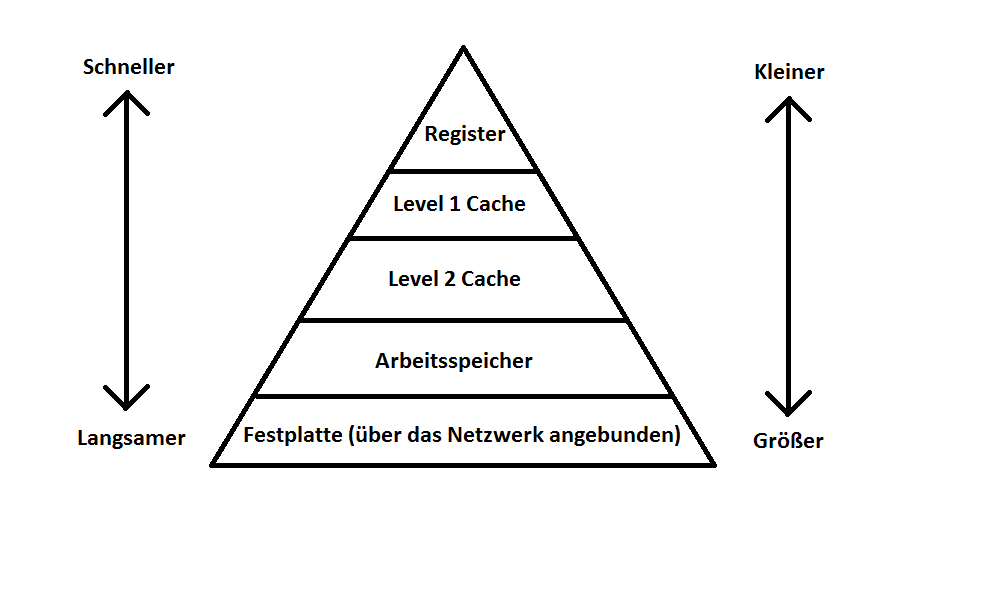
\includegraphics[height=.35\textwidth]{Bilder/hierachie.png}
	\end{center}
	\caption{Die Speicherhierachie des E/A-Systems}
	\label{fig:mem_hierachie}
\end{figure}

Verschiedene Caching-Strategien erlauben eine effizientere Nutzung der Zwischenspeicher.
\begin{itemize}
\item Ein Beispiel für lesende E/A-Aufrufe ist das Einschalten der Read-Ahead-Einstellung, dadurch werden weitere Sektoren in den Cache geladen, die sich in der unmittelbaren physischen Umgebung der angefragten Datenblöcke auf dem  Speichermedium befinden. Falls ein Programm fortlaufend über einen großen Datenbereich arbeitet, weil dort beispielsweise direkt hintereinander Bilddateien eines Fotoalbums befinden, das gerade im Präsentationsmodus gezeigt wird, so ist der Zugriff auf ein weiteres Bild für das E/A-System nicht mehr 'überraschend'. Statt erst in dem Moment des E/A-Aufrufs des nächsten Bildes die erforderlichen Datenblöcke von der Festplatte zu lesen, befinden sich diese nun bereits in einem der vorgeschalteten Zwischenspeicher. Diese Caching-Strategie macht nur Sinn, wenn ein solches sequentielles Zugriffsverhalten eines Programms stattfindet. 
Wenn aufeinanderfolgende Zugriffe in unterschiedlichen Bereichen der Festplatte Datenblöcke anfordern, wird bei dieser Strategie zusätzlicher Aufwand für das Lesen der umgebenden Daten betrieben ohne davon einen Nutzen zu haben (vgl. \cite{corbet2015}). 
\item Eine Caching-Strategie, die eine schnellere Verarbeitung schreibender E/A-Aktionen erlaubt, ist das Wechseln von Write-Through zu Write-Back. Beim Write-Through werden Schreibbefehle, die zunächst nur direkt im Cache umgesetzt werden, direkt in das Speichersystem übernommen. Datenblöcke im Speichersystem und Arbeitsspeicher sind so immer im gleichen und daher widerspruchsfreien Zustand, sodass auch nach plötzlicher Löschung des Caches keine Informationen verloren gehen.
Diese Sicherheit ist beim Write-Back nicht gegeben, da der geänderte Zustand von Daten zunächst nur im Cache bekannt bleibt, damit der Prozessor nicht eine lange Zeit auf die Vollendung des Schreibvorgangs auf der Festplatte warten muss. Das Ausschreiben der Änderungen im Arbeitsspeicher geschieht erst in einem günstigen Moment, wenn beispielsweise ansonsten gerade wenige E/A-Zugriffe geschehen.
\end{itemize}
Entscheidend für die beste Wahl der Cache-Strategien sind jeweils die vorherrschenden Bedingungen im System, sowie dessen Benutzungsweise und die gestellten Anforderungen.

\section{Hochleistungsrechnen}
\label{back_hpc}
Man spricht von Hochleistungsrechnen, wenn der Rechen- oder Speicheraufwand eines Programms außerhalb dessen liegt, was ein einzelner Desktop-Computer in vertretbarer Zeit bearbeiten kann.
Die im Hochleistungsrechnen verwendeten Computer werden als Supercomputer bezeichnet, hierbei handelt es sich heutzutage üblicherweise um Rechnerverbünde (engl. Cluster) in denen eine große Anzahl Prozessoren und Speichermedien zusammengeschaltet werden.
Die übliche Struktur sieht dabei so aus, dass eine Vielzahl Rechnerknoten durch ein gemeinsames Netzwerk zusammengeschaltet werden. Bei einem Rechnerknoten handelt es sich um ein Mehrprozessorsystem mit gemeinsamen Speicher. Jeder Prozessor im Knoten hat einen eigenen Cache mit dem er arbeiten kann, zudem gibt es einen Speicher, auf den alle Prozessoren gemeinsam zugreifen. 
Der Verbund aus Rechnerknoten, der den Hochleistungsrechner bildet, verfügt wiederum über einen gemeinsamen Speicher. Dabei handelt es sich um das Speichersystem des Hochleistungsrechners, das über das Netzwerk mit den einzelnen Rechnerknoten kommuniziert.
\begin{figure}[h]
	\begin{center}
		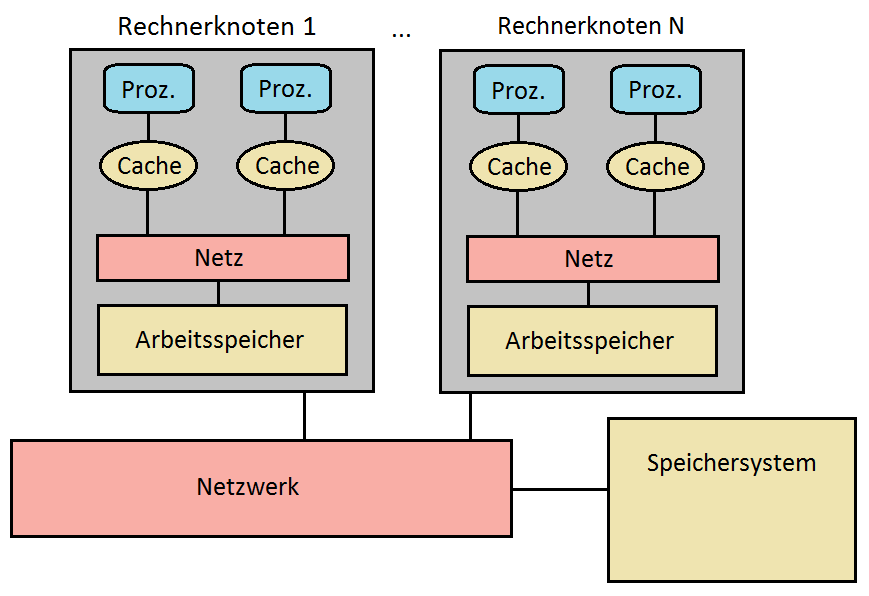
\includegraphics[width=.43\textwidth]{Bilder/rechnerknoten.png}
	\end{center}
	\caption{Struktur des Hochleistungsrechners}
	\label{fig:rechnerknoten}
\end{figure}

Notwendig wird Hochleistungsrechnen in der Forschung für die Simulation von numerischen Modellen aus verschiedensten Bereichen, beispielsweise für Mehrkörpersimulationen in der Astronomie, für Strömungssimulationen oder zur Berechnung von Klimaprognosen.
\medskip

Wichtige Themen im Hochleistungsrechnen sind die effiziente Ausnutzung der zur Verfügung stehenden Leistung, das Erkennen und Beheben von Fehlern des parallelisierten Programmcodes, die Bereitstellung der Rechen- und Speicherkapazitäten, sowie die Energieeffizienz von Hard- und Software.
Um einen Supercomputer gut ausnutzen zu können ist bei vielen Anwendungen eine leistungsfähige Ein-/Ausgabe von großer Wichtigkeit. Bedingt ist dies dadurch, dass die Menge der anfallenden Daten wesentlich stärker ansteigt, als die Geschwindigkeit der Verbindungen zwischen den verschiedenen Speichermedien und -orten.

Die in Abschnitt \ref{back_E/A} beschriebene Ein-/Ausgabe erweitert sich im Rechnerverbund zur parallelen E/A, dies bedeutet einerseits, dass eine Datei von mehreren Prozessen zeitgleich gelesen und bearbeitet werden kann, und andererseits, dass eine Datei über mehrere Festplatten und Netzwerk-Server verteilt sein kann. Diese Parallelität hat einen wesentlichen Einfluss auf die E/A-Leistungsvorhersage, denn statt nur den Aufwand der Arbeitsschritte auf einer einzelnen Festplatte abzuschätzen, müssen hier die verstrickten Zusammenhänge zwischen Netzwerken von Festplatten und Rechnern, den jeweiligen Auslastungen der Komponenten, sowie Priorisierungen bestimmter Aufgaben und Instanzen durch die Speicherverwaltung berücksichtigt werden.

Die Erfassung aller dieser Informationen wäre sehr aufwendig, sodass dies zur Zeit nicht möglich ist. Eine Vorhersage von E/A-Leistung eines parallelen Dateisystems ist daher sehr schwierig.

\section{Maschinelles Lernen}
\label{back_ML}
Maschinelles Lernen gehört zu den Themengebieten künstliche Intelligenz und automatisierte Wissensgenerierung. Verfahren dieser Disziplin versuchen durch intelligentes Lernen von Mustern Vorhersagen und Entscheidungen zu treffen.
Als intelligent wird ein maschinelles Verfahren bezeichnet, dass vorgegebene Informationen nicht auswendig lernt und wiedergibt, sondern von diesen Informationen abstrahiert.
Durch eine globale Sichtweise auf die Daten können Gesetzmäßigkeiten zwischen den Trainingsdaten erkennt werden.
Die Trainingsdaten sind die Informationen, die dem Algorithmus bekannt sind.
Ein Testdatensatz dagegen ist eine Menge von ungesehenen Daten mit denen die Ergebnisse des maschinellen Lernens verglichen werden können.
Ein Attribut ist eine messbare Größe der Objekte, die untersucht werden. Dies könnte beispielsweise bei einem Datensatz über Blumen die Farbe der Blütenblätter sein.
Ein Datenpunkt beschreibt ein spezifisches Objekt (z.B. ein bestimmtes Exemplar der Blume), dazu enthält er einen an der Instanz gemessenen Wert zu jedem Attribut.

Typische Aufgaben des maschinellen Lernens sind die Klassifizierung und Regressionsanalyse von Daten.
\begin{itemize}
\item Es muss zwischen Klassifikation und Klassifizierung unterschieden werden.
\begin{itemize}
\item Als Klassifikation bezeichnet man die Zuordnung eines Objekts mit spezifischen Attributen zu einer bestimmten Gruppe von Objekten mit ähnlichen Attributen.
\item Der zur Klassifikation genutzte Klassifikator ist das Ergebnis einer Klassifizierung.
Zur Klassifizierung können Verfahren des maschinellen Lernens genutzt werden. Bei der Klassifizierung muss von den eigentlichen Objekt-Attributen abstrahiert werden, sodass Muster zwischen den Objekten erkannt werden können. Dann können Klassengrenzen definiert werden, die jeder Klasse einen Bereich des Attribut-Raumes zuordnet. Ein Klassifikator muss die Werte der Attribute eines neuen Objekts, das noch keiner Klasse zugewiesen wurde, anschließend nur mit den Klassengrenzen vergleichen und findet so die passende Zuordnung.
\end{itemize}
\item Regressionsanalyse (oft auch nur Regression) ist ein Verfahren zur Bestimmung der Zusammenhänge von einer spezifischen Zielvariablen zu den übrigen Objekt-Attributen. Wenn in einem Datensatz die Einträge zur Zielvariablen fehlen, können die berechneten Relationen zur Prognose der unbekannten Werte mit Hilfe der bekannten Attribute genutzt werden. Die Zielvariable wird so über die Abhängigkeit zu anderen Variablen durch ein Verfahren des maschinellen Lernens modelliert. Das erhaltene Modell aus dem Verfahren wird auch als Prädiktor bezeichnet. 	
\end{itemize}

Ein Verfahren bzw. Algorithmus des maschinellen Lernens erstellt also ein Modell, welches einerseits Aussagen über die zur Verfügung stehenden Daten trifft und darüber hinaus, abgeleitet aus den inneren Abhängigkeiten der Daten, Aussagen über unbekannte Variablen treffen kann.
Bei der Klassifikation wird eine qualitative Aussage über neue Datenpunkte anhand der Einordnung in Gruppen getroffen.
Beim Regressionsmodell wird dagegen eine quantitative Aussage über die Zusammenhänge zwischen den Attributen der Daten getroffen. Das Modell approximiert einen Wert für ein bestimmtes Attribut neuer Datenpunkte, wenn außer der Zielvariablen alle Attribut-Werte gesetzt sind.  
Klassifizierung und Regression können weitergehend über ihr Lernverhalten unterschieden werden.
Während bei der Regression überwachtes Lernen stattfindet, wird bei der Klassifizierung unüberwacht gelernt. Der Unterschied der beiden Varianten befindet sich in den Informationen die im Trainingsdatensatz enthalten sind.
\begin{itemize}
\item Beim unüberwachten Lernen wird kein bestimmtes Ergebnis erwartet, stattdessen muss der Algorithmus versuchen den Informationen inhärente Abhängigkeiten und Zusammenhänge zu erkennen.
Wenn die Klassenzuordnungen bereits in den Trainingsdaten bekannt wären, hätte das Klassifizierungs-Verfahren nicht viel zu tun. 
Der Klassifizierung steht daher während des Lernprozesses auch keine Rückmeldung über die Güte der gemachten Klassifikation zur Verfügung.
\item Die Instanzen der Trainingsdaten beim überwachten Lernen enthalten auch die gesuchten Werte der Zielvariablen, deren Werte der Algorithmus nach dem Lernvorgang auf dem Testdatensatz vorhersagen soll.
Für die Regressionsanalyse sind diese Informationen essentiell, da für die Modellierung die Zusammenhänge der Werte der Zielvariablen mit den restlichen Variablen untersucht werden muss.
Die Information über die idealen Ausgabewerte zur Zielvariablen werden während des Lernvorgangs genutzt um die Parameter des Prädiktors so anzupassen, dass er die vorgegebenen Werte möglichst gut approximiert. Wichtig ist dabei, dass der Prädiktor nicht zu sehr auf die Trainingsdaten zugeschnitten wird, sondern die abstrakteren Relationen erkennt, sodass auch auf den ungesehenen Testdaten gut vorhersagen gemacht werden können.
\end{itemize}

Die vom Klassifikator erstellten Gruppierungen werden üblicherweise nicht bewertet, da die Qualität einer Sortierung nur im Kontext des gewünschten Nutzens der Klassen beurteilt werden kann.
Zunächst einmal ist jede eindeutige Klassifizierung legitim.

Der Prädiktor der Regressionsanalyse kann dagegen konkret bewertet werden. Dazu wird der Testdatensatz benötigt. Die zu bestimmenden Werte der Zielvariablen sind in den Testdaten bereits vorgegeben.
Diese Information wird bei der Durchführung des Tests vorenthalten. Durch den Vergleich zwischen tatsächlicher und vorhergesagter Lösung können Rückschlüsse auf die Qualität der Vorhersagen gezogen werden können. Dazu werden Metriken zur Bestimmung der Güte der Modellierung benötigt.
Zur Anwendung einer Regressionsanalyse müssen also zunächst Kriterien bzw. Leistungsmetriken eingeführt werden, anhand derer die Qualität der Vorhersagen und Entscheidungen gemessen werden können. Einerseits zum Vergleich der Vorhersagen auf den Testdatensatz zwischen verschiedenen Ansätzen, andererseits aber auch schon für den Lernprozess des Algorithmus selbst, damit dieser sozusagen aus seinen Fehlern und Erfolgen lernen kann. Eine einfache Metrik wäre beispielsweise die mittlere Modellabweichung der Vorhersagen gegenüber den \textit{Lösungswerten}.
\medskip

Oft ist es notwendig die zur Verfügung stehenden Daten aufzubereiten, bevor ein maschineller Lernalgorithmus effizient und korrekt Informationen aus diesen ableiten kann.
Nach Alpaydin können fehlerhafte Daten ein Problem sein, die durch zufällige Messfehler oder eine systematisch inkorrekte Messung entstehen können (vgl. \cite{Alpaydin:2010:IML:1734076} S. 13-15). Zudem schreibt er, dass Teile der Daten überflüssig sein können, da sie redundant sind oder keine relevanten Informationen enthalten. Problematisch sind auch Datenpunkte mit gleichen Eingabewerten, aber unterschiedlichen Werten zur Zielvariablen (vgl. \cite{Alpaydin:2010:IML:1734076} S. 14).
Mit all diesen Problemen muss, unter Beachtung der Eigenschaften des vorliegenden Datensatzes, bei der Aufbereitung der Daten sinnvoll umgegangen werden. So können beispielsweise Ausreißer bei den Daten aussortiert werden, da diese eventuell durch eine Fehlmessung entstanden sind. Widersprüchliche Datenpunkte können zusammengefasst werden, indem sie zusammen einen neuen Datenpunkt mit eindeutigen Ausgabewerten bilden (dies könnten die Mittelwerte sein).

\subsubsection{Clusteranalyse}
Eine typische Anwendung der Klassifizierung ist die Clusteranalyse.
Kantardzic beschreibt Clusteranalyse folgendermaßen: \glqq Cluster analysis is the formal study of methods and algorithms for natural grouping, or clustering, of objects according to measured or perceived intrinsic characteristics or similarities.\grqq{} \cite{kantardzic2011data} (S. 250). Ein einfaches und anschauliches Beispiel sind Punkte im zweidimensionalen Raum, die hinsichtlich ihrer Position gruppiert werden (siehe Abbildung \ref{fig:clustering_beispiel}).

\begin{figure} [h]
	\subfloat{
		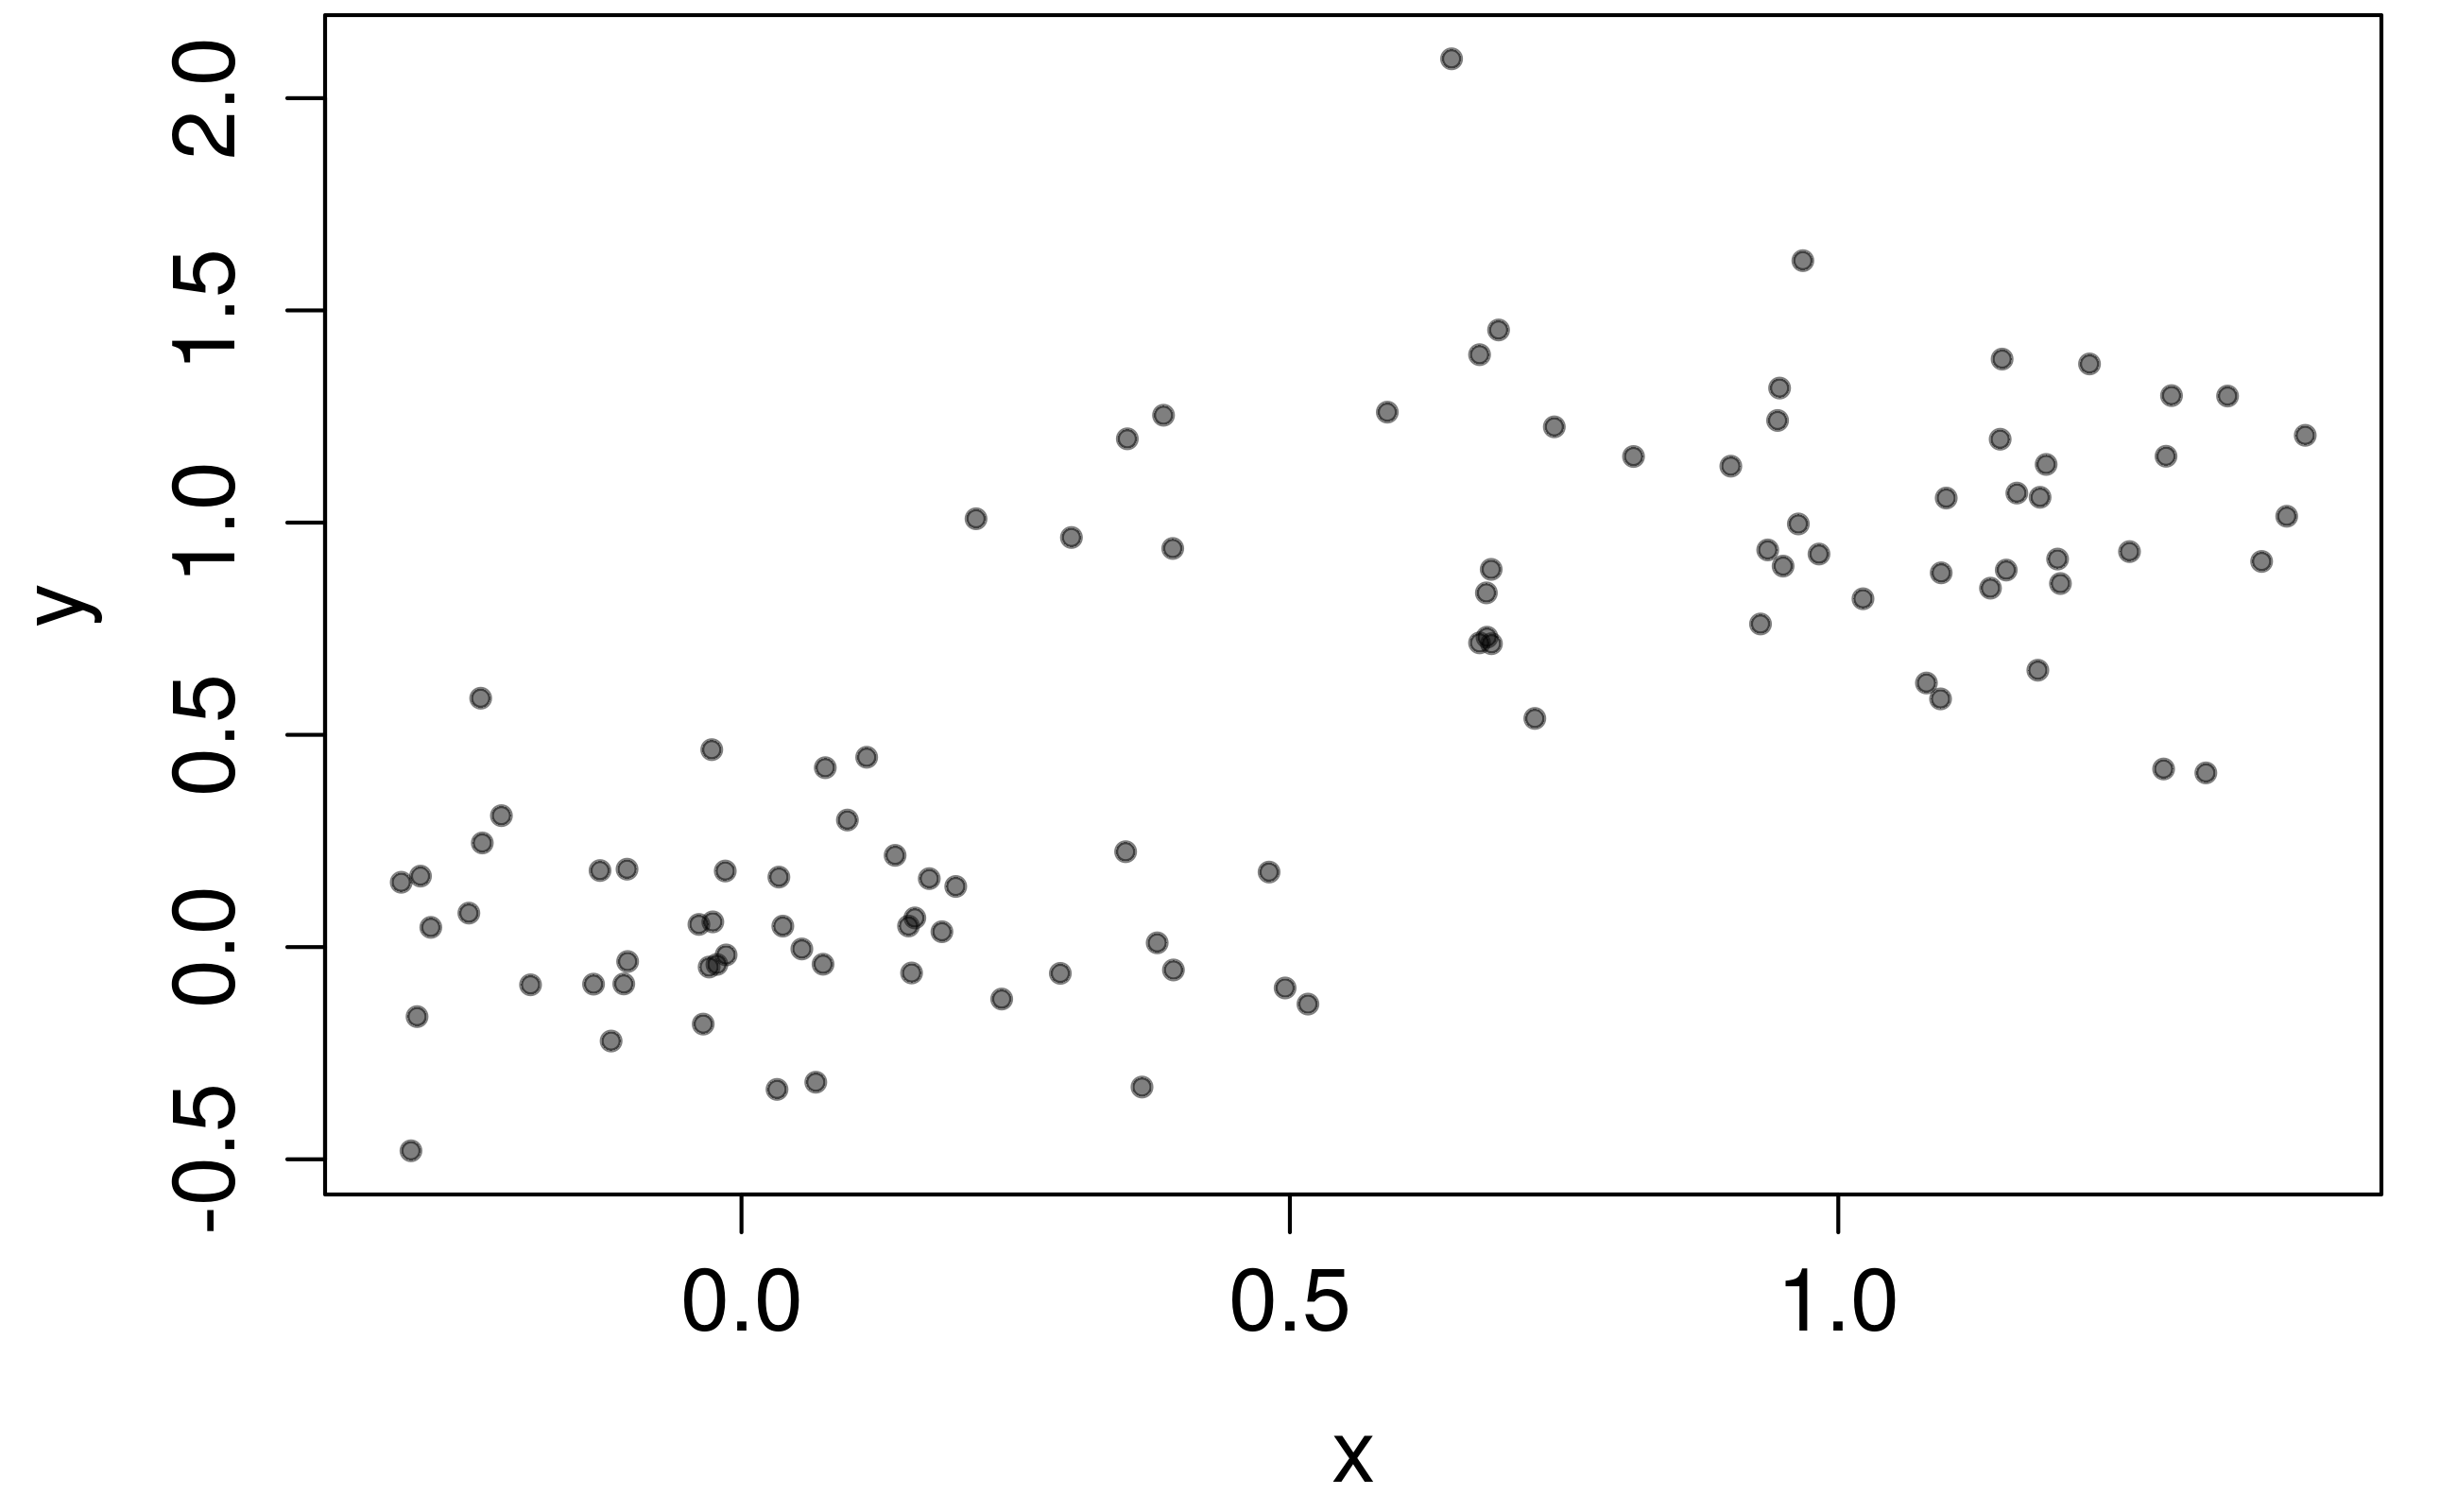
\includegraphics[width=.5\textwidth]{Bilder/test_clustering_points.png}
	}
	\hfill
	\subfloat{
		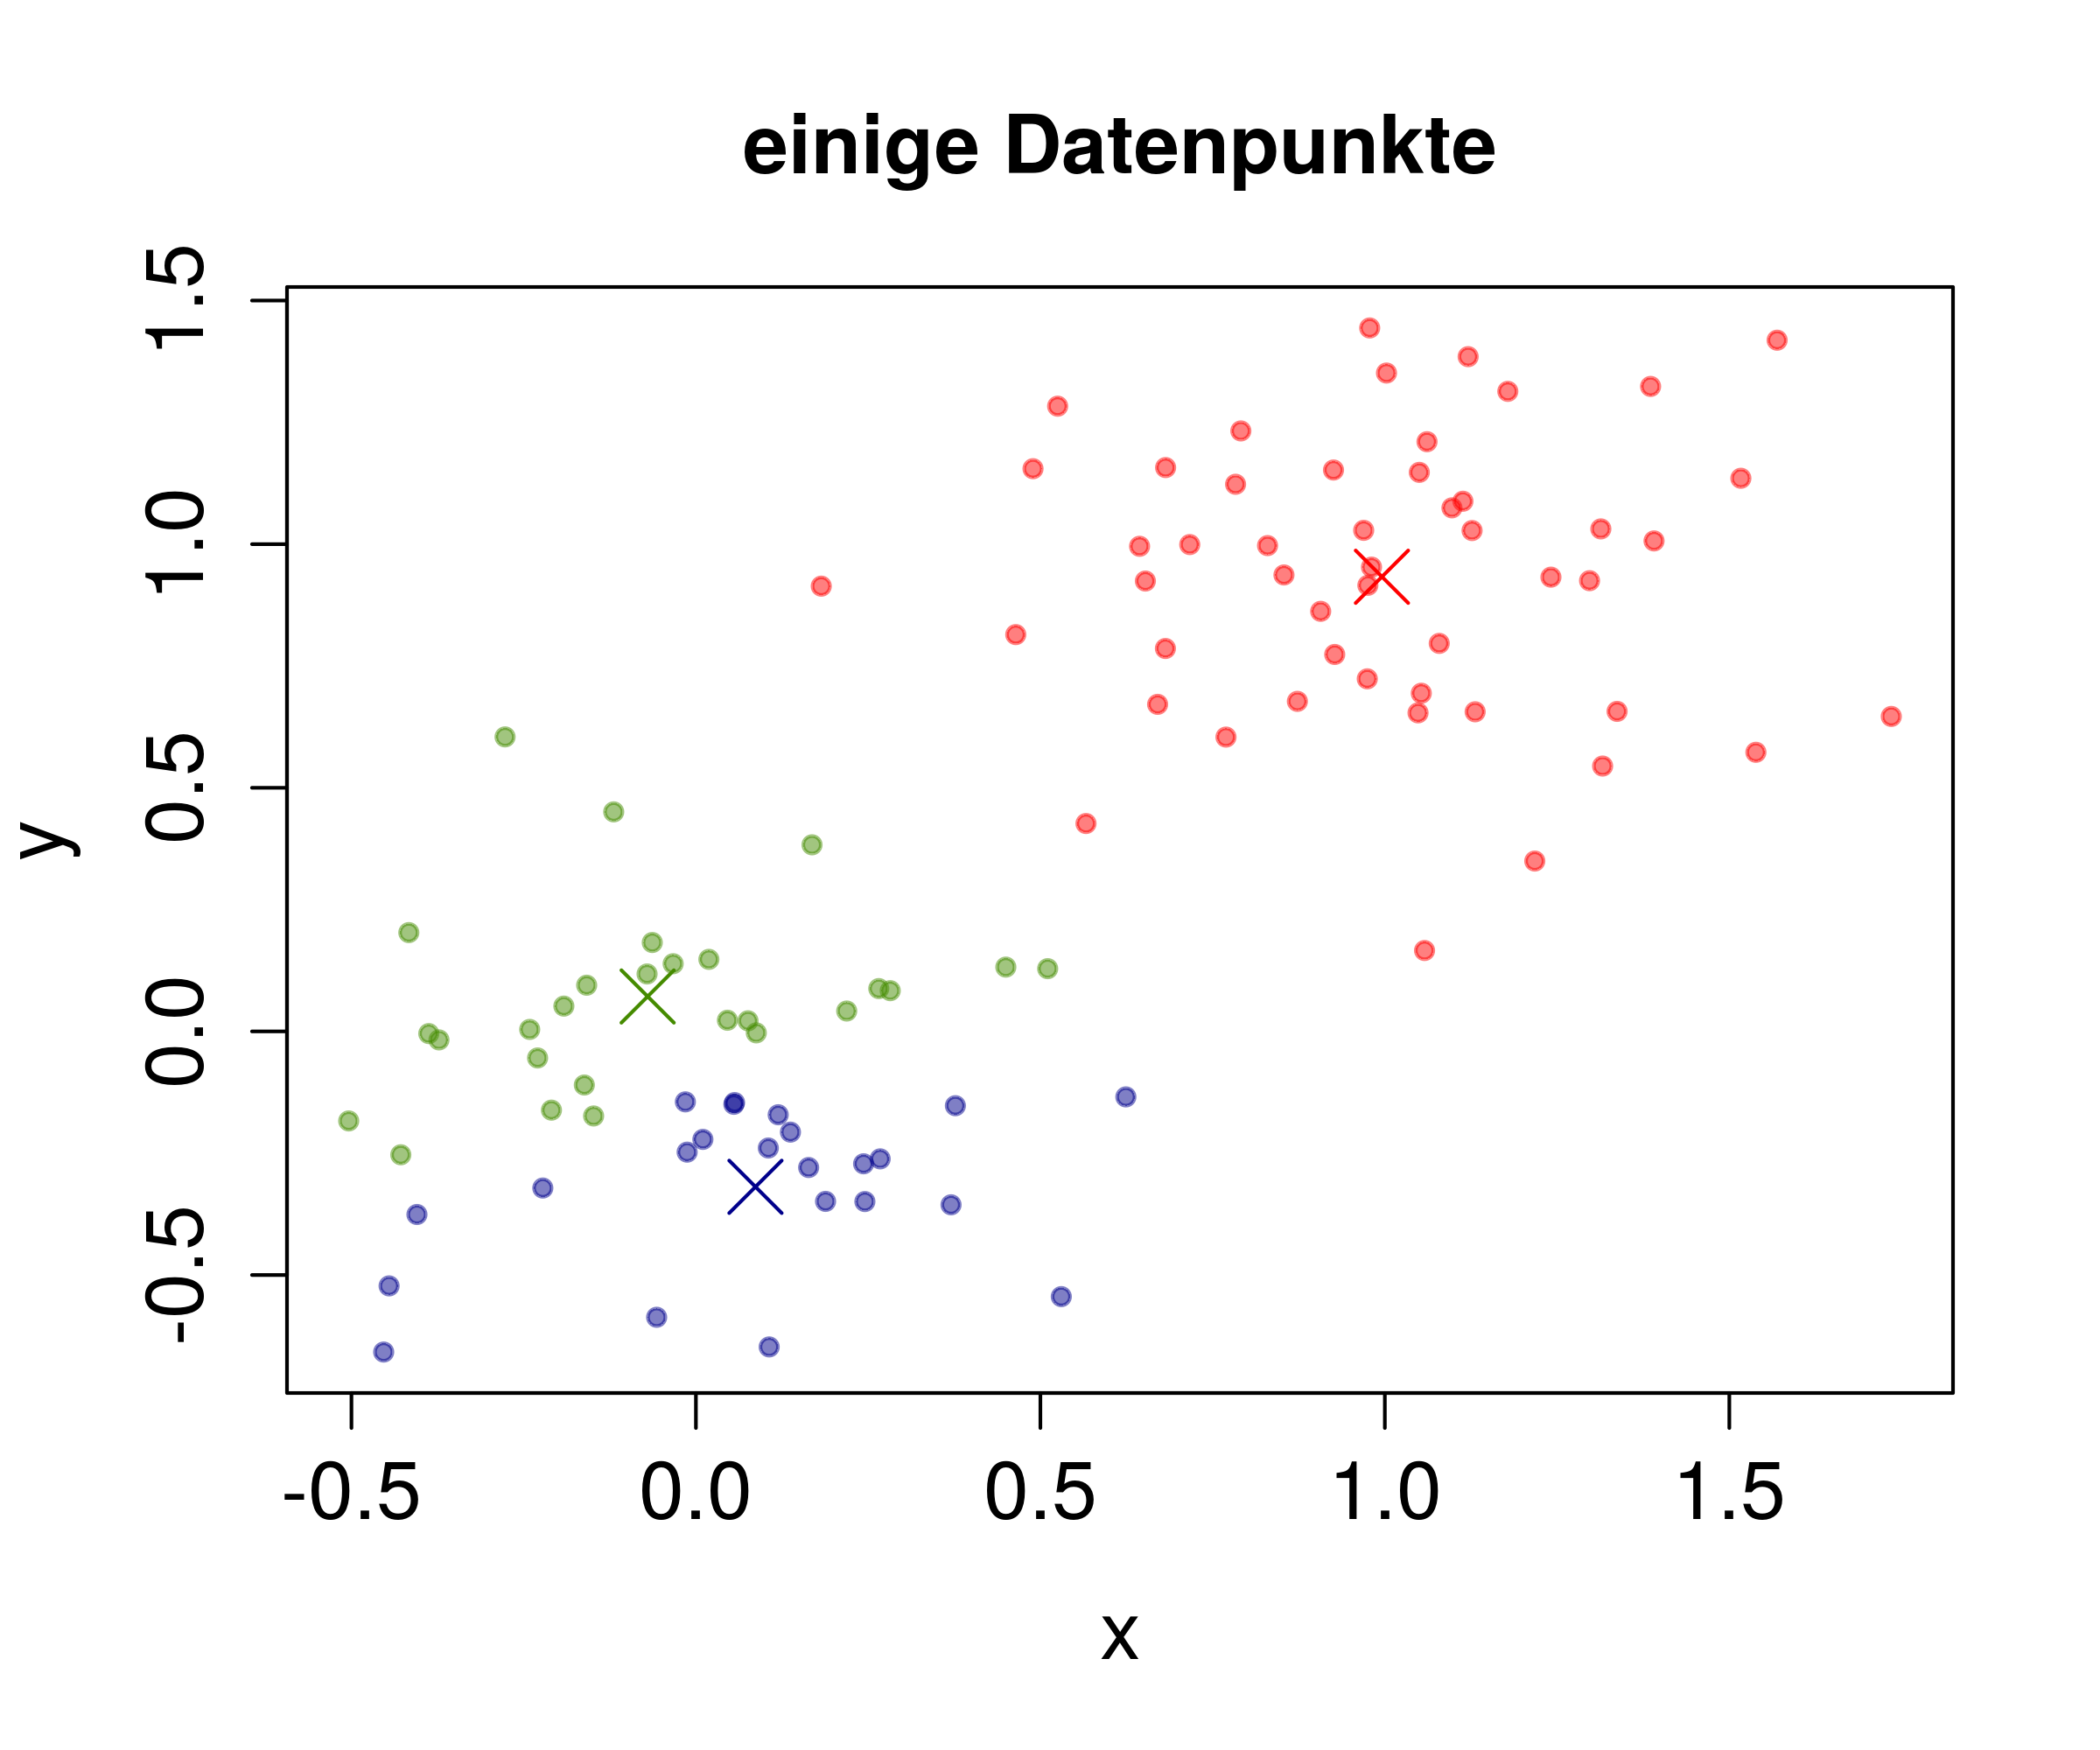
\includegraphics[width=.5\textwidth]{Bilder/test_clustering.png}
	}	
	\caption{Datenpunkte mit je einem Wert für x und y-Dimension. Rechts farbliche Markierung für die Zugehörigkeit zu den drei vom k-Means-Algorithmus bestimmten Clustern. Ein Kreuz markiert den Mittelpunkt jedes Clusters (Mittelwert aller zugehörigen Punkte)}
	\label{fig:clustering_beispiel}
\end{figure} 

Ein einfacher Clustering-Algorithmus ist der k-Means-Algorithmus. Bei diesem muss zunächst die Anzahl Cluster $k$ festgelegt werden. Die $k$ Mittelwerte der Cluster werden mit zufälligen Werten initialisiert. Dann wird jeder Datenpunkt dem Cluster zugeordnet, dessen Mittelwert seinem am dichtesten ist. Danach werden die Mittelwerte der Cluster anhand der Ihnen zugeordneten Punkte berechnet und gesetzt. Das Neuzuordnen der Punkte und Berechnen der Mittelwerte wird nun solange wiederholt, bis sich keine Änderung der Zuordnung mehr ergibt. Als Endergebnis eines Cluster-Algorithmus erhält man eine Gruppierung der Datenpunkte in Mengen mit möglichst niedriger Varianz innerhalb eines Clusters und möglichst großer Varianz zwischen den Clustern.

\section{Künstliche Neuronale Netze}
\label{back_nn}
Bei künstlichen neuronalen Netzen, im Folgenden nur neuronale Netze genannt, handelt es sich um eine Methode aus dem Bereich des maschinellen Lernens zum Approximieren einer unbekannten Funktion, die der Relation zwischen zwei Datenmengen zugrunde liegt. Die Methode ist inspiriert von biologischen neuronalen Netzen, wie sie im Gehirn vorkommen. 
Sie verwenden einen statistischen Ansatz, ihre Lösung für das Problem wird zunächst zufällig im Lösungsraum angelegt und dann mit Hilfe eines Gradientenverfahrens optimiert.
Rojas vergleicht neuronale Netze mit einer Black Box, also einem System mit beobachtbarer Ein- und Ausgabe, aber unbekannter innerer Verarbeitung der Informationen \cite{Rojas:1996:NNS:235222}. 
Zur Verwendung eines neuronalen Netzes gibt man dem Netz eine Menge von Eingabevektoren $E \in \mathbb{R}^n$ mit jeweils zugehörigem Ausgabevektor $A \in \mathbb{R}^m$ vor und dieses versucht eine passende Funktion $F: \mathbb{R}^n \rightarrow \mathbb{R}^m$ zu finden. Dementsprechend handelt es sich hierbei um überwachtes Lernen, da eine gewünschte ideale Ausgabe vorgegeben wird.

\begin{figure}[h]
	\begin{center}
		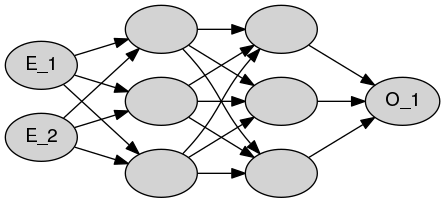
\includegraphics[height=.20\textwidth]{Dot/netz.png}
	\end{center}
	\caption{feedforward-Netz mit $n=2$, $m=1$ und 2 verborgenen Schichten}
	\label{fig:Schichten}
\end{figure}

Die häufigste verwendete Art neuronaler Netze sind feedforward-Netze. Sie bestehen aus einer Eingabeschicht, einer beliebigen Anzahl verborgener Schichten und einer Ausgabeschicht (siehe Abbildung \ref{fig:Schichten}), wobei die Verbindungen aus jeder Schicht jeweils nur in die Nächsthöhere gehen. 
Die Eingabeschicht besteht, meiner vorherigen Definition entsprechend, aus $n$ Stellen, an denen die Werte eines Eingabevektors stehen. Jeder Eingabewert wird dann an jedes Neuron in der ersten verborgenen Schicht weitergegeben und dort verrechnet, die Ergebnisse der Neuronen der verborgenen Schicht werden dann an die nächste Schicht gegeben und so weiter.
Die Ergebnisse der Ausgabeschicht bilden den Ausgabevektor mit Länge $m$.
Rekurrente Netze haben die gleiche Struktur, doch es können auch Verbindungen zu zurückliegenden Schichten vorkommen, dadurch ist die Berechnung zu einem Eingabevektor nicht mehr deterministisch bestimmt. Es müssen Berechnungs- und Determinierungsregeln festgelegt werden. 

\begin{figure}[h]
	\begin{center}
		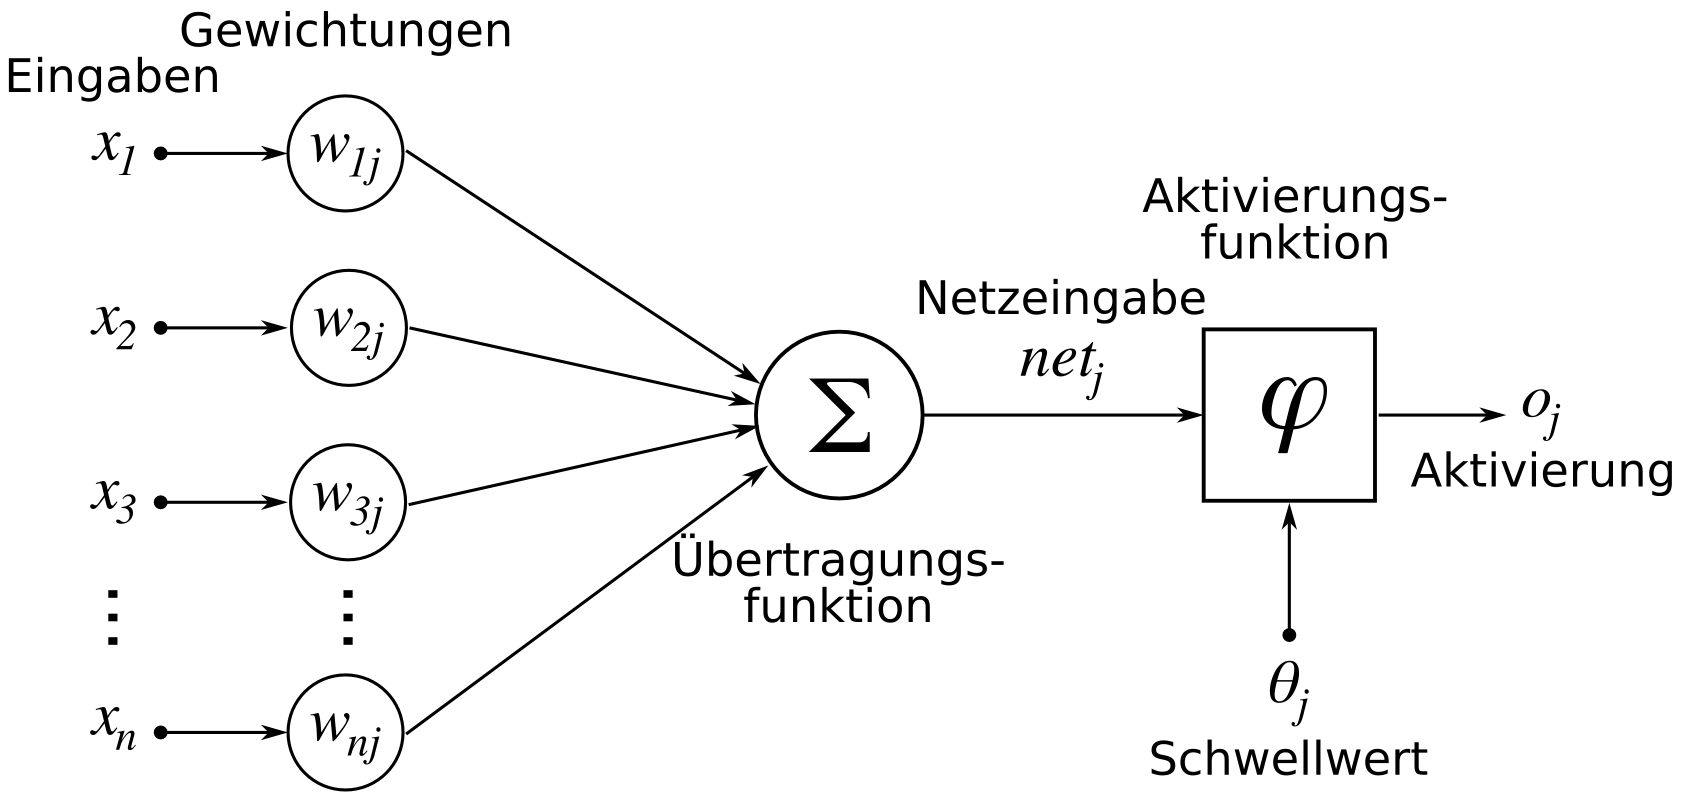
\includegraphics[totalheight=0.2\textheight]{Bilder/ArtificialNeuronModel_deutsch.png}
	\end{center}
	\caption{Schema eines künstlichen Neurons. Quelle: Chrislb, \url{https://de.wikipedia.org/wiki/Datei:ArtificialNeuronModel_deutsch.png}} %
	\label{fig:Neuron}
\end{figure}

Jedes Neuron rechnet die eingehenden Eingabewerte mit einer zur Übertragungskante zugehörigen Gewichtung mit einer Übertragungsfunktion zusammen; die Anzahl der Eingaben ist hierbei unbegrenzt (vgl. \glqq unlimited fan-in property\grqq{} \cite{Rojas:1996:NNS:235222}). Die Übertragungsfunktion kann hierbei schlicht die Summe aller gewichteten Eingaben sein. Der errechnete Wert wird als Netzeingabe an die Aktivierungsfunktion gegeben. 
Die Aktivierungsfunktion berechnet eventuell mit oder ohne einem Schwellwert die Aktivierung des Neurons, welche dann an alle verbundenen Neuronen der nächsten Schicht weitergegeben wird.
Die Aktivierungsfunktion kann beispielsweise eine simple Stufenfunktion sein, die allen Netzeingaben kleiner des Schwellwerts eine Null und allen Eingaben größer gleich des Schwellwerts eine Eins zuweist.

Ein Neuron mit der gewichteten Summe aller Eingaben als Übertragungsfunktion und einer Stufenfunktion mit Schwellwert als Aktivierungsfunktion wird von Rojas \textit{Perzeptron} bezeichnet (vgl. \cite{Rojas:1996:NNS:235222} S. 60).
\medskip

Ein feedforward-Netzwerk aus Perzeptrons, in dem jedes Neuron mit allen Neuronen der folgenden Schicht verbunden ist, wird als \textit{multilayer perceptron} (kurz MLP) bezeichnet.

\subsubsection{Trainieren von neuronalen Netzen}
Ein neuronales Netz lernt die Abbildung zwischen den vorgegebenen Paaren von Eingabe- und Ausgabedaten durch Anpassung der Gewichte an den Kanten, nachdem es mit zufälligen Kantengewichten initialisiert wurde.
Diese Anpassung geschieht beim MLP durch Fehlerrückführung (engl. backpropagation). Dabei wird der mittlere quadratische Fehler der berechneten Ausgabe gegenüber der vorgegebenen idealen Ausgabe ermittelt und daraufhin unter Rücksichtnahme auf eine Lernrate mit Hilfe des Gradientenverfahren minimiert.

\subsubsection{Berechenbarkeitstheorie neuronaler Netze}
Vor der Anwendung von künstlichen neuronalen Netzen für ein Problem stellt sich die Frage, ob diese für das Problem geeignet sind. Dazu gibt es einige interessante mathematische Beweise.
Ein einzelnes Perzeptron kann alle linear separierbaren logischen Funktionen exakt approximieren (vgl. \cite{Rojas:1996:NNS:235222} S. 62-63), wobei lineare Separierbarkeit nach Rojas definiert ist als:

Zwei Punktmengen A und B in einem n-dimensionalen Raum sind linear separierbar, wenn $n + 1$ reelle Zahlen $w_1,...,w_{n+1}$ existieren, sodass für jeden Punkt $(x_1,x_2,...,x_n) \in A$ die Ungleichung $\sum_{i=1}^{n} w_ix_i \ge w_{n+1}$ gilt und für jeden Punkt $(x_1,x_2,...,x_n) \in B$ $\sum_{i=1}^{n} w_ix_i < w_{n+1}$

\begin{figure}
	\subfloat[Zwei voneinander nicht linear separierbare Relationen in $ \mathbb{R}^2$.]{
		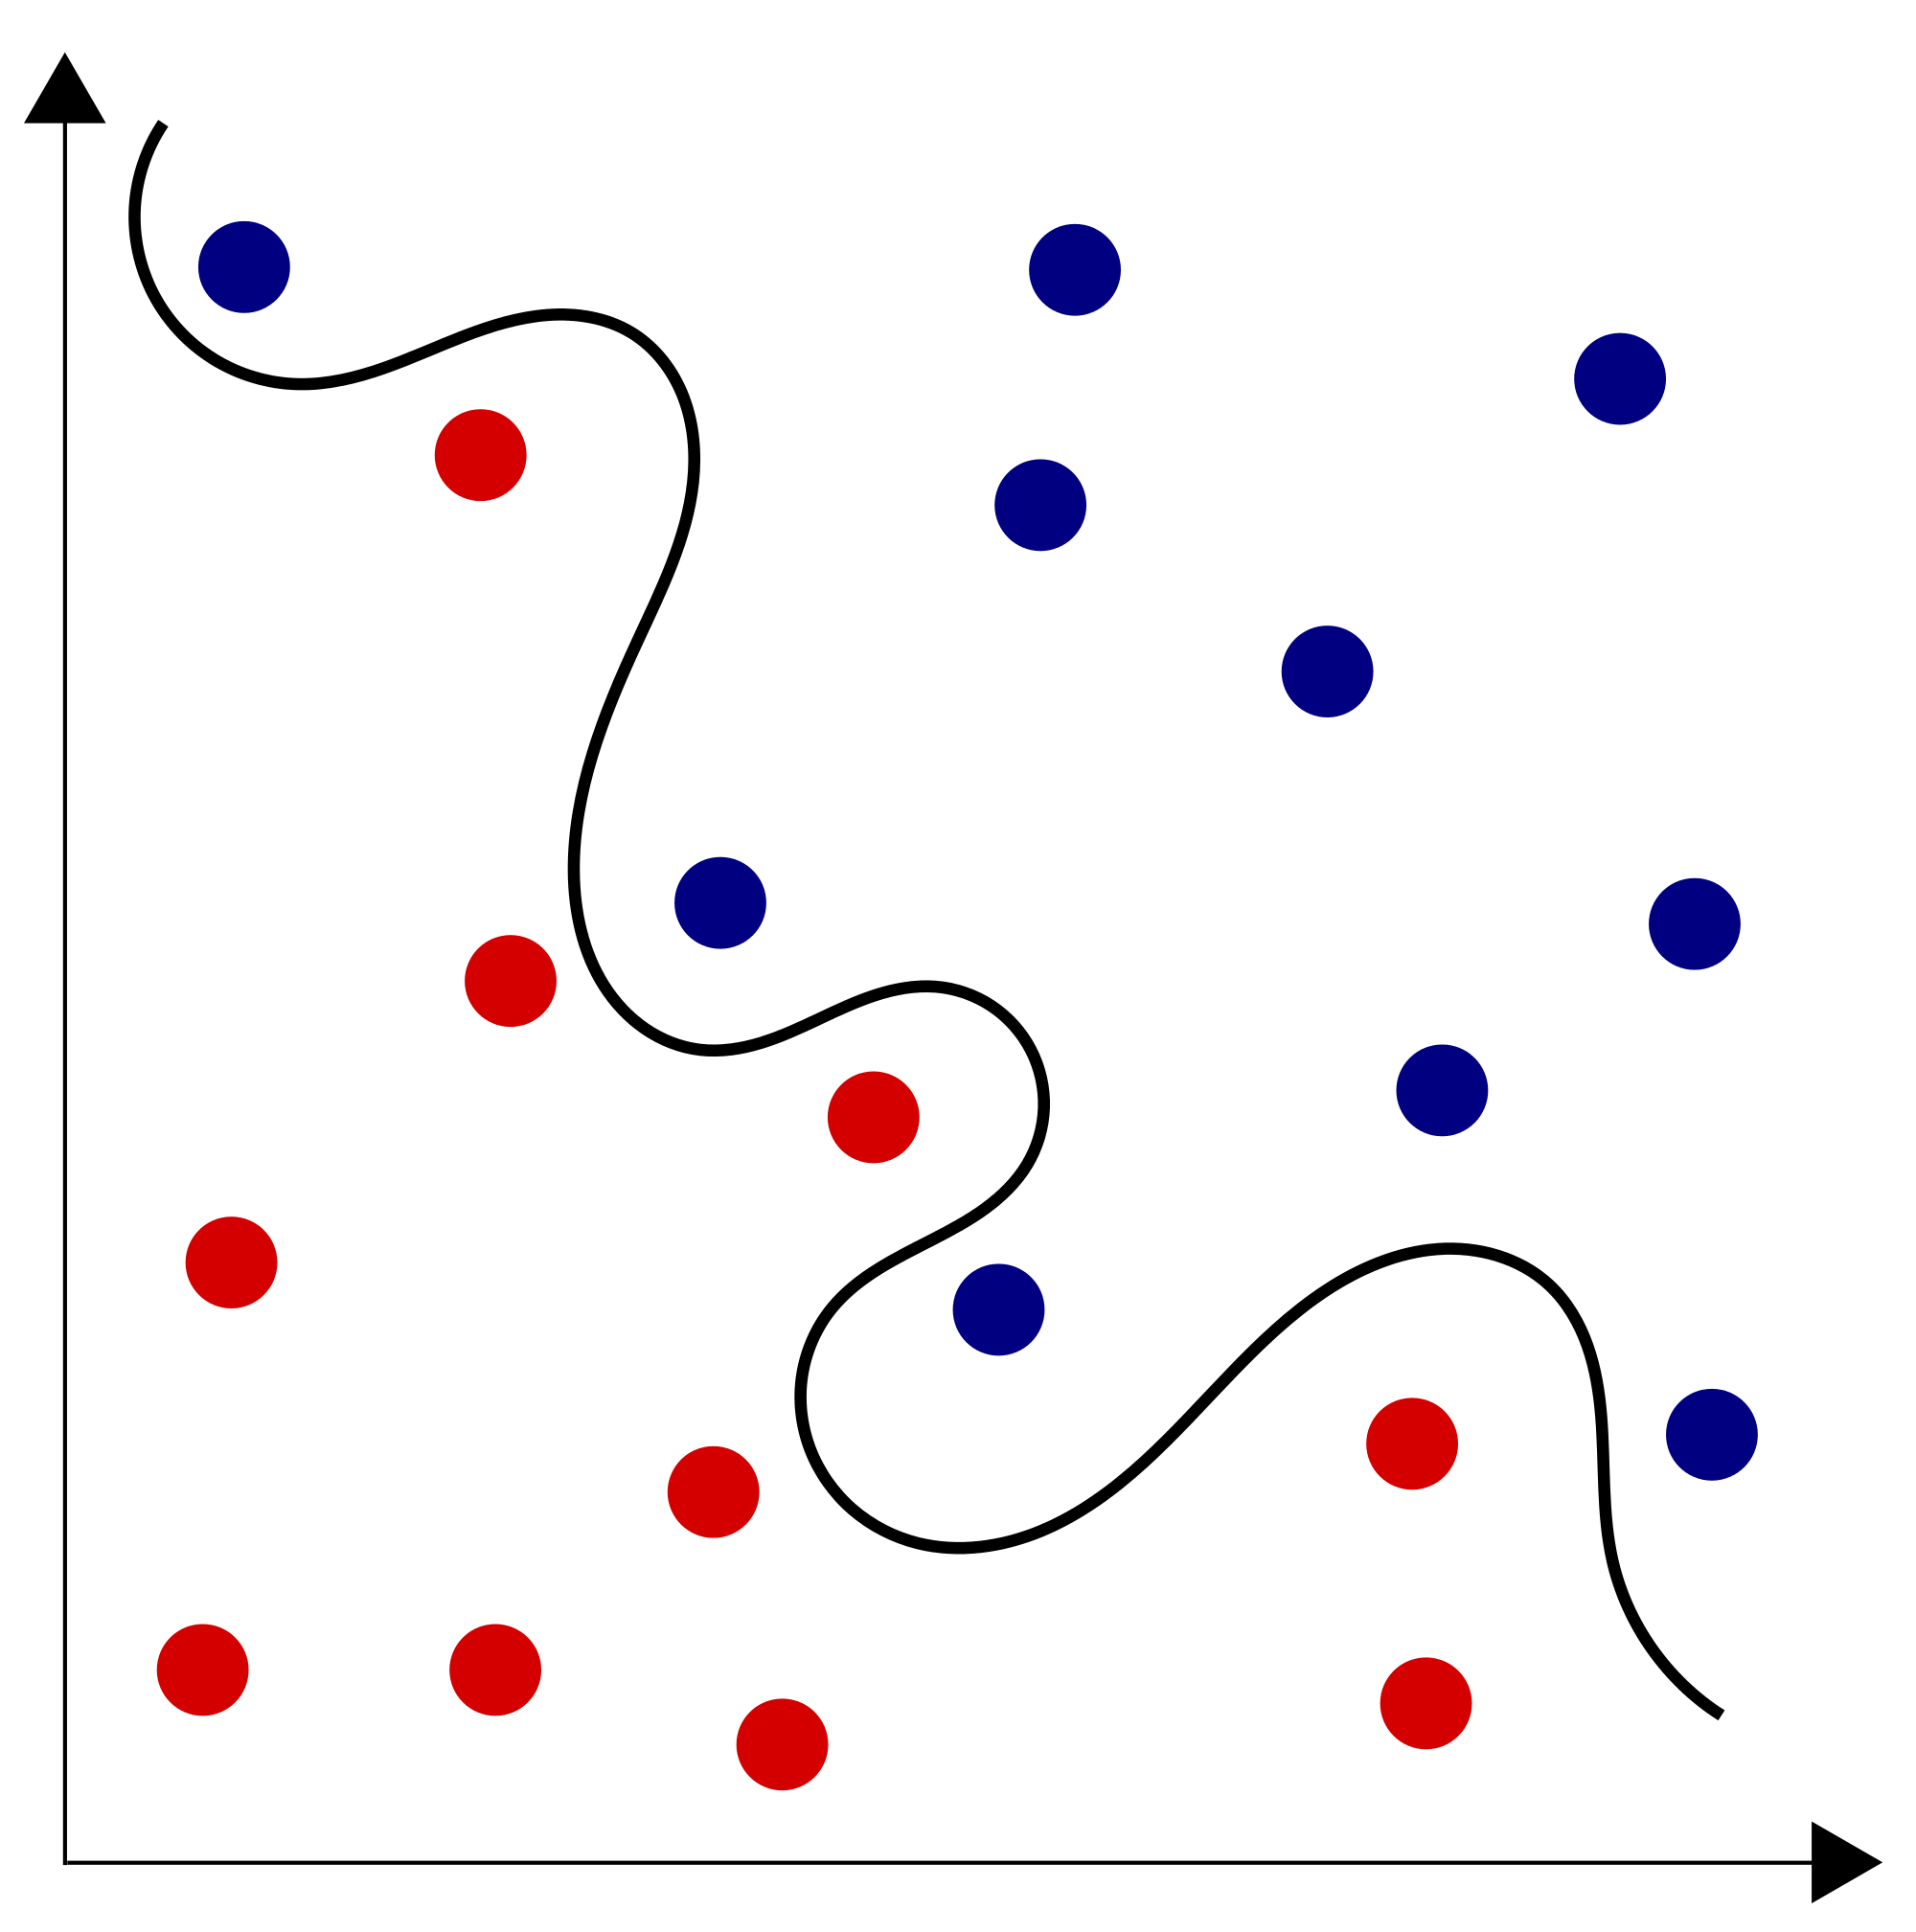
\includegraphics[width=.3\textwidth]{Bilder/2000px-Separability_NO.png}
	}
	\hfill
	\subfloat[Zwei voneinander linear separierbare Relationen in $\mathbb{R}^2$.]{
		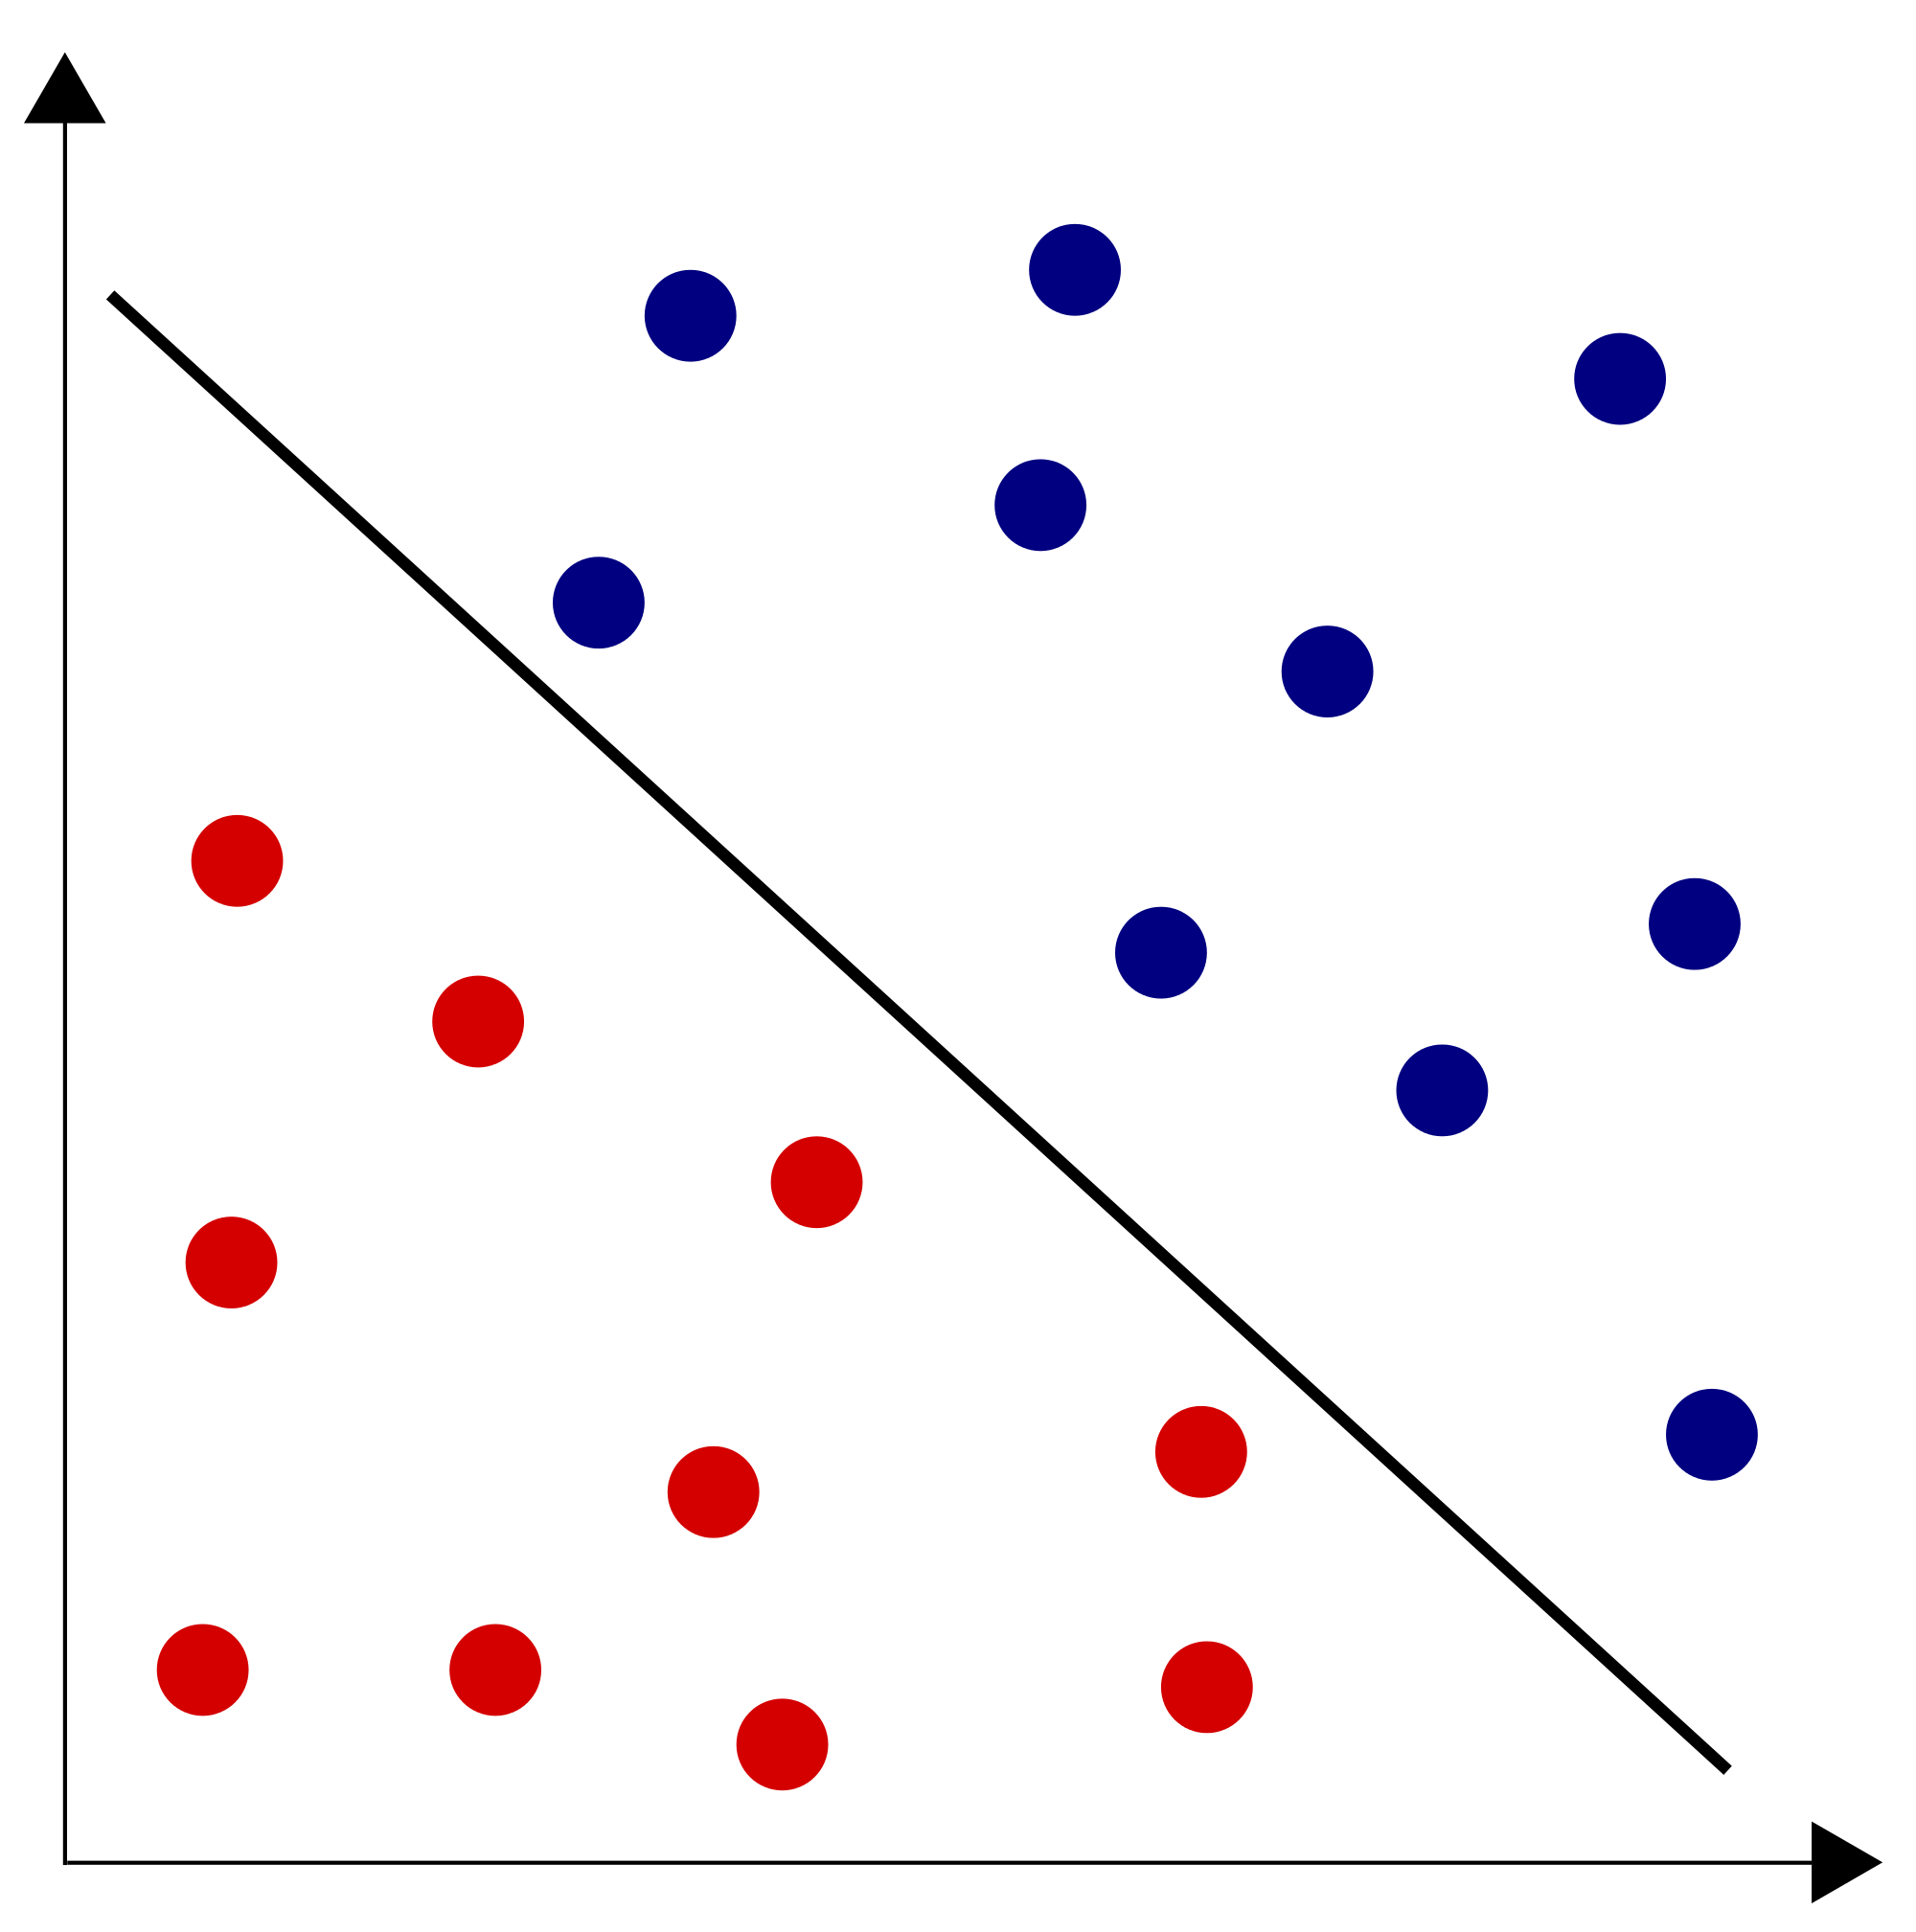
\includegraphics[width=.3\textwidth]{Bilder/2000px-Separability_YES.png}
	}		
	\caption{Lineare Separierbarkeit, Quelle: Mekeor, \url{https://de.wikipedia.org/wiki/Datei:Separability_YES.svg} und \url{https://de.wikipedia.org/wiki/Datei:Separability_NO.svg}}
	%
	\label{fig:separierbarkeit}
\end{figure} 

Diese Beschränkung gilt allerdings nicht für ein Netzwerk von Neuronen. Bereits ein zweilagiges Netzwerk aus noch simpleren McCulloch-Pitts-Zellen kann jede beliebige logische Funktion berechnen (vgl. \cite{Rojas:1996:NNS:235222} S. 37).
Für MLPs hat Cybenko \cite{cybenko:mcss} bewiesen, dass sie beliebige kontinuierliche Funktionen auf einer kompakten Teilmenge des euklidischen Raums $\mathbb{R}^n$ approximieren können. Der entsprechende Satz hierzu ist das \textit{universal approximation theorem}.

\bigskip
\paragraph{Zusammenfassung:}
\textit{ 
	Das Kapitel hat einen kurzen Abriss der für diese Thesis relevanten Themen geliefert. Es wurde festgestellt, dass die Vorhersage von E/A-Laufzeiten im Hochleistungsrechnen eine komplexe Aufgabe ist. Zusätzlich zu dem ohnehin aufwendigen E/A-System eines normalen Rechners müssen die Komplikationen durch die Vernetzung des Hochleistungsrechners in Betracht gezogen werden.\\
	Das Problem der E/A-Leistungsvorhersage kann mit Hilfe maschinellen Lernens gelöst werden. Die Aufgabe entspricht dabei einer Regressionsanalyse. Durch Vorgabe gemessener Zugriffszeiten von E/A-Aufrufen kann überwachtes Lernen betrieben werden. Dabei werden die Abhängigkeiten zwischen Aufrufparametern und Zugriffszeit ausgenutzt um die unbekannten Laufzeiten unbekannter Zugriffe vorherzusagen.
	Solange die E/A-Leistung durch eine kontinuierliche Funktion beschrieben werden kann und alle dafür benötigten Informationen zur Verfügung stehen, kann ein künstliches neuronales Netz das Problem lösen.
}

\chapter{Verwandte Arbeiten}
\textit{%
	In diesem Kapitel werden wissenschaftliche Veröffentlichungen vorgestellt, die dieser Arbeit gegenüber relevante Themen behandeln. Es werden drei Teilgebiete des Problems der Leistungsvorhersage von E/A-Aufrufen im Hochleistungsrechnen behandelt.\\
	Als Erstes gehe ich in Abschnitt \ref{rel_ea-vorhersage} auf einige Arbeiten ein, die allgemeine E/A-Leistungsvorhersage behandeln. Dabei führe ich zunächst zwei Begriffe für Kategorien von Lösungsansätzen ein. Danach gehe ich in Unterkapitel \ref{rel_vorhersage-mit-nn} auf Arbeiten ein, die sich mit der Verwendung von neuronalen Netzen zur Leistungsvorhersage beschäftigen.
	Und in Abschnitt \ref{rel_vorhersage_im-hpc} werden Veröffentlichungen diskutiert, die Leistungsmodellierung speziell im Hochleistungsrechnen behandeln.
}
\bigskip

\section{Leistungsvorhersage von Ein-/Ausgabe}
\label{rel_ea-vorhersage}
Das Problem, die Zugriffszeiten auf Festplatten vorherzusagen, kann im wesentlichen durch zwei verschiedene Ansätze gelöst werden (vgl. \cite{Crume:2013:FML:2538542.2538561} S. 45).
\begin{itemize}
\item  Zum Einen kann man versuchen das Festplattensystem in einem Modell nachzubilden, indem Hardwaredetails, wie die Rotationsgeschwindigkeit der Platte, die Reaktionszeit und Geschwindigkeit des Lesekopfs, sowie das Zusammenspiel der Komponenten bekannt sind oder entsprechende Parameter durch gezielte Untersuchung approximiert werden. Mit diesem möglichst exakten Modell können dann Zugriffe simuliert und die Laufzeit des Modells gemessen werden. Diese Messung kann daraufhin als Vorhersage für das reale System verwendet werden. Eine White-Box ist ein System dessen innere Funktionsweise bekannt ist. Modelle dieses Ansatzes können entsprechend als White-Box-Modelle bezeichnet werden.
\item Beim zweiten Ansatz wird vom eigentlichen Festplattensystem abstrahiert und stattdessen ein mathematisches Modell gesucht, das das Verhalten des Systems möglichst genau beschreibt.
Zur Entwicklung des mathematischen Modells wird eine Regressionsanalyse durchgeführt. Dabei werden gemessene Leistungswerte von Festplattenzugriffen untersucht, um daraus passende Parameter für das Modell abzuleiten. Analog zur vorherigen Namensgebung kann dieser Ansatz als Black-Box-Modellierung bezeichnet werden, da hier ohne Wissen über die inneren Zustände des Systems modelliert wird.
\end{itemize}
Ich unterscheide daher im Folgenden zwischen der White-Box-Modellierung, bei der versucht wird das Festplattensystem nachzubilden (in der englischen Fachliteratur auch als \textit{analytic device modeling} und \textit{simulation modeling} bezeichnet) und der Black-Box-Modellierung, bei dem ein mathematisches Modell entwickelt wird.

\subsubsection{White-Box-Modellierung gegenüber Black-Box-Modellierung}
Die Nachteile von Modellen der White-Box-Modellierung liegen insbesondere darin, dass sie aufwendig zu konfigurieren sind. Beispielsweise schreiben Crume et al.:\glqq In fact, one of us (Oldfield) spent several months configuring DiskSim to model an existing device\grqq{} \cite{Crume:2013:FML:2538542.2538561} (S.45). Naturgemäß altern White-Box-Modelle schnell, da sie jeweils an spezielle Hardware angepasst sind. Der Vorteil dagegen ist, dass sie bei korrekter Konfiguration sehr präzise sind. Ruemmler und Wilkes erzielten mit einem gut kallibrierten White-Box-Modell geringe Residuen bei der Vorhersage von Festplatten-Zugriffszeiten (vgl. \cite{Ruemmler94anintroduction}). Um das Problem des hohen Aufwands der exakten Parametriesierung für jedes Festplattenmodell anzugehen, haben sie untersucht, wie sich die Berücksichtigung verschiedener Festplattenkomponenten bzw. -eigenschaften auf den Modellfehler auswirkt. Sodass beim Einsatz des Modells Aufwand der Parametriesierung und Präzision der Modellierung gegeneinander abgewägt werden können.

Eine weitere Arbeit, in der White-Box-Modellierung genutzt wurde, stammt von Lebrecht et al. \cite{Lebrecht:2009:10.1109/QEST.2009.31}. Darin wird besonders auf ein Verfahren eingegangen, das dafür sogt, dass E/A-Anfragen in einer Reihenfolge abgearbeitet werden, die die notwendigen Bewegungen des Lese-/Schreibkopfes möglichst gering hält.
\medskip

Die Black-Box-Modellierung ist in der Anwendung einfacher und flexibler, da sie automatisch an das System anpasst werden kann. Dafür erwartet man aufgrund der fehlenden analytischen Einsicht ins System ungenauere Prognosen. Für die Anwendung im HPC-Bereich spielt der analytische Ansatz eine untergeordnete Rolle, da hier unterschiedliche Festplattensysteme zusammenarbeiten und stark mit der Netzwerkarchitektur verstrickt sind, sodass eine entsprechende Analyse des Systems aufwendig wird: \glqq Furthermore, the technical trend towards storage consolidation in large data centers hints that building an accurate model or simulator using white box method cannot be a genereal solution in serving a variety of very different workloads\grqq{} \cite{DBLP:conf/npc/ZhangLZJC10} (S.122, Zeile 20-24).

Bei Arbeiten, in denen eine White-Box-Modellierung genutzt wird, werden verschiedene Data-Mining und stochastische Methoden angewandt. Beispielsweise eine Kombination aus Regressionsbäumen und Stützvektormaschinen \cite{Dai:2012:SDP:2477169.2477214} oder Bagging Klassifikation und Regressionsbäumen \cite{DBLP:conf/npc/ZhangLZJC10}. Verschiedene statistische Methoden werden von Kelly et al. untersucht \cite{Kelly04inducingmodels}.
Ein in diesem Kontext beachtenswertes Patent zeigt ein Anwendungsbeispiel für E/A-Leistungsvorhersage mit Black-Box-Modellierung. Dabei wird mit Hilfe maschinellen Lernens ein Überwachungssystem für Festplatten entwickelt, das einen Ausfall des Systems anhand der beobachteten internen Zustände vorhersagt \cite{gough2012predicting}. 

\section{Leistungsvorhersage mit neuronalen Netzen}
\label{rel_vorhersage-mit-nn}
Wie bereits im Kapitel \ref{back_nn} beschrieben wurde, gibt es einige Forschung zu der Frage der Mächtigkeit von neuronalen Netzen. Rojas \cite{Rojas:1996:NNS:235222} und  Cybenko \cite{cybenko:mcss} behandeln die Modellierung von nicht-linearen Systemen. Darüber hinaus wurde von Suykens et al. das \textit{universal approximation theorem} für neuronale Netze bewiesen \cite{suykens2012artificial}. Es ist nicht bekannt, welche Komplexität für die exakte Beschreibung eines Hochleistungs-E/A-System benötigt wird. Die Mächtigkeit von neuronalen Netzen sollte allerdings zumindest zur Bestimmung einer Näherung mit Berücksichtigung der wesentlichen Einflüsse ausreichen.

Ein mathematisch anspruchsvolles Verfahren mit Black-Box-Modellierung unter der Verwendung von neuronalen Netzen wurde von Adam Crume et al. entwickelt \cite{Crume:2013:FML:2538542.2538561}. Sie gehen davon aus, dass der entscheidende Faktor bei der Vorhersage von Zugriffszeiten auf Festplatten in der Erkennung von periodischen Mustern liegt: \glqq One of the complications in the problem is the existence of unknown, high frequency components caused by the rotational aspect of the drive\grqq{} \cite{Crume:2013:FML:2538542.2538561} (S. 46).
Durch eine Fourier-Analyse finden sie die Hauptfrequenzen heraus und können diese dann nutzen, um mit einem neuronalen Netz Vorhersagen zu treffen.

In einer weiteren Arbeit führen Crume und Maltzahn diesen Ansatz fort. Sie zeigen, dass die Periodizität der Festplattenlatenzen auch ohne Fourier-Analyse von neuronalen Netzen ausgenutzt werden kann. Dazu geben sie den verwendeten Netzen zusätzliche Sinuskurven als Eingabeattribute. \cite{adamcrumecarlosmaltzahn2015}

Der hohe Aufwand für das Auffinden interessanter Frequenzen in einer einzelnen Festplatte zeigt, dass dieser Ansatz für das komplexe E/A-System im Hochleistungsrechner zunächst einmal nicht geeignet erscheint.

\section{Leistungsvorhersage im Hochleistungsrechnen}
\label{rel_vorhersage_im-hpc}
Im Hochleistungsrechnen ist die Leistungsanalyse eine wichtige Aufgabe. Mit deren Hilfe können Aussagen darüber gemacht werden, wie effizient die Hardware ausgenutzt wird und Optimierungen vorgeschlagen werden. 

So simulieren Liu et. al beispielsweise den Scheduling-Algorithmus vom Dateisystem \cite{liu2011towards}. Dazu verwenden sie DiskSim \cite{Bucy08thedisksim} zur Vorhersage von Festplattenzugriffszeiten.

Interessant ist die Arbeit von Molina-Estolano, Maltzahn, Bent und Brandt in der sie ein Simulationsprogramm für parallele Dateisysteme vorstellen \cite{molina2009building}. Sie ermöglichen es auf einem vergleichsweise einfachen Rechner das Dateisystem eines Hochleistungsrechners abzubilden. Mit dieser Simulation kann mit wenig Aufwand ein großes Dateisystem analysiert werden, um die Ergebnisse anschließend am richtigen System umzusetzen. Das verwendete Modell ist dabei naturgemäß eine Abstraktion des richtigen E/A-Systems und eignet sich daher nicht dafür, das Leistungsverhalten im Detail zu untersuchen.

Eine Arbeit aus dem Hochleistungsrechnen, die sich mit Vorhersage von E/A-Leistung befasst, ist die von Kunkel et. al \cite{UMLTPTPONI15}. Hier wird versucht mit Hilfe von Entscheidungsbäumen die performantesten Parameter für nicht zusammenhängende Zugriffe auf Dateien durch ROMIO, einer Implementierung von MPI-2 I/O, zu finden.
Dabei sagen sie mit Entscheidungsbäumen die Leistung für verschiedene Parameter auf den Daten voraus. Dies geht schneller, als den Parameterraum vollständig in der Anwendung zu durchsuchen. Anhand der Vorhersagen können dann die besten Parameter gewählt werden.
Entscheidungsbäume können keine sehr komplexen Probleme lösen, sie können nur Entscheidungen als eine Aneinanderreihung von linearen Separationen des Werteraums treffen. Dennoch sind die mit dieser Methode erzielten Ergebnisse zufriedenstellend. Dies lässt vermuten, dass mit Hilfe von komplexeren Methoden des maschinellen Lernens wie neuronalen Netzen noch bessere Ergebnisse erzielt werden könnten.
Hier findet sich ein potenzielles Anwendungsgebiet der Ergebnisse dieser Bachelorarbeit.

\paragraph{Zusammenfassung:}
\textit{
	Nach der Betrachtung verwandter Arbeiten kann resümiert werden, dass E/A-Leistungsvorhersage mit neuronalen Netzen kein neuer Ansatz ist und bereits einige Erfolge erreicht hat. Die Übertragung der für Zugriffe auf einzelne Festplatten entwickelt Konzepte auf ein E/A-System eines Hochleistungsrechners scheint dagegen aufgrund der sehr schwierigen Analyse des komplexen Systems nicht sinnvoll zu sein.
}

\chapter{Gestaltung der Analyse}
\textit{	
In diesem Kapitel wird darauf eingegangen wie das E/A-System untersucht werden soll und welche Ansätze dabei verfolgt werden.
Zunächst wird in Abschnitt \ref{analyse:mess+att} beschrieben, welche Informationen über E/A-Zugriffe im System bekannt sind. Unterkapitel \ref{analyse:ea_modell} beschreibt wie die Verarbeitung eines E/A-Zugriffs modelliert werden kann.
Danach folgt in Unterkapitel \ref{analyse:valid} ein Vorgriff darauf, wie die Modelle der E/A-Verarbeitung untersucht werden. Die Modelle werden zunächst in Unterkapitel \ref{analyse:modellklassen} in Gruppen eingeordnet und dann in Unterkapitel \ref{analyse:modelle} im Detail betrachtet.
}
\bigskip

\section{Messdaten und Attribute des E/A-Aufrufs}
\label{analyse:mess+att}
Um das E/A-System des zu untersuchenden Hochleistungsrechners zu analysieren werden zunächst eine Reihe E/A-Aufrufe ausgeführt und deren Laufzeiten gemessen. Die Messreihen werden mit einer Systematik durchgeführt, damit mehr Wissen über die erhaltenen Daten bekannt ist, sodass bessere Schlussfolgerungen aus der Analyse gezogen werden können.
Eine Messreihe wird daher mit einem immer gleichen Zugriffsmuster auf einer Datei durchgeführt.
Der Benchmark-Test, in dem die Messreihen generiert wurden, wird im Evaluierungskapitel erläutert.
Zu jedem E/A-Zugriff sind bestimmte Attribute bekannt, diese können mit der gemessenen Laufzeit als eine Messung gespeichert werden.
Die bekannten Attribute sind:
\begin{itemize}
	\item Die Datei ID, mit dieser kann die aufgerufene Datei identifiziert werden.
	\item Die Zugriffsgröße des E/A-Aufrufs, sie entspricht der Anzahl Bytes, die gelesen oder geschrieben werden sollen. 
	\item Der Offset, das ist der Abstand vom Dateibeginn zu dem Bereich auf den zugegriffen wird. Wenn nicht direkt vom ersten Byte der Datei gelesen oder geschrieben werden soll, muss zusätzlich zur Zugriffsgröße der Offset definiert werden, um den Bereich auf den zugegriffen wird zu spezifizieren.
	Der Delta-Offset zur Messung i berechnet sich als $Offset[i] - (Offset[i-1] + Zugriffsgrö\text{ß}e[i-1])$. Er gibt also an, wie groß der Abstand von der End-Position des Dateizeigers nach dem letzten E/A-Aufruf zu der Start-Position des aktuellen Aufrufs ist.
	\item Der OpTyp gibt die Art des E/A-Aufrufs an. Der OpTyp-Wert ist 1 für lesende und 2 für schreibende Zugriffe.
\end{itemize}
Es sind keine Informationen über den internen Systemzustand bekannt. Es ist daher nicht direkt ablesbar, ob angefragte Daten bereits gecached sind oder nicht, wie stark das E/A-System zum Zeitpunkt der Anfrage ausgelastet ist.
Diese Informationen könnten höchstens aus vergangenen Messungen deduziert werden. Eine solche Betrachtung bezeichne ich im folgenden als \textbf{Zeitreihenbetrachtung}.

Das Tripel $(Zugriffsgrö\text{ß}e,OpTyp,Delta\text{-}Offset)$ bezeichne ich als Attribut-Tupel, es charakterisiert einen E/A-Aufruf.

\section{Modell des Ein-/Ausgabe-Pfads}
\label{analyse:ea_modell}
Um eine Idee dafür zu bekommen, wie die Modelle in etwa gestaltet sein müssen, um die Zugriffszeiten abbilden zu können, wird hier zunächst ein grobes Modell der E/A aufgestellt.
Die Verarbeitung eines E/A-Aufrufs lässt sich als Pfad durch das Speichersystem darstellen.
Dieser Pfad beginnt bei dem Prozessorkern, der die Anfrage gestellt hat, verläuft dann durch die Speicherhierachie bis die erforderlichen Daten gefunden wurden und führt anschließend zurück in die Register des Prozessorkerns.
Die Laufzeit einer E/A-Anfrage setzt sich zusammen aus dem Verwaltungsaufwand an den einzelnen Stationen des Pfades, zuzüglich eventueller Wartezeiten bis andere Anfragen abgearbeitet wurden, und der Dauer der Datenübertragung zwischen den Stationen.\\
Es können drei voneinander unabhängige Anteile der Zugriffszeit unterschieden werden:
Der zeitliche Aufwand für die Verwaltung der E/A-Anfrage und die Dateiübertragung über das Netzwerk (tNetzwerk), die Zeit für die Verarbeitung auf der Festplatte (tHDD) und die Zeit für das Lesen/Schreiben von dem Arbeitsspeicher und der Caches (tMem).\medskip

Das Modell des E/A-Pfades, das in dieser Arbeit im Folgenden verwendet wird, stelle ich nun vor. Zunächst wird der E/A-Pfad für lesende Zugriffe behandelt.
Wie in Kapitel \ref{back_E/A} beschrieben hängt die Zugriffszeit für lesende E/A-Aufrufe davon ab, in welcher Speicherebene sich die angefragten Daten befinden.
Für die Zugriffszeit kann im wesentlichen unterschieden werden, ob sich die angefragten Daten bereits innerhalb des anfragenden Rechnerknoten befinden oder diese von einer Festplatte über das Netzwerk geholt werden müssen.

\begin{enumerate}
\item Falls die Daten sich nicht im Speicher des Rechnerknotens befinden, muss als erstes eine Anfrage an das angebundene E/A-System gestellt werden.
Dort ist der reine Verwaltungsaufwand der Anfrage im wesentlichen für alle Aufrufe konstant, denn sie sieht strukturell für Anfragen vieler Daten nicht anders aus, als die Anfrage mit kleiner Zugriffsgröße.
\item Daraufhin muss das E/A-System die Festplatten ansprechen (evt. auch mehrere), auf der die relevante Datei liegt. Der zeitliche Aufwand für den Aufbau der Verbindung zum Speicherort der Datei ist dabei von der Struktur des Netzwerkes abhängig.
\item Die Festplatte liest die Daten aus und schickt sie über das Netzwerk an den Rechnerknoten auf dem sie benötigt werden.
\item Nun müssen die angefragten Daten aus dem Arbeitsspeicher des Knotens über die Cache-Ebenen in den Prozessor geladen werden. 
\end{enumerate}
Falls die Daten bereits im Arbeitsspeicher oder einem der Caches liegen, werden entsprechend Schritte übersprungen.

\begin{figure}[h]
	\begin{center}
		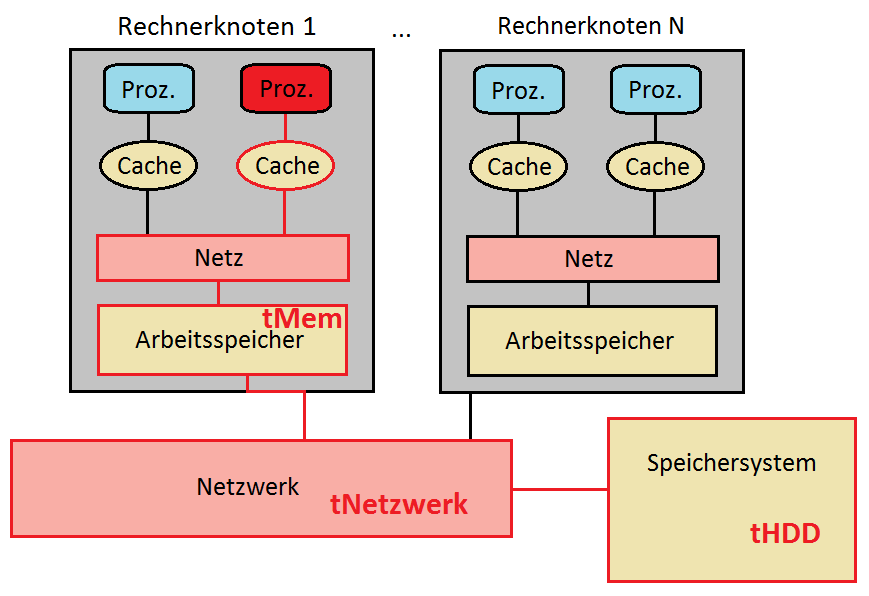
\includegraphics[width=.43\textwidth]{Bilder/rechnerknoten_ea_pfad.png}
	\end{center}
	\caption{E/A-Pfad im System; der rot gekennzeichnete Prozessor macht einen E/A-Zugriff , der Pfad führt entlang der roten Markierung}
	\label{fig:ea_pfad}
\end{figure}

Für einen Schreibzugriff gilt im Wesentlichen ein ähnlicher Ablauf.
Die Daten müssen beim Schreiben eigentlich immer über das Netzwerk auf Festplatte geschrieben werden. Dies ist nur dann nicht der Fall, wenn eine Caching-Strategie wie Write-Back genutzt wird. Dann wird die Datei nur im Hauptspeicher des Rechnerknotens geändert und erst später endgültig auf Festplatte geschrieben.
Der Datenfluss beim Schreiben fließt umgekehrt zu dem des Lesezugriffs.

\subsection{Faktoren der Zugriffszeit}
An allen Stationen des E/A-Pfades gibt es jeweils einen konstanten Anteil der Zugriffszeit und einen Anteil, der von der aufgerufenen Datei abhängt. 
Der Teil der Zugriffszeit, der für jeden Aufruf konstant ist, ist für die Modellierung weniger spannend und sollte bereits durch einfache lineare Modelle darstellbar sein, dieser Teil wird im Folgenden nicht weiter berücksichtigt.
Desweiteren kann es an verschiedenen Stellen zu Verzögerungen durch Wartezeiten (engl. queue times) für die Verarbeitung des E/A-Aufrufs kommen. Dieser Faktor ist nicht anhand des Attribut-Tupels bestimmbar und könnte höchstens durch eine Zeitreihenbetrachtung approximiert werden. Konstanter Verwaltungsaufwand und Wartezeiten können als Latenzzeit zusammengefasst werden. Die Latenz einer Station des E/A-Pfades ist also die Verzögerungszeit, bis die Datenübertragung angelaufen ist.\\
Im Folgenden sollen die Faktoren betrachtet werden, die im Wesentlichen von den bekannten Variablen des Attribut-Tupels abhängen.
Für beide Zugriffsarten ergeben sich die drei beschriebenen Zeitfaktoren tMem, tHDD und tNetzwerk.

\begin{itemize}
	\item Der netzwerkabhängige Teil tNetzwerk ist vom genauen Speicherort der aufgerufenen Datei, sowie der Größe der Datei abhängig. Der Faktor des Speicherorts im E/A-System sollte allerdings eine eher ungeordnete Rolle spielen, zudem sind keine Informationen darüber verfügbar; dieser Faktor wird daher vernachlässigt. 
	Der entscheidende Zeitfaktor entsteht durch die Übertragung der Daten über das Netzwerk. Der Datenfluss über das Netzwerk hängt von dessen Durchsatz ab, dieser sollte nach kurzer Verbindungsaufbauphase konstant sein.
	\item tMem ist am einfachsten zu modellieren, denn der hier auftretende Direktzugriffsspeicher (engl. Random-Access Memory) kennzeichnet sich gerade dadurch, dass der Zugriff auf alle Datenblöcke mit gleichem zeitlichen Aufwand verbunden ist.
	Ansonsten hängt die Zugriffszeit vom Durchsatz des Speichers ab.
	Eigentlich handelt es sich bei tMem um die Zusammensetzung der Zeitanteile von dem Arbeitsspeicher und den Caches. tMem wird im Modell jedoch vom langsamsten Speicher, der angesprochen werden muss, dominiert.
	\item Die Festplatte ist ähnlich komplex wie das Netzwerk. Wie beim Netzwerk ist die Zugriffszeit zum Einen von dem genauen Speicherort der angefragten Datenblöcke und zum Anderen vom Durchsatz der Festplatte abhängig.
	Die Zugriffszeit ist von der zu überwindenden Strecke, vom vorherigen Aufenthaltsort zum Zielort, des Lese-/Schreibkopfes abhängig.
	Diese Strecke hängt dabei mit dem $Delta\text{-}Offset$ zusammen.
	Ein großer Abstand der Zugriffsorte in der Datei sollte auch in einem größeren Abstand auf der Magnetscheibe der Festplatte resultieren.
	Der zeitliche Aufwand zum Überwinden des $Delta\text{-}Offsets$ ist von den Hardwarecharakteristika der Festplatte abhängig. Ansonsten ist die Zugriffszeit linear von dem Durchsatz der Festplatte und der Größe des angefragten Abschnittes abhängig.
\end{itemize}

tMem müsste nach diesem Modell vollständig durch ein lineares Modell dargestellt werden können. Dagegen ist dies für tNetzwerk und tHDD nur bedingt der Fall.
Netzwerk und Festplatte haben einen je nach Zugriffsgröße dominierenden linearen Anteil, jedoch auch einen vom Speicherort abhängigen.
Die Durchsätze von tMem sowie tHDD sind hardwarebedingt von der Art des Zugriffs abhängig, es muss also zwischen Lese- und Schreibzugriffen unterschieden werden.
Dies geschieht über den Operationstyp (OpTyp).

Das Modell für die Ein-/Ausgabe in dieser Arbeit entspricht letztendlich:

\begin{align*}
tGesamt &= tHDD + tNetzwerk + tMem\\
\text{mit}\\
tHDD &= \frac{Zugriffsgrö\text{ß}e}{Festplattendurchsatz(OpTyp)} + Festplattenlatenz(Delta\text{-}Offset) \\
tNetzwerk &= \frac{Zugriffsgrö\text{ß}e}{Netzwerkdurchsatz} + Netzwerklatenz\\
tMem &= \frac{Zugriffsgrö\text{ß}e}{Speicherdurchsatz(OpTyp)} + Speicherlatenz
\end{align*}

Alle Messungen zu Speicheraufrufen mit dem selben Attribut-Tupel hätten nach diesem Modell idealerweise die selbe Laufzeit.

\subsection{E/A-Pfad zur Leistungsvorhersage}
\label{analyse:ea_pfad_zurvorhersage}
Anhand eines kurzen Vorgriffs auf die Messdaten-Exploration kann die Auswirkung des E/A-Pfades auf die Laufzeit der Messungen gezeigt werden.
In Abbildung \ref{fig:pfad_for_vorhersage} ist die Zugriffszeit für E/A-Zugriffe einer Messreihe gezeichnet. Alle Messungen derselben Farbe gehören zum selben Attribut-Tupel, ihre Aufrufparameter sind also gleich.
\begin{figure}
	\begin{center}
		\subfloat{
			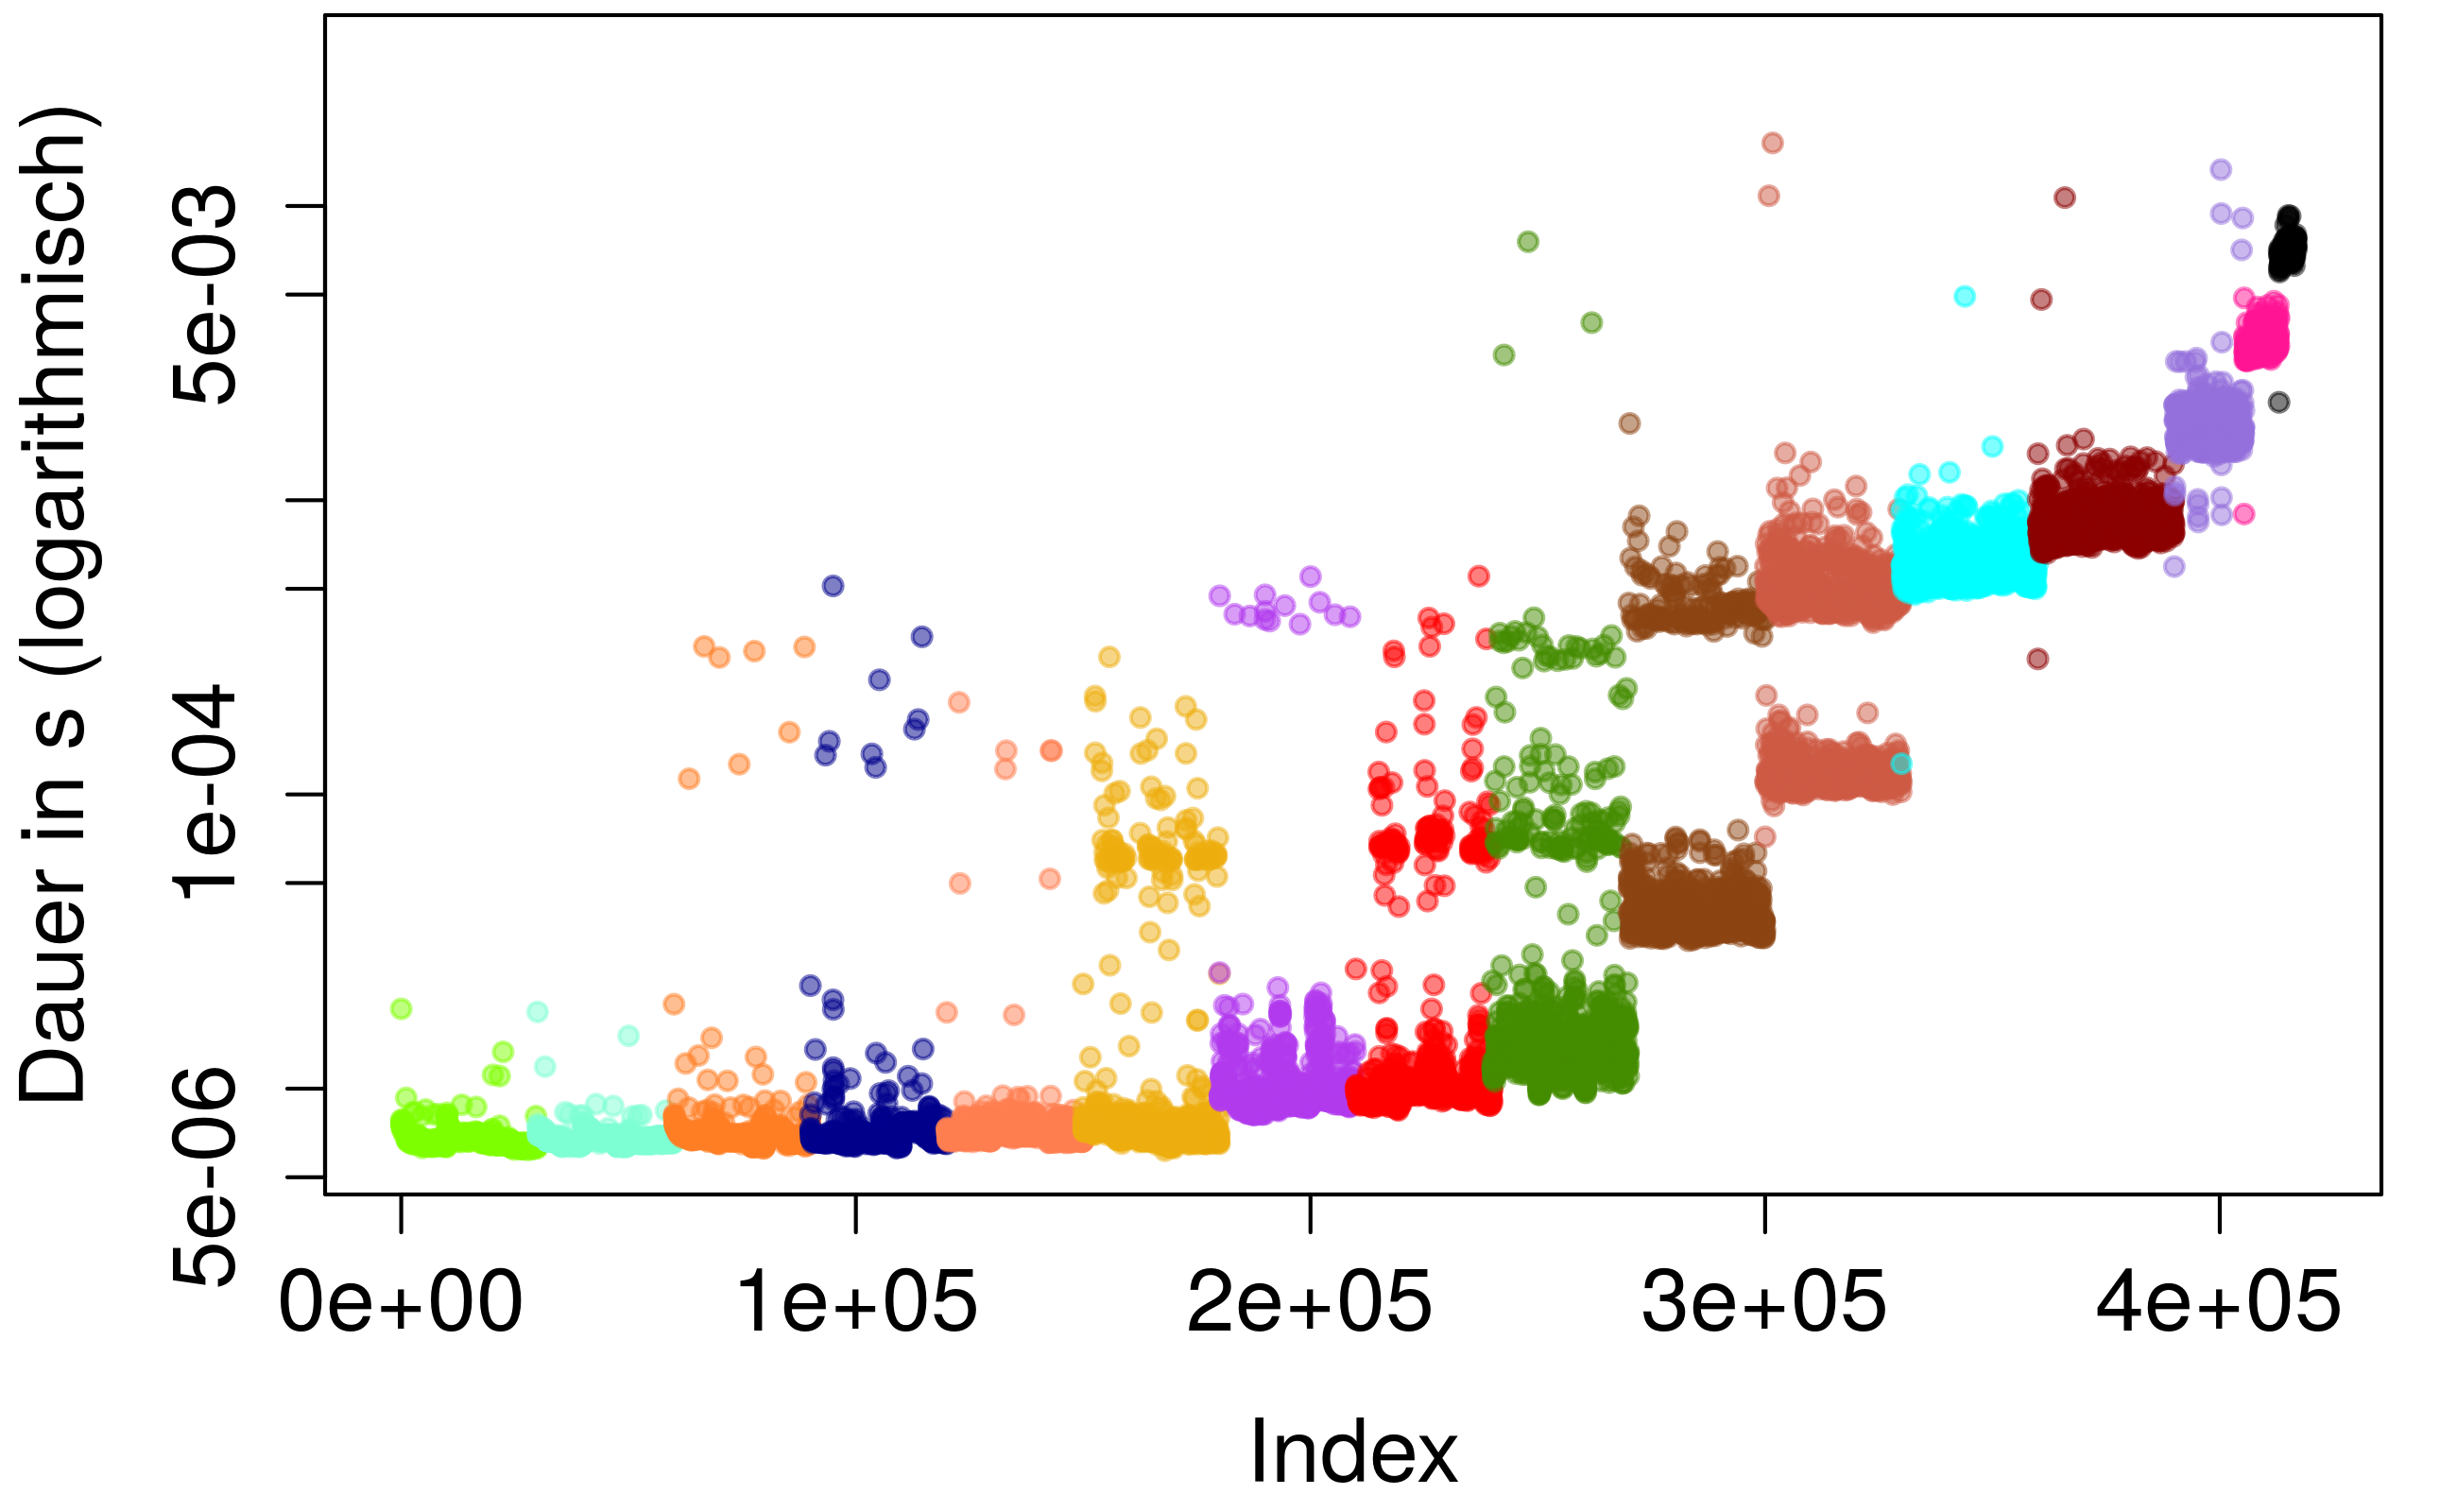
\includegraphics[width=.5\textwidth]{Bilder/Plots/exploration/plot_SizeSorted_log_read_seq.png}
		}
		\caption{Graphische Darstellung der Laufzeiten einer Messreihe mit lesenden E/A-Aufrufen. Jede Farbe repräsentiert eine Zugriffsgröße.}
		\label{fig:pfad_for_vorhersage}
	\end{center}
\end{figure}
In der Abbildung ist gut zu erkennen, dass die Zugriffszeiten in Stufen zunehmen.
Dies liegt einerseits an den in Intervallen ansteigenden Zugriffsgrößen der Messungen, kann aber andererseits auch der Zugehörigkeit der Messung zu einem E/A-Pfad zugesprochen werden.
Die Zugriffszeit eines Pfades wird von der langsamsten Komponente auf dem Weg dominiert.
Dadurch kann ein Sprung in der Laufzeit entstehen sobald sich der Pfad verlängert. Der Pfad verlängert sich, wenn auf eine tiefere Schicht der Speicherhierachie zugegriffen werden muss. Da die tieferen Schichten auch zunehmend langsamer werden, entsteht jedes mal ein Sprung in der Laufzeit.\medskip

In der Abbildung wird auch direkt klar, dass die Annahme fallengelassen werden muss, dass Messungen mit gleichem Attribut-Tupel dieselbe Laufzeit haben. Die Laufzeiten innerhalb von Messreihen zu gleichen Attributen unterscheiden sich teilweise deutlich.
Das ermöglicht allerdings gerade die Abhängigkeit der Laufzeiten vom E/A-Pfad zu sehen.
Wäre die Laufzeit im Wesentlichen nur vom Attribut-Tupel und dem \glqq zufälligen\grqq{} momentanen Systemzustand abhängig, dann sollten die Messungen zum selben Tupel in einer gleichmäßig verteilten Wolke aufzufinden sein.
Die Laufzeiten eines Attribut-Tupels weisen allerdings ein sprunghaftes Verhalten auf. Die dunkelgrünen Punkte sind beispielsweise in drei Gruppen aufgeteilt.
Die roten und violetten Messungen, links neben den dunkelgrünen, weisen ein ähnliches Muster auf, bei den violetten fehlt die mittlere Gruppe.
Die Zugriffsgröße der dunkelgrünen Messungen ist dabei vier mal höher (4KiB zu 16KiB).
Wie lange die Verarbeitung des E/A-Aufrufs dauert, scheint aber im Wesentlichen für die drei Attribut-Tupel gleich zu sein und vor Allem davon abzuhängen, in welcher Stufe sich der zugehörige Punkt der Messung befindet.\medskip

Die zuvor aufgestellte Modellierung kann die Abhängigkeit zwischen E/A-Pfad und Laufzeit nicht wiedergeben. Möglicherweise könnte eine Zeitreihenbetrachtung Hinweise über die Zugehörigkeit einer Messung zu einem Pfad geben. 

Ein perfektes Modell sollte unter Kenntnis des Pfades, den ein E/A-Aufruf nehmen wird, und dem Attribut-Tupel die Dauer des Zugriffs sehr gut vorhersagen können. Wenn das Modell nicht vorhersagen kann welcher Pfad genommen wird, kann es nicht zwischen den Gruppierungen innerhalb der Messungen eines Attribut-Tupels unterscheiden. Die Vorhersagekraft ist damit begrenzt.

\section{Validierung und Metriken}
\label{analyse:valid}
Mit den im Weiteren entwickelten Modellen soll untersucht werden, wie gut es gelingt, den zeitlichen Aufwand für E/A-Aufrufe vorherzusagen. 
Jedes Modell trifft bestimmte Annahmen über das E/A-System und zur Entwicklung einer Instanz des Modells werden bestimmte Informationen benötigt.
Diese benötigten Daten können aus den Messdaten über das System abgeleitet werden.
Ein Teil der Daten wird als Trainingsdatensatz zum Lernen genutzt, die restlichen Daten sind dem Modell unbekannt und bilden den Testdatensatz. Die Vorhersagen der Modelle zum Testdatensatz können dann mit den tatsächlichen Werten verglichen werden. Dies ist die \textbf{Leistungsvorhersage} vom Modell zum System. \medskip

Neben der Vorhersage der Leistung wird in den komplexeren Modellen selbst auch versucht die Quantile 0.1 und 0.9 der Laufzeit vorherzusagen. Der Wert des 0.1 Quantil gibt an, dass 10\% der Laufzeiten die zu einem Attribut-Tupel gemessen wurden langsamer als dieser Wert waren, entsprechend gibt das 0.9 Quantil an, dass nur 10\% der Messungen zu diesem Attribut-Tupel schneller abgearbeitet wurden.
Wenn die schnellsten und langsamsten $10\%$ der Messungen eines Attribut-Sets als Ausreißer bezeichnet werden, können die Modelle mit Hilfe der Vorhersage dieser Quantile eine Klassifikation in Ausreißer und Nicht-Ausreißer machen. Diese Zuordnung wird als \textbf{Ausreißervorhersage} bezeichnet.
Bei den Ausreißern handelt es sich in diesem Kontext nicht um ungültige Messungen, die durch einen fehlerhaften Versuchsaufbau oder durch Fehlkalibrierung von Messinstrumenten entstanden sind. Stattdessen kann es beispielsweise sein, dass das System punktuell sehr ausgelastet war und die Latenzen dadurch ungewöhnlich hoch waren. 
Bei der Ausreißervorhersage wird geprüft, ob das Modell korrekt voraussagen kann, dass die Laufzeit einer E/A-Anfrage zu den Ausreißern gehört. Da es sich bei den Ausreißern nicht um Messfehler handelt ist eine solche Vorhersage prinzipiell möglich, erfordert allerdings eine sehr gute Einsicht ins System.
Man könnte die Ausreißervorhersage auch als Test auf den schwierigsten Daten ansehen. 

Es würde für die Qualität eines Modells sprechen, wenn es sowohl eine gute Leistungsvorhersage, auch eine gute Ausreißervorhersage macht.

\subsubsection{Metriken zur Leistungsvorhersage}
Zur Analyse der Leistungsvorhersage führe ich sechs Fehlermetriken ein.
\begin{itemize}
	\item Der \textit{\textbf{MAE}} (vom englischen \textit{mean absolute error}) ist der arithmetische absolute Fehler gemittelt über alle Vorhersagen.
	\item Der \textit{\textbf{MAPE}} (vom englischen \textit{mean absolute percentage error}) ist der relative \textit{MAE}, also der \textit{MAE} auf dem relativen Fehler der Vorhersage gegenüber der tatsächlichen Laufzeit.\\
\end{itemize}
\textit{MAE} und \textit{MAPE} geben eine Vorstellung davon, welchen Fehler man bei einer Vorhersage erwarten kann.
\begin{itemize}
	\item Um ein Verständnis für die Streuung der Modellabweichungen zu bekommen ist der quadratische relative Fehler gemittelt über alle Vorhersagen \textit{\textbf{MSPE}} (vom englischen \textit{mean square percentage error}) nützlich.
\end{itemize}
	Eine geringe quadratische Abweichung lässt darauf schließen, dass das Modell zuverlässig ist und nicht teilweise gut und für andere Messungen schlecht agiert. Für den selben Zweck sind \textit{Q3} und \textit{Max} nützlich.
\begin{itemize}
	\item \textit{\textbf{Q3}} gibt das obere Quartil des relativen Fehlers über alle Vorhersagen an.
	\item \textit{\textbf{Max}} entspricht dem größten relativen Fehler der vom Modell gemacht wurde.
	\item Der Wert von \textit{\textbf{In-range}} gibt an, wie viele der gemachten Vorhersagen zwischen dem 0.1 und 0.9 Quantil der Laufzeiten aller Messungen eines Attribut-Sets lagen.
	Wenn alle Laufzeiten exakt vorhergesagt werden würden, wäre \textit{In-range} also bei 80\%. An \textit{In-range} lässt sich erkennen, ob ein Modell sehr konservativ vorhersagt, sodass 100\% der prognostizierten Werte zwischen den Quantilen liegen und ob überhaupt sinnvolle Vorhersagen gemacht werden.
\end{itemize}
Zwei zusätzliche Fehlermetriken enthalten weitere nützliche Informationen über die Netze, sodass die Leistung besser eingeordnet werden kann.

\begin{itemize}
	\item \textit{\textbf{Avg-MAPE}} (Avg für \textit{average}) gibt den durchschnittlichen \textit{MAPE}-Wert für 12 Netze an. 
	Aufgrund der zufälligen Initialisierung und der lokalen Konvergenz durch das verwendete Gradientenverfahren sind die neuronalen Netze nicht deterministisch bestimmt.
	Je nachdem mit welchen Gewichten das Netz startet, ist das Ergebnis des Lernalgorithmus besser oder schlechter, um falsche Schlussfolgerungen über die Qualität der Parameter zu verhindern, werden daher jeweils 12 Instanzen mit den gleichen Parametern und Trainingsdaten, aber mit unterschiedlicher Initialisierung, berechnet.
	Anhand des \textit{Avg-MAPE} kann die Auswirkung der lokalen Konvergenz für die jeweiligen Netzstrukturen betrachtet werden.
	\item Zusätzlich wird \textit{\textbf{Train-MAPE}} angegeben. Dies ist der erreichte \textit{MAPE}-Wert des Netzes auf den eigenen Trainingsdaten. Dieser Wert sollte immer besser als der normale \textit{MAPE} sein. Anhand der Differenz zu \textit{MAPE} kann beurteilt werden, wie gut die Trainingsdaten die Testdaten repräsentiert haben.
\end{itemize}

\subsubsection{Metriken zur Ausreißervorhersage}
Zur Evaluierung der Ausreißervorhersage werden weitere Fehlermetriken eingeführt.\medskip

Die ersten Fehlermetriken beziehen sich auf die Vorhersagen der Laufzeit-Quantile. Idealerweise sollte das Modell jeweils einen einheitlichen Wert für die Quantile zu jedem Attribut-Tupel vorhersagen, der möglichst nah am tatsächlichen Wert liegt.
\begin{itemize}
	\item Die arithmetischen Mittelwerte über den relativen Fehlern (\textit{\textbf{Q0.1-MAPE}} und \textit{\textbf{Q0.9-MAPE}}).
	\item Die mittleren quadratischen Abweichungen über die relativen Fehler (\textit{\textbf{Q0.1-MSPE}} und \textit{\textbf{Q0.9-MSPE}}).
\end{itemize}
Zudem werden zwei Metriken einbezogen, die gemeinsam die Klassifikation der Messungen in Ausreißer und Nicht-Ausreißer bewerten können.
\begin{itemize}
	\item \textit{\textbf{TP}} misst den Anteil der korrekt vorhergesagten Ausreißer, dies sind die richtig positiven Zuordnungen (engl. \textit{true positives}). Dieser Wert sollte möglichst hoch sein.
	\item \textit{\textbf{FP}} gibt dagegen die Anzahl Messungen an, die fälschlicherweise als Ausreißer eingestuft wurden (engl. false positives). Dieser Wert sollte gering gehalten werden.
\end{itemize}
Es ist wichtig, sowohl \textit{TP} als auch \textit{FP} zu betrachten. Ein Netz, das einfach alle Messungen als Ausreißer deklariert, würde einen perfekten \textit{TP}-Wert von 100\% erreichen, obwohl mit der Ausreißer-Bestimmung nichts anzufangen ist.

\section{Modellklassen}
\label{analyse:modellklassen}
Modelle unterscheiden sich einerseits anhand der Informationen, die ihnen über die E/A-Messungen zur Verfügung stehen, dies sind ihre Eingabeattribute, und andererseits an der zugrunde liegenden mathematischen Struktur.
Da es sich bei der E/A-Leistungsvorhersage um ein komplexes Problem handelt, steht nicht a priori fest, wie eine passende Modellierung auszusehen hat. 
In dieser Arbeit wurden daher verschiedene Ansätze getestet.

Jedes Modell kann einer Teilmenge von Klassen zugeordnet werden. Jede Klasse entspricht einem bestimmten Ansatz, also einer bestimmten Herangehensweise ans Problem.
Die verschiedenen Modellklassen werden in den folgenden Kapiteln näher erläutert.

\subsection{Referenzmodelle}
Referenzmodelle werden auf einfache Weise mit klassischen mathematischen Methoden mit relativ geringem Rechenaufwand berechnet.
Das Ziel bei den Referenzmodellen ist nicht hauptsächlich die Qualität der Vorhersagen zu untersuchen, sondern verschiedene Ansätze zu erkunden und Vergleichswerte für komplexere Modelle zu liefern.
Einige Referenzmodelle stellen eine untere Schranke für die Vorhersagequalität der aufwendigeren Modelle dar. Andere zeigen auf, was maximal mit einem Ansatz erreichbar ist.
Beispielsweise kann an den Ergebnissen eines Modells, das bloß lineare Zusammenhänge beschreiben kann, untersucht werden, ob die Daten in linearer Weise beschrieben werden können.\medskip

Bei Referenzmodellen wird nicht zwischen Trainings- und Testdaten unterschieden, sie werden immer über die gesamten Messdaten trainiert und ausgewertet.
Eine Separation der Datensätze ist für beide Verwendungszwecke der Referenzmodelle nicht sinnvoll. 
Wenn untersucht werden soll, ob ein lineares Modell die Messdaten beschreiben kann, sollte der gewählte Trainingssatz nicht eingeschränkt werden, ebenso wenn gezeigt werden soll, wie gut ein Konzept maximal sein kann.

\subsection{NN-Modelle}
Das Hauptaugenmerk der Arbeit liegt auf der Anwendung von künstlichen neuronalen Netzen zur Leistungsvorhersage der E/A-Zugriffe. Die Modelle, die auf neuronalen Netzen basieren, werden als NN-Modelle bezeichnet.
Die Erwartungshaltung ist, dass NN-Modelle wesentlich bessere Ergebnisse erzielen, als die Referenzmodelle, die untere Schranken für die Leistung definieren.
Wenn dies nicht der Fall ist, war entweder die Modellierung unzureichend oder die verwendeten Informationen über die Messdaten waren unzureichend für eine gute Beschreibung des E/A-Systems.\medskip

Bei NN-Modellen gibt es die Aufteilung zwischen Trainings- und Testdatensatz.
Sie könnten daher auch in einer realen Anwendungssituation genutzt werden. 
Bei der tatsächlichen Anwendung eines E/A-Leistungsprädiktors wäre es nicht möglich, dass das Modell bereits sämtliche E/A-Aufrufe gesehen hat, deren Laufzeiten es vorhersagen soll.

\subsection{Fehlerklassen-Modelle}
\label{fk-modelle}
Fehlerklassen (\textbf{FK}) werden mit Hilfe der Vorhersagen eines anderen Modells berechnet. Der Fehler (auch Residuum oder Modellabweichung) der Vorhersagen gegenüber den tatsächlichen Laufzeiten der E/A-Aufrufe wird mit dem k-Means-Algorithmus (siehe Kapitel \ref{back_ML}) in 10 Cluster unterteilt.
Jede Cluster-Gruppe entspricht einer Klasse und bekommt eine Nummer. 
Die Klassen repräsentieren unterschiedliche Pfade, die im E/A-System genommen wurden. Dies ist dann der Fall, wenn das Modell, mit dem die Fehlerklassen erstellt wurden, bereits recht gute Vorhersagen macht und somit den \textit{üblichen} E/A-Pfad des Attribut-Tupels richtig bestimmt. 
Ein gutes Modell, das nicht zwischen Fehlerklassen unterscheidet, würde beispielsweise zu den gleichfarbigen Punkten in Abbildung \ref{fig:pfad_for_vorhersage} die mittlere Laufzeit aller zugehörigen Messungen vorhersagen, oder vielleicht allen eine Laufzeit aus der Gruppe mit den meisten Punkten zuordnen. 
Der dabei gemachte Fehler gegenüber den tatsächlichen Laufzeiten ist dann charakteristisch für die Sprünge, die bei den Übergängen der Pfade beobachtet wurden.
Wenn zum Beispiel zu den dunkelgrünen Punkten jeweils ein Wert aus der mittleren Gruppe von Messungen vorhergesagt werden würde, so würde ein sehr kleiner Fehler eine Zugehörigkeit zum dort genommenen E/A-Pfad repräsentieren.
Ein größerer negativer oder positiver Fehler würde darauf hinweisen, dass bei diesem Aufruf ein entsprechend anderer Pfad genommen wurde.\\
Die Schätzung ist, dass das System pro Anwendungsfall etwa 10 verschiedene E/A-Pfade nutzt, daher werden die Messungen in 10 Gruppen aufgeteilt.\medskip

Es muss beachtet werden, dass Modelle, die Fehlerklassen ausnutzen, keine verwendbaren Prädiktoren zur Leistungsvorhersage ergeben.
Die Fehlerklassen müssen ebenso auf den Trainingsdaten wie auch auf den Testdaten berechnet werden, damit die Modelle daraus auf die Laufzeit schließen können.
Für die Zuordnung in Fehlerklassen werden jedoch die Modellabweichungen eines anderen Modells benötigt. Die tatsächlichen Laufzeiten der Testdaten müssen für Modelle mit Fehlerklassen also bekannt sein.\medskip

Die Modelle, die zusätzlich zu den Attribut-Tupeln der Messungen die jeweiligen Fehlerklassen kennen, werden untersucht, um die Aussagekraft von E/A-Pfaden zu analysieren.
Wenn E/A-Pfade charakteristisch für die Zugriffszeiten sind, dann sollten diese Modelle eine wesentlich geringere Modellabweichung aufzeigen als Modelle ohne Fehlerklassen.

Sowohl Referenzmodelle als auch NN-Modelle werden im Folgenden entwickelt und untersucht.
\subsection{Aufbereitung der Trainingsdaten}

Die Eingabedaten der Modelle können auf zwei grundsätzlich verschiedene Weisen aufbereitet werden.
Entweder werden Informationen zu jeder einzelnen Messung eingegeben oder sie werden zunächst als Aggregate zusammengefasst.\medskip

Das Problem ist, dass zu verschiedenen Messungen eines Attribut-Tupels \glqq widersprüchliche\grqq{} Angaben zur Laufzeit gemacht werden. 
Für die Aggregate werden bestimmte Attribute definiert und alle Messungen mit identischen Werten zu allen diesen Attributen werden zusammengefasst.
Der Wert für die Laufzeit eines Aggregats ergibt sich in dieser Arbeit immer als arithmetischer Mittelwert über alle zugehörigen Messungen.
Die Modelle, die nur aggregierte Eingabedaten nutzen, vereinfachen das Problem entsprechend sehr stark. Sie verfolgen den Ansatz, dass es mit den gegebenen Informationen nicht möglich ist, innerhalb eines Attribut-Sets zu differenzieren, sodass verschiedene Messungen eines Sets alle dieselbe Vorhersage zugewiesen bekommen.

Modelle, die Einzelmessungen als Eingabe bekommen, müssen anders mit den \glqq widersprüchlichen\grqq{} Informationen umgehen.
Das Modell muss dann entweder intern die Daten zusammenfassen, um doch die selbe Vorhersage für jede Messung eines Sets zu machen oder es versucht anhand weiterer Informationen über den Systemzustand eine Differenzierung durchzuführen.
Die zweite Lösung entspricht der Zeitreihenbetrachtung.
Modelle, die eine Zeitreihenbetrachtung machen, brauchen die (zeitlich sortierten) Einzelmessungen als Eingabe, da bei der Aggregierung alle zeitabhängigen Informationen verloren gehen.
Sie können dafür versuchen, ein periodisches Systemverhalten zu erkennen und dieses für ihre Vorhersage auszunutzen. So könnte es beispielsweise sein, dass jeder dritte Leseaufruf doppelt so lange wie die vorherigen dauert, weil das E/A-System zunächst einem anderen Prozess Priorität gibt.
Wenn ein solches Verhalten erkannt wird, könnte die Vorhersage durch so ein Modell erheblich verbessert werden.

\section{Untersuchte Modelle}
\label{analyse:modelle}
Bevor die Modelle entwickelt wurden, die in dieser Arbeit untersucht werden sollen, wurden die Messdaten exploriert (siehe \ref{exploration}), um zu verstehen, welche Attribute zu den Messungen interessant sind.
Wenn es darum geht, gute Attribute für die Modelle zu finden, kann die Korrelation des Attributs zu den Laufzeiten der Messungen betrachtet werden.
Die Korrelation ist ein Wert zwischen 0 und 1, und ist ein Maß für den linearen Zusammenhang zweier Variablen. Eine Korrelation von 0 besagt, dass die Information über eine der Variablen keinen linearen Zusammenhang zur Anderen hat.
Bei einer Korrelation von 1 dagegen, kann eine lineare Funktion angegeben werden, aus der sich der Wert der einen Variablen direkt der Wert der Anderen berechnen lässt. Somit ist eine hohe Korrelation zwischen einem Attribut eines E/A-Aufrufs und dessen Laufzeit ein Hinweis darauf, dass dieses Attribut zur Vorhersage der Laufzeit verwendet werden könnte. 
Allerdings wird bei der Korrelation bloß die lineare Abhängigkeit betrachtet, ein komplexerer Zusammenhang zweier Variablen wird dadurch schlecht oder gar nicht repräsentiert.
Abgesehen von der Korrelation war Expertenwissen ausschlaggebend für die Wahl der verwendeten Attribute für jedes Modell.

Ich stelle nun kurz alle Modelle vor, die untersucht wurden. Zunächst gehe ich die Referenzmodelle durch, dann die NN-Modelle.

\subsection{Referenzmodelle}

\begin{itemize}
	\item Das einfachste Modell ist \textit{\textbf{Durchschnitt}} das Modell approximiert alle Laufzeiten mit dem globalen arithmetischen Mittelwert der Laufzeiten.
Da das Modell überhaupt nicht auf die Attribute der betrachteten Messungen eingeht, sollten alle Modelle, die dies tun, bessere Leistungen erbringen. Einem Modell, das diese Informationen ausnutzt und dennoch schlechtere Leistungen erzielt, könnte unterstellt werden, im Wesentlichen zufällige Vorhersagen zu machen.
\textit{Durchschnitt} ist als untere Schranke für alle NN-Modelle gedacht.
	\item Eine ähnliche Methode wie \textit{Durchschnitt} verwendet das Modell \textit{\textbf{Median agg}}. Es berechnet für jedes Attribut-Tupel den Median der Laufzeiten, dieser Wert entspricht dann der Vorhersage des Modells für Messungen zu diesem Attribut-Tupel.
Dieses Modell ist eine Referenz dazu, wie gut die Modellierung eines Modells, das nicht nicht zwischen verschiedenen Messungen zum selben Attribut-Tupel unterscheiden kann, maximal sein kann.
	\item Lineare Regression ist ein einfaches numerisches Verfahren, das eine lineare Funktion berechnet, die den quadratischen Fehler zu den bekannten Messpunkten minimiert (Methode der kleinsten Quadrate).
Die Funktion ist eine Gerade der Form $f(x) = a + b \cdot x$, mit der Verschiebung $a$ und Steigung $b$. Wird die Regression über mehrere Variablen gemacht erhält man Verschiebungen und Steigungen, die sich aus den Komponenten zu jeder Variable zusammensetzen.
Ich probiere drei verschiedene lineare Modelle aus.
\textit{\textbf{LinReg G}} wird nur aus dem Zusammenhang von Zugriffsgröße und Laufzeit berechnet.
\textit{\textbf{LinReg G+D}} enthält auch die Werte zu Delta-Offset und \textit{\textbf{LinReg G+D+O}} berücksichtigt zudem den Operationstyp der Messungen.
Die Modelle können wegen der linearen Form nicht innerhalb eines Attribut-Tupels unterscheiden. Sollte das vermessene E/A-System bereits durch lineare Zusammenhänge in den gemessenen Informationen beschreibbar sein, so sollten diese Modelle gute Ergebnisse zeigen.
\textit{LinReg G} wird einmal mit Einzelmessungen als Eingabe berechnet und einmal mit aggregierten Eingabedaten, dabei wird über alle Attribute des Attribut-Tupels (Zugriffsgröße, Delta-Offset und OpTyp) aggregiert. 
Da die quadratische Abweichung des berechneten linearen Modells zu allen Eingabedaten minimiert wird, findet bei der Einzelmessungs-Eingabe eine Gewichtung nach Häufigkeit des Auftretens eines Attribut-Tupels statt.
	\item Zuletzt gibt es noch zwei Fehlerklassen-Modelle. Die Eingabedaten sind aggregiert nach dem Attribut-Tupel und den Fehlerklassen. 
Sie funktionieren also genauso wie \textit{Median agg}, nur dass die Messungen zusätzlich noch durch ihre Fehlerklasse unterschieden werden. Es wird also der Median für alle Messungen eines Attribut-Tupels berechnet, die zur selben Fehlerklasse gehören.
\textit{\textbf{LinRegFK Median agg}} kennt die Fehlerklassen, die aus der Clusteranalyse der Fehler von \textit{LinReg G} gewonnen wurden, und \textit{\textbf{Tupel1FK Median agg}} modelliert mit Hilfe der Klassen, die aus den Modellabweichungen der besten Instanz von \textit{Tupel1} berechnet wurden.
\end{itemize}

\begin{table}
	\centering
	\scriptsize
	\subfloat{
		\begin{tabular}{|r|p{4.6cm}|p{4.4cm}|p{3.2cm}|}\hline%
			\textbf{Modell} & \textbf{Beschreibung}  & \textbf{Art der Trainingsdaten} & \textbf{Benötigte Attribute zur Vorhersage}\\\hline\hline
			\csvreader[late after line=\\\hline, separator=semicolon]%
			{CSV/zusammenfassung_der_referenz_modelle.csv}{Modell=\Modell, Beschreibung=\Beschreibung, Art=\Art, Attribute = \Attribute}%
			{\Modell & \Beschreibung & \Art & \Attribute}%
		\end{tabular}
	}
	\label{tab:zusammenfasssung_referenz}
	\caption{Kurzbeschreibungen der der Referenzmodelle}
\end{table}

\subsection{NN-Modelle}
Die weiteren Modelle sind NN-Modelle, es handelt sich hierbei um neuronale Netze, die sich anhand der Eingabeattribute unterscheiden.

\begin{itemize}
	\item Das Modell \textit{\textbf{NN-Tupel1 agg}} is analog zu \textit{Median agg}. Das Modell kennt allerdings, so wie alle NN-Modelle, nur einen Ausschnitt der Messdaten.
	Im Gegensatz zum zuvor betrachteten Idealfall muss das Modell die Laufzeiten unbekannter Mess-Attribute interpolieren.
	Der Eingabevektor, den das neuronale Netz zu jedem Aggregat erhält, beinhaltet die Werte zu allen Attributen des Attribut-Tupels, nach diesen Attributen wurden die Trainingsdaten auch aggregiert.
	Das Netz versucht dann also das Tripel $(Zugriffsgr\text{ß}e, Delta\text{-}Abstand, Operationstyp)$ in Relation zum zugehörigen Median der Laufzeiten zu bringen.
	Das Modell muss sich nicht bloß die Mediane der Laufzeiten zu den Attribut-Tupeln \textit{merken}, sondern möglichst gut die Zusammenhänge zwischen den Attribut-Werten und den zugehörigen Laufzeit-Mediane bestimmen, um unbekannte Attribut-Sets sinnvoll vorhersagen zu können.
	\item Ganz ähnlich wie \textit{NN-Tupel1 agg} ist das Modell \textit{\textbf{NN-Tupel1}} aufgebaut. Die Eingabedaten werden allerdings nicht aggregiert.
	Es versucht also direkt das beschriebene Tripel auf die zugehörigen Laufzeiten abzubilden. Es erhält sonst keine weiteren Informationen, sodass es ebenso wenig, wie das aggregierende Modell, zwischen Messungen mit gleichen Attributen unterscheiden kann.
	Es muss dann selbständig einen Mittelwert zu jedem Attribut-Tupel bilden und mit diesem assoziieren.
\end{itemize}
	\begin{figure}
		\centering
		\subfloat[Skizze von Tupel1 agg]{
			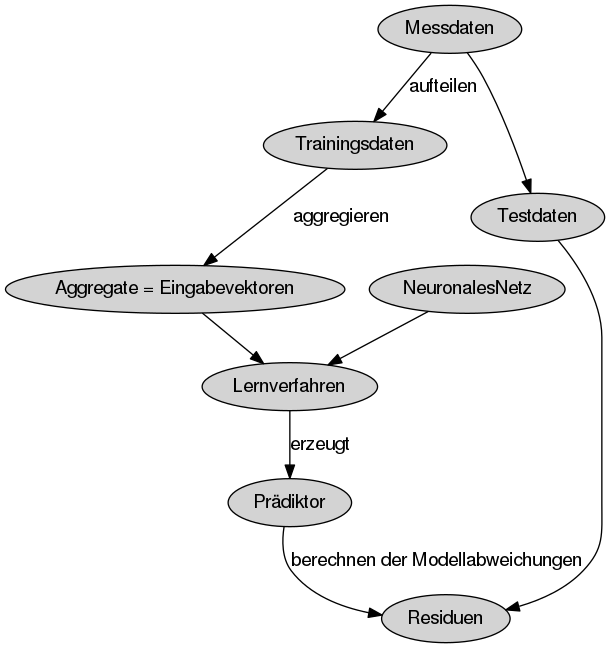
\includegraphics[width=.5\textwidth,height=.5\textwidth]{Dot/tupel1agg.png}
		}
		\subfloat[Skizze von Tupel1]{
			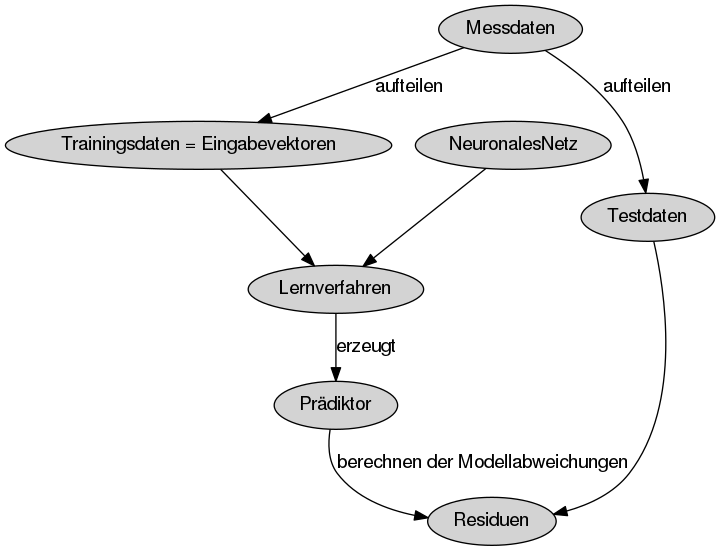
\includegraphics[width=.5\textwidth,height=.5\textwidth]{Dot/tupel1.png}
		}
		\caption{Vergleich der Erstellung und Anwendung von Tupel1 agg (links) und Tupel1(rechts)}
		\label{fig:tupel1vstupel1agg}
	\end{figure} 
\begin{itemize}
	\item \textit{\textbf{NN-Tupel2}} ist das erste Modell, das die zeitliche Reihenfolge der Messungen ausnutzen soll. Das neuronale Netz bekommt nicht nur die Werte zum Attribut-Tupel der Messung, dessen Leistung es vorhersagen soll, sondern auch die zum Attribut-Tupel und die Laufzeit der vorherigen Messung.
	Die Idee hierbei ist, dass anhand des Wissens, wie schnell die letzte E/A-Prozedur bearbeitet werden konnte, eine Aussage über die Nächste getroffen werden kann. Falls das System beispielsweise gerade besonders ausgelastet ist, sollte sich dies an der vergangenen E/A-Leistung niederschlagen.
	Es könnte auch sein, dass das System eine sehr simple Periodizität aufweist. Sodass, nach einer schnellen Bearbeitung eine langsame folgt oder Ähnliches.
	\item Eine tieferliegende Periodizität könnte unter Umständen durch \textit{\textbf{NN-EMA}} für die Vorhersage der Laufzeit ausgenutzt werden. Die Grundlage für dieses Modell bildet die exponentielle Glättung (im englischen \textit{exponentiell moving average} (EMA)), in der Signalverarbeitung ist dies ein Tiefpassfilter mit unendlicher Impulsantwort.
	Mit dessen Funktionswert kann ein Einblick in den generellen Trend der Zeitreihe gewährt werden, da temporäre Spitzen geglättet werden.
	Die Idee dieses Verfahrens ist, dass der kommende Zeitreihenwert im wesentlichen von den direkten Vorgängern beeinflusst wird, in einem geringeren Maße jedoch auch von weiter zurückliegenden Messungen.
	In dem hier betrachteten Fall könnte das beispielsweise bedeuten, dass ein E/A-Aufruf gemacht wurde, der Speicherblöcke angefragt hat, die über das Netzwerk zum Rechnerknoten geholt werden müssen, da das Netzwerk jedoch gerade durch andere Zugriffe ausgelastet ist, hat der Aufruf ungewöhnlich lange gedauert. Nun werden ein paar Aufrufe innerhalb des eigenen Arbeitsspeichers gemacht, die eine normale Laufzeit aufweisen. Über den aktuellen Wert der exponentiellen Glättung besteht noch eine Erinnerung an das langsame Verhalten vor einigen E/A-Aufrufen, sodass ein erneuter Aufruf über das weiterhin ausgelasteten Netzwerk eventuell genauer gemacht werden könnte.
	Um die Auslastung des E/A-Systems sinnvoll wiederzugeben wird der Durchsatz der Messungen für die exponentielle Glättung genutzt. Der Durchsatz berechnet sich als $Durchsatz =  \frac{Zugriffsgrö\text{ß}e}{Laufzeit}/$.
	
	Karardzic definiert den EMA rekursiv \cite{kantardzic2011data} (S. 40):
	\begin{align*}
	EMA(i,m) &= p \cdot t(i)+(1-p) \cdot EMA(i-1,m-1)\\
	EMA(i,1) &= t(i)
	\end{align*}
	Dabei ist $p$ also die Gewichtung für den direkten Vorgängerwert und $1-p$ die Gewichtung für alle vergangenen Werte, $i$ ist der aktuelle Messwert und es werden die letzten $m$ Messungen berücksichtigt. Nummerieren wir alle Messungen von 1 bis $n$ durch und berücksichtigen immer alle bisherigen Messungen, also $i = m$, so sind die ersten Werte:
	\begin{align*}
	EMA(1,1) &= t(1)\\
	EMA(2,2) &=  p \cdot t(2)+(1-p) \cdot t(1)\\
	EMA(3,3) &=  p \cdot t(3)+(1-p) \cdot (p \cdot t(2)+(1-p) \cdot t(1))
	\end{align*}
	Der Eingabevektor des neuronalen Netzes \textit{NN-EMA} enthält alle Attribute des Attribut-Tupels, zusätzlich erhält es den EMA mit $p=0.5$ der vergangenen Durchsätze.
	\item Abschließend gibt es, parallel zu den trivialen Modellen, auch zwei NN-Modelle, die mit Fehlerklassen arbeiten.
	Die beiden Modelle bekommen das Attribut-Tupel der Messungen und zudem deren Fehlerklasse als Eingabeattribute.
	\textit{\textbf{NN-LinRegFK}} mit den Fehlerklassen die aus den Residuen des Referenzmodells \textit{LinReg G} berechnet wurden und \textit{\textbf{NN-Tupel1FK}} mit den Fehlerklassen, die aus den Ergebnissen der \textit{Tupel1} Instanz mit geringstem MSPE-Wert berechnet wurden.
\end{itemize}

\begin{figure}
	\centering
	%\subfloat[Skizze von NN-LinRegFK]{
	%	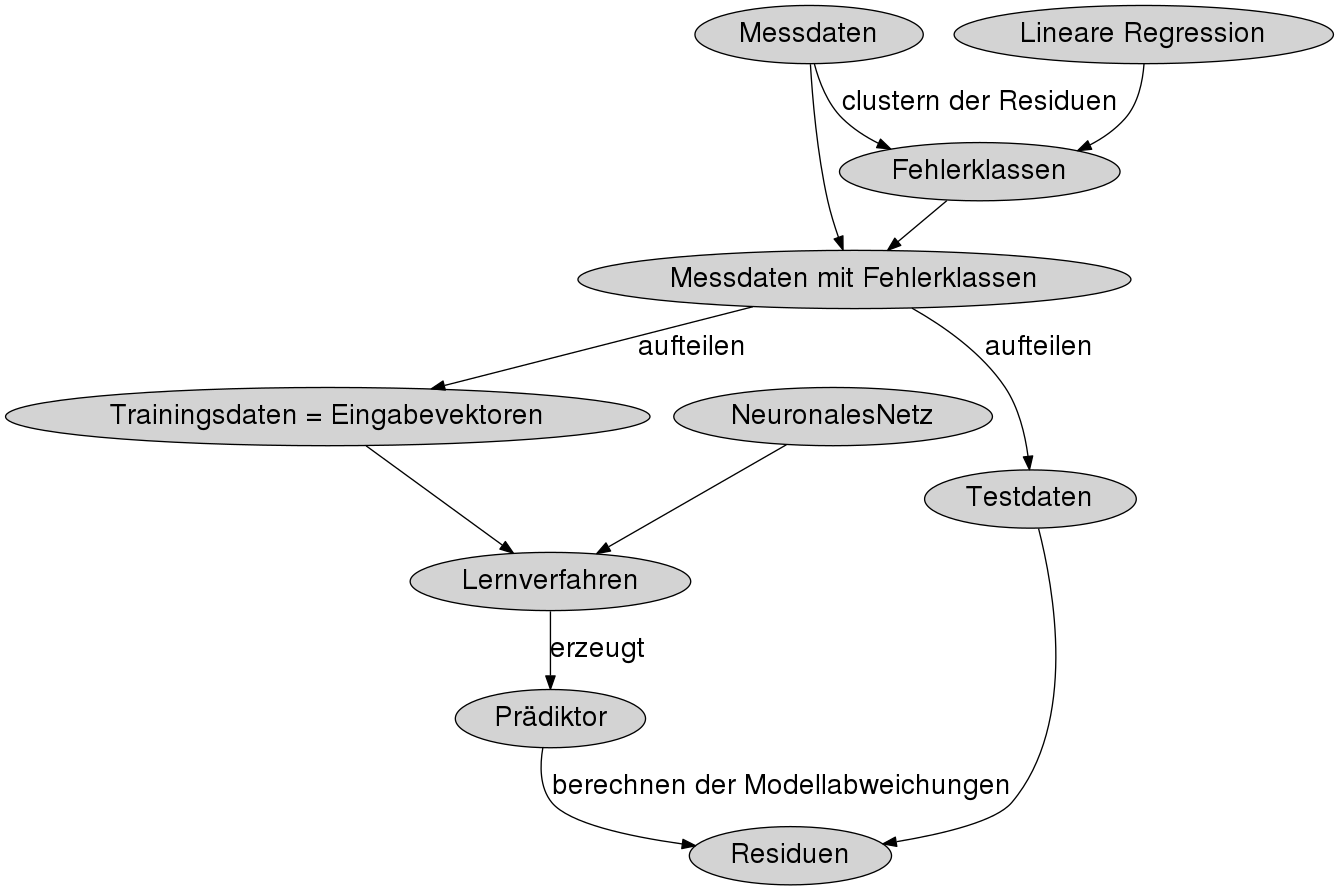
\includegraphics[height=.6\textwidth]{Dot/linregfk.png}
	%}\\
	\subfloat[Skizze von NN-Tupel1FK]{
		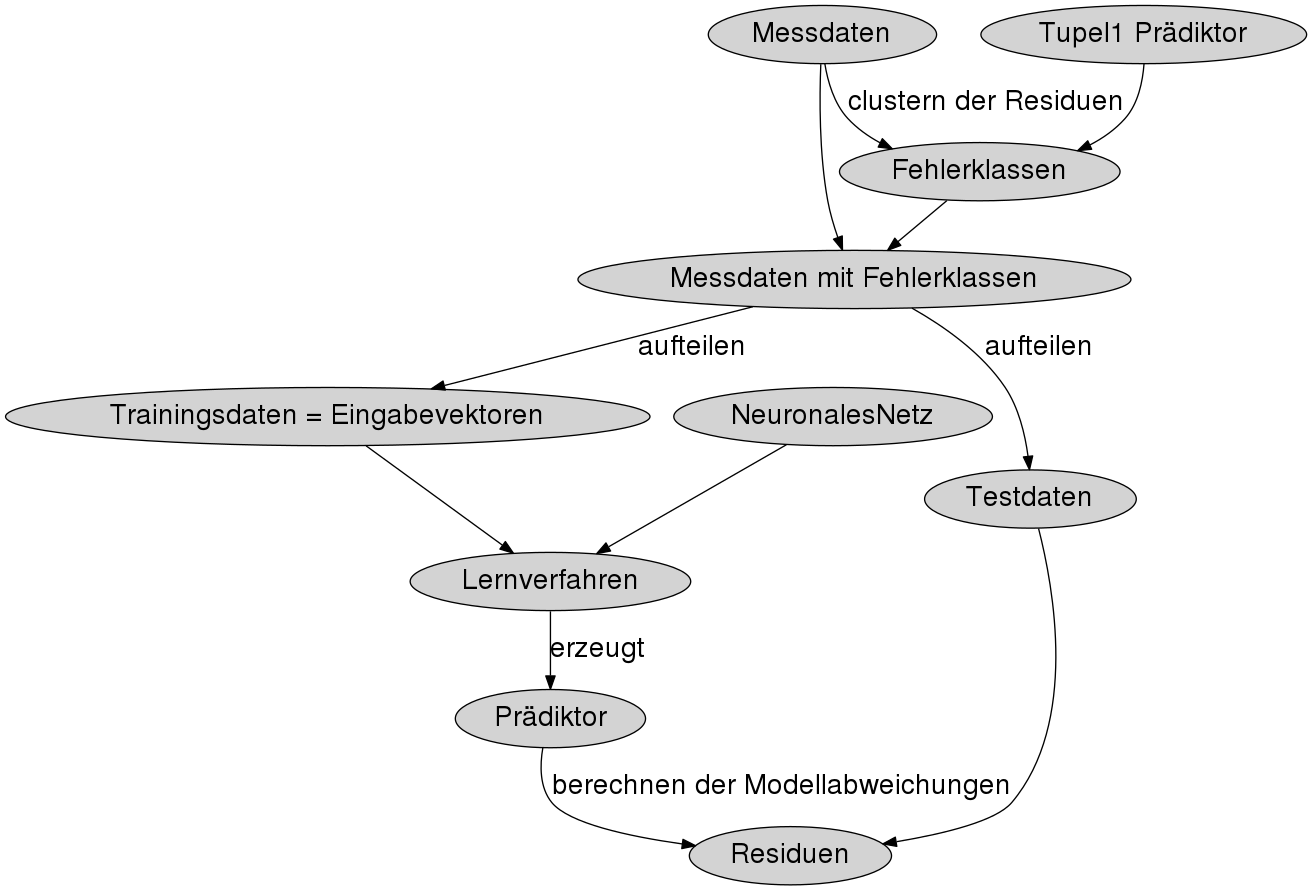
\includegraphics[height=.6\textwidth]{Dot/tupel1fk.png}
	}
	\caption{Erstellung und Anwendung von NN-Tupel1FK. NN-LinRegFK nutzt statt dem aus Tupel1 gewonnenen Prädiktor lineare Regression zum Erstellen der Fehlerklassen.}
	\label{fig:linregfkvstupel1fk}
\end{figure}

\begin{table}
	\centering
	\scriptsize
	\subfloat{
		\begin{tabular}{|r|p{4.6cm}|p{4.4cm}|p{3.2cm}|}\hline%
			\textbf{Modell} & \textbf{Beschreibung}  & \textbf{Art der Trainingsdaten} & \textbf{Attribute des Eingabevektors}\\\hline\hline
			\csvreader[late after line=\\\hline, separator=semicolon]%
			{CSV/zusammenfassung_der_NN_modelle.csv}{Modell=\Modell, Beschreibung=\Beschreibung, Art=\Art, Attribute = \Attribute}%
			{\Modell & \Beschreibung & \Art & \Attribute}%
		\end{tabular}
	}
	\label{tab:zusammenfasssung_nn}
	\caption{Kurzbeschreibungen der der NN-Modelle. Diese basieren auf neuronalen Netzen und bilden den Eingabevektor auf die Laufzeit ab.}
\end{table}

\section{Parametrisierung von NN-Modellen}
\label{parametrisierung}
Für die Referenzmodellen ist die Berechnung eindeutig definiert.
Bei den NN-Modellen hingegen müssen zunächst die Parameter der verwendeten neuronalen Netze festgelegt werden. 
Während manche Parameter durch Heuristiken oder nach einigen Testdurchläufen schnell ermittelt werden können, sind andere stark abhängig von den tatsächlichen Trainingsdaten, der Anzahl Datenpunkte und den verwendeten Attributen. 

Als Funktion zur Fehlerrückführung wird in allen Netzen eine resilente Backpropagation genutzt. Verwendet wurde der \textit{Rprop+} (\textit{resilent backpropagation with weightbacktracking}) Algorithmus.  (vgl. \cite{gunther2010neuralnet} S. 32).
Im Unterschied zur normalen Backpropagation wird jedes Gewicht mit einer individuellen Lernrate verändert. Die Anpassung der Gewichte zu den Verbindungen geschieht bei diesem Algorithmus nicht über die Größe des Gradienten in der Fehlerfunktion, sondern bloß über das Vorzeichen des Gradienten zusammen mit der Lernrate.
Durch das merken der Gewichte der vergangenen Iteration kann der letzte Aktualisierungsschritt rückgängig gemacht werden (der englische Fachausdruck dazu ist weightbacktracking). Dies wird genutzt, falls das Minimum der Fehlerfunktion überschritten wurde, dann wird stattdessen ein kleinerer Schritt durchgeführt (vgl. \cite{gunther2010neuralnet} S. 32).

Als Fehlerfunktion bietet sich die mittlere quadratische Abweichung der Ausgabe des Netzes zur idealen Ausgabe an.
Für die Aktivierungsfunktion wird die logistische Funktion verwendet, die sich durch einen weicheren Übergang als die Stufenfunktion zwischen minimalen und maximalen Wert auszeichnet, sodass ein Neuron nicht ganz oder gar nicht feuert, sondern auch etwas dazwischen möglich ist. Bei der logistischen Funktion handelt es sich um eine Sigmoidfunktion, sie hat daher eine wohldefinierte Ableitung, was für die Fehlerrückführung benötigt wird. 

Die Werte der übrigen Parameter müssen durch systematisches Durchsuchen des Parameterraums für jedes Modell herausgefunden werden. Dabei handelt es sich um die Anzahl verdeckter Schichten und die Anzahl Neuronen pro Schicht, sowie dem Schwellenwert für die partiellen Ableitungen des Fehlergradienten, der als Haltekriterium für den Lernalgorithmus verwendet wird.
Dabei werden zunächst Netze in einer großen Spannweite der Parameterwerte berechnet, um die Parameter dann immer weiter einzugrenzen, wenn sich ein Trend für besonders gute Ergebnisse in einem Wertebereich ergibt.

\paragraph{Zusammenfassung:}
\textit{
Es wurde in diesem Kapitel dargestellt, wie das Problem der Leistungsvorhersage von Ein- und Ausgabe, in dieser Arbeit angegangen werden soll.
Zunächst wurde erläutert welche Informationen über das E/A-System bekannt sind. Dann ist darauf eingegangen worden, wie die Verarbeitung von E/A-Aufrufen modelliert werden kann. Dabei ist die Vermutung aufgestellt worden, dass die Laufzeit essentiell durch den E/A-Pfad bestimmt ist. 
Weiterhin wurden die verschiedenen Modelle vorgestellt, die bei der Evaluierung untersucht werden sollen und die Validierung, sowie Berechnung, dieser beschrieben.
Nachdem im nächsten Kapitel die Implementierung der Analyse angerissen wird, werden in Kapitel \ref{eval} die hier vorgestellten Modelle anhand von Messdaten evaluiert.
}


\chapter{Implementierung}
\textit{%
In diesem Kapitel soll kurz auf ein paar wesentliche Punkte eingegangen werden, die bei der Umsetzung der Analyse von Bedeutung sind.
}
\bigskip

\subsubsection{Verwendete Programmiersprache und Bibliotheken}
Die Skripte zur Aufbereitung der Messdaten, Berechnung der Modelle, sowie zur Auswertung der Ergebnisse wurden mit der Programmiersprache R geschrieben.
Die neuronalen Netze wurden mit dem \textit{neuralnet} Paket \cite{gunther2010neuralnet} berechnet. Der Lernvorgang der Netze ist recht aufwendig und kann mehrere Stunden in Anspruch nehmen.
Desweiteren sind die idealen Parameterwerte nicht bekannt, sodass viele Netze berechnet werden müssen, um den Parameterraum zu durchsuchen.
Der Zeitaufwand kann durch die parallele Berechnung mehrerer Netze deutlich reduziert werden, sodass die Mehrkernprozessoren der Rechner ausgenutzt werden.
Eine Code-Parallelisierung kann für ein System mit gemeinsamen Arbeitsspeicher am einfachsten durch die Parallelisierung von Schleifen erreicht werden. Dafür verwende ich die Pakete \textit{doParallel} und \textit{foreach} \cite{weston2014getting}.
Die \textit{EMA}-Werte für \textit{NN-EMA} werden mit dem Paket \textit{TTR} berechnet.

\subsubsection{Implementationsdetails}
Um die neuronalen Netze am effektivsten zu Nutzen, sollten die Eingabewerte normiert werden. Ansonsten würde einem Attribut mit hoher Werte-Domäne sonst eine größere Bedeutung vom Gradientienverfahren beigemessen, als einem Attribut mit niederwertiger Domäne. 
Ich normiere daher alle Eingabeattribute auf den Wertebereich 0 bis 1.\medskip

Bei der Exploration der Daten wurde festgestellt, dass es viele Messungen mit sehr kleiner Laufzeit gibt.
Bei der Fehlerminimierung des Lernalgorithmus besteht daher die Gefahr, dass der Fehler für die wenigen langen Laufzeiten bevorzugt verringert wird, da hier das größte Optimierungspotential liegt. Gleiches gilt für die Zugriffsgrößen.
Deswegen werden Laufzeit und Größe zunächst logarithmiert bevor sie normiert werden.
Die Ergebnisse der neuronalen Netze müssen mit passenden Umkehrfunktionen ihrer Vorverarbeitung entsprechend wieder in die ursprünglichen Wertebereiche zurückgeführt werden, um die Fehlermetriken zu bestimmen.\medskip

Da der Algorithmus der die neuronalen Netze berechnet nur ein Haltekriterium hat, das von der Konvergenz der Gewichte abhängt, kann es beliebig lange bis zur Termination dauern.
Um nicht viel Zeit mit der Berechnung von Netzen mit ungeeigneten Parametern zu verbringen, wird daher eine maximale Grenze für die Iterationen des Lernalgorithmus gesetzt. Diese ist zunächst groß gewählt, wenn sich zeigt, dass die besten Netze eines Modells bereits mit weniger Iterationen auskommen, kann eine geringere Grenze gesetzt werden.

\paragraph{Zusammenfassung:}
\textit{
	Nachdem die wichtigsten Details der Implemetierung beschrieben wurden, wird im folgenden Kapitel die Evaluierung der zuvor vorgestellten Analyse durchgeführt.
}

\chapter{Evaluierung}
\label{eval}
\textit{%
	In der Evaluierung sollen die zuvor beschriebenen Modelle in der Umsetzung auf ein reales System untersucht werden.
	Zunächst wird in Abschnitt \ref{eval:testsystem} kurz der untersuchte Hochleistungsrechner vorgestellt.	
	Unterkapitel \ref{eval:benchmark} beschreibt im Detail, welche Messungen auf dem System durchgeführt wurden.
	Die erhaltenen Messdaten werden in Unterkapitel \ref{eval:exploration} genauer betrachtet. Die gewonnenen Informationen können bereits dabei helfen das E/A-System besser zu verstehen.
	In Unterkapitel \ref{eval:fk_analyse} werden die generierten Fehlerklassen genauer analysiert.
	Und abschließend werden in Kapitel \ref{eval:leistungsvorhersage} die Leistungsvorhersagen der verschiedenen Modelle anhand der in Abschnitt \ref{analyse:valid} eingeführten Fehlermetriken und durch die Betrachtung der Verteilung der Modellabweichungen analysiert.
}
\bigskip

\section{Testsystem, Mistral}
\label{eval:testsystem}
Als Testsystem für alle Messungen, die in dieser Arbeit untersucht werden, wurde der Hochleistungsrechner Mistral vom Deutschen Klimarechenzentrum (DKRZ) genutzt.
Mistral befindet sich in der derzeit aktuellen Publikation vom November 2015 auf Platz 64 der von der TOP500-Organisation geführten Liste der schnellsten Supercomputer der Welt.
Das System besteht aus über 1500 Knoten, die jeweils mit zwei Intel E5-2680v3 bestückt sind, diese laufen mit einer Taktfrequenz von 2.5GHz und haben jeweils 30MiB L3 Cache.
Das Speichersystem des Rechners läuft mit dem parallelen und verteilten Dateisystem Lustre.
Es bietet 30 Petabyte Speicherkapazität und eine Speicherbandbreite von 300 GiB/s. Die Messungen wurden während einer üblichen Belastungssituation des Systems durchgeführt, sodass Schwankungen in der Nutzung des E/A-Systems durch andere Nutzer die Messungen beeinflusst haben können.

\section{Aufbau der Benchmark-Tests}
\label{eval:benchmark}
Das Testsystem wird durch eine Reihe von Experimenten untersucht.
Mit Hilfe der daraus erhaltenen Messdaten können die vorgestellten Modelle aus Kapitel \ref{analyse:modelle} entwickelt und anschließend getestet werden.
Um die Stärken und Schwächen der Modelle gut untersuchen zu können, wird ein systematischer Ansatz für die Experimente gewählt.\medskip

Es werden vier verschiedene Experimente durchgeführt, sie repräsentieren zwei unterschiedliche Anwendungsfälle.
Bei allen Tests wurde die Datei, auf die sich die E/A-Anfragen beziehen, zunächst einmal eingelesen. Das System hat die Datei also bereits geladen, die Daten könnten also gecached sein.
Die Testdatei ist allerdings 10GiB groß und passt daher nicht komplett in den Arbeitsspeicher, sodass Zugriffe zu einigen E/A-Anfragen über das Netzwerk auf die Festplatte mit der Datei gehen müssen.
Das genutzte Speicherlayout ist ein \textit{off0}-Layout, das bedeutet, dass die gelesenen Daten von Position 0 des verwendeten Puffers im Arbeitsspeichers ausgelesen bzw. ausgeschrieben werden.
Die Unterscheidung der beiden Anwendungsfälle wird bei der Art des Dateizugriffs gemacht.
Im einem Fall wurde ein sequentieller Zugriff (\textit{seq}) auf die Datei gewählt, im anderen ein zufälliger (\textit{rnd}).
Beim sequentiellen Layout werden die E/A-Operationen jeweils hintereinander auf der Datei ausgeführt. Beispielsweise liest der erste Aufruf die ersten 16KiB, der nächste die darauf folgenden 16KiB.
Dagegen wird beim randomisierten Layout auf eine beliebige Position der Datei zugegriffen.
Beide Anwendungsfälle werden einmal mit lesenden (\textit{R} für read) und einmal mit schreibenden (\textit{W} für write) E/A-Operationen getestet.
Die sich ergebenden Datensätze werden entsprechend als \textit{cached-off0-seq-R}, \textit{cached-off0-seq-W}, sowie \textit{cached-off0-rnd-R} und \textit{cached-off0-rnd-W} bezeichnet.
Die Zugriffsgrößen variieren jeweils von 1B bis 16MiB (im Detail: 1B, 4B, 16B, 64B, 256B, 1KiB, 4KiB, 8KiB, 16KiB, 64KiB, 256KiB, 512KiB, 1MiB, 2MiB, 4MiB, 8MiB und 16MiB).
Zu jeder Größe werden drei Messreihen mit je 10000 Messungen durchgeführt.
Beim sequentiellen Fall werden allerdings nur so viele Aufrufe hintereinander gemessen, bis über das Ende der Datei hinaus zugegriffen werden würde.
Diese Beschränkung trifft für die Messreihen mit Zugriffsgrößen ab 2MiB ein. 16MiB werden im sequentiellen Fall entsprechend nur 640 mal pro Messreihe verwendet, 8MiB 1280 mal, 4MiB 2560 mal und 2MiB 5120 mal.\medskip

Zwischen zwei Messreihen besteht kein Zusammenhang, sodass zeitliche Abhängigkeiten, wie eine bestimmte Periodizität, nur innerhalb einer Messreihe bestehen können.  
Unter der Bezeichnung \textit{cached-off0-seq} ist die Verkettung der beiden Datensätze \textit{cached-off0-seq-R} und \textit{cached-off0-seq-W} zu verstehen. Gleiches gilt für \textit{cached-off0-rnd}.
Da alle Messungen die Eigenschaften \textit{cached} und \textit{off0} aufweisen, werden die Daten verkürzt als SEQ-R, SEQ-W, RND-R und RND-W bzw. SEQ und RND für die zusammengefassten Datensätze bezeichnet. 

\section{Exploration der Daten}
\label{eval:exploration}
Zunächst werde ich die vier Datensätze genauer betrachten. Dazu eignet es sich einige Übersichtsinformationen über sie zu sammeln.
In der Tabelle \ref{tab:meta} sind für alle vier Datensätze zu den drei Attributen Dauer, Zugriffsgröße und Delta-Offset der minimale Wert, der Wert des ersten Quartils, der Median, das arithmetische Mittel, der Wert des dritten Quartils und der maximale Wert angegeben. Zusätzlich sind in Tabelle \ref{tab:korrealtionen} zu Zugriffsgröße, Delta-Offset und OpTyp die Korrelationen gegenüber der Zugriffsdauer angegeben.\medskip

Die Korrelation zwischen Delta-Offset und Laufzeit ist für die Datensätze mit sequentiellen Zugriffen nicht berechenbar. Dies liegt daran, dass der Delta-Offset dort durchgehend 0 beträgt, das ist gerade das Kennzeichen des sequentiellen Zugriffs.
Das Attribut OpTyp kann nur sinnvoll über der Vereinigung von SEQ-R
und SEQ-W bzw. RND-R und RND-W betrachtet werden, da der Operationstyp auf den einzelnen Datensätzen immer gleich ist.

\begin{table}
	\centering
	\scriptsize
	\subfloat[Übersichtsinformationen zu SEQ-R]{
		\begin{tabular}{|r|r|r|r|r|r|r|}\hline%
			Attribut & Min.  & 1. Quartil & Median & Arith. Mittel & 3. Quartil & Max. \\\hline\hline
			\csvreader[late after line=\\\hline]%
			{CSV/exploration/data_summary_read_seq.csv}{Attribut=\Attribut,Min=\Min,Quartil1=\L, Median = \Median, Mittel = \Mittel,Quartil3 = \Q, Max = \Max, Korrelation = \Korrelation}%
			{\Attribut & \Min & \L & \Median & \Mittel & \Q & \Max}%
		\end{tabular}
	}\\
	\subfloat[Übersichtsinformationen zu SEQ-W]{
		\begin{tabular}{|r|r|r|r|r|r|r|}\hline%
			Attribut & Min.  & 1. Quartil & Median & Arith. Mittel & 3. Quartil & Max. \\\hline\hline
			\csvreader[late after line=\\\hline]%
			{CSV/exploration/data_summary_write_seq.csv}{Attribut=\Attribut,Min=\Min,Quartil1=\L, Median = \Median, Mittel = \Mittel,Quartil3 = \Q, Max = \Max, Korrelation = \Korrelation}%
			{\Attribut & \Min & \L & \Median & \Mittel & \Q & \Max}%
		\end{tabular}
	}\\
	\subfloat[Übersichtsinformationen zu RND-R]{
		\begin{tabular}{|r|r|r|r|r|r|r|}\hline%
			Attribut & Min.  & 1. Quartil & Median & Arith. Mittel & 3. Quartil & Max. \\\hline\hline
			\csvreader[late after line=\\\hline]%
			{CSV/exploration/data_summary_read_rnd.csv}{Attribut=\Attribut,Min=\Min,Quartil1=\L, Median = \Median, Mittel = \Mittel,Quartil3 = \Q, Max = \Max, Korrelation = \Korrelation}%
			{\Attribut & \Min & \L & \Median & \Mittel & \Q & \Max}%
		\end{tabular}
	}\\
	\subfloat[Übersichtsinformationen zu RND-W]{
		\begin{tabular}{|r|r|r|r|r|r|r|}\hline%
			Attribut & Min.  & 1. Quartil & Median & Arith. Mittel & 3. Quartil & Max. \\\hline\hline
			\csvreader[late after line=\\\hline]%
			{CSV/exploration/data_summary_write_rnd.csv}{Attribut=\Attribut,Min=\Min,Quartil1=\L, Median = \Median, Mittel = \Mittel,Quartil3 = \Q, Max = \Max, Korrelation = \Korrelation}%
			{\Attribut & \Min & \L & \Median & \Mittel & \Q & \Max}%
		\end{tabular}
	}
	\caption{Metainformationen über die Datensätze}
	\label{tab:meta}
\end{table}
\medskip

Wie das Modell zur Laufzeit in Kapitel \ref{analyse:ea_modell} postuliert hat ist die Korrelation zwischen Zugriffsgröße und Laufzeit sehr stark.
Die wesentlich größere Korrelation bei sequentiellen Datensatz spricht für einen erfolgreichen Einsatz von Caching-Strategien, wie der Read-Ahead-Einstellung.
Die geringe Korrelation zwischen Zugriffszeit und Delta-Offset auf RND kann zwei Ursachen haben: Entweder ist die Abhängigkeit der Attribute wirklich sehr gering oder er lässt sich nicht durch einen linearen Zusammenhang über den gesamte Datensatz ausdrücken. 
Die zweite Erklärung trifft gerade für OpTyp zu. 
Das kann bereits beim Vergleich der Mediane und arithmetischen Mittelwerte zwischen SEQ-R und SEQ-W bzw. RND-R und RND-W erkannt werden.
Obwohl bei den beiden Experimenten mit sequentiellen Zugriffen die exakt gleichen Zugriffe gemacht wurden, ist das arithmetische Mittel der Zugriffszeiten auf SEQ-W etwa 13\% und der Median etwa 65\% höher, die errechnete Korrelation liegt dagegen nur bei 1.8\%. Zwischen RND-R und RND-W ergibt sich ein ähnliches Bild.
Um dies noch genauer zu untersuchen werden die arithmetischen Mittelwerte der Zugriffszeiten auf SEQ-R und SEQ-W für einzelne Zugriffsgrößen miteinander verglichen.
Die mittlere Zugriffsdauer für 16MiB liegt im sequentiellen Fall für lesende Zugriffe bei 14.09 Millisekunden und für schreibende bei 16.96 Millisekunden, das Lesen geht also etwa 17\% schneller.
Für die Zugriffsgröße von einem 4KiB ergibt sich mit einer Zugriffszeit von 0.0154 Millisekunden beim Schreiben gegenüber 0.0139 Millisekunden für das Schreiben eine etwa 10\% längere Laufzeit beim Lesen.

\begin{table}
	\scriptsize
	\makebox[\textwidth][c]{
		\subfloat{
			\begin{tabular}{|r|r|r|r|r|r|r|}\hline%
				Attribut & cached-off0-seq-R  & cached-off0-seq-W & cached-off0-rnd-R & cached-off0-rnd-W & cached-off0-seq & cached-off0-rnd\\\hline\hline
				\csvreader[late after line=\\\hline]%
				{CSV/exploration/data_summary_korrelationen.csv}{Attribut=\Attribut,seqr=\seqr,seqw=\seqw, rndr = \rndr, rndw = \rndw,seq = \seq, rnd = \rnd}%
				{\Attribut & \seqr & \seqw & \rndr & \rndw & \seq &\rnd}%
			\end{tabular}
		}
		\caption{Korrealtionen der Attribute zur Zugriffsdauer auf den verschiedenen Datensätzen}
		\label{tab:korrealtionen}
	}
\end{table}

\subsubsection{Darstellung der Messungen}
Nachdem nun ein grobes Verständnis für die vorliegenden Messdaten erlangt worden ist, folgt eine Betrachtung der tatsächlichen Messungen in Zeitreihe.
Eine Zeitreihe, also eine zeitlich abhängige Folge von Messungen, existiert zu jeder Messreihe.
Bei der Betrachtung der Übersichtsinformationen wurde festgestellt, dass die Zugriffsgröße sehr stark mit der Laufzeit einer Messung korreliert.
In den Graphen in Abbildung \ref{Laufzeiten_Zeitreihe} sind die Messungen der verschiedenen Datensätze daher nach Zugriffsgröße sortiert dargestellt. Die drei Messreihen zu jeder Größe werden direkt hintereinander abgebildet. Auf diese Weise werden die Graphen bei der Evaluierung der Modelle auch dargestellt werden.
Die Korrelation der beiden Attribut Zugriffsgröße und Laufzeit ist deutlich erkennbar, die Laufzeiten nehmen im Mittel zu. Doch es ist auch zu erkennen, insbesondere bei RND-R, dass die Laufzeiten aufgrund der Streuung von weiteren Faktoren abhängen müssen.\medskip

Wenn nicht anders angegeben wird in allen Graphen nur jeder 25te Datenpunkt gezeichnet, um es etwas übersichtlicher zu machen.
Zudem werden alle Punkte halbtransparent dargestellt, sodass überdeckte Schichten und Häufungspunkte erkannt werden können.
In Zeitreihen Abbildungen werden die obersten 1\%, also die langsamsten Datenpunkte, abgeschnitten, um den wesentlichen Teil der Punkte besser erkennen zu können.
Oft ist eine logarithmische Darstellung der Y-Achse hilfreich, damit zwischen den Messungen einer Zugriffsgröße unterschieden werden kann. 
\begin{figure}
	\subfloat[Messungen in Zeitreihe zu SEQ-R]{
		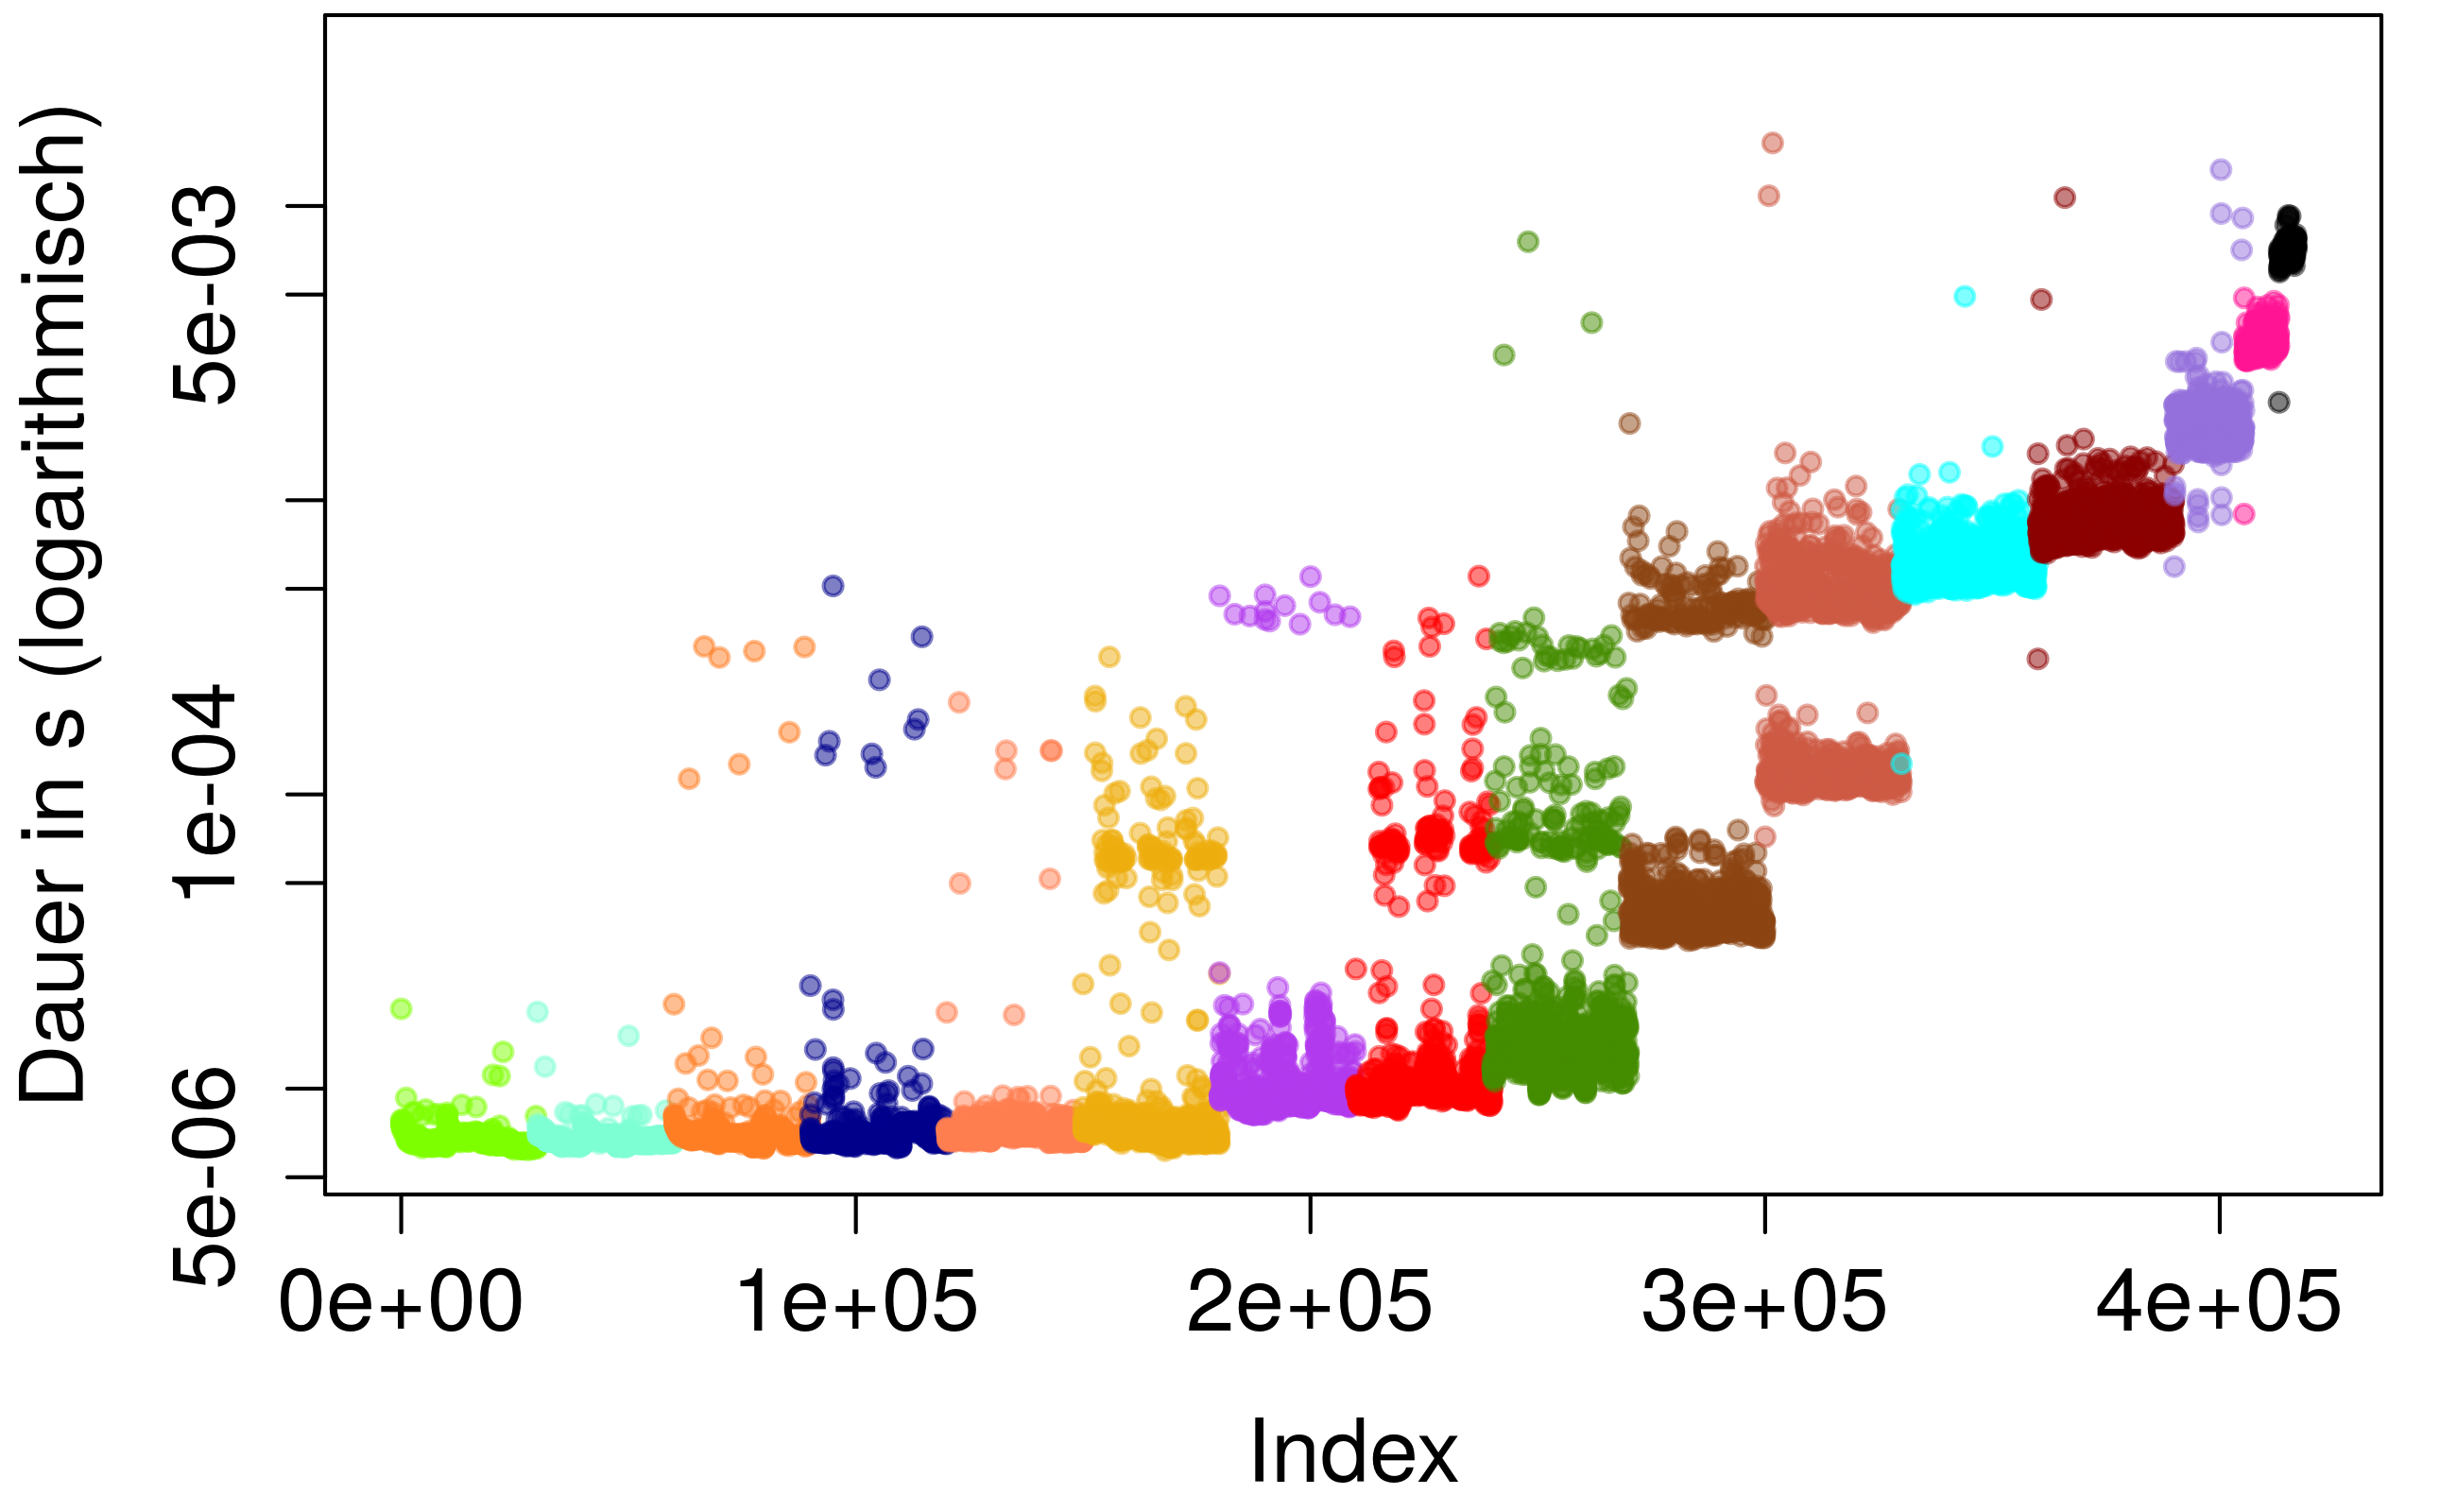
\includegraphics[width=.5\textwidth]{Bilder/Plots/exploration/plot_SizeSorted_log_read_seq.png}
	}
	\hfill
	\subfloat[Messungen in Zeitreihe zu SEQ-W]{
		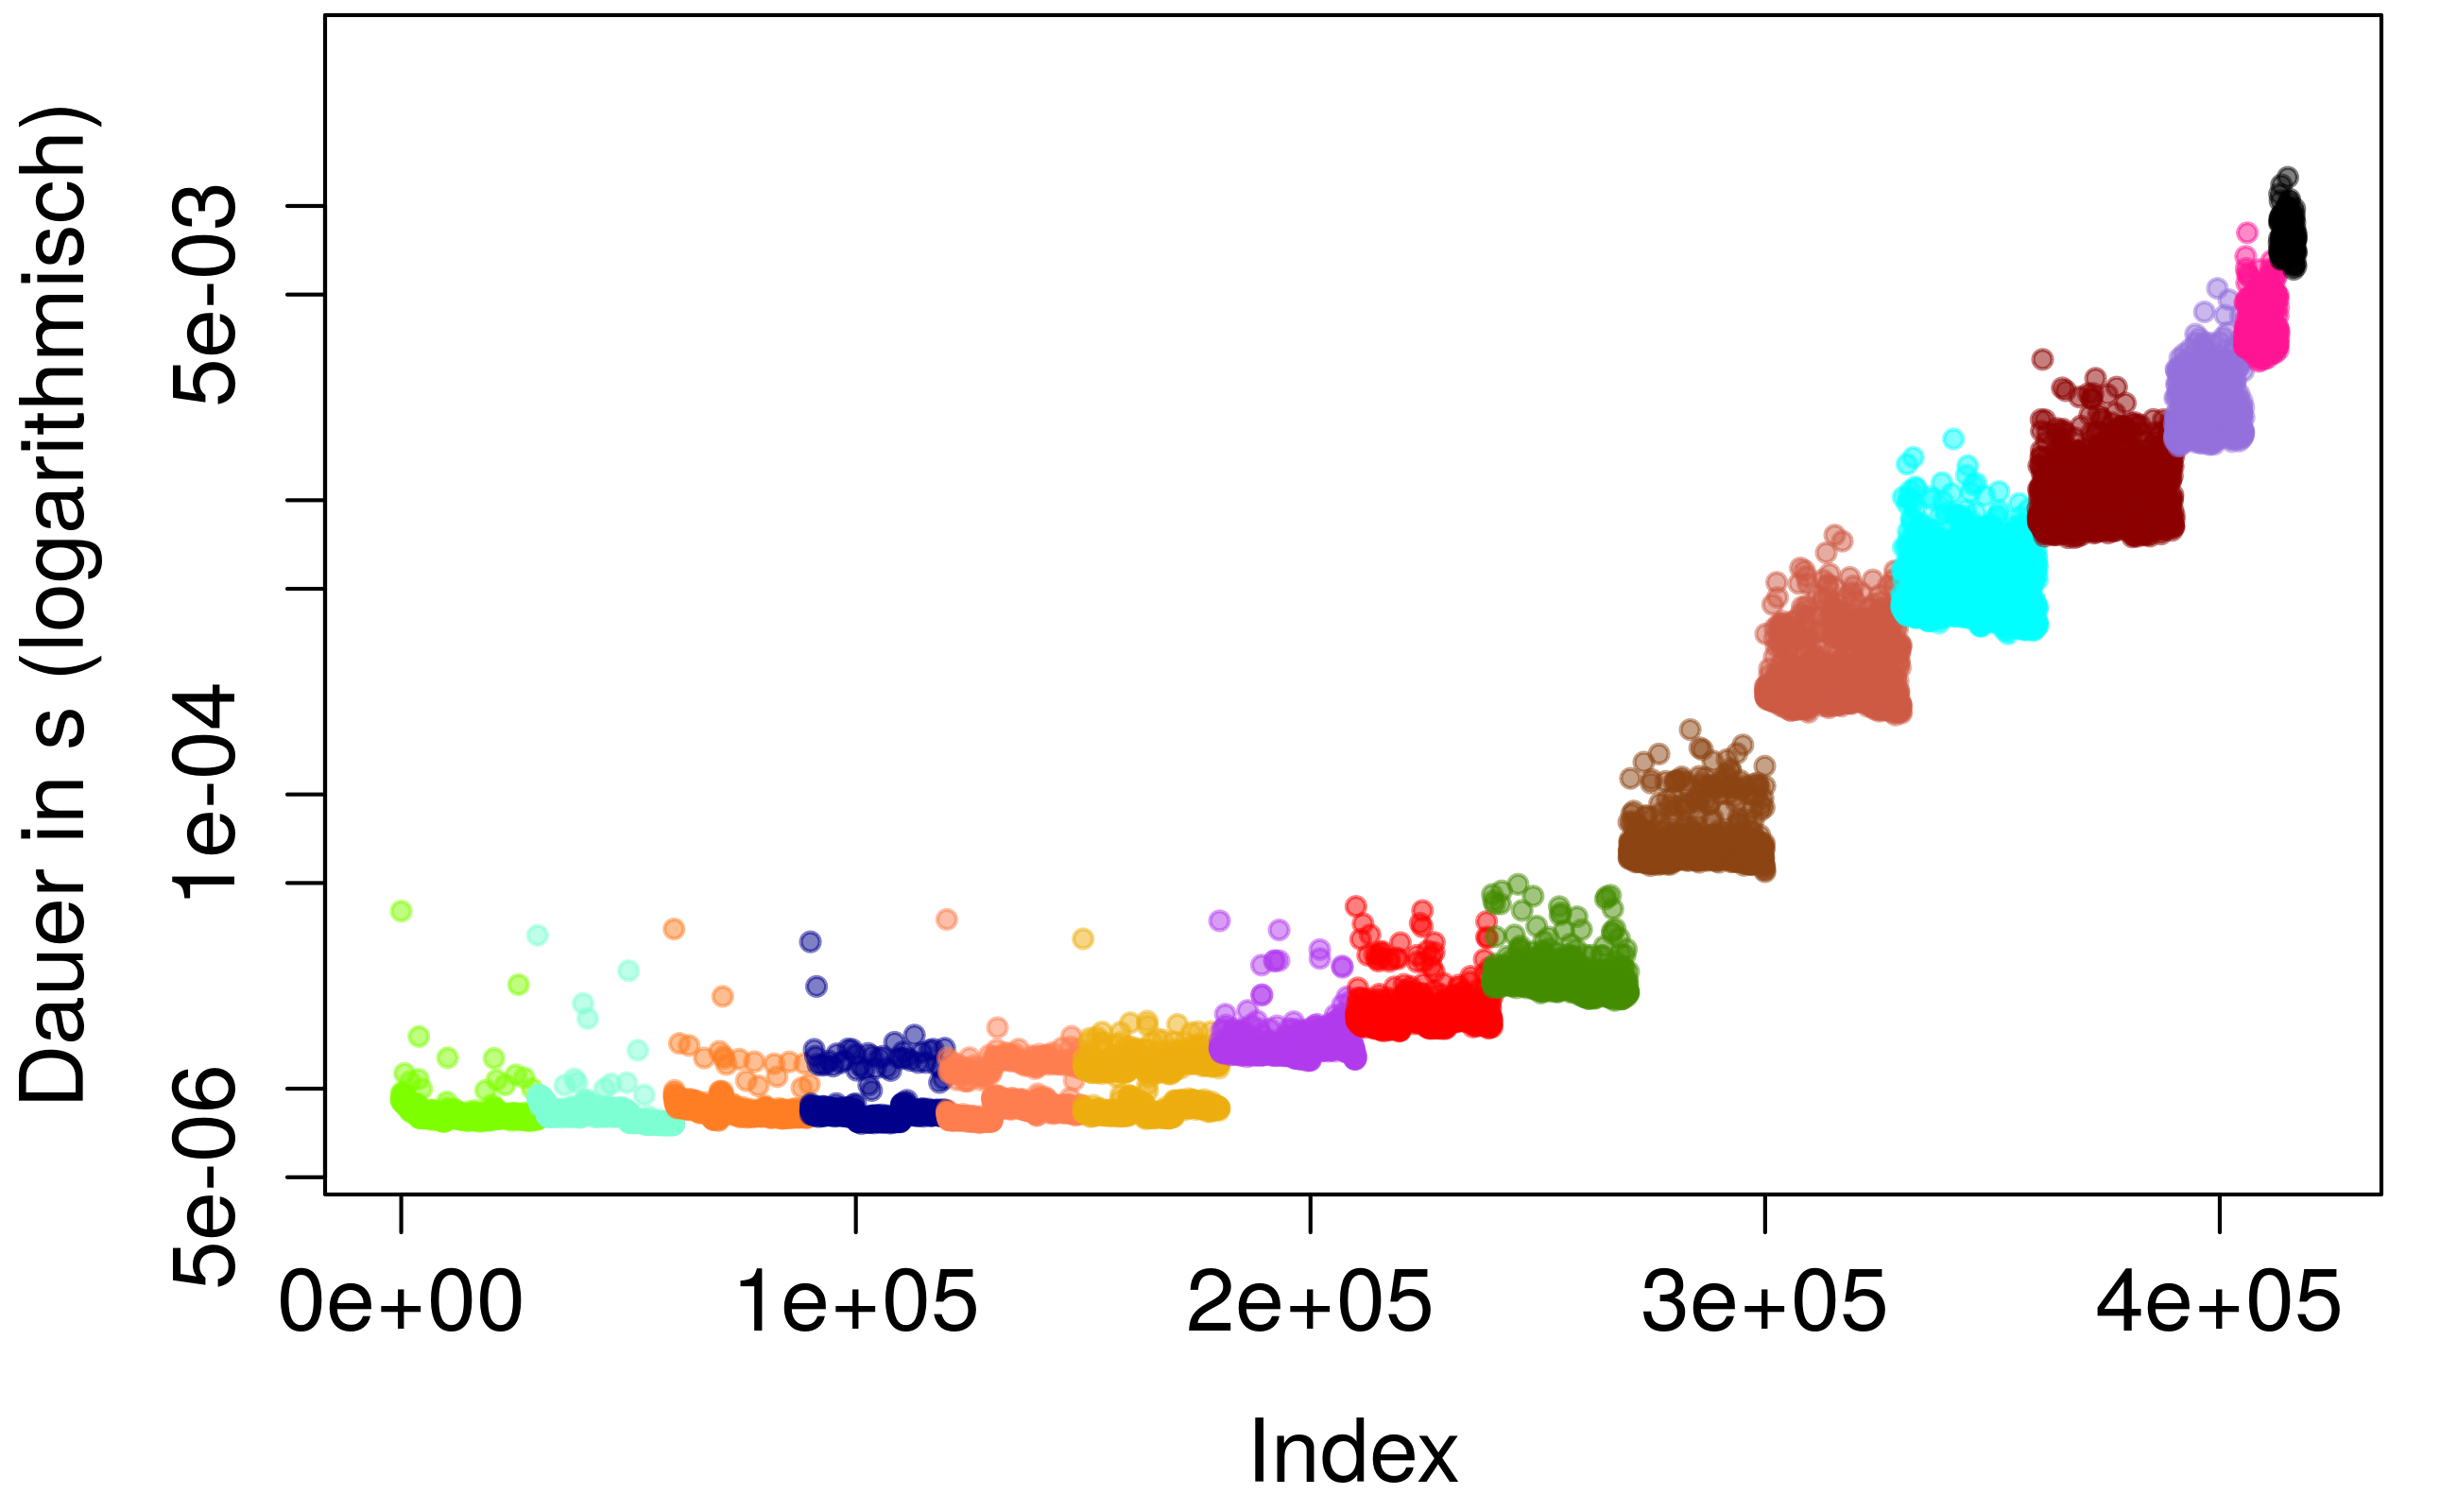
\includegraphics[width=.5\textwidth]{Bilder/Plots/exploration/plot_SizeSorted_log_write_seq.png}
	}\\
	\subfloat[Messungen in Zeitreihe zu RND-R]{
		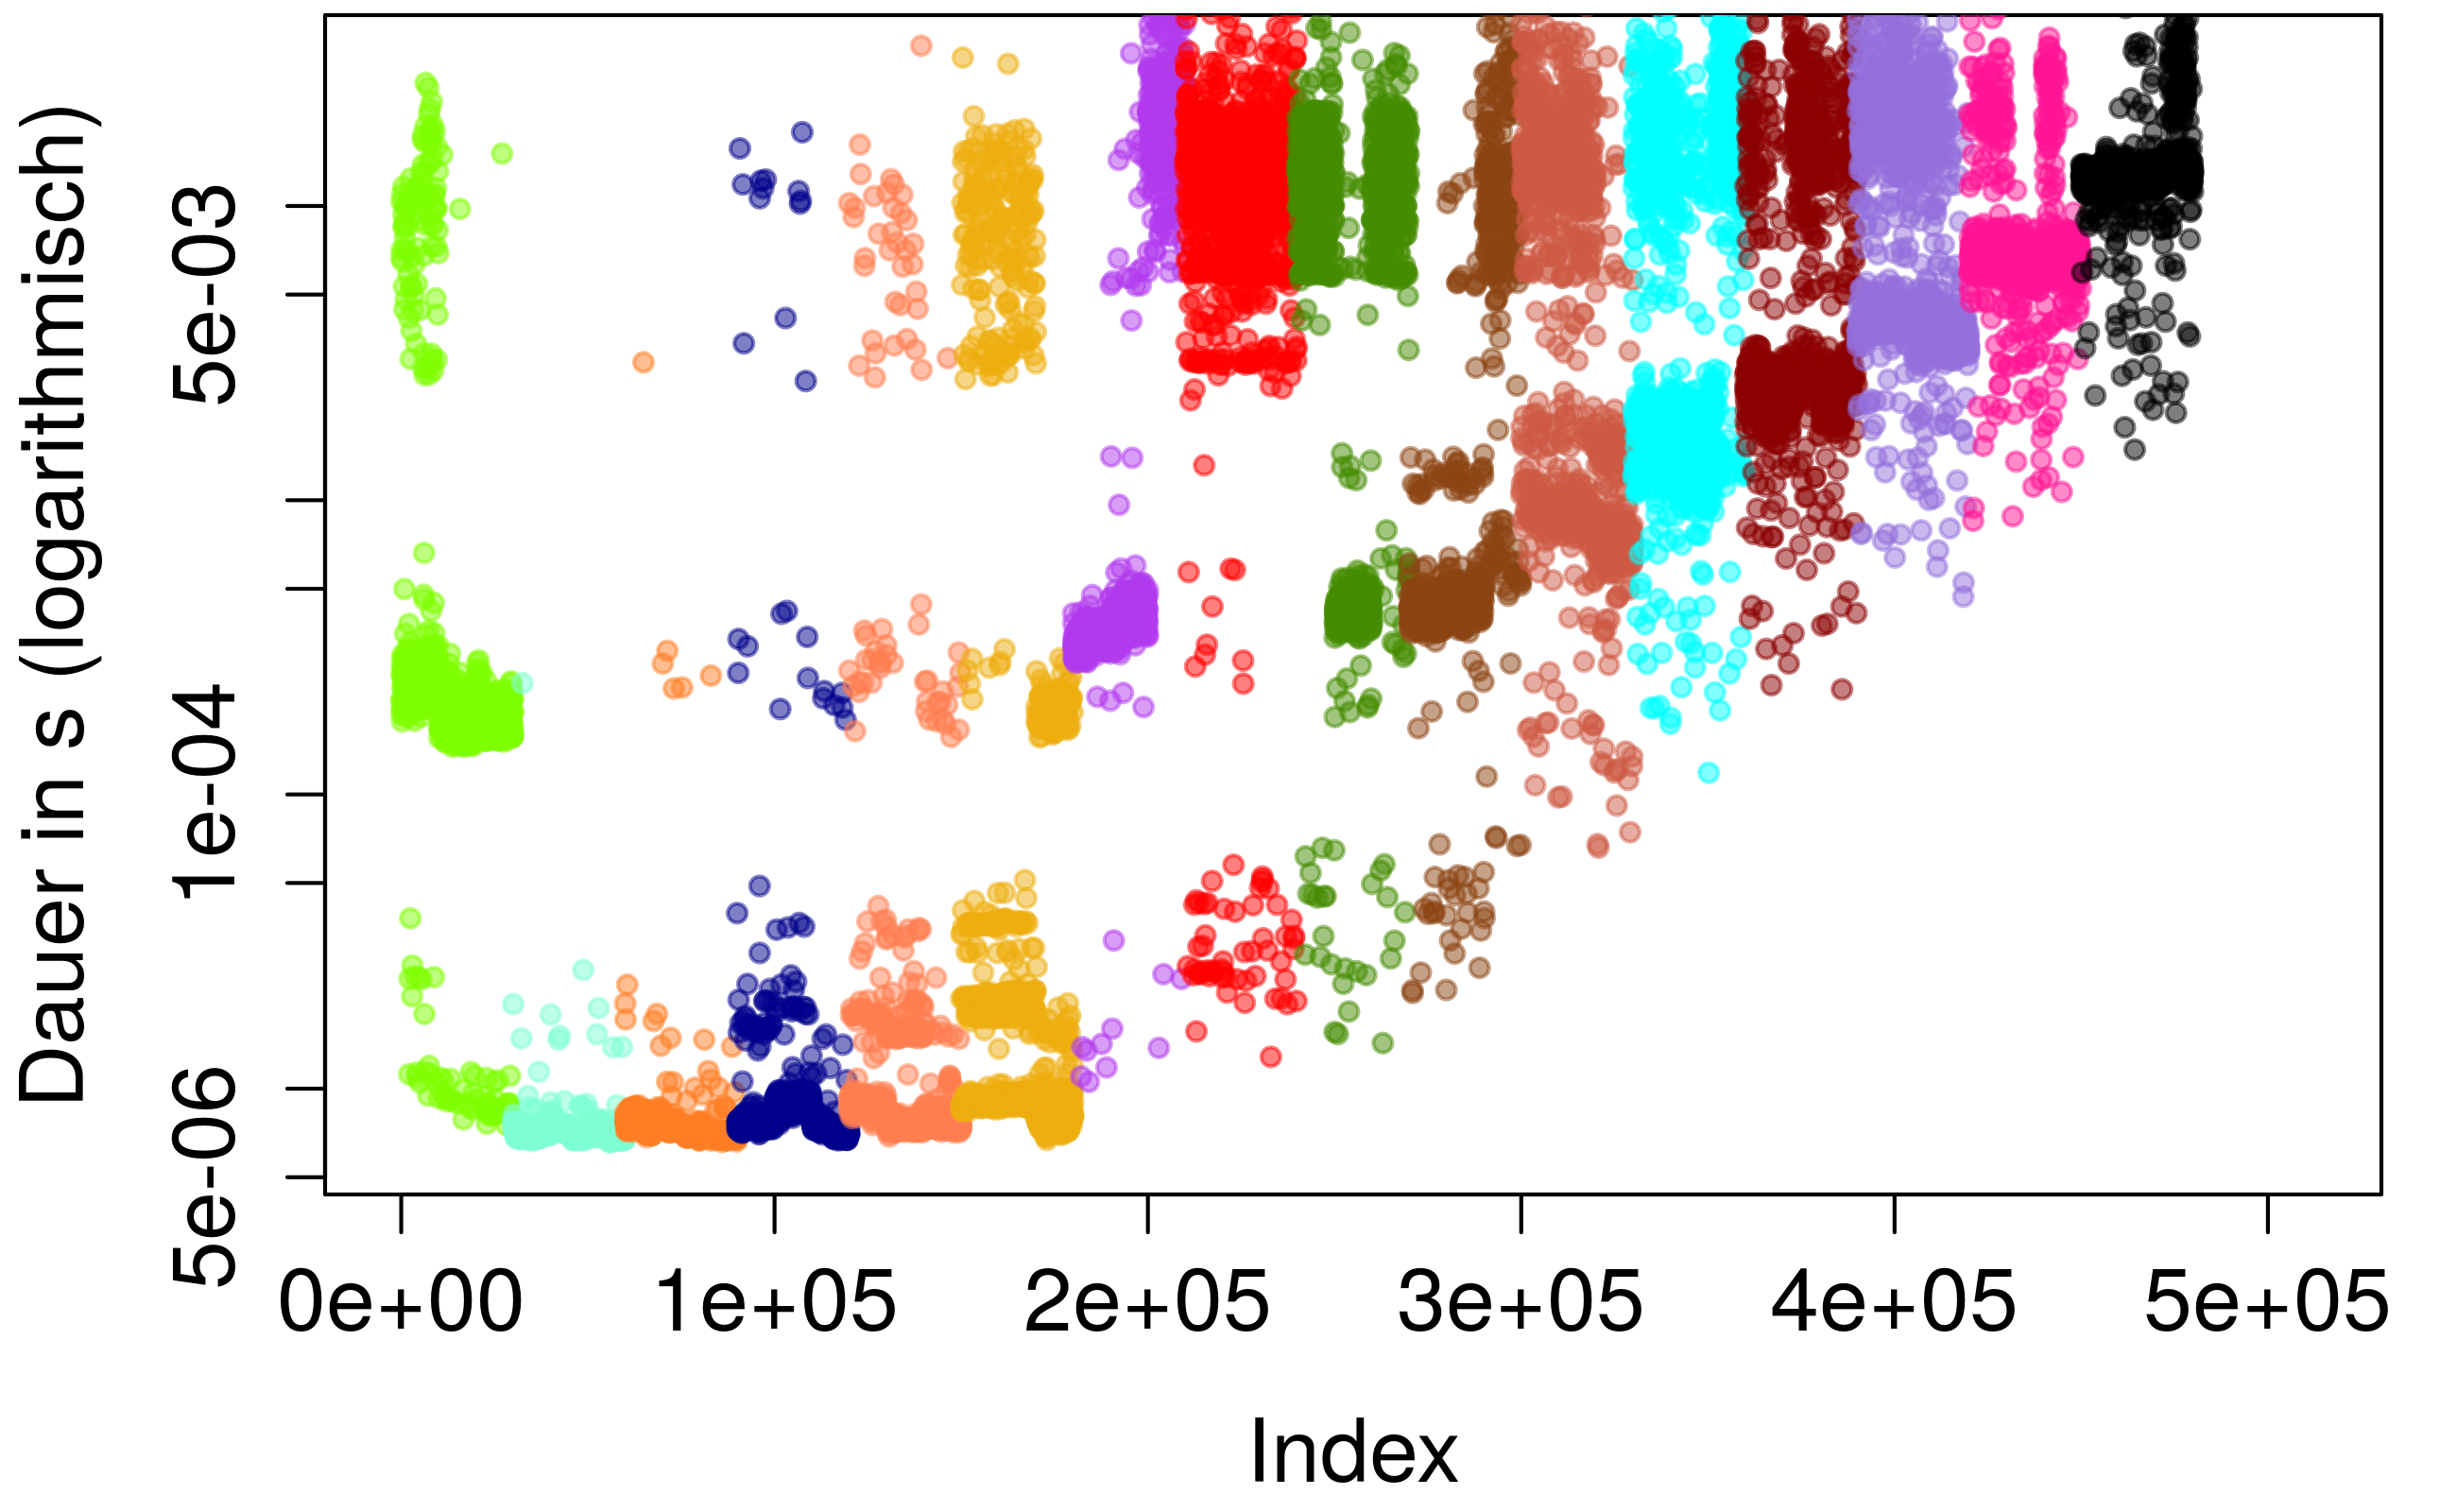
\includegraphics[width=.5\textwidth]{Bilder/Plots/exploration/plot_SizeSorted_log_read_rnd.png}
	}
	\hfill
	\subfloat[Messungen in Zeitreihe zu RND-W]{
		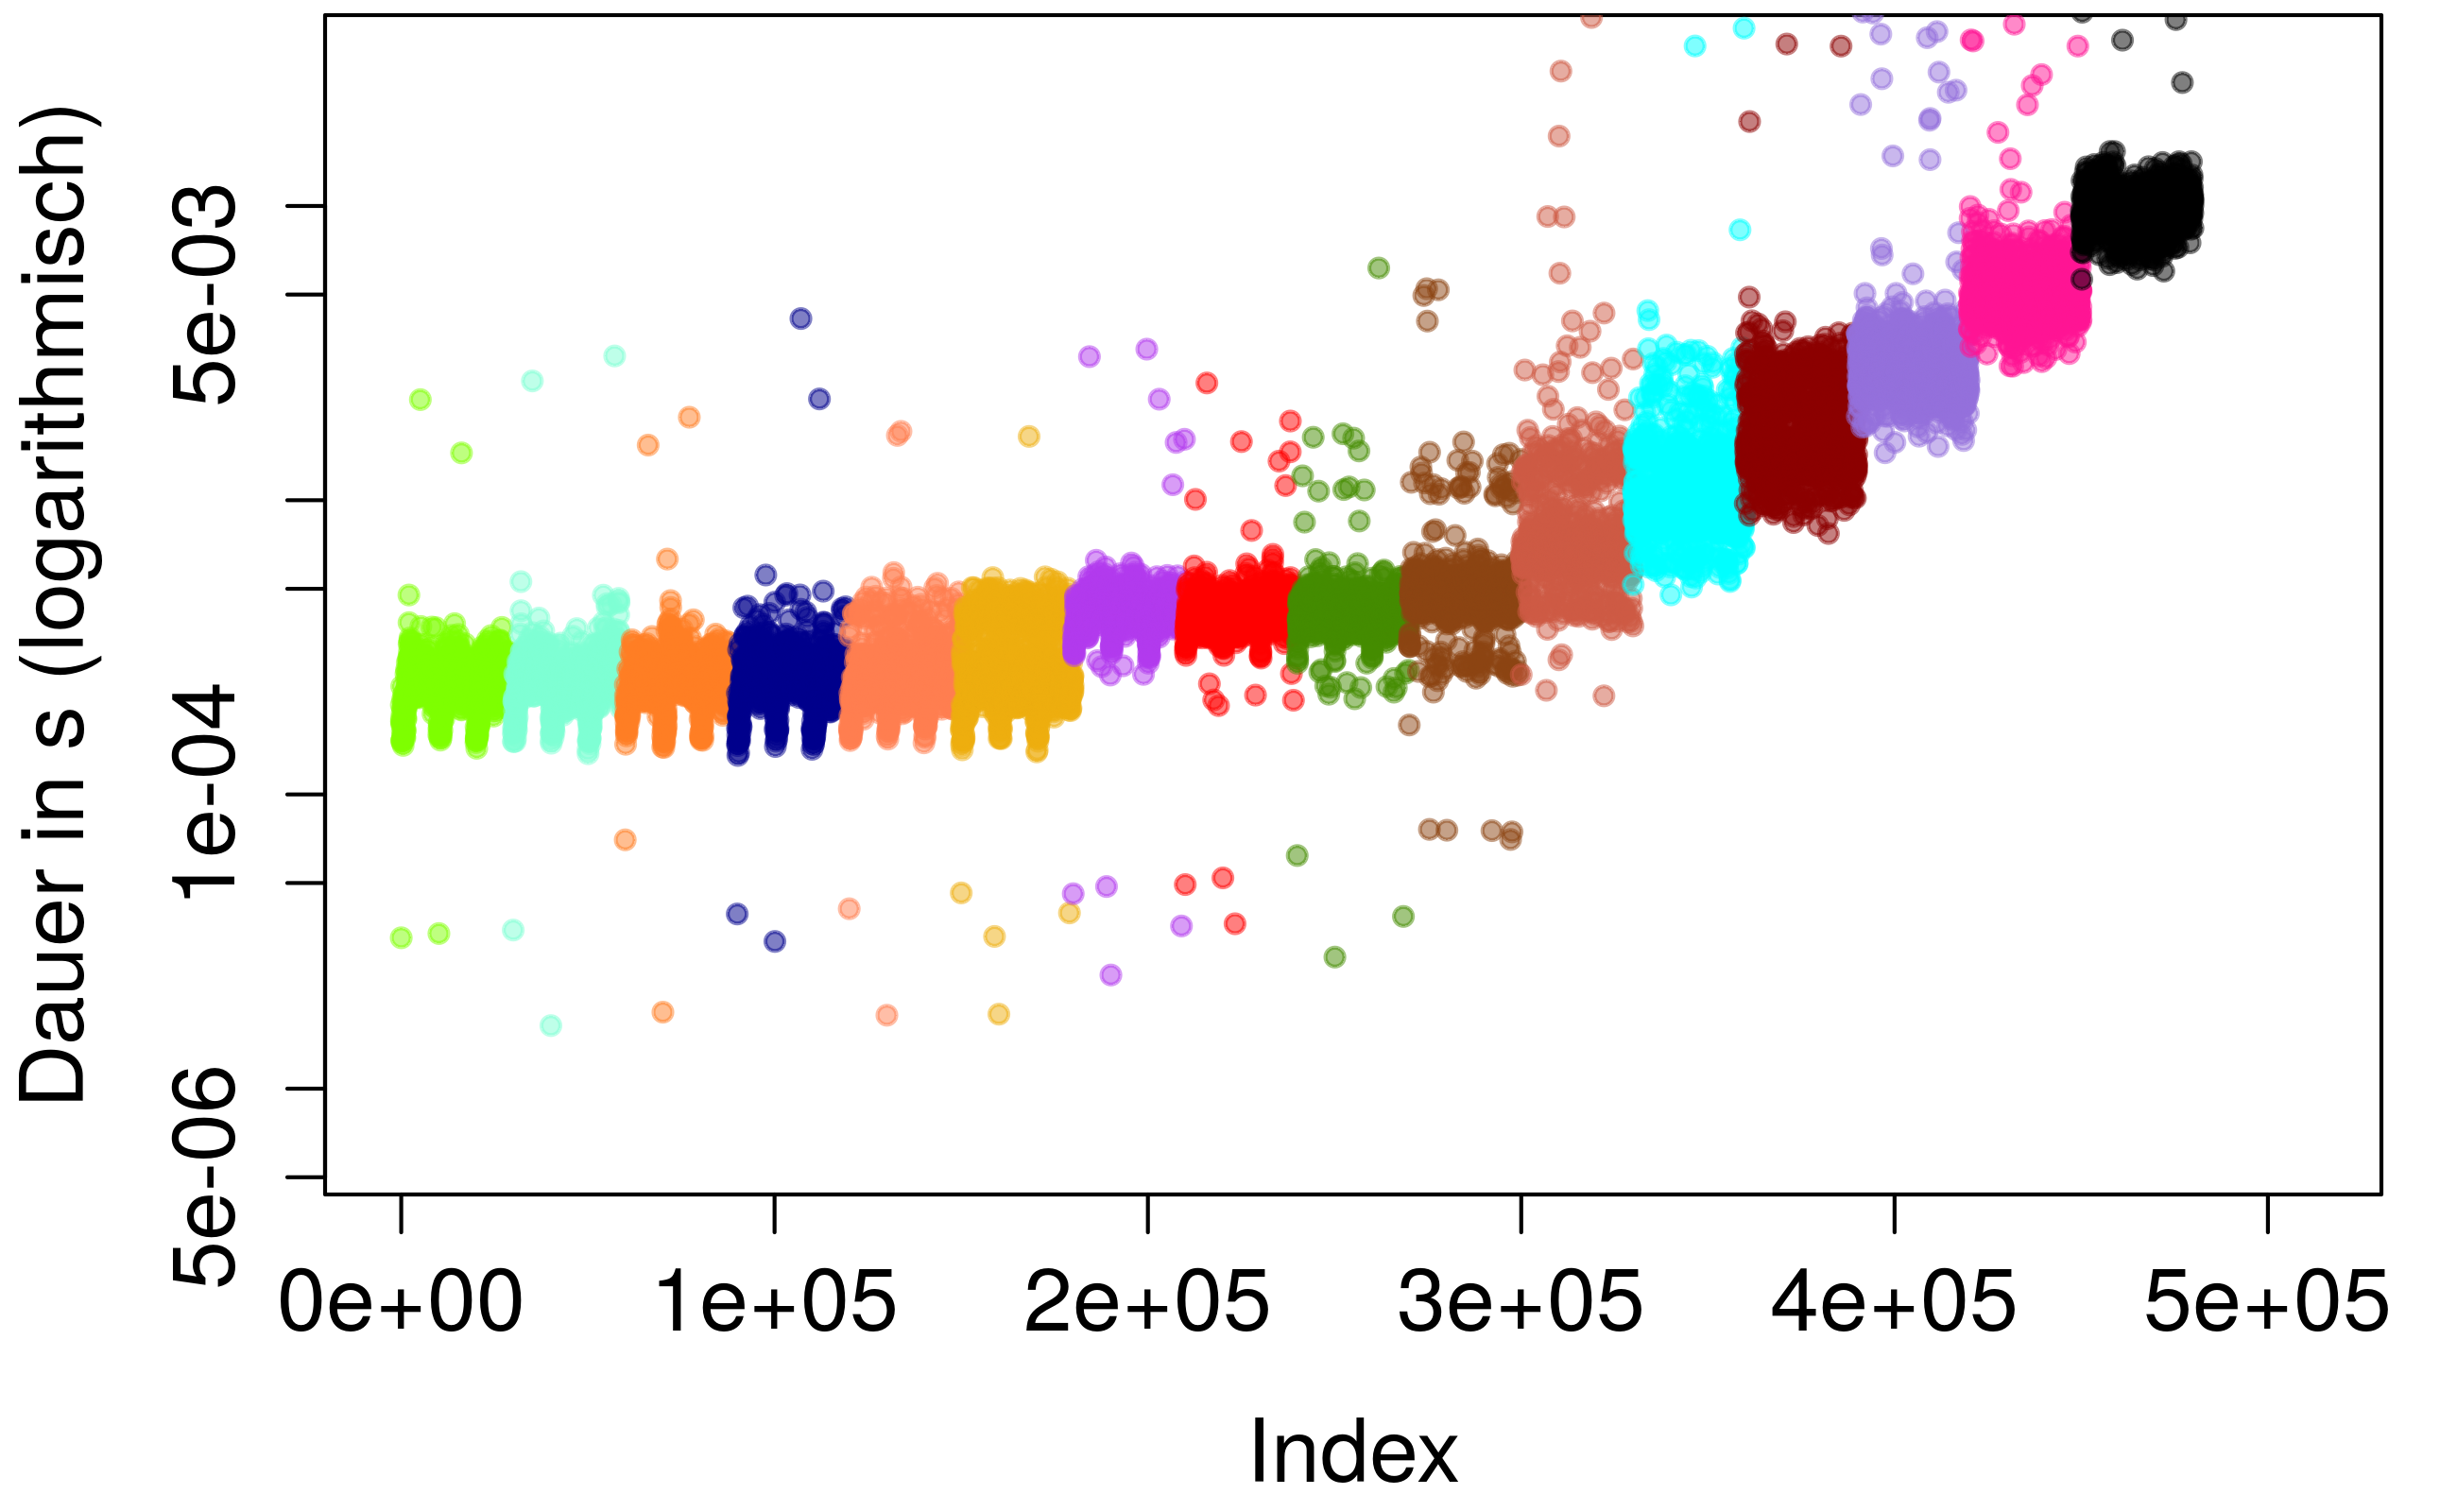
\includegraphics[width=.5\textwidth]{Bilder/Plots/exploration/plot_SizeSorted_log_write_rnd.png}
	}	
	\caption{Messungen der Laufzeiten nach Zugriffsgröße sortiert dargestellt. Von links nach rechts 1B, 4B, 16B, 64B, 256B, 1KiB, 4KiB, 8KiB, 16KiB, 64KiB, 256KiB, 512KiB, 1MiB, 2MiB, 4MiB, 8MiB und 16MiB}
	\label{Laufzeiten_Zeitreihe}
\end{figure} 

\subsubsection{Verteilung der Zugriffszeiten}
Der in Abschnitt \ref{analyse:ea_pfad_zurvorhersage} Beschriebene Zusammenhang zwischen E/A-Pfad und Zugriffszeit wurde anhand von Abbildung \ref{Laufzeiten_Zeitreihe}a verdeutlicht.
Für RND-R ergeben sich ähnliche Beobachtungen, während die Abhängigkeit zwischen E/A-Pfad und Laufzeit bei den beiden Abbildungen zu Messreihen mit zufälligen Dateizugriffen weniger deutlich zu sein scheint. Aber auch hier lässt sich teilweise eine Aufspaltung der Messungen mit gleicher Zugriffsgröße in zwei Gruppen beobachten.\medskip

Wenn die Messpunkte nach der Laufzeit sortiert werden (siehe Abbildung \ref{Laufzeiten_Sortiert}), können die verschiedenen Stufen der Laufzeiten besser betrachtet werden.
Bestimmte Laufzeiten kommen häufiger vor, sie kennzeichnen sich als Auftritt der Stufen. Andere Laufzeiten kommen dagegen seltener vor, sie bilden eine Senkrechte.
Die Stufen entstehen einerseits durch die Messung unterschiedlicher Zugriffsgrößen (mit größeren Abständen zwischen verschiedenen Größen), teilweise lassen sie sich aber auch als die beschriebenen E/A-Pfade im System interpretieren.\medskip

Die geringe Aufteilung der Messungen in Gruppen bei den beiden Datensätzen zu schreibenden E/A-Aufrufen, sprechen dafür, dass die Stufen der Messung verschiedener Zugriffsgrößen zuzusprechen ist.
Der andere Fall lässt sich besonders gut bei RND-R erkennen. Die Zugriffszeiten zu einer Größe teilen sich in Abbildung \ref{Laufzeiten_Zeitreihe}c in etwa drei Gruppen auf, eine langsame, eine mittlere und eine schnelle.
Die Gruppen verschiedener Zugriffsgrößen können teilweise zu einem E/A-Pfad zusammengefasst werden. Die Häufungen finden sich dann auf einer horizontalen Linie. 
Die Laufzeit ist für die horizontal nebeneinanderliegenden Gruppen nicht vorwiegend von der Zugriffsgröße abhängig, sondern in unserer Interpretation von dem Pfad, den die entsprechenden Aufrufe im System genommen haben. 

\begin{figure}
	\subfloat[Messungen sortiert nach Laufzeit für SEQ-R]{
		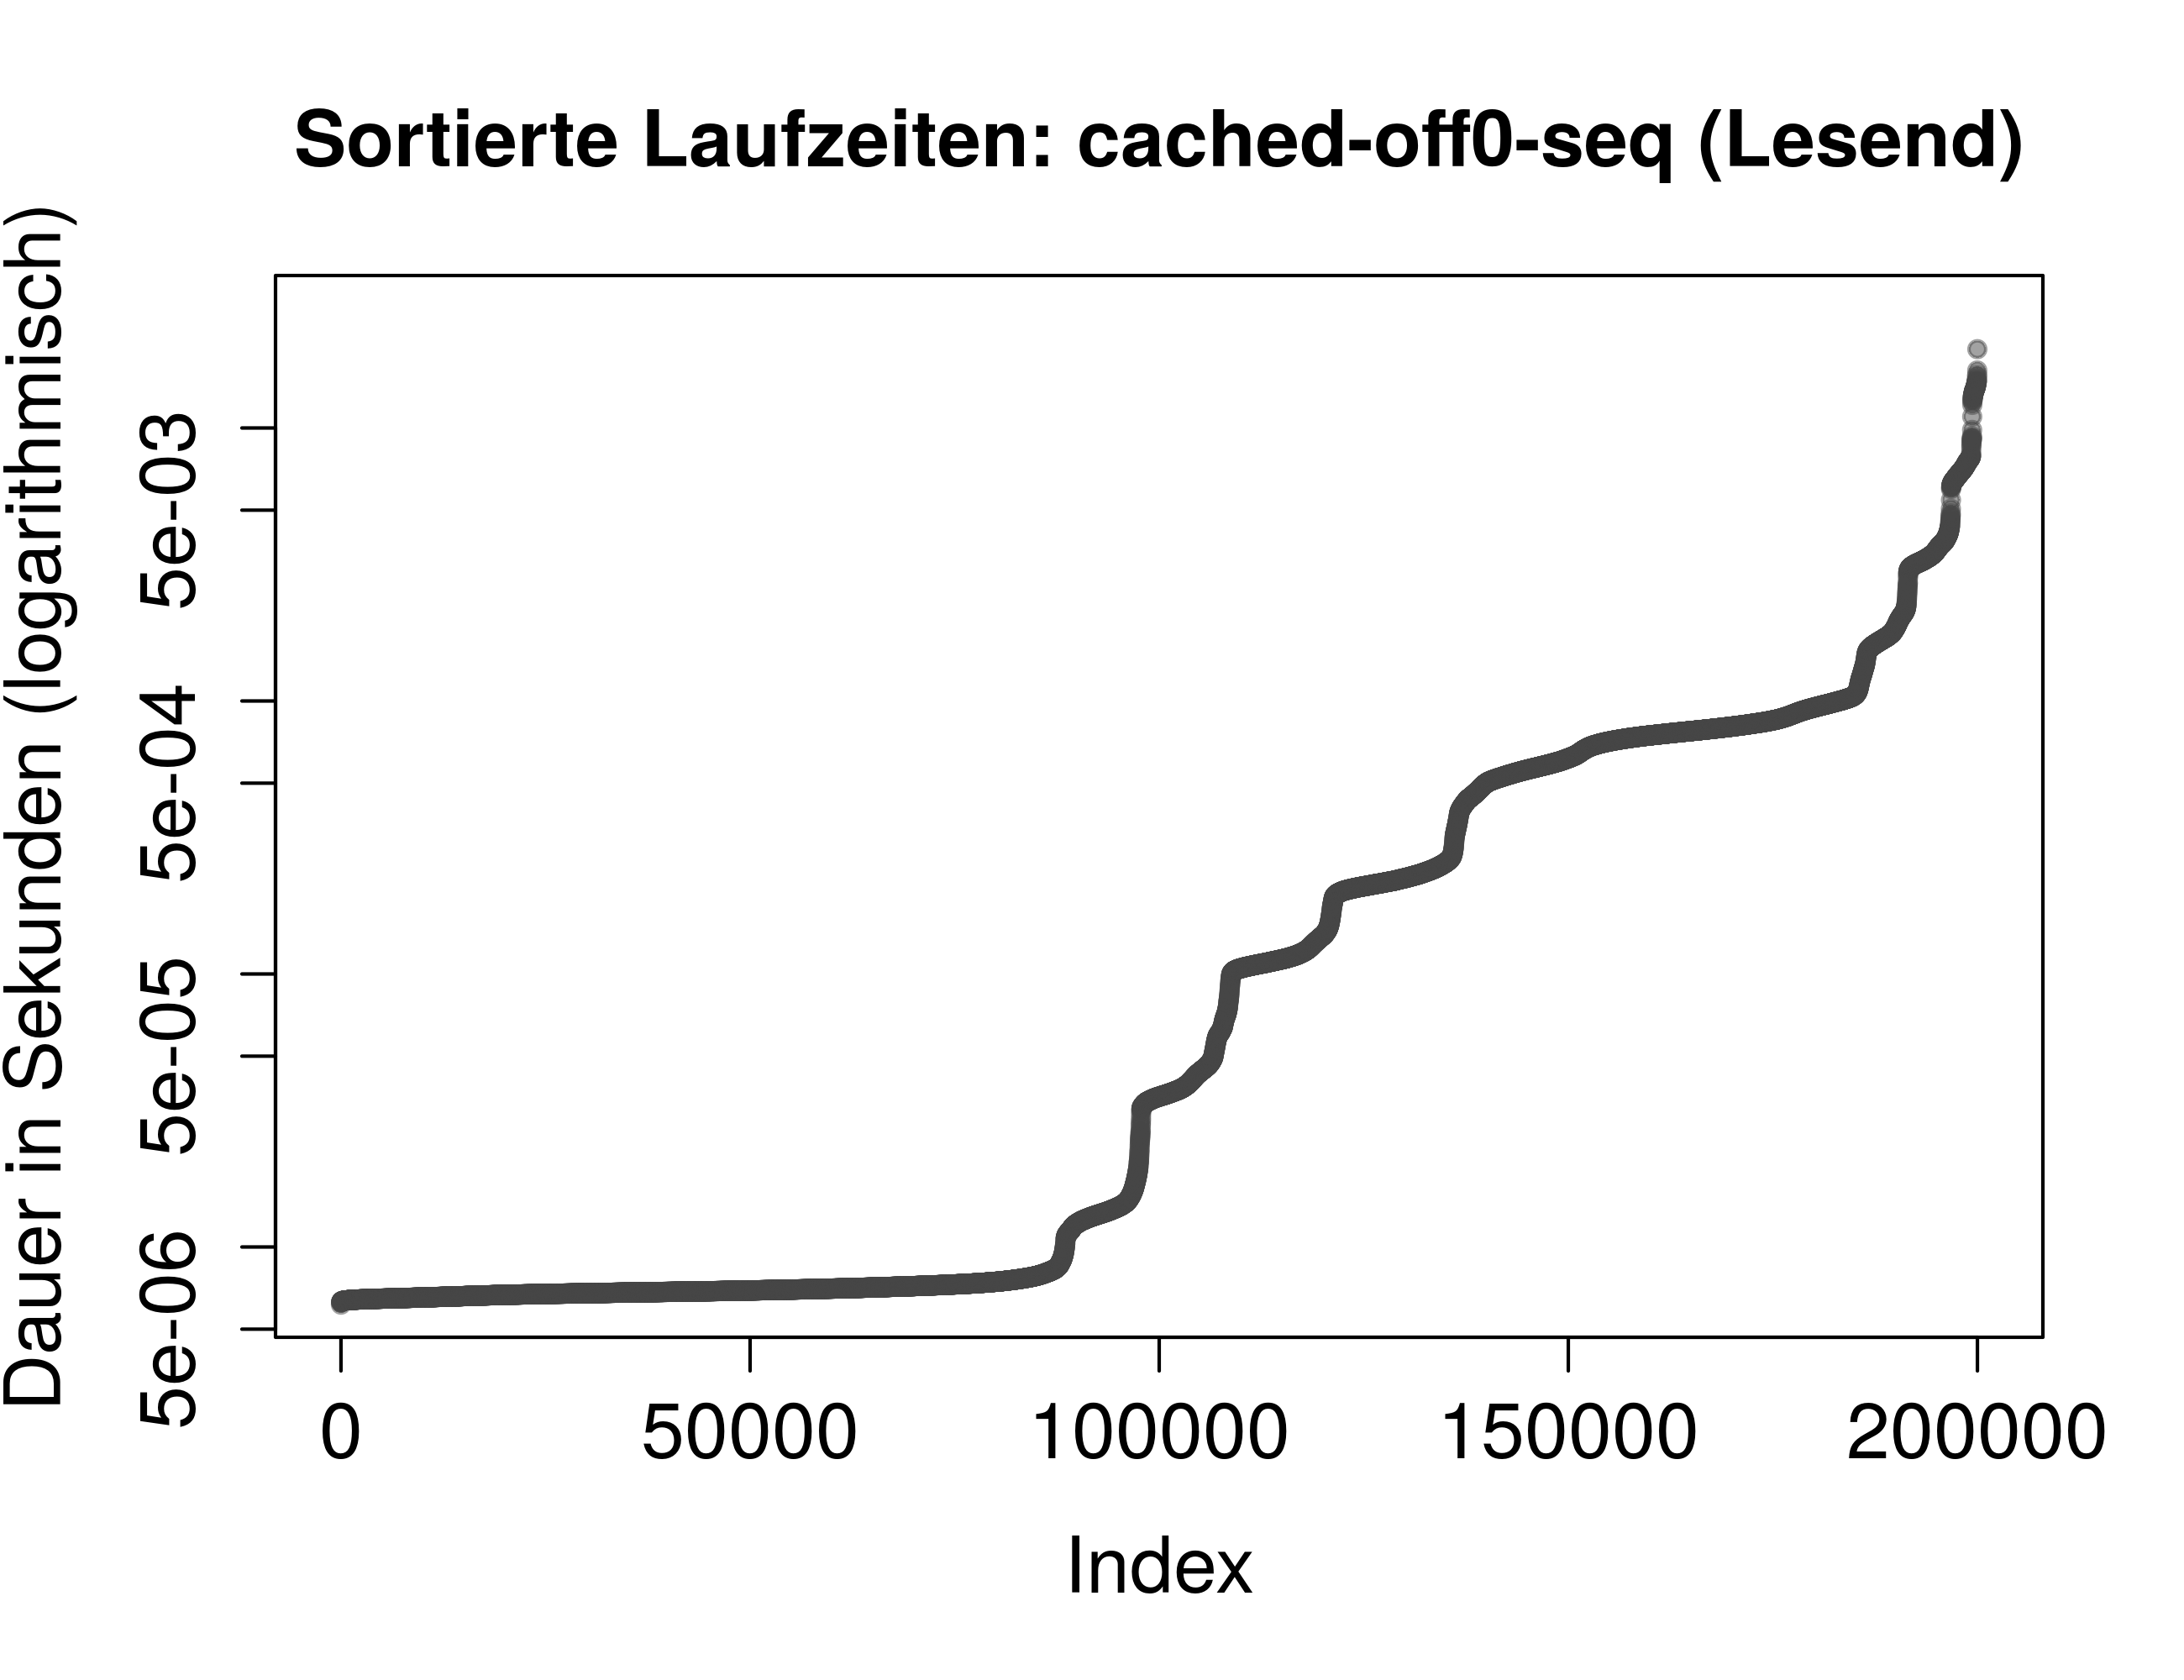
\includegraphics[width=.43\textwidth]{Bilder/Plots/exploration/plot_DurationSorted_read_seq.png}
	}
	\hfill
	\subfloat[Messungen sortiert nach Laufzeit für SEQ-W]{
		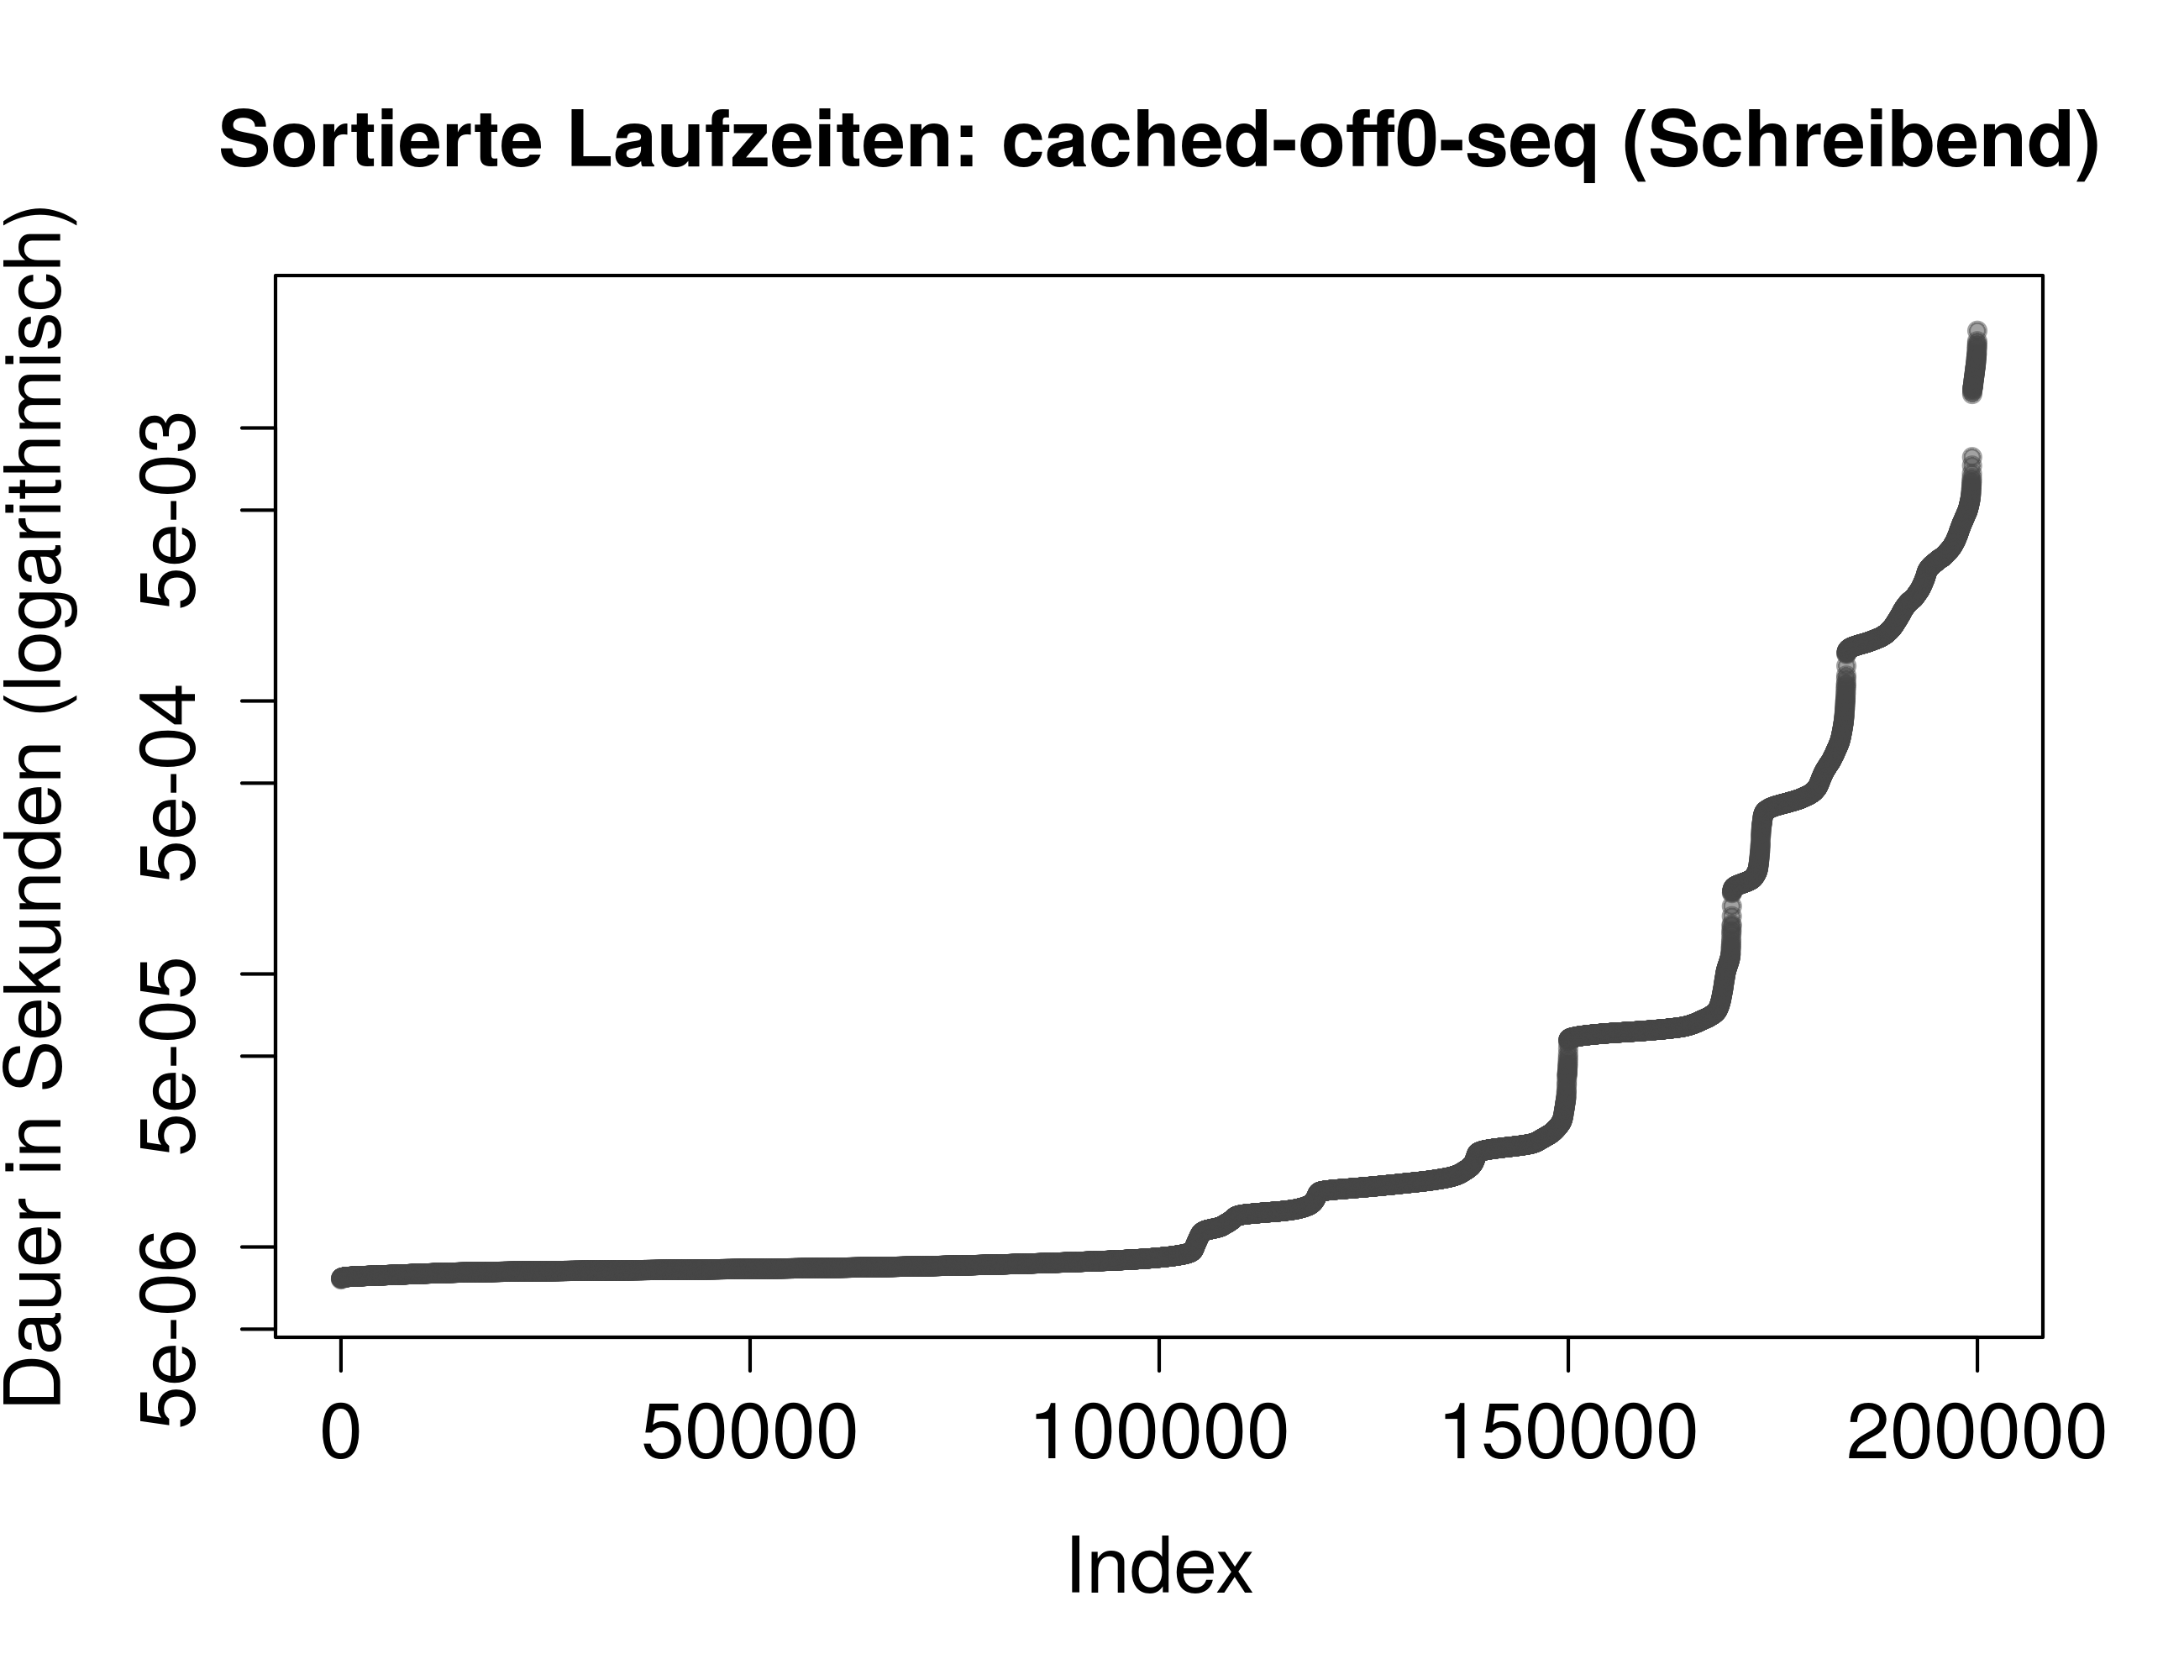
\includegraphics[width=.43\textwidth]{Bilder/Plots/exploration/plot_DurationSorted_write_seq.png}
	}\\
	\subfloat[Messungen sortiert nach Laufzeit für RND-R]{
		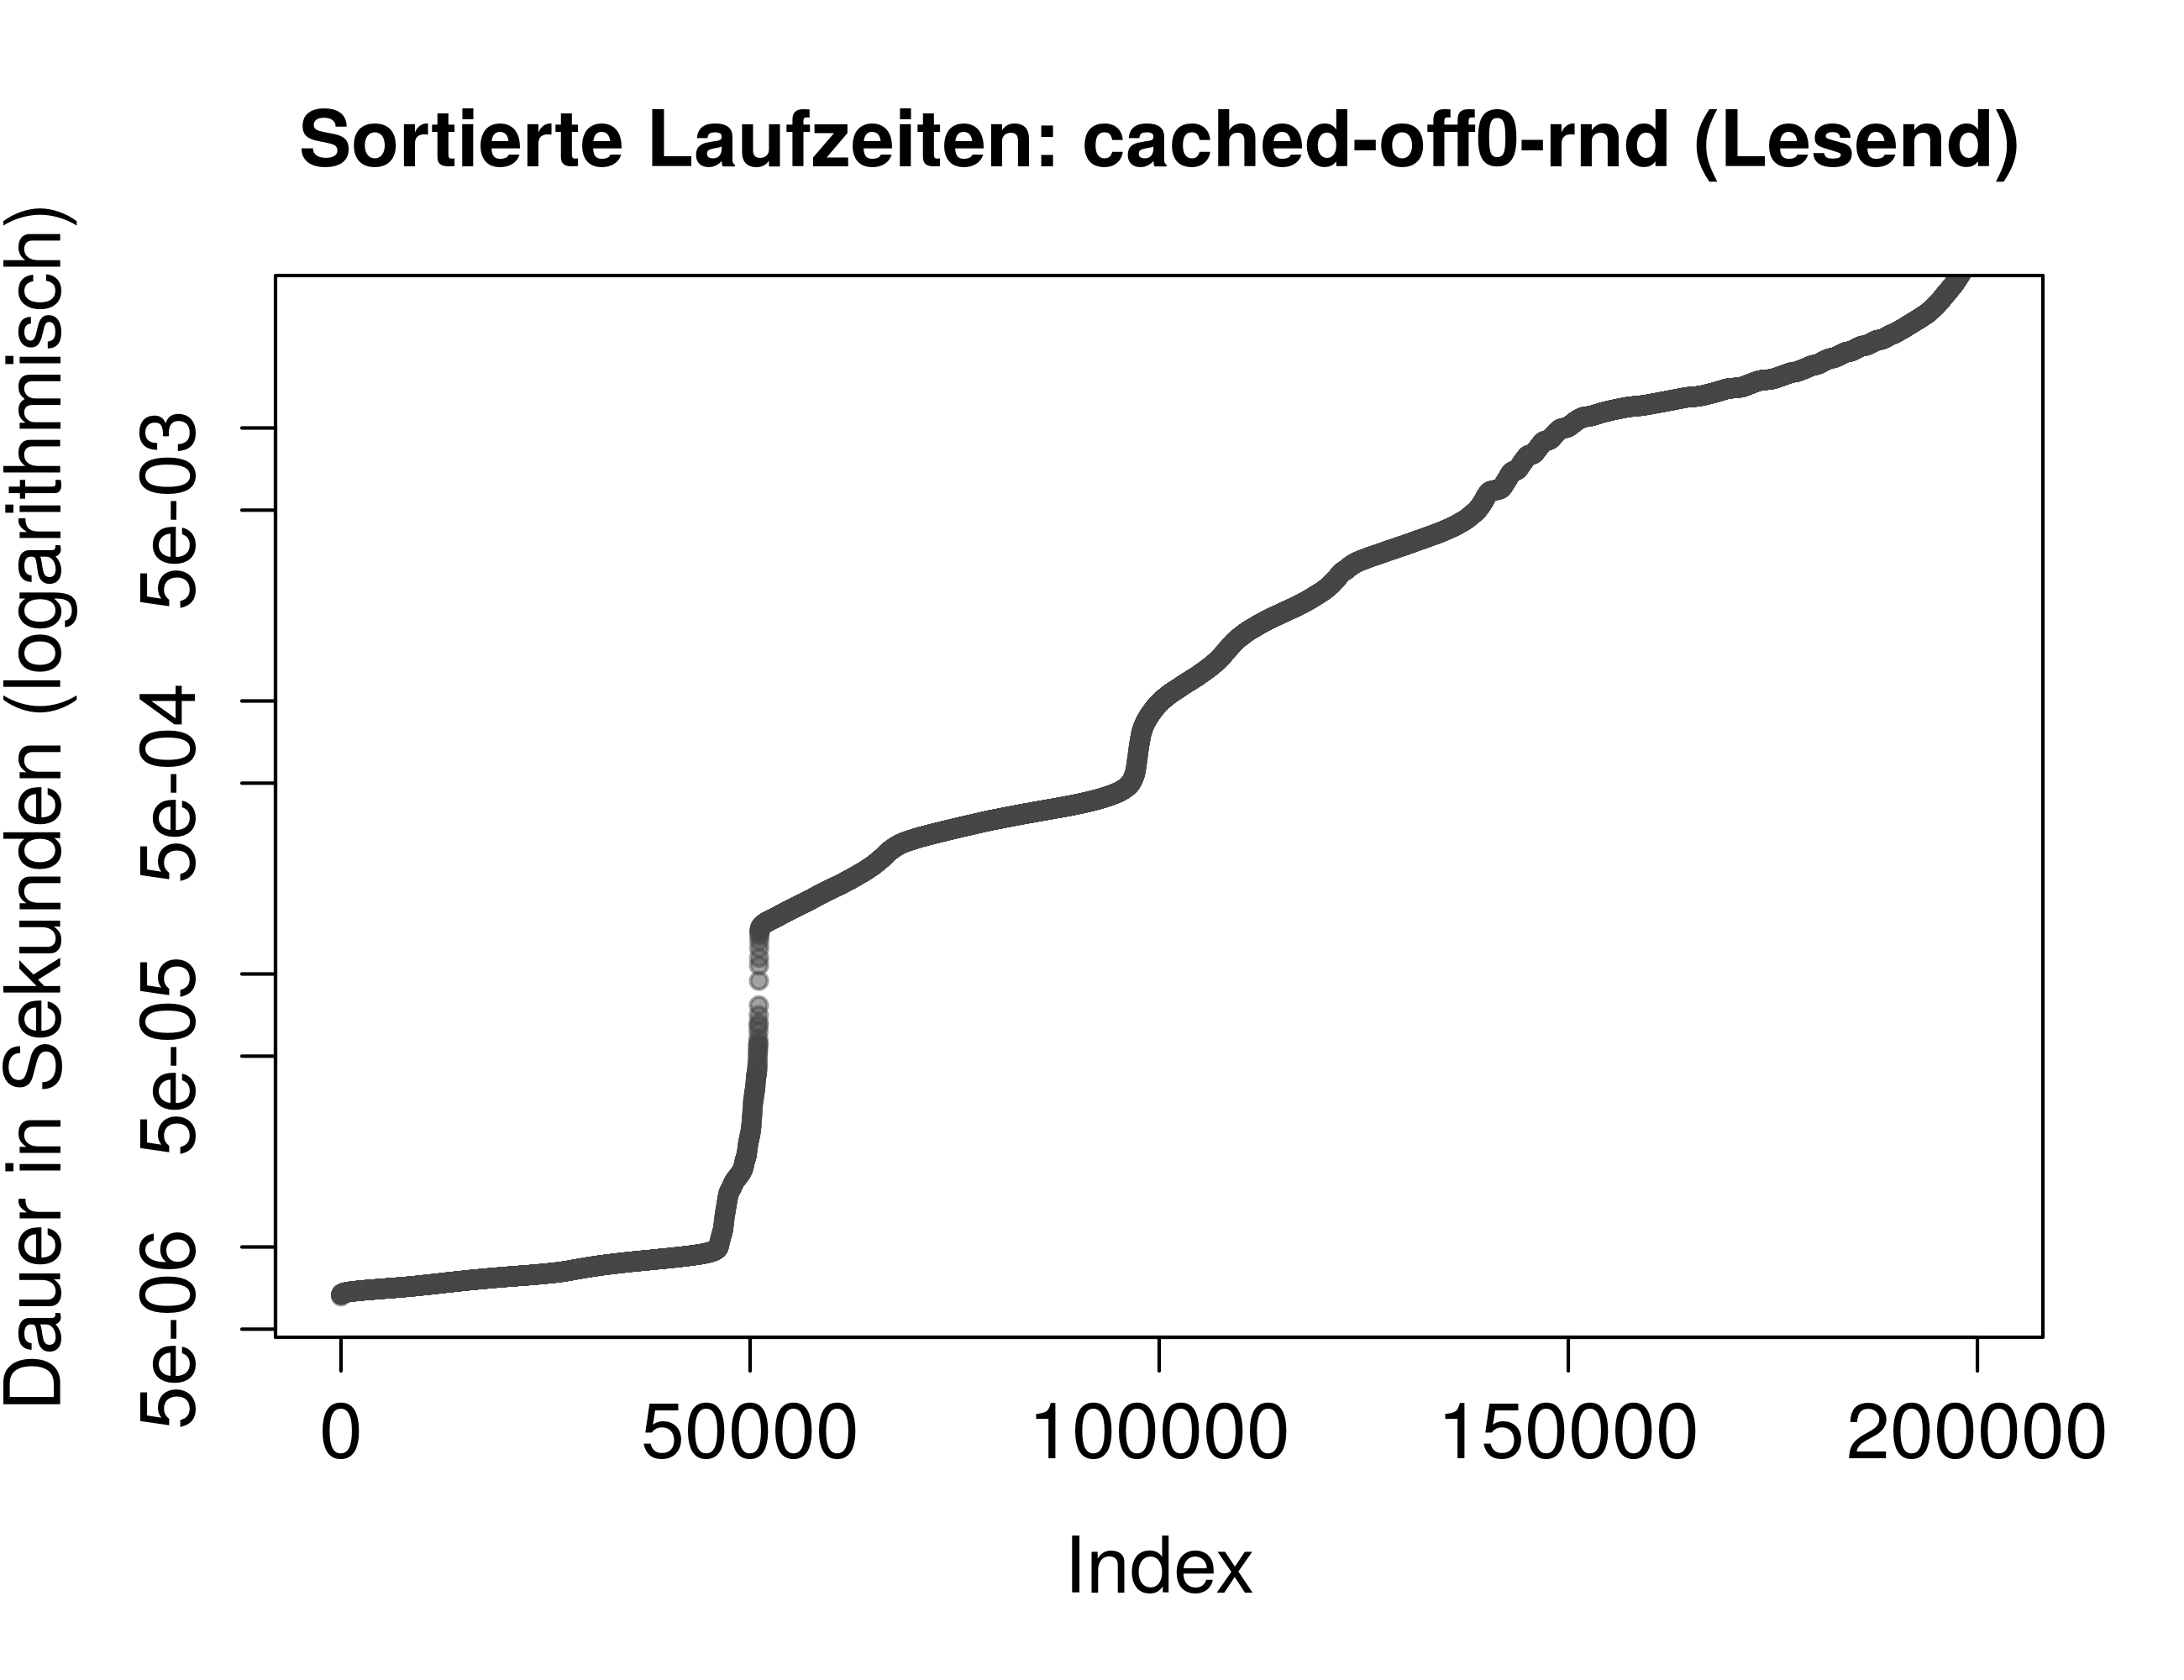
\includegraphics[width=.43\textwidth]{Bilder/Plots/exploration/plot_DurationSorted_read_rnd.png}
	}
	\hfill
	\subfloat[Messungen sortiert nach Laufzeit für RND-W]{
		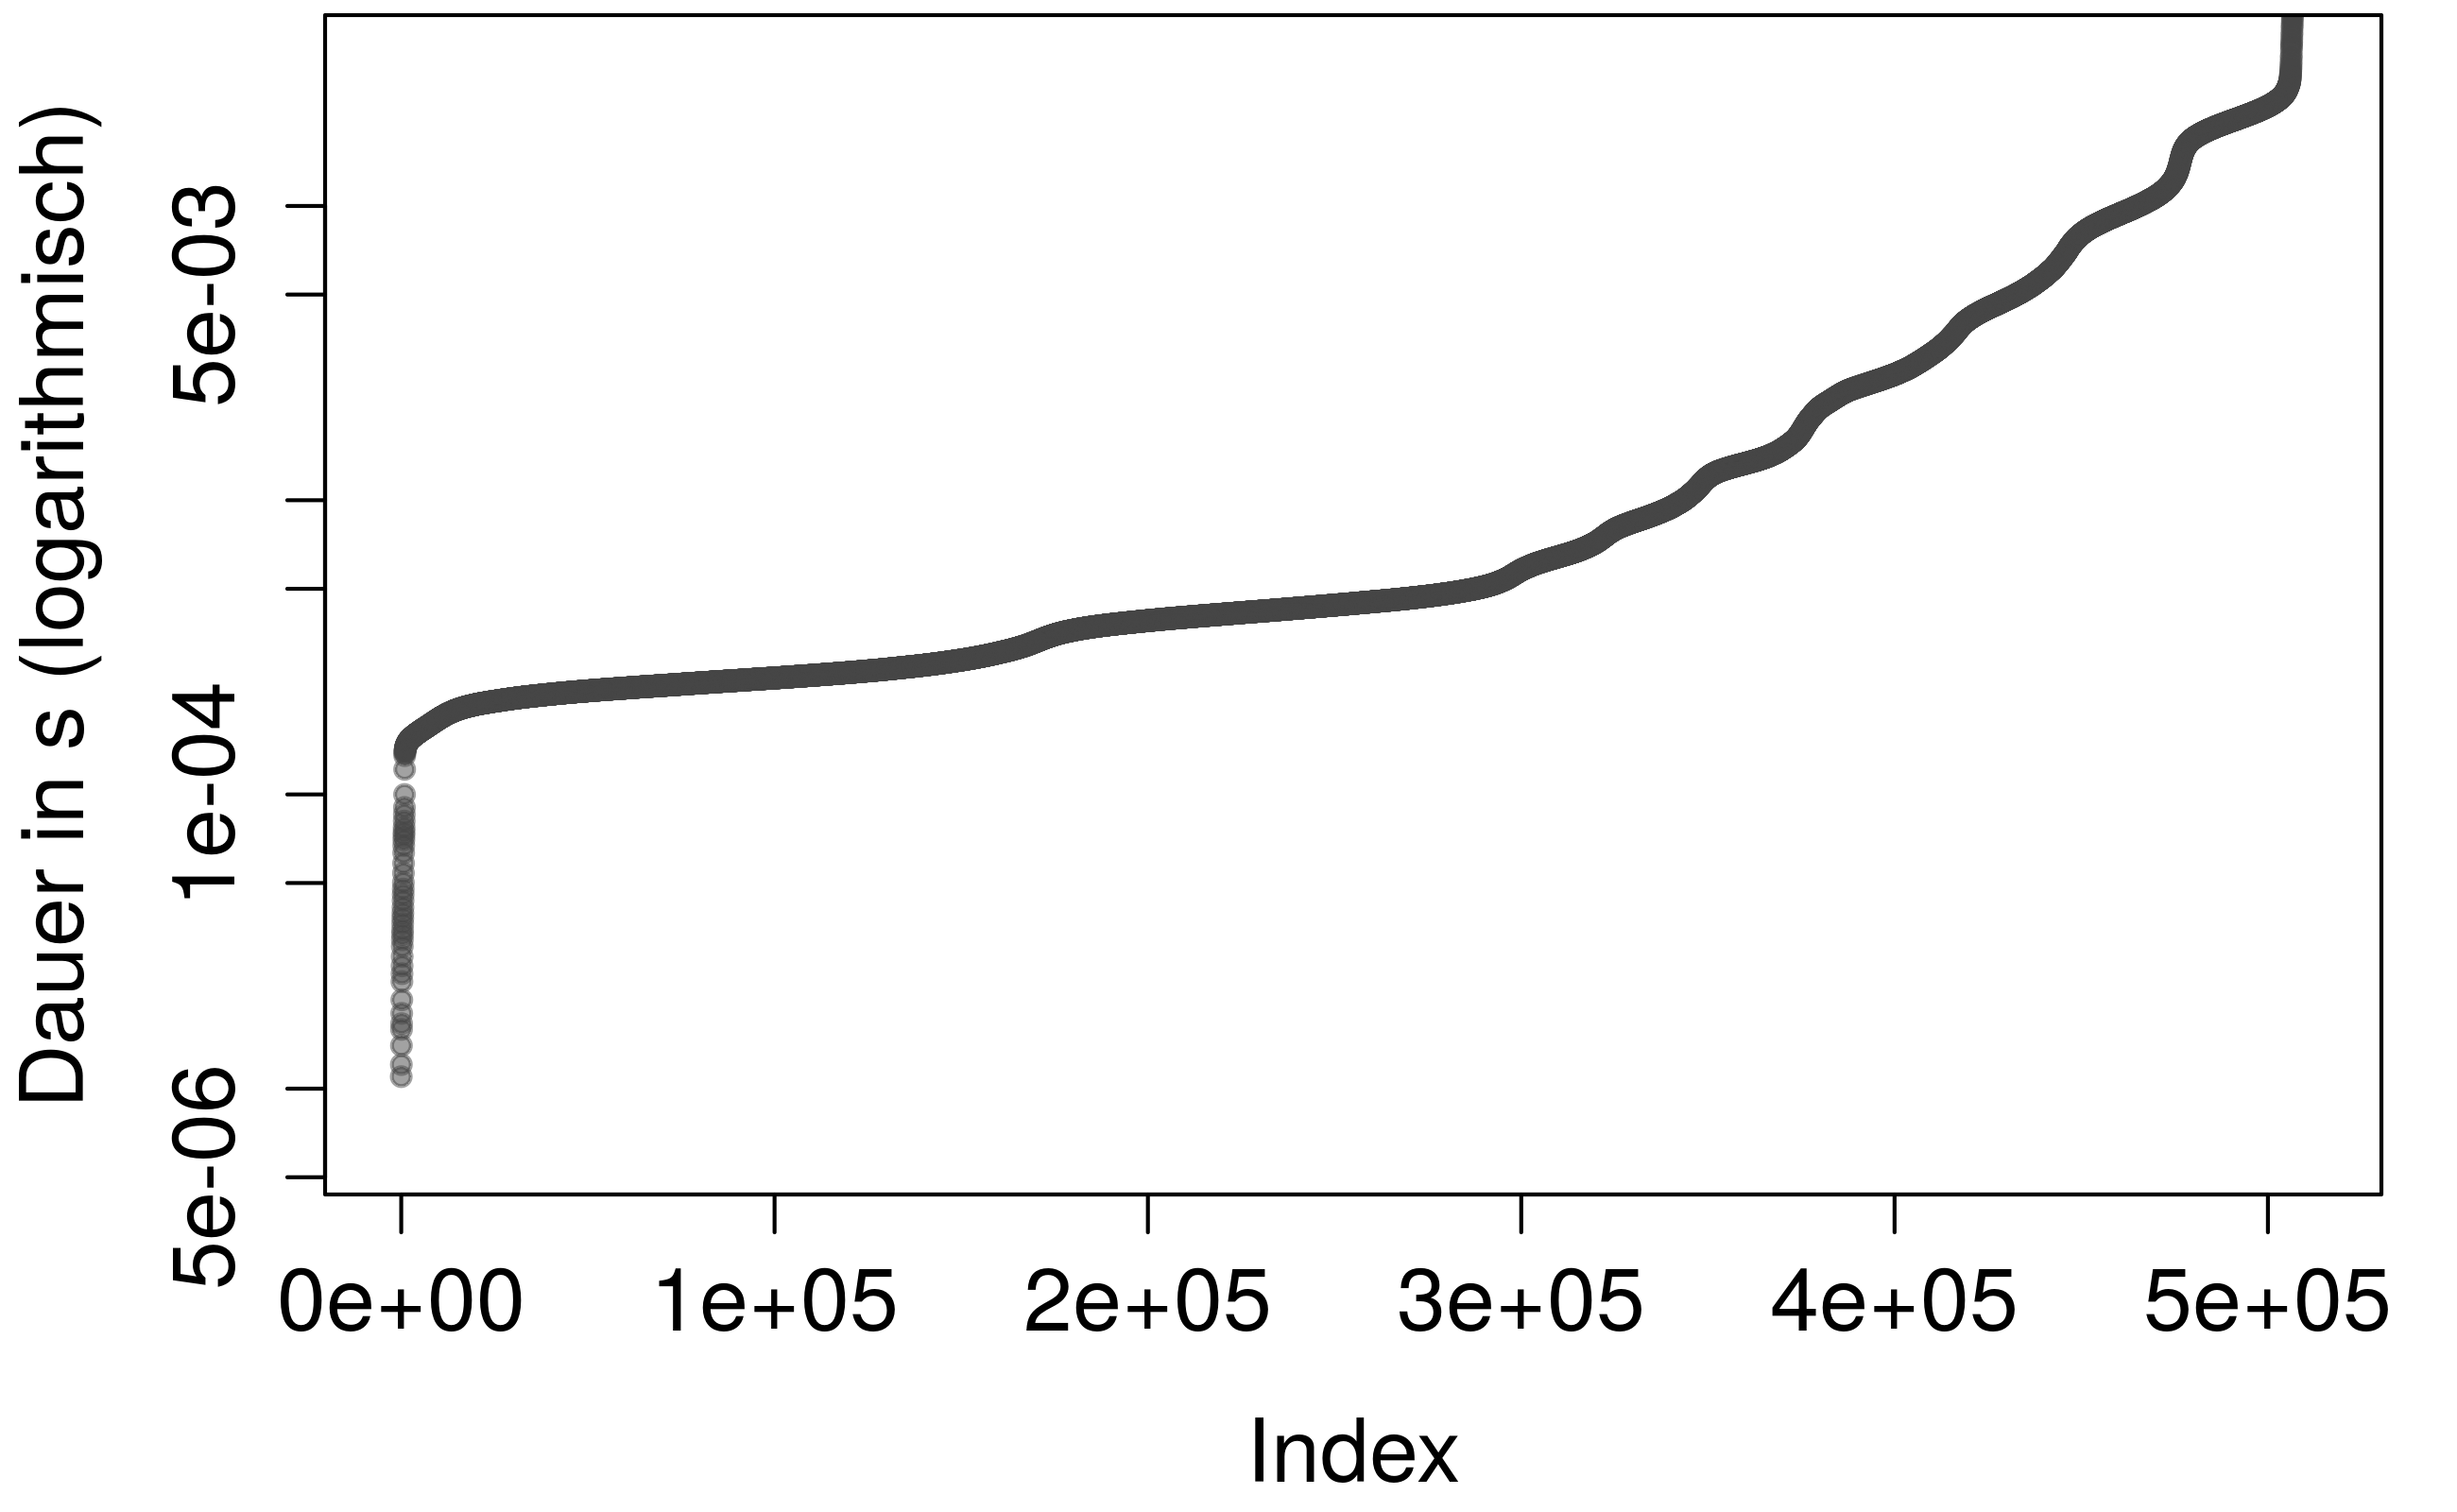
\includegraphics[width=.43\textwidth]{Bilder/Plots/exploration/plot_DurationSorted_write_rnd.png}
	}		
	\caption{Messungen der Laufzeiten sortiert dargestellt.}
	\label{Laufzeiten_Sortiert}
\end{figure} 

\subsubsection{Betrachtung der Ausreißer}
Als Ausreißer werden für alle Attribut-Tupel die Messungen mit den $10\%$ kürzesten und längsten Laufzeiten behandelt. Die Verteilung der Ausreißer ist in Abbildung \ref{fig:ausreisser} zu erkennen.
Bei den randomisierten Messungen gibt es pro Attribut-Tupel nur ein bis drei Messungen. Eine Ausreißerbetrachtung, wie sie hier gemacht wird, macht auf den entsprechenden Datensätzen keinen Sinn. Die Stichprobe zu den verschiedenen Attribut-Tupel ist dafür zu klein.
Die Ausreißervorhersage wird dementsprechend im Folgenden nur auf dem sequentiellen Datensatz durchgeführt.
In Abbildung \ref{fig:ausreisser} sind die Ausreißer rot markiert, sie befinden sich gerade an den oberen und unteren Enden einer Stufe.

\begin{figure}
	\subfloat[Ausreißer auf SEQ-R]{
		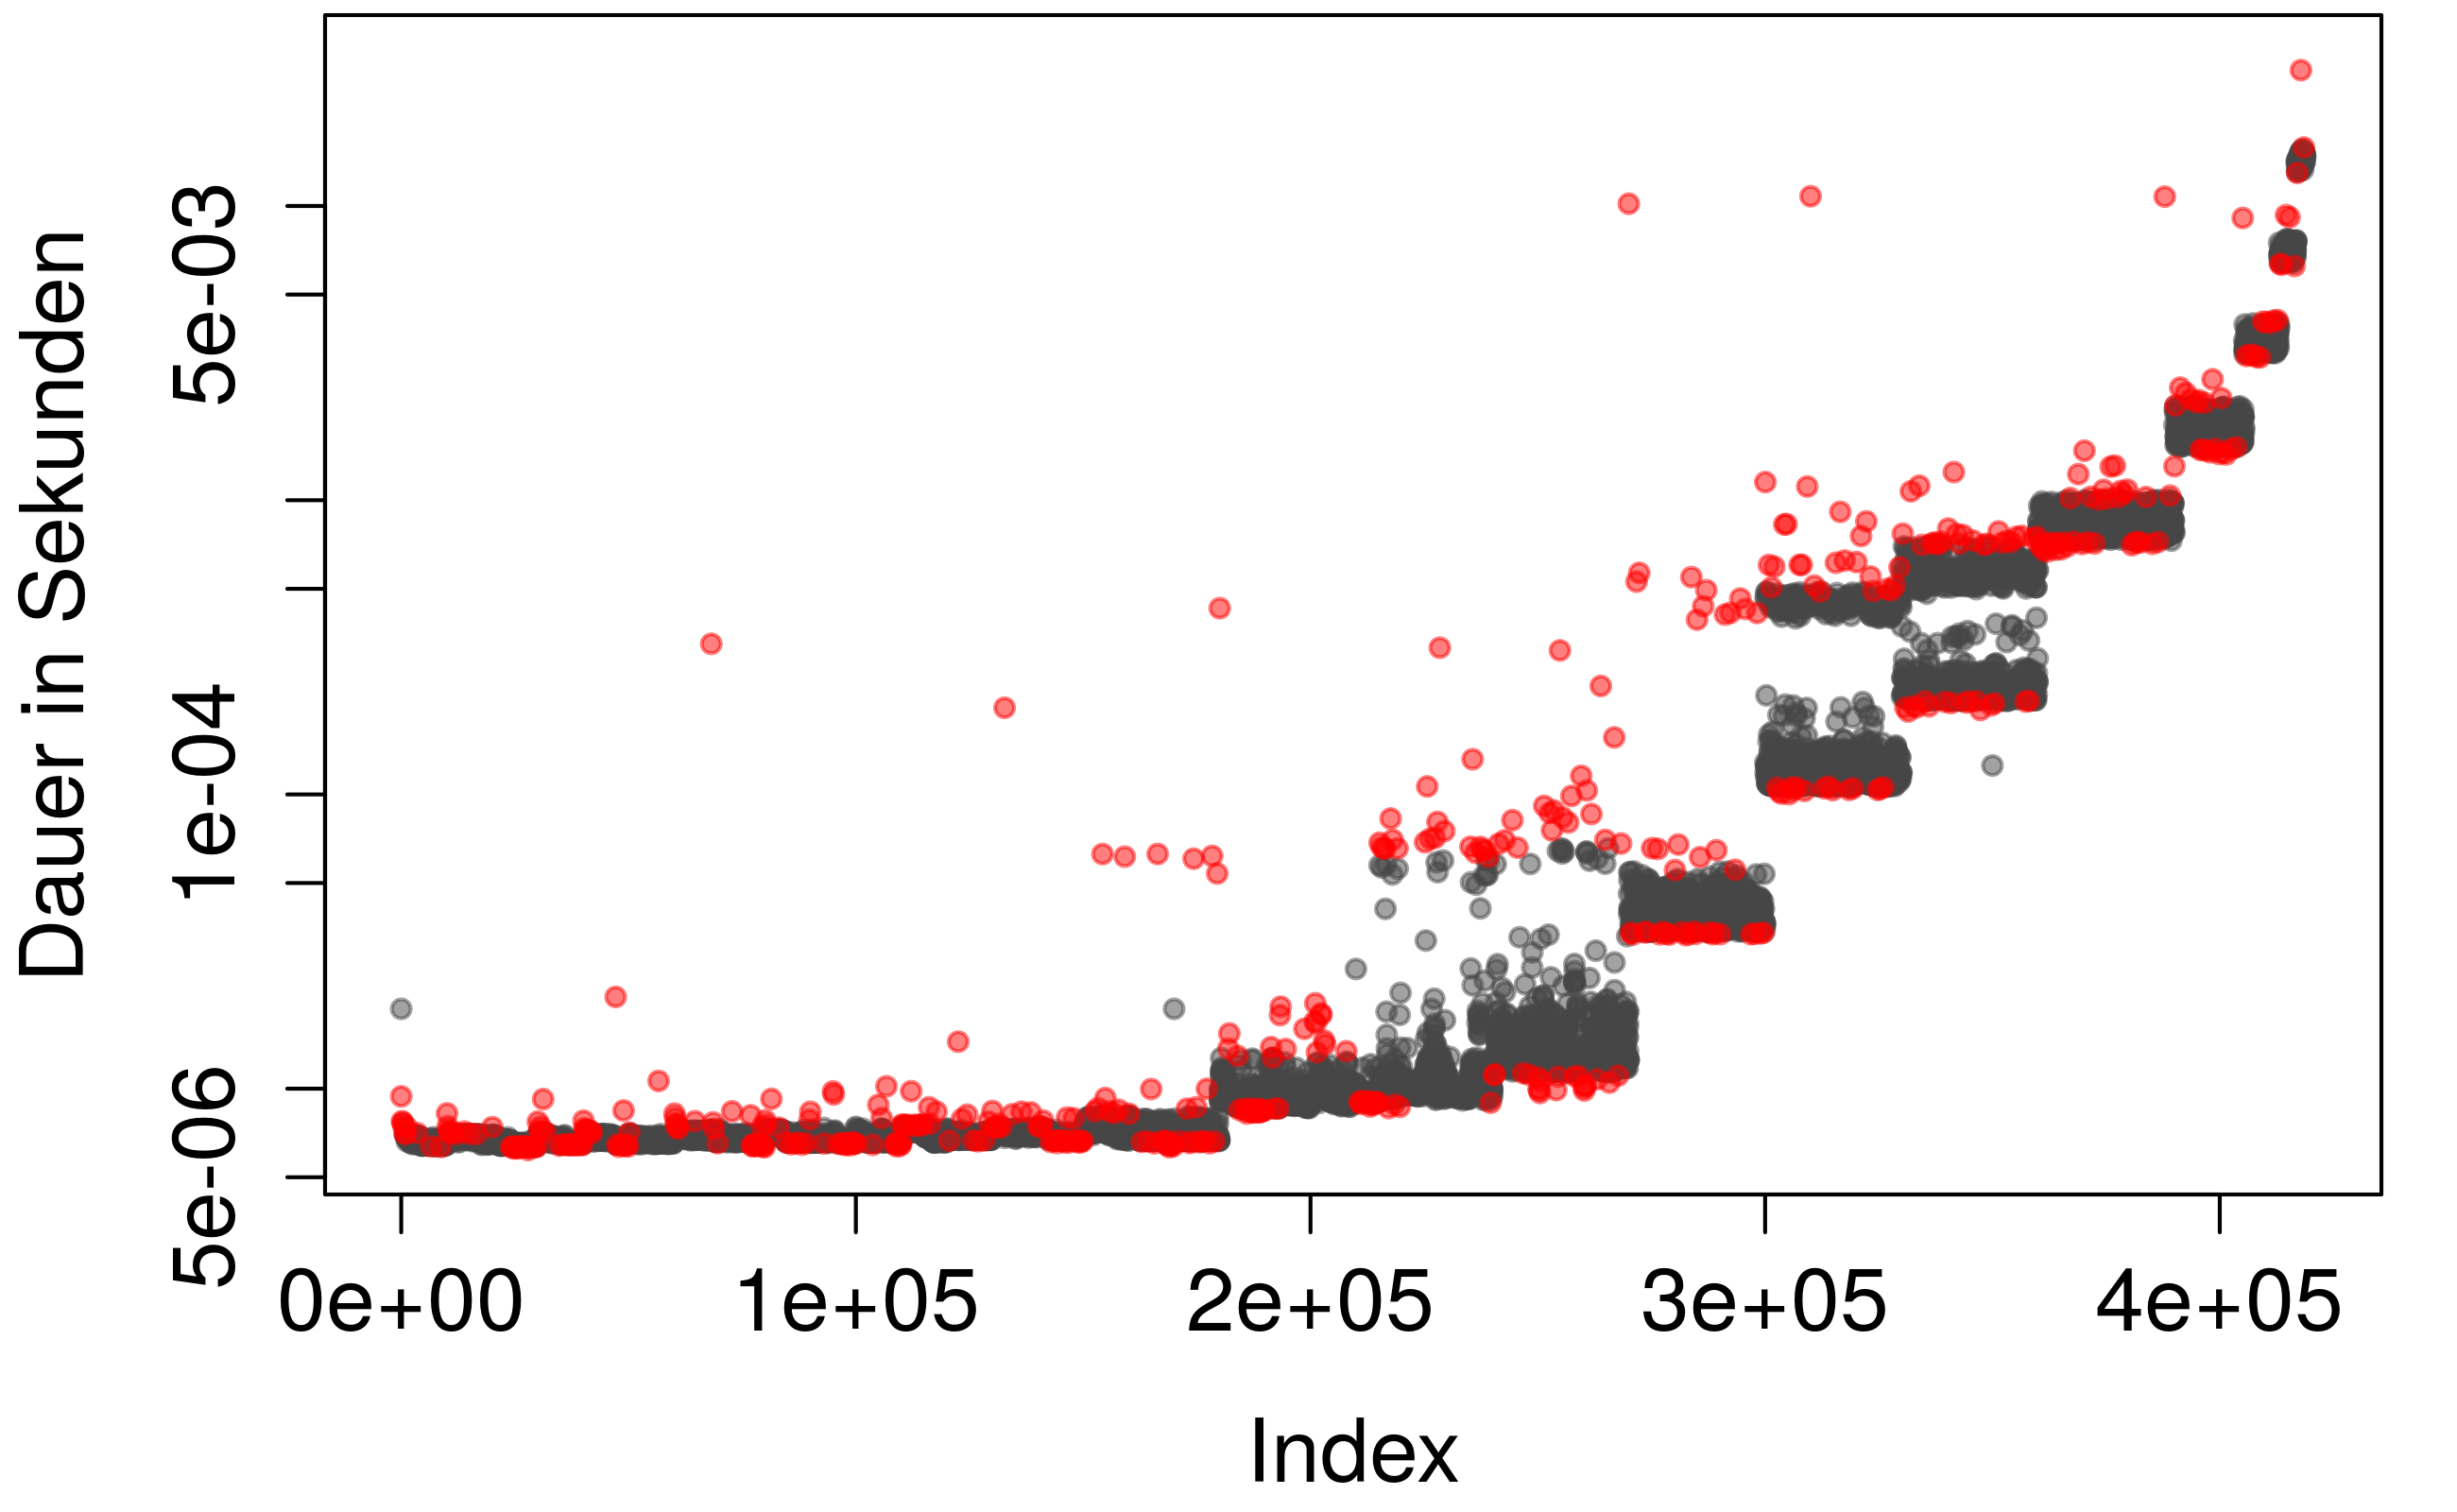
\includegraphics[width=.43\textwidth]{Bilder/Plots/exploration/plot_outlier_read_seq.png}
	}
	\hfill
	\subfloat[Ausreißer auf SEQ-W]{
		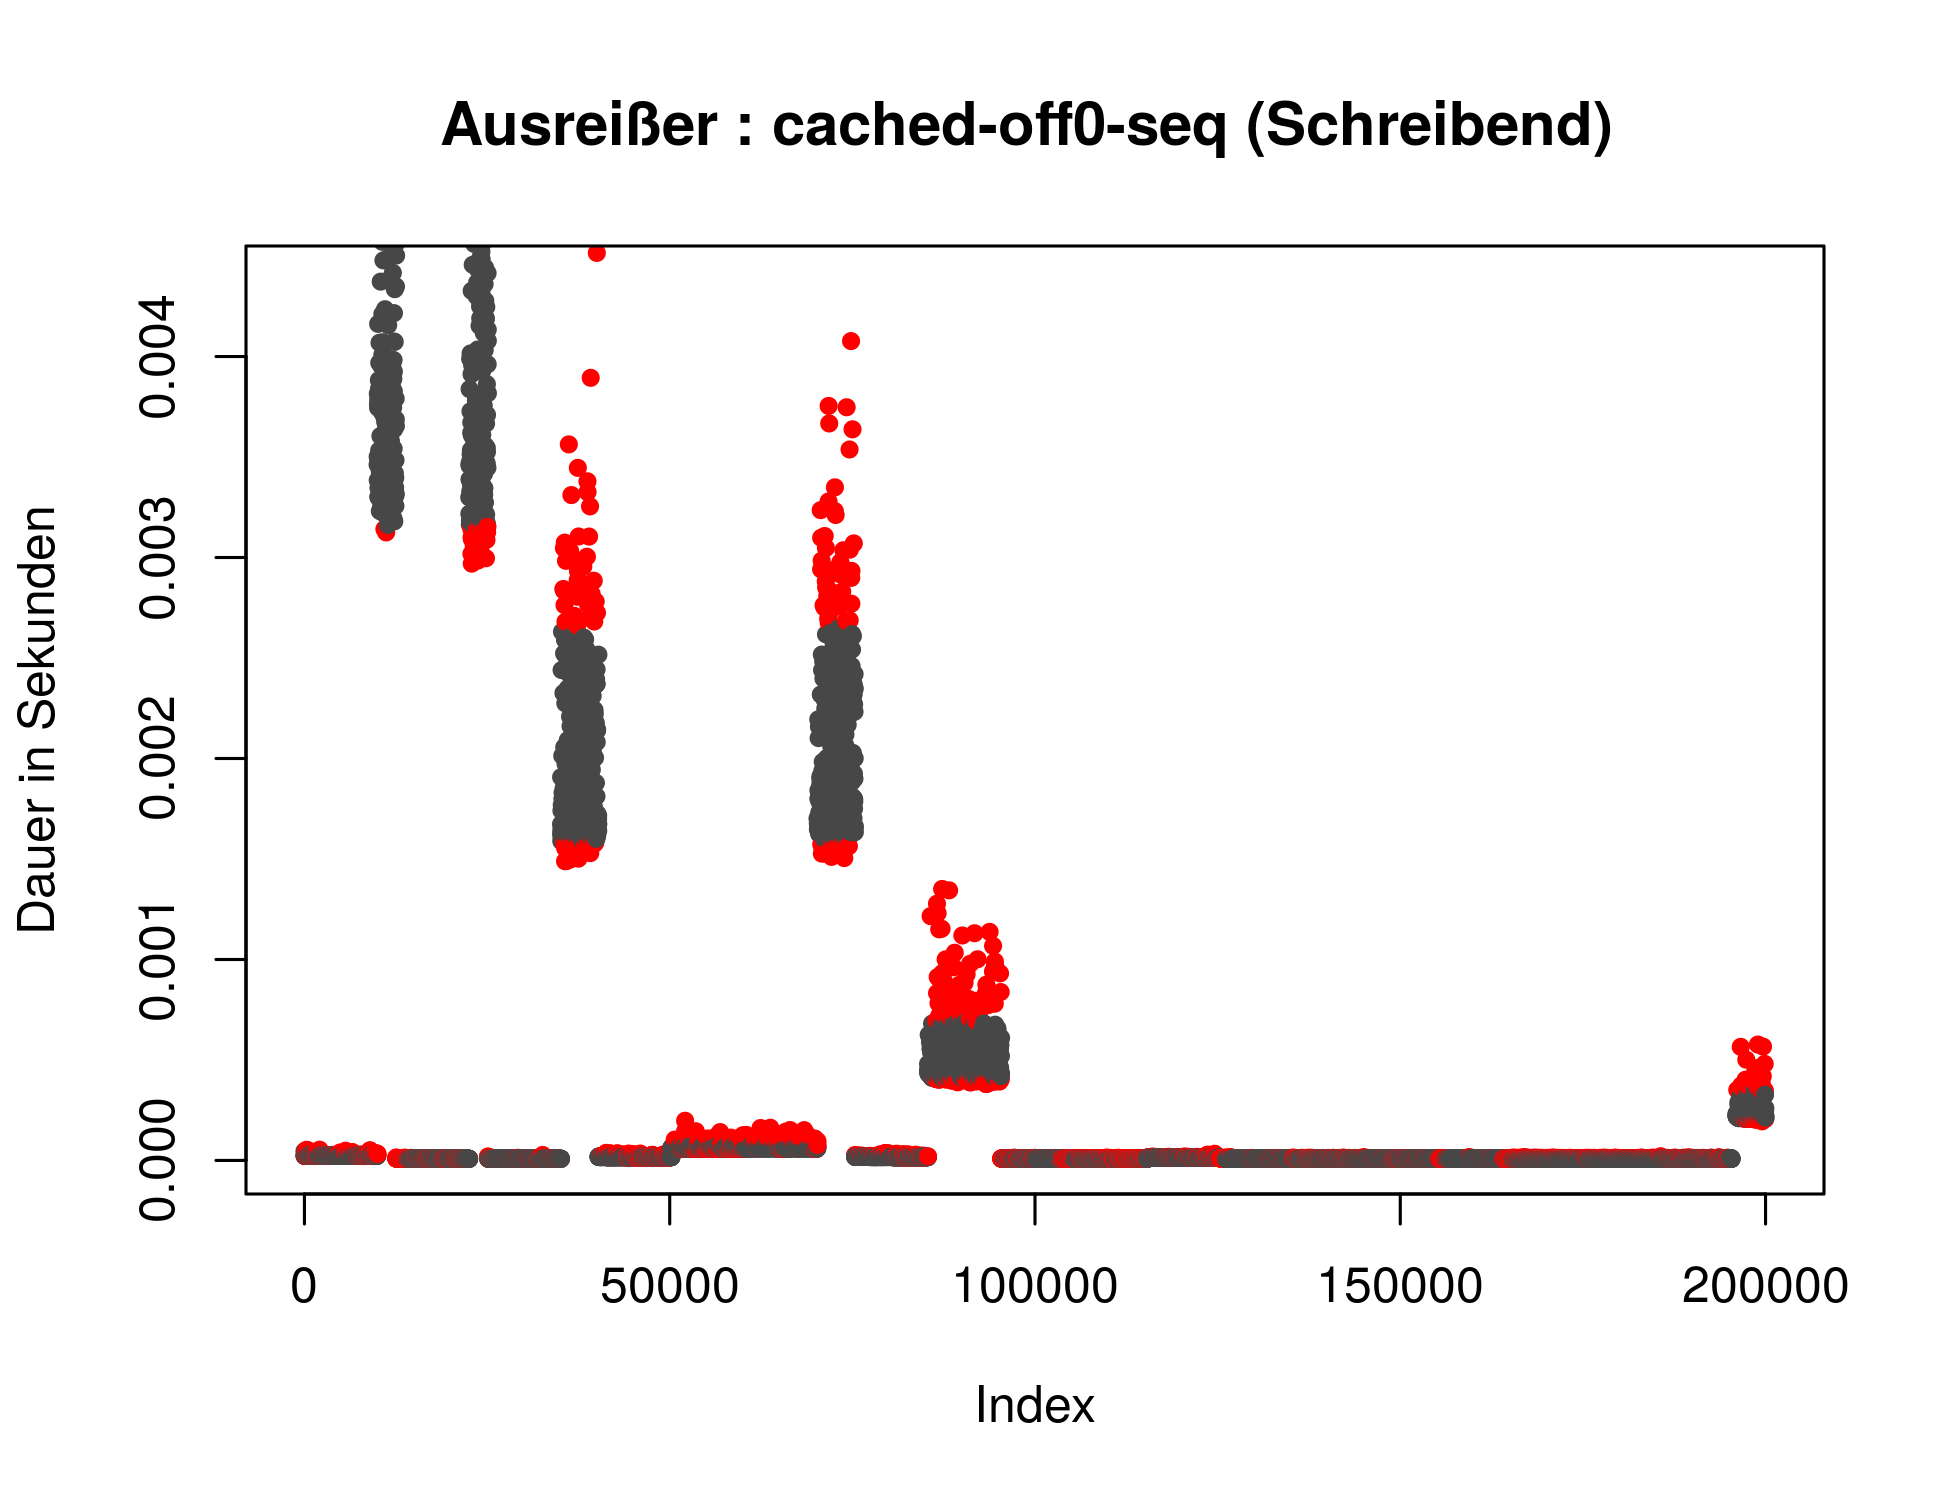
\includegraphics[width=.43\textwidth]{Bilder/Plots/exploration/plot_outlier_write_seq.png}
	}	
	\caption{Ausreißer sind in rot dargstellt}
	\label{fig:ausreisser}
\end{figure} 

\subsubsection{Betrachtung der Laufzeiten pro Zugriffsgröße}
Um die unterschiedlichen Laufzeiten innerhalb einer Zugriffsgröße zu untersuchen, habe ich in den Abbildungen von \ref{fig:groesse1} bis \ref{fig:groesse2097152} für die Größen 1B, 16KiB und 2MiB alle Messungen zu diesen Größen betrachtet.\\
In den Graphen ist gut zu erkennen, dass die Varianz der Laufzeiten im sequentiellen Fall wesentlich geringer ausfällt, als bei den randomisierten Messungen.
Teilweise lassen sich die verschiedenen Messreihen (eine Messreihe umfasst 10000 Messungen, außer im 2MiB Fall, dort sind es 5000) am Muster der Zugriffszeiten voneinander unterscheiden.
So ist beispielsweise eine Verschiebung des Musters bei \ref{fig:groesse16384}c nach 10000 und 20000 Messungen deutlich zu erkennen.
Abhängig vom Systemzustand zum Beginn der Messreihe konnten die Anfragen also im Mittel unterschiedlich schnell bearbeitet werden.
In einigen Bildern lassen sich auch kurzzeitige Maxima oder Minima zwischen den Messreihen feststellen.
Beim sequentiell lesenden Fall für ein Byte (Abbildung \ref{fig:groesse1}a) dauern die ersten Messungen jeweils wesentlich länger, bis sich ein niedriger Wert eingependelt hat. Es könnte sein, dass hier nach einigen Zugriffen die Read-Ahead Caching-Strategie greift, die geforderten Daten befinden sich dann im Moment der Anfrage bereits im Cache. Dies macht auch Sinn, da der sequentielle Zugriff sehr gut vorhersagbar ist.\\
Für die randomisierten Datensätze ist ein solches Verhalten nicht möglich und kann auch in keiner Abbildung erkannt werden.\\
Ein interessantes Verhalten kann in Abbildung \ref{fig:groesse16384}a beobachtet werden.
Zu Beginn jeder Messerreihe werden die ersten E/A-Zugriffe zuverlässig sehr schnell ausgeführt, dann steigt die mittlere Zugriffszeit rapide an und oszilliert stark.
Möglicherweise wird in diesem Fall solange der Arbeitsspeicher aufgefüllt, bis der Platz nicht mehr ausreicht und aufwendigere Speicherverwaltungen Platz für die neuen Daten im Speicher schaffen müssen.

\begin{figure}
	\subfloat[Messungen mit Zugriffsgröße 1B auf SEQ-R]{
		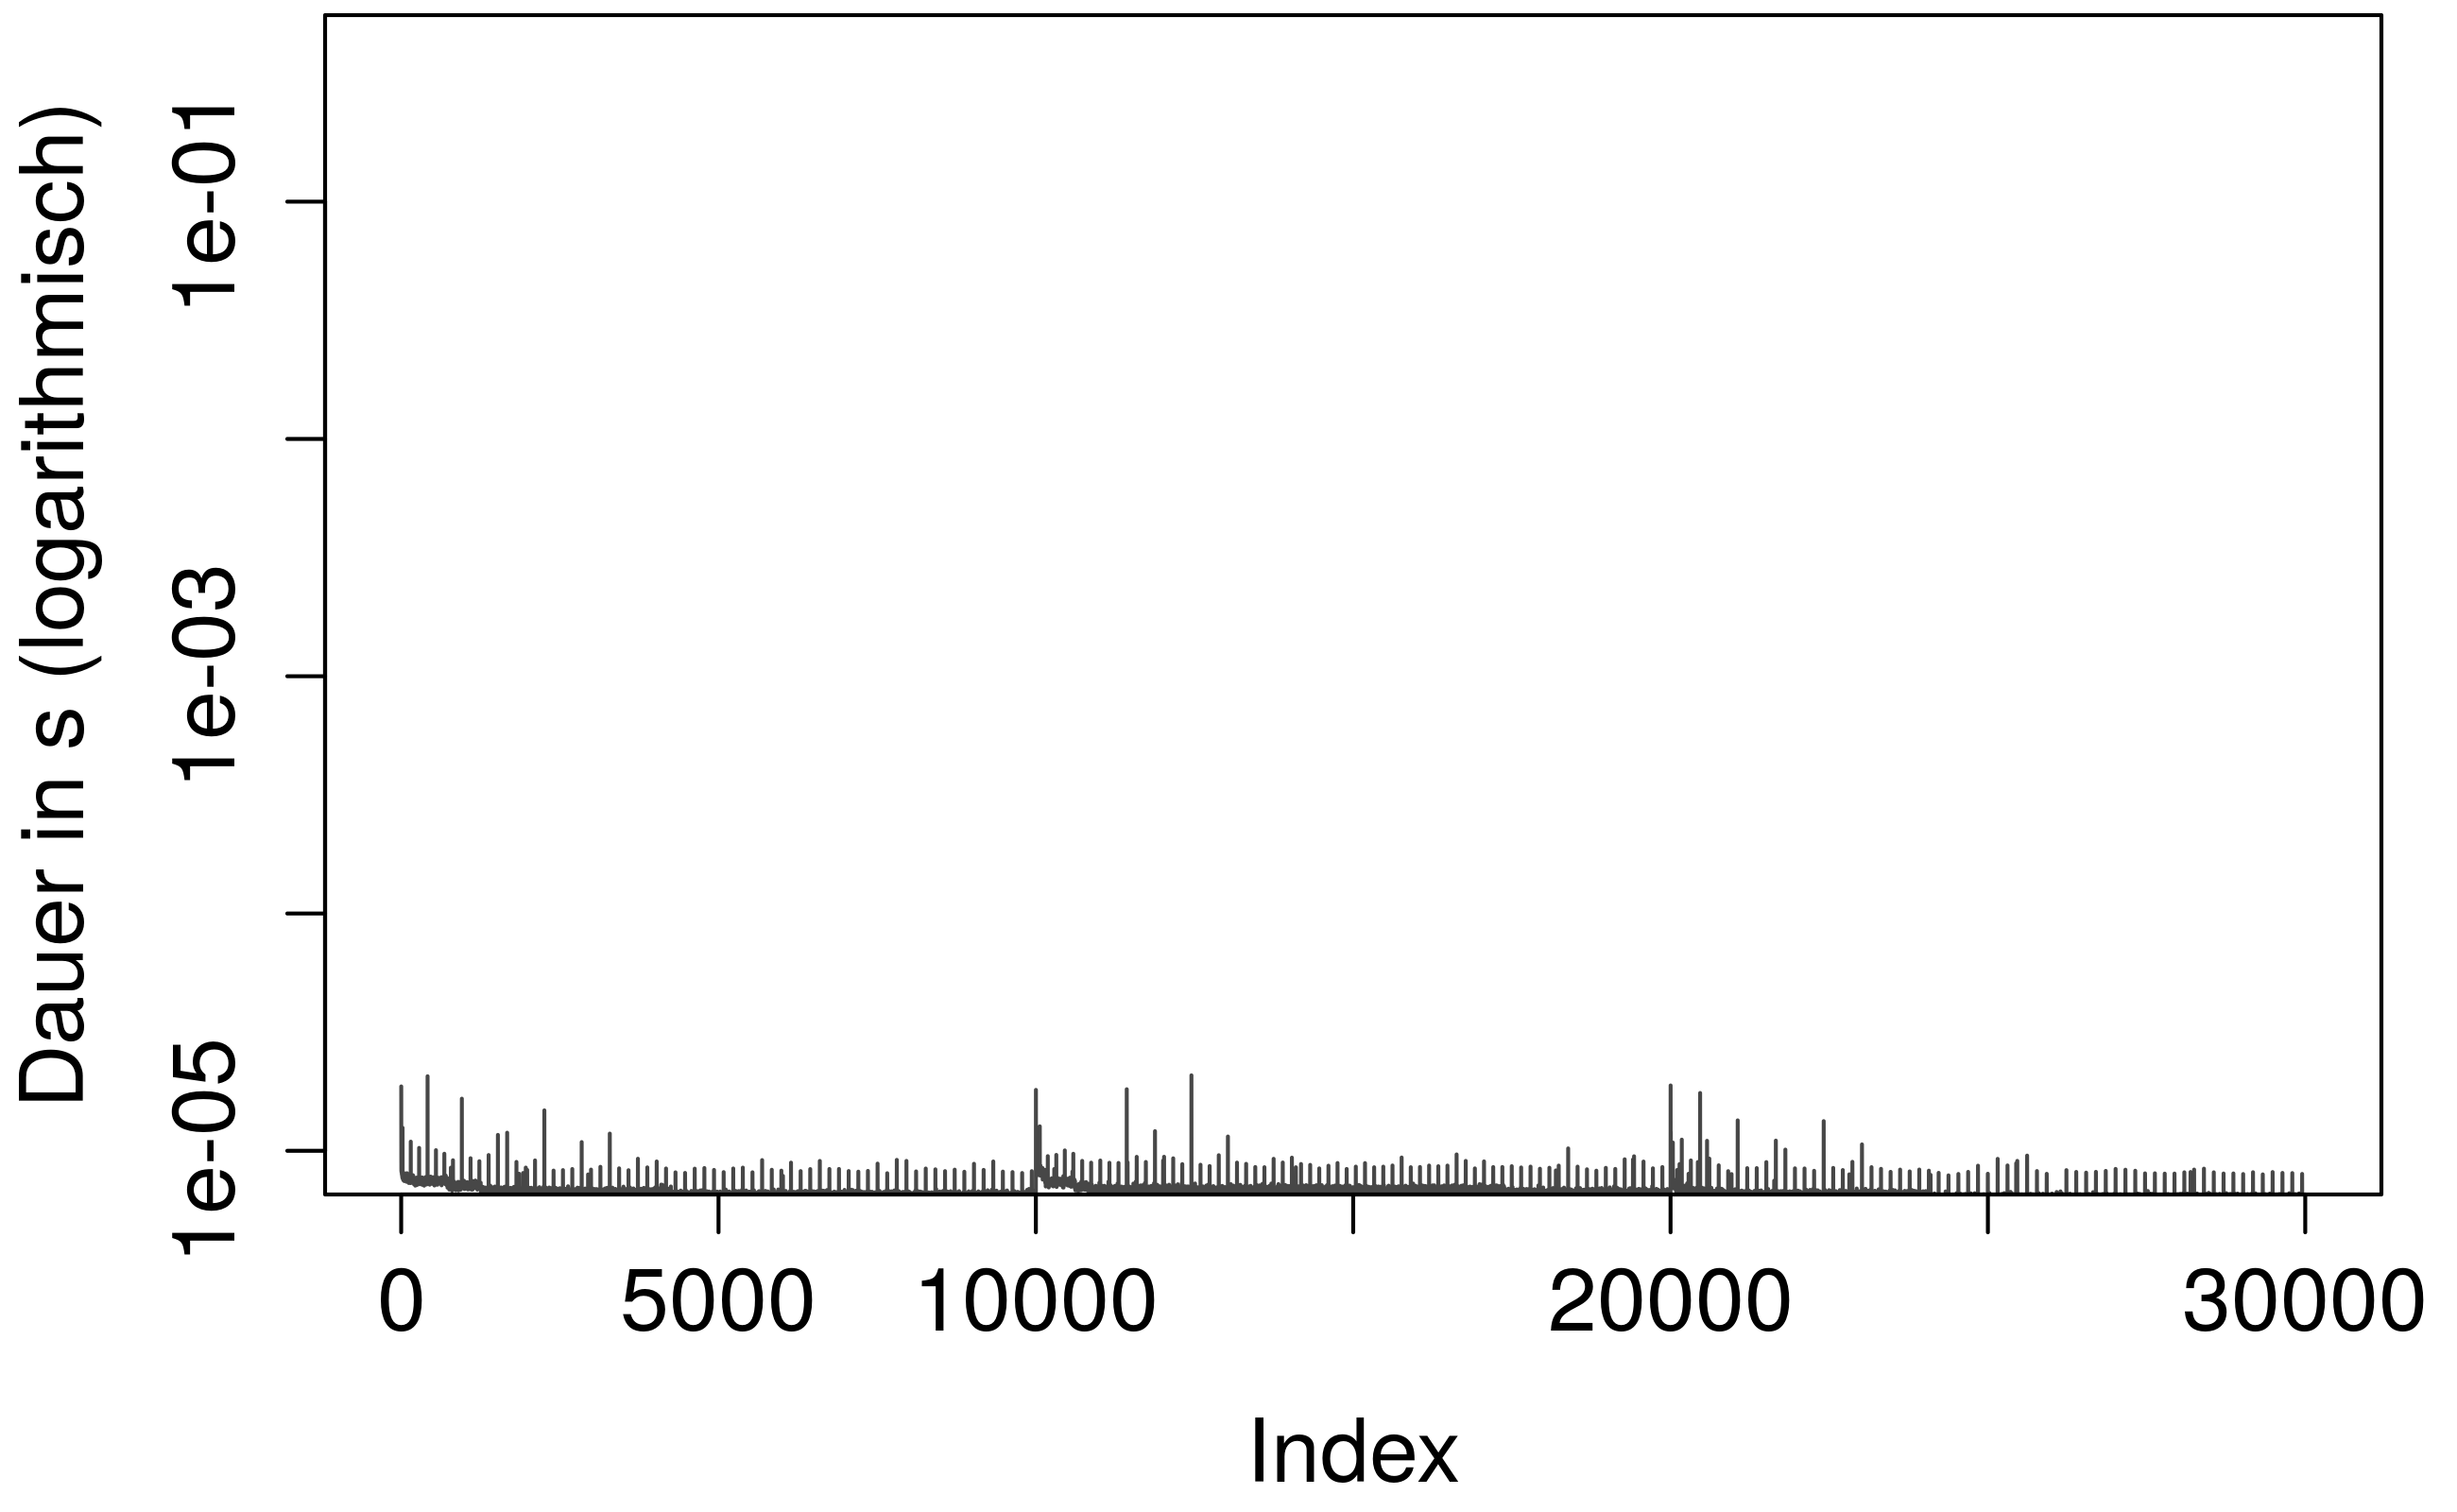
\includegraphics[width=.43\textwidth]{Bilder/Plots/exploration/plot_Size1_read_seq.png}
	}
	\hfill
	\subfloat[Messungen mit Zugriffsgröße 1B auf SEQ-W]{
		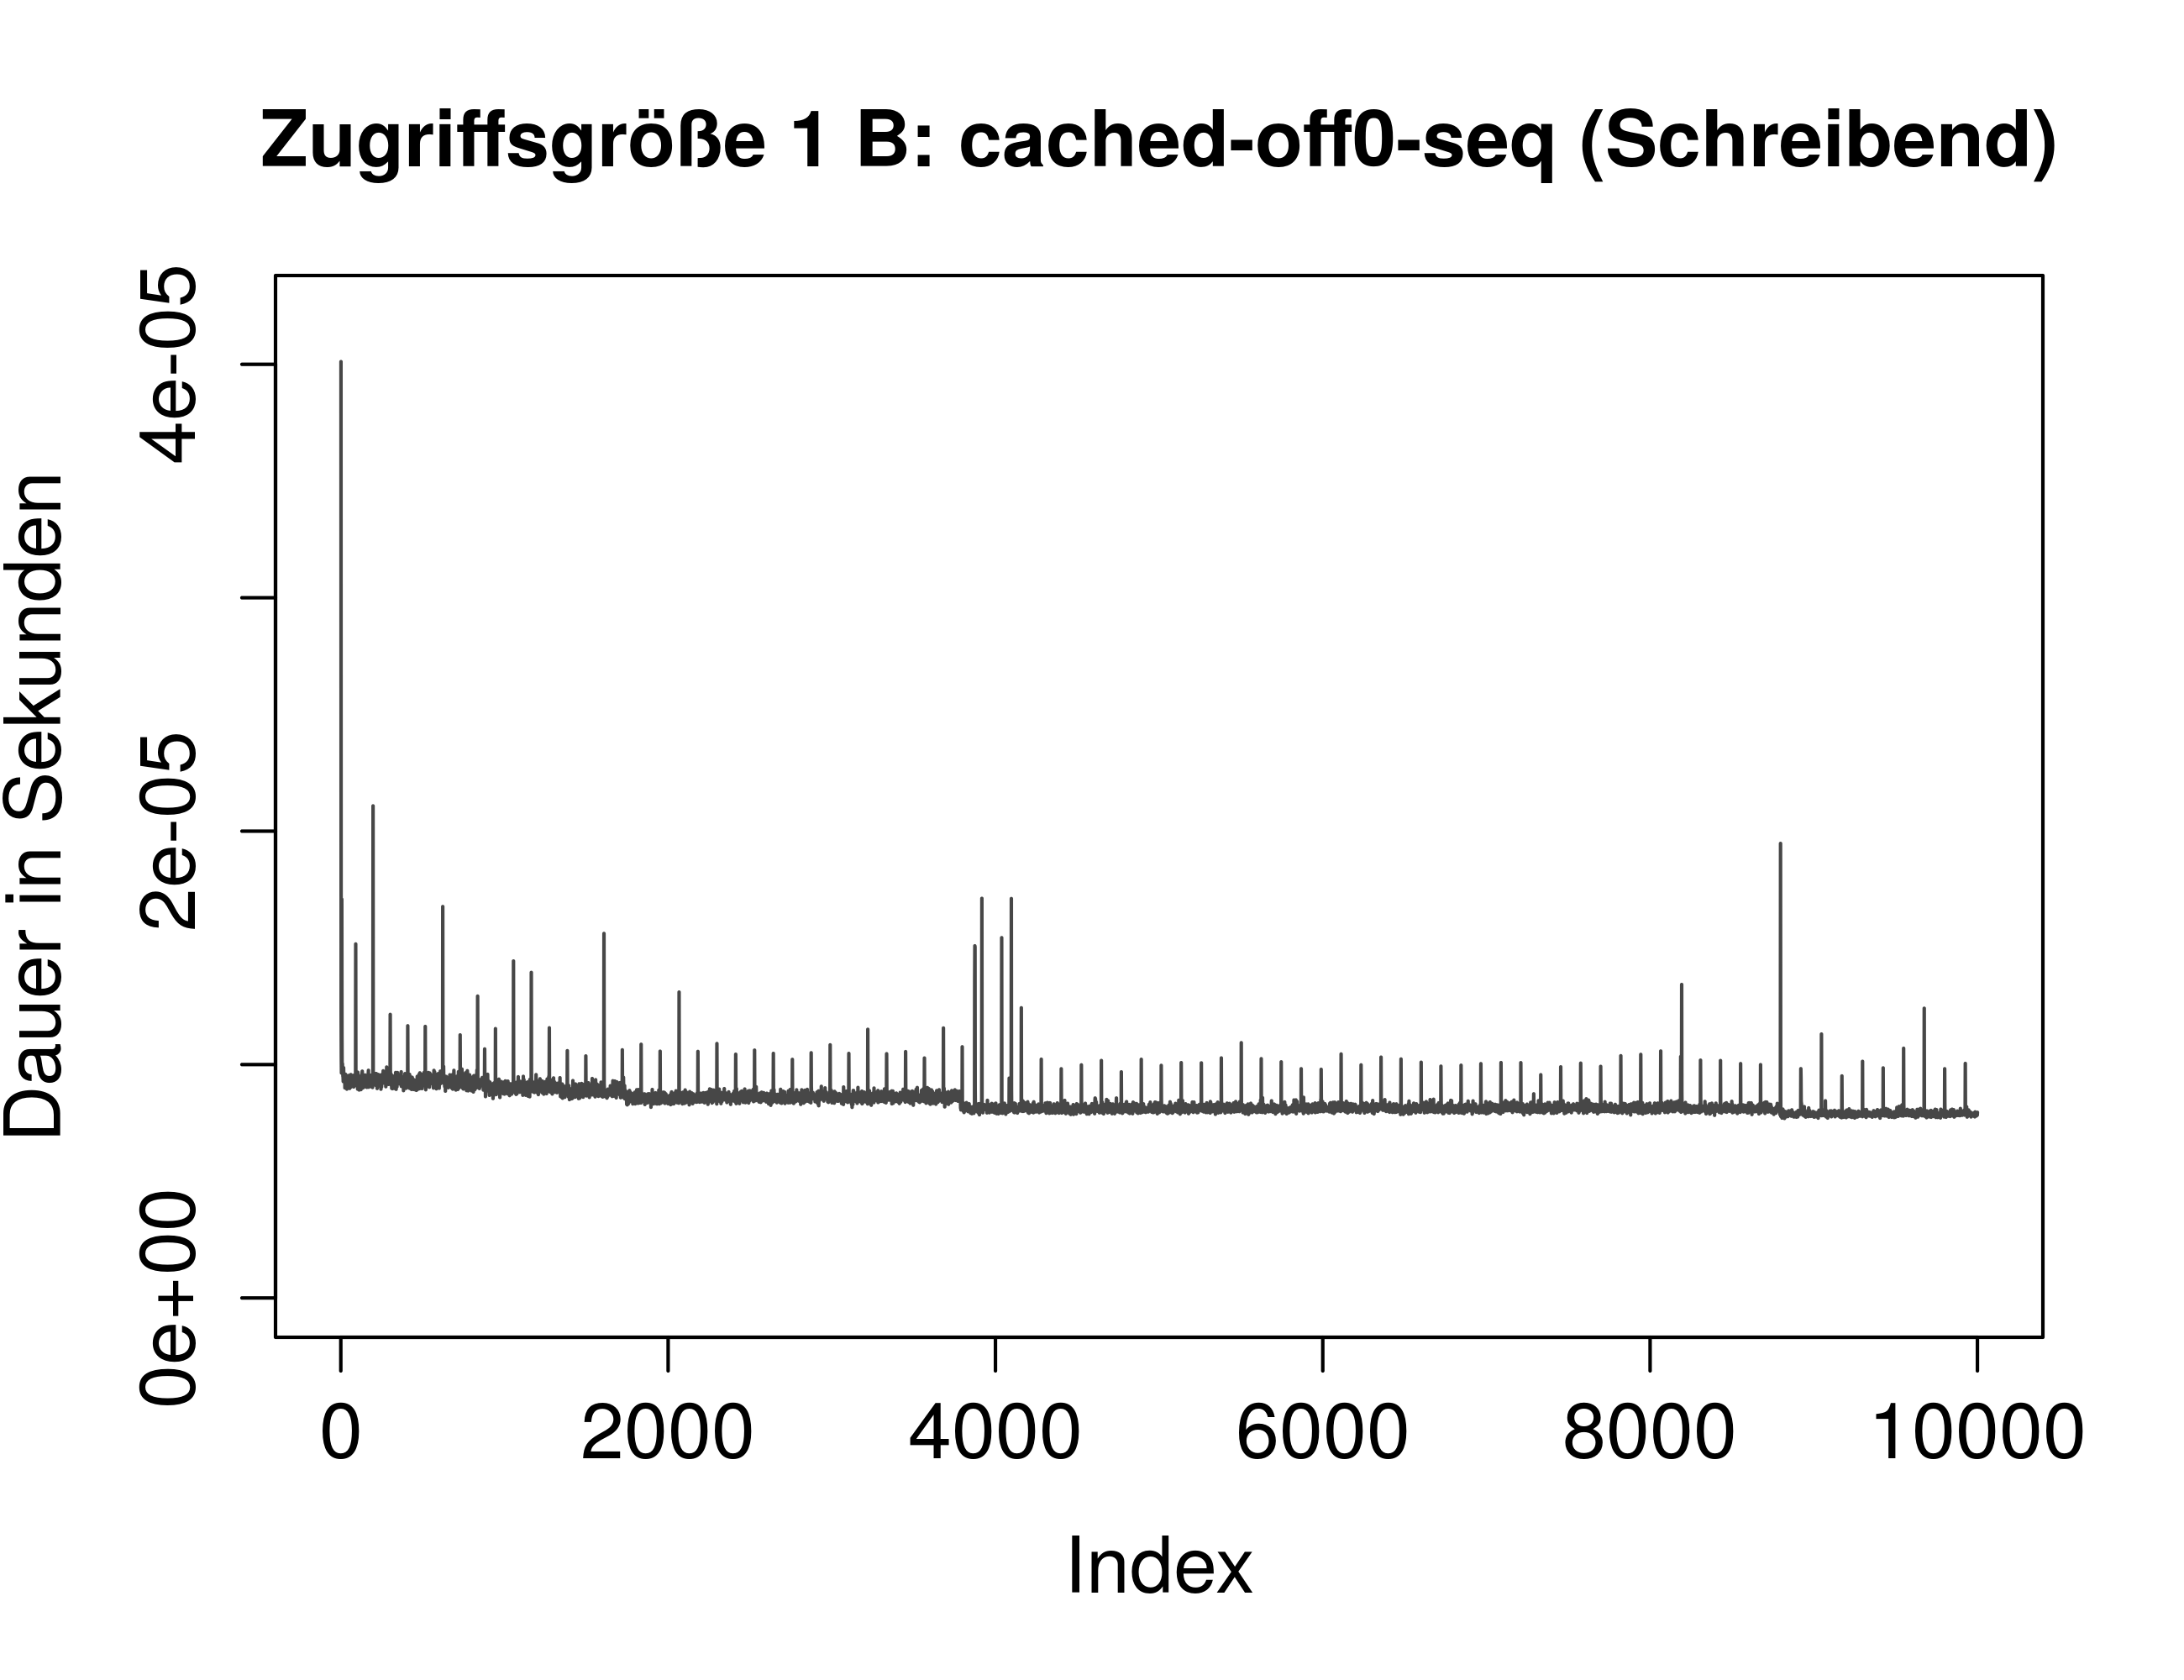
\includegraphics[width=.43\textwidth]{Bilder/Plots/exploration/plot_Size1_write_seq.png}
	}\\
	\subfloat[Messungen mit Zugriffsgröße 1B auf RND-R]{
		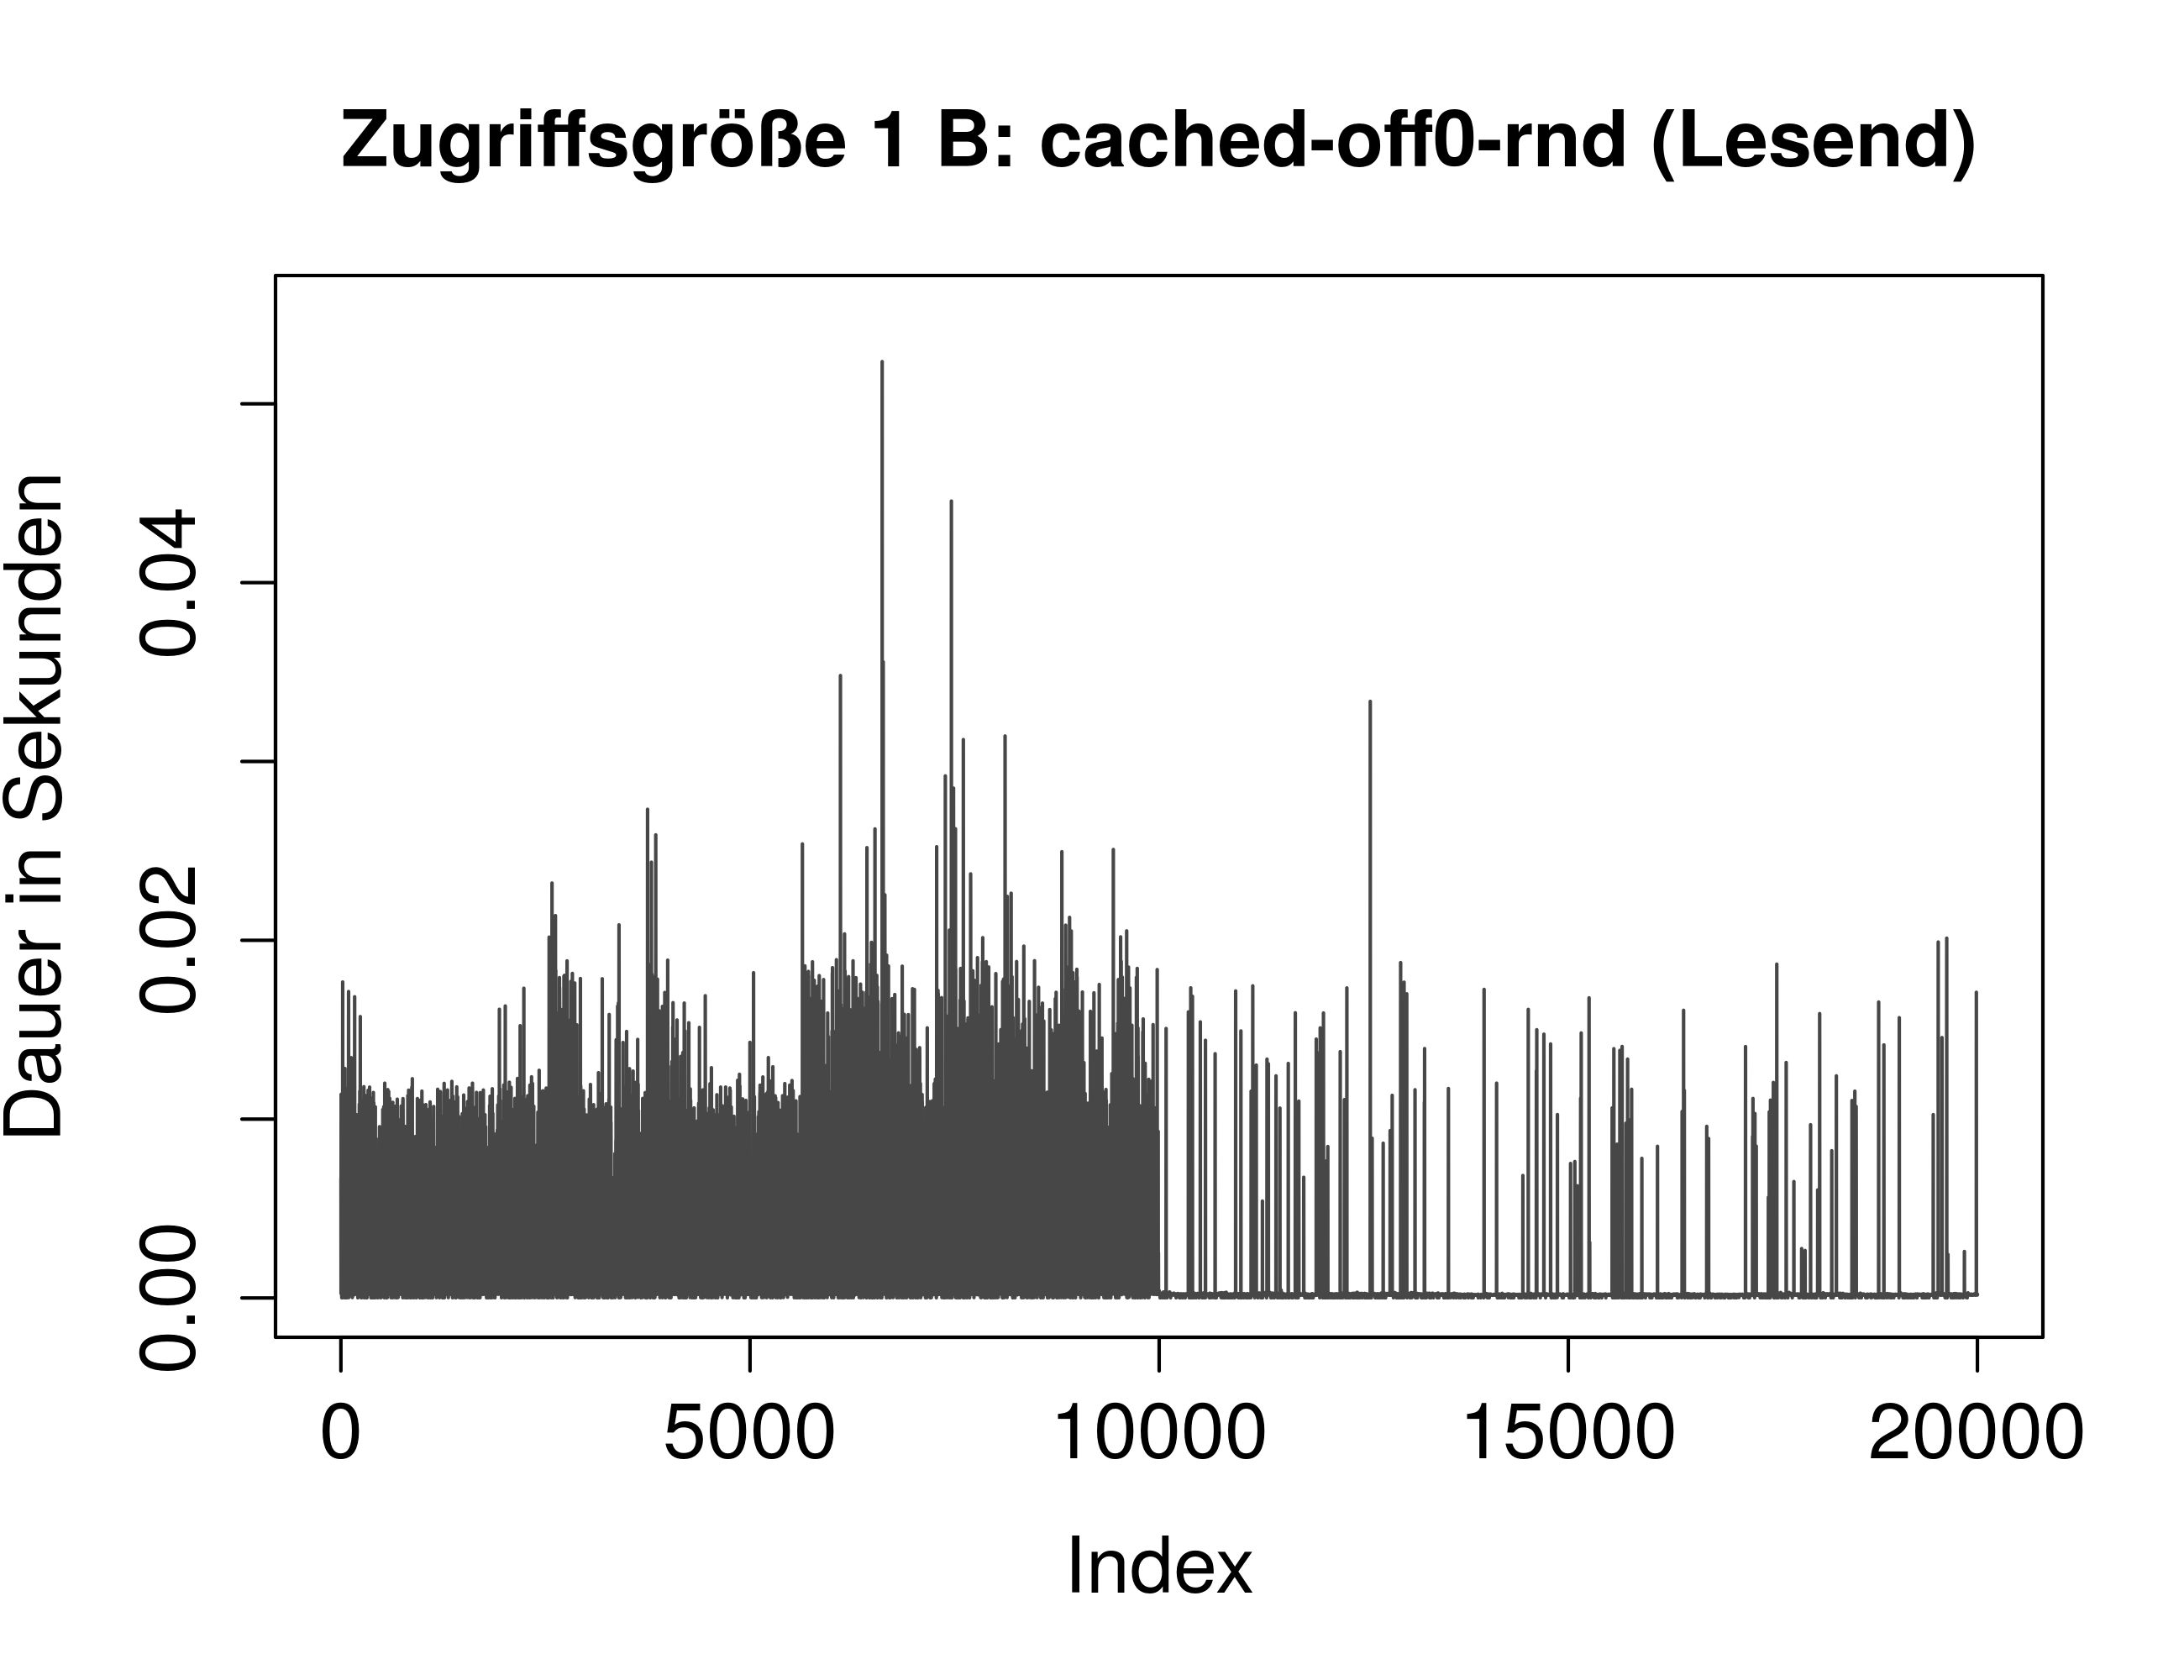
\includegraphics[width=.43\textwidth]{Bilder/Plots/exploration/plot_Size1_read_rnd.png}
	}
	\hfill
	\subfloat[Messungen mit Zugriffsgröße 1B auf RND-W]{
		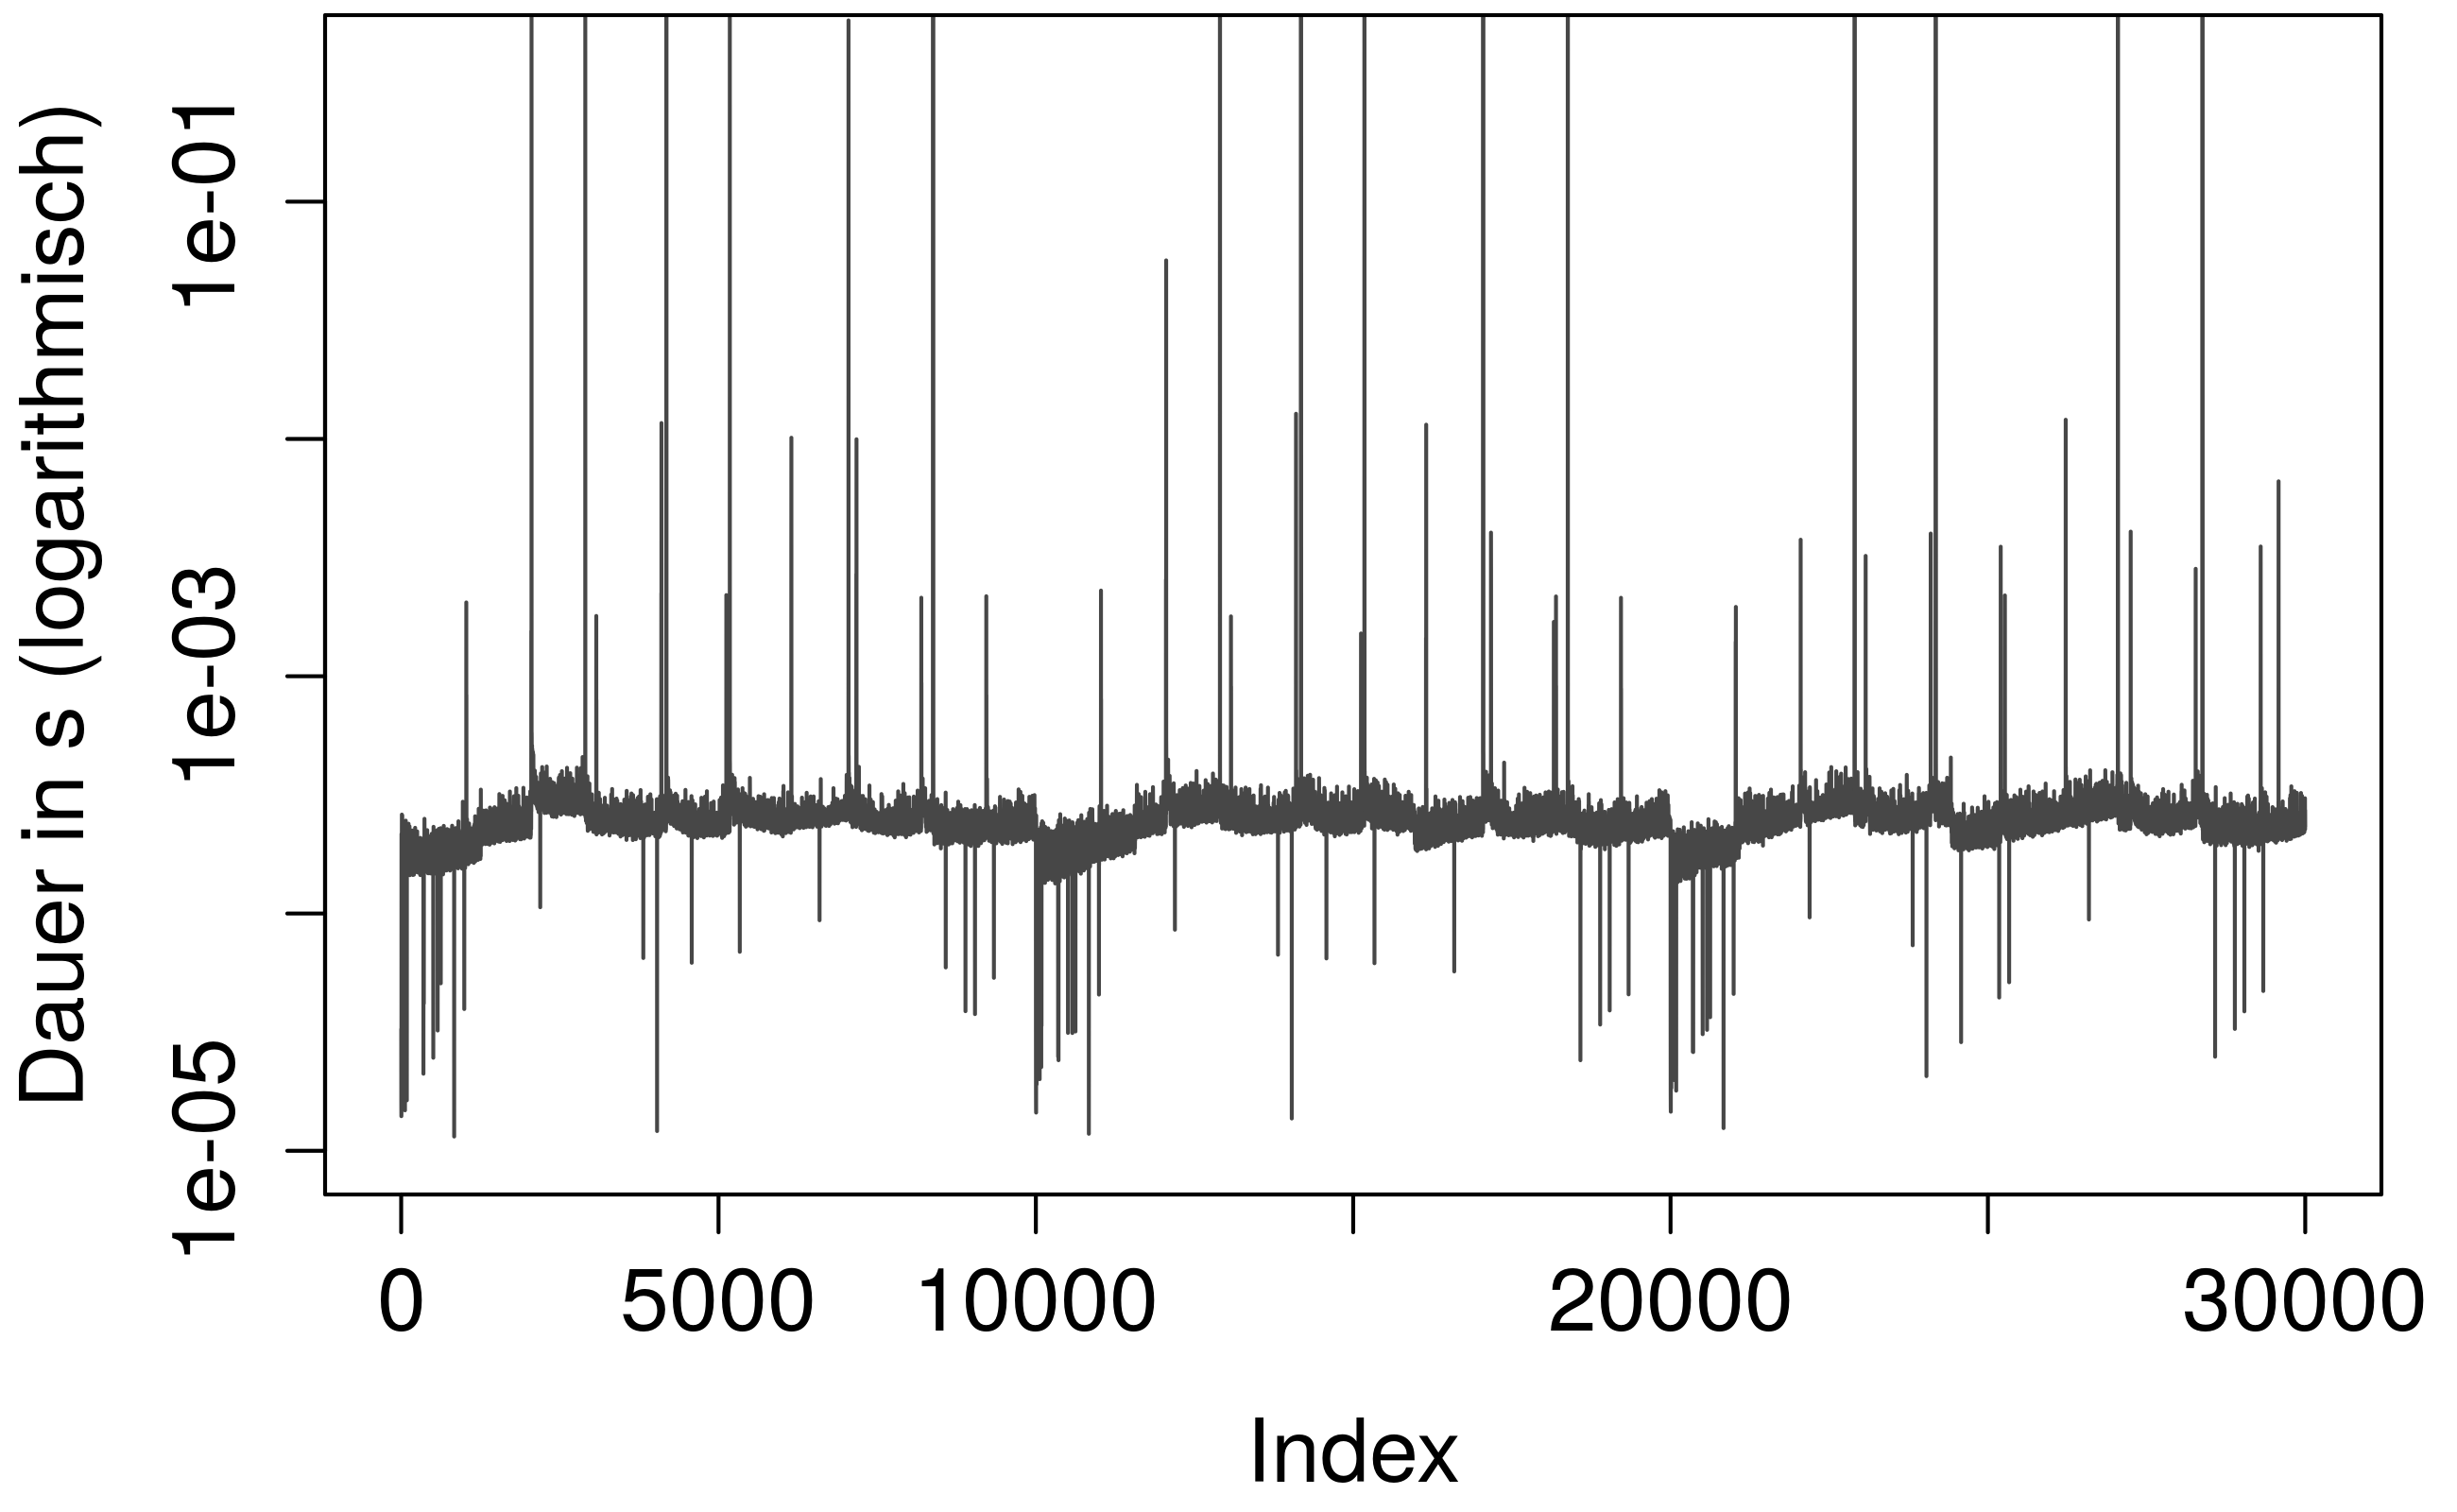
\includegraphics[width=.43\textwidth]{Bilder/Plots/exploration/plot_Size1_write_rnd.png}
	}		
	\caption{Detailbetrachtung aller Messungen mit Zugriffsgröße 1B}
	\label{fig:groesse1}
\end{figure}
\begin{figure}
	\subfloat[Messungen mit Zugriffsgröße 16KiB auf SEQ-R]{
		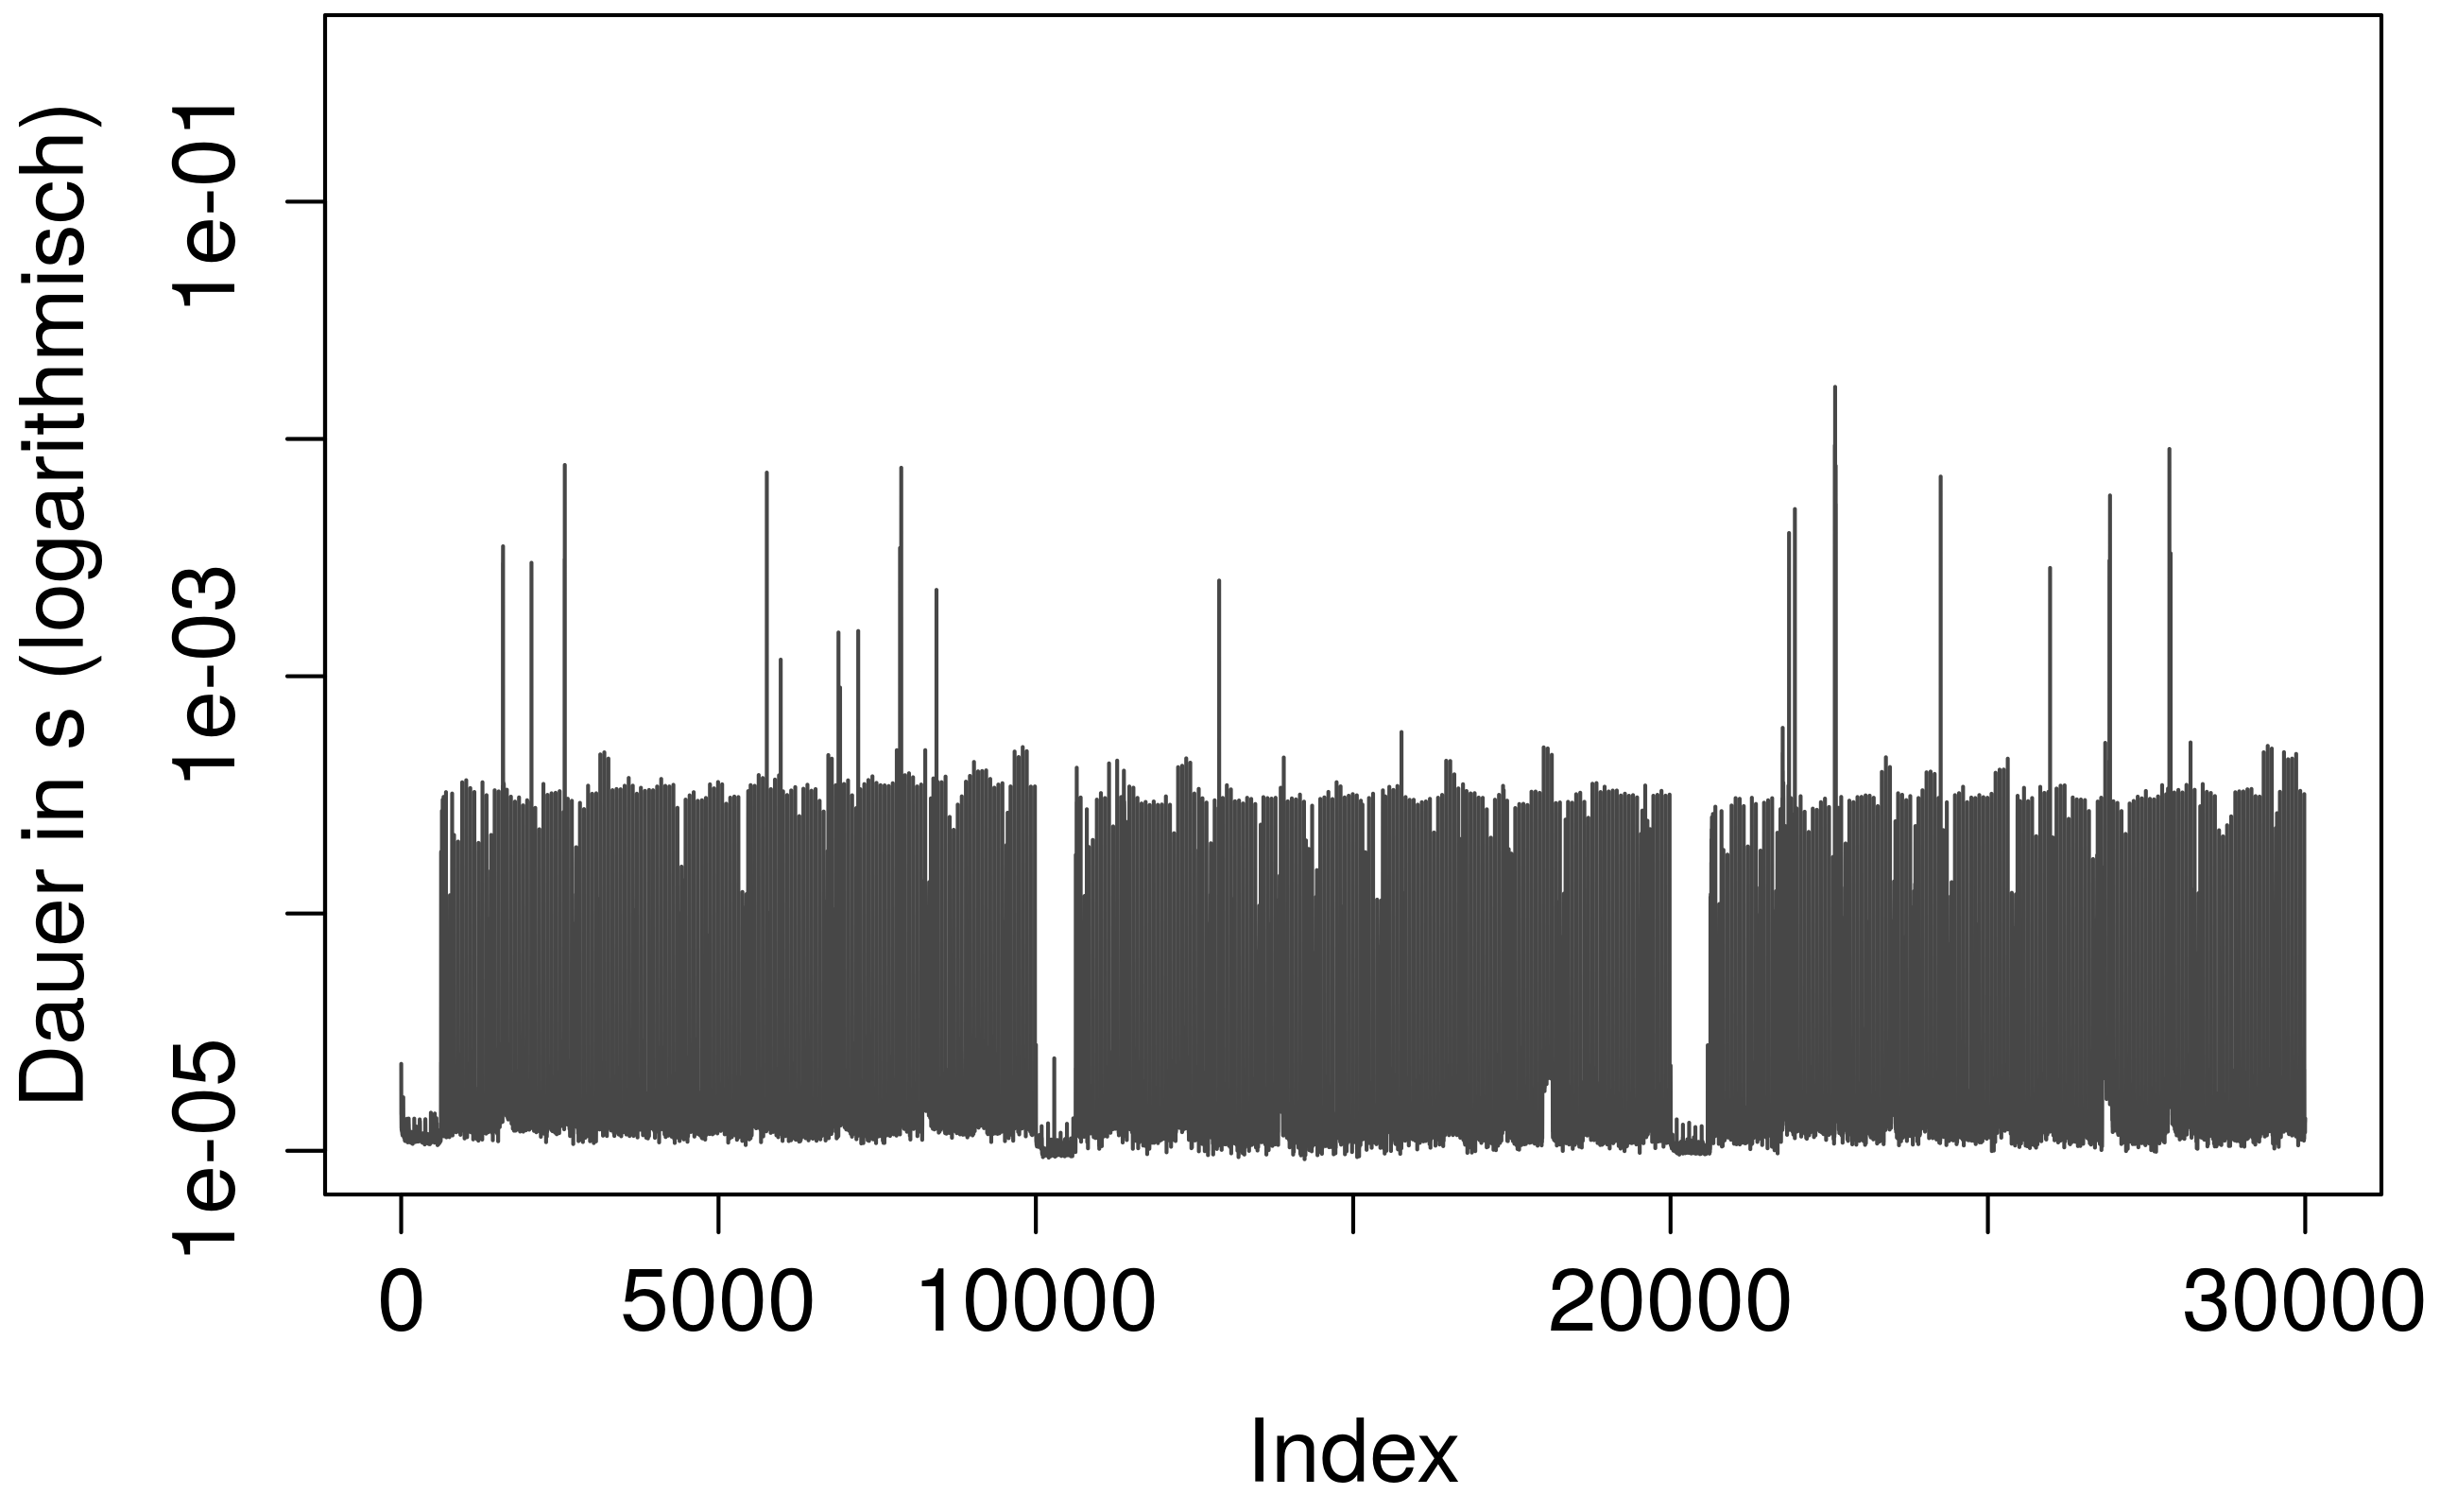
\includegraphics[width=.43\textwidth]{Bilder/Plots/exploration/plot_Size16384_read_seq.png}
	}
	\hfill
	\subfloat[Messungen mit Zugriffsgröße 16KiB auf SEQ-W]{
		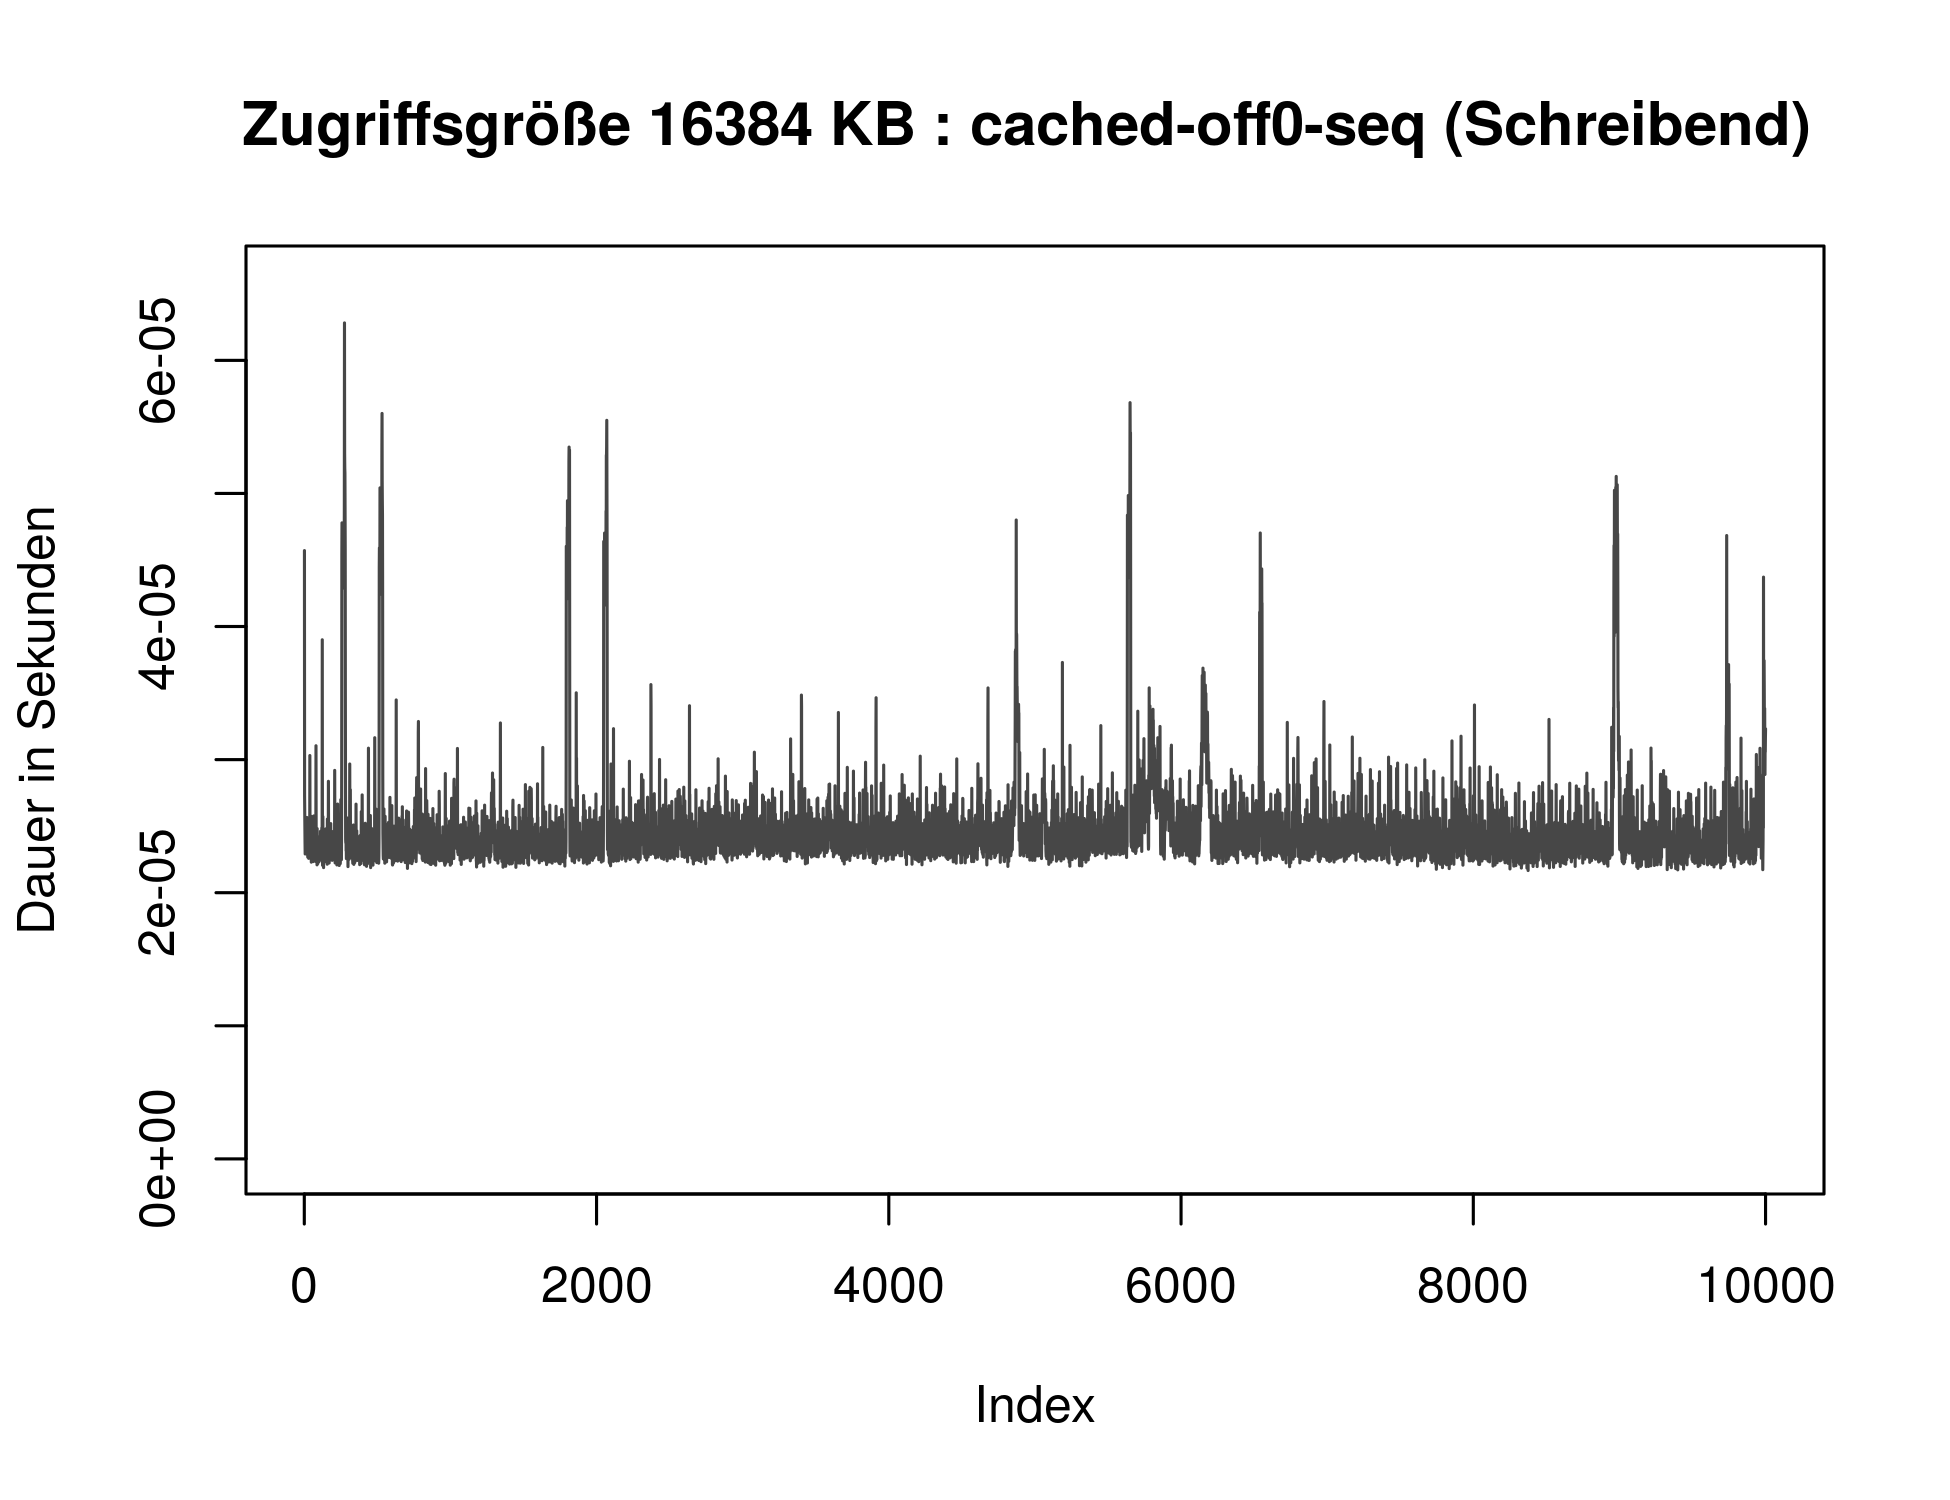
\includegraphics[width=.43\textwidth]{Bilder/Plots/exploration/plot_Size16384_write_seq.png}
	}\\
	\subfloat[Messungen mit Zugriffsgröße 16KiB auf RND-R]{
		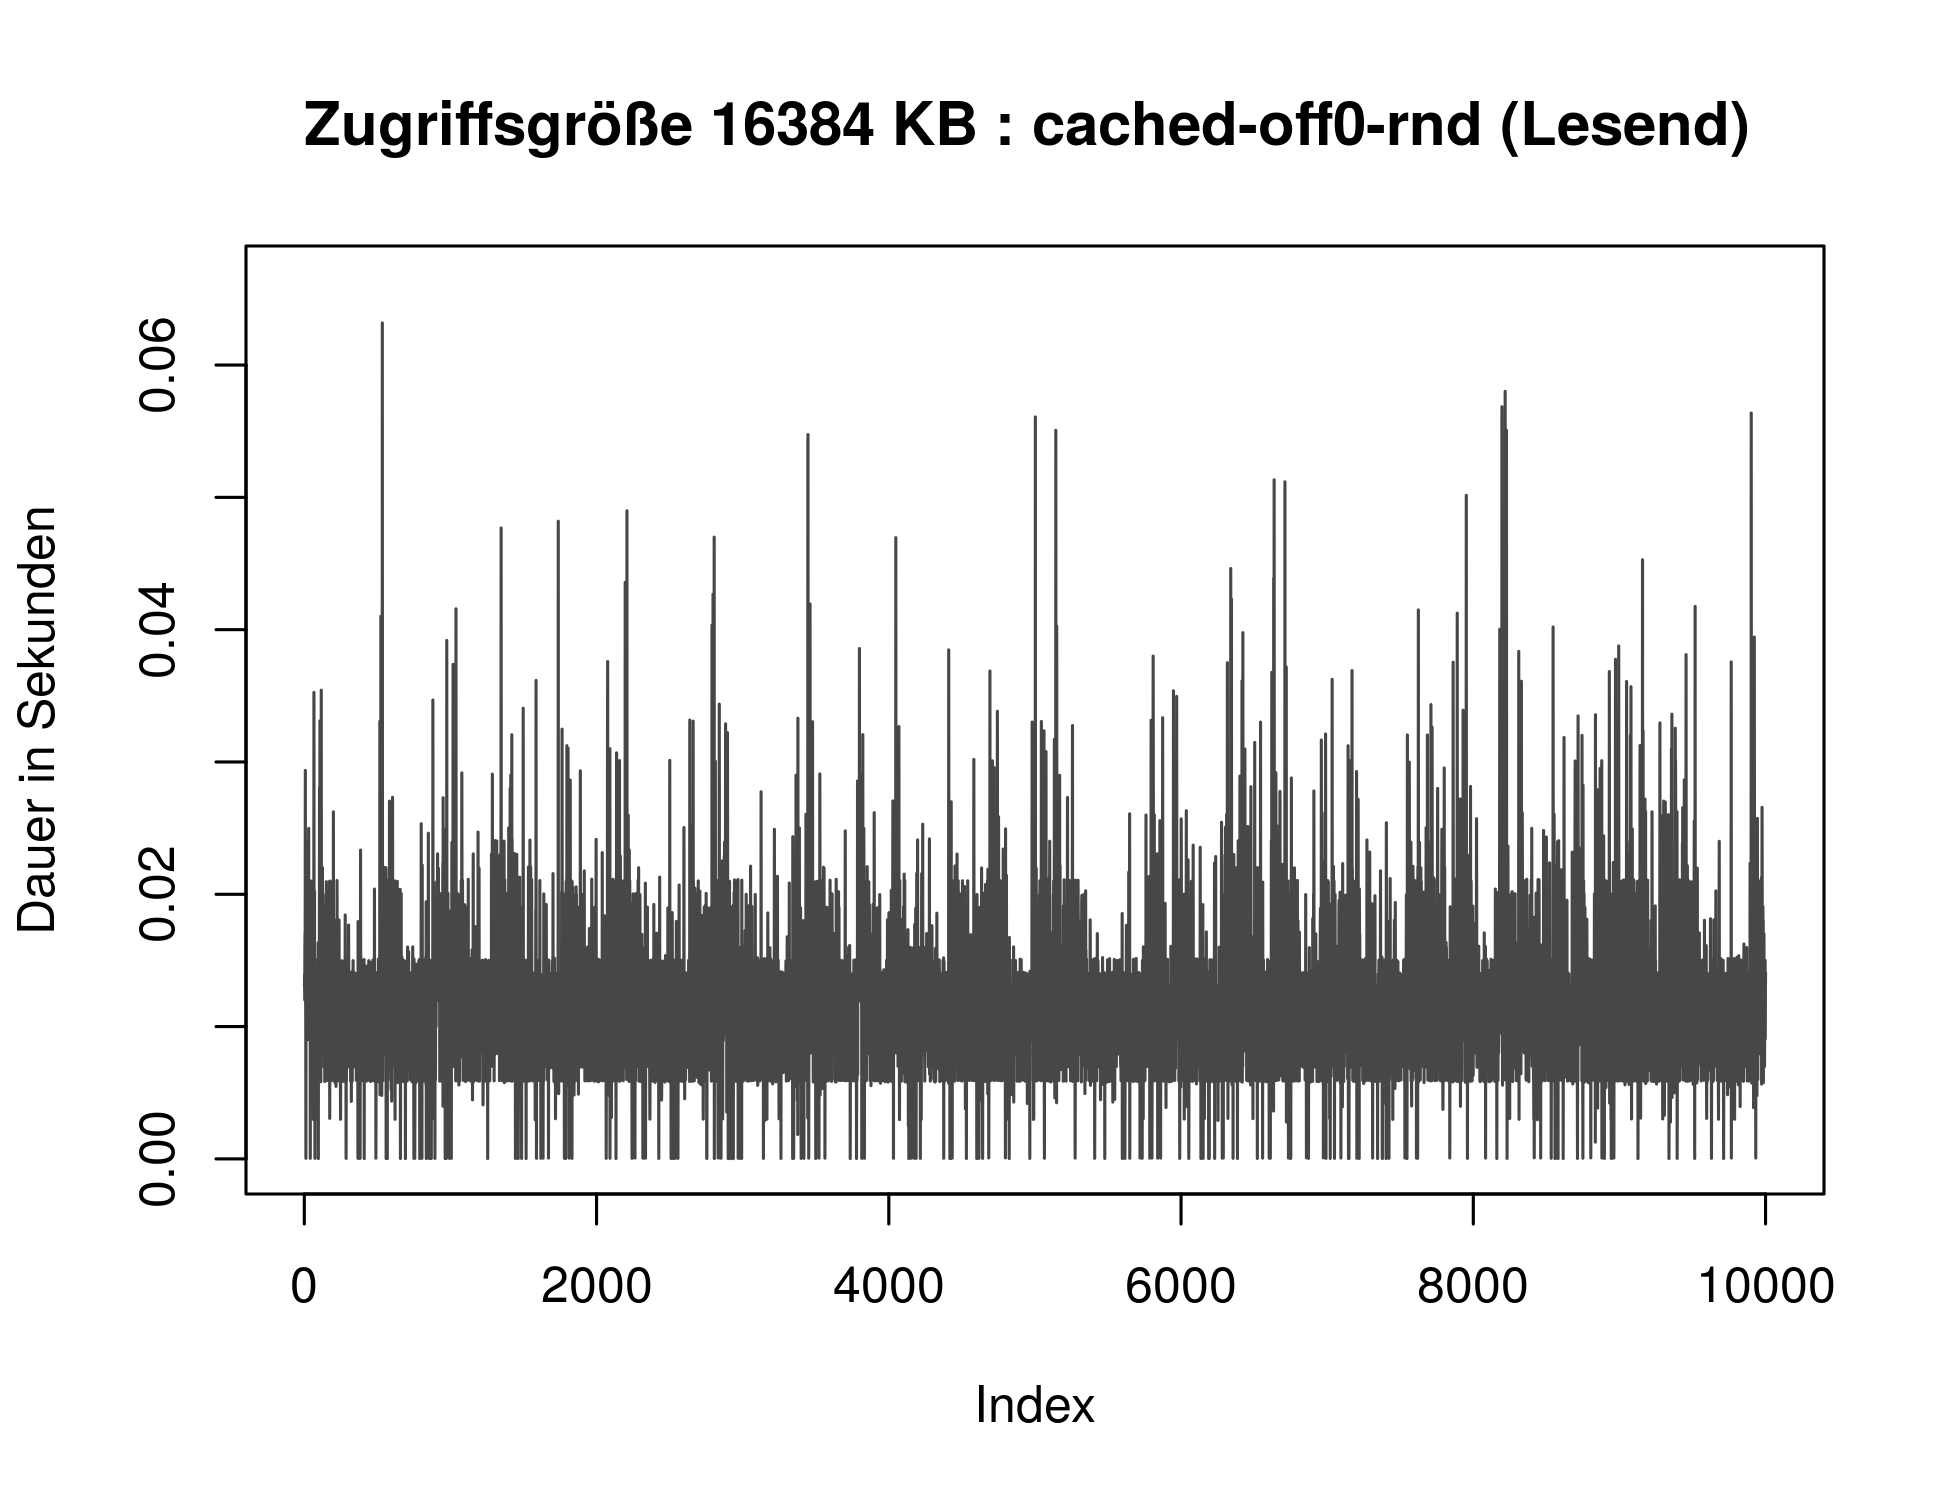
\includegraphics[width=.43\textwidth]{Bilder/Plots/exploration/plot_Size16384_read_rnd.png}
	}
	\hfill
	\subfloat[Messungen mit Zugriffsgröße 16KiB auf RND-W]{
		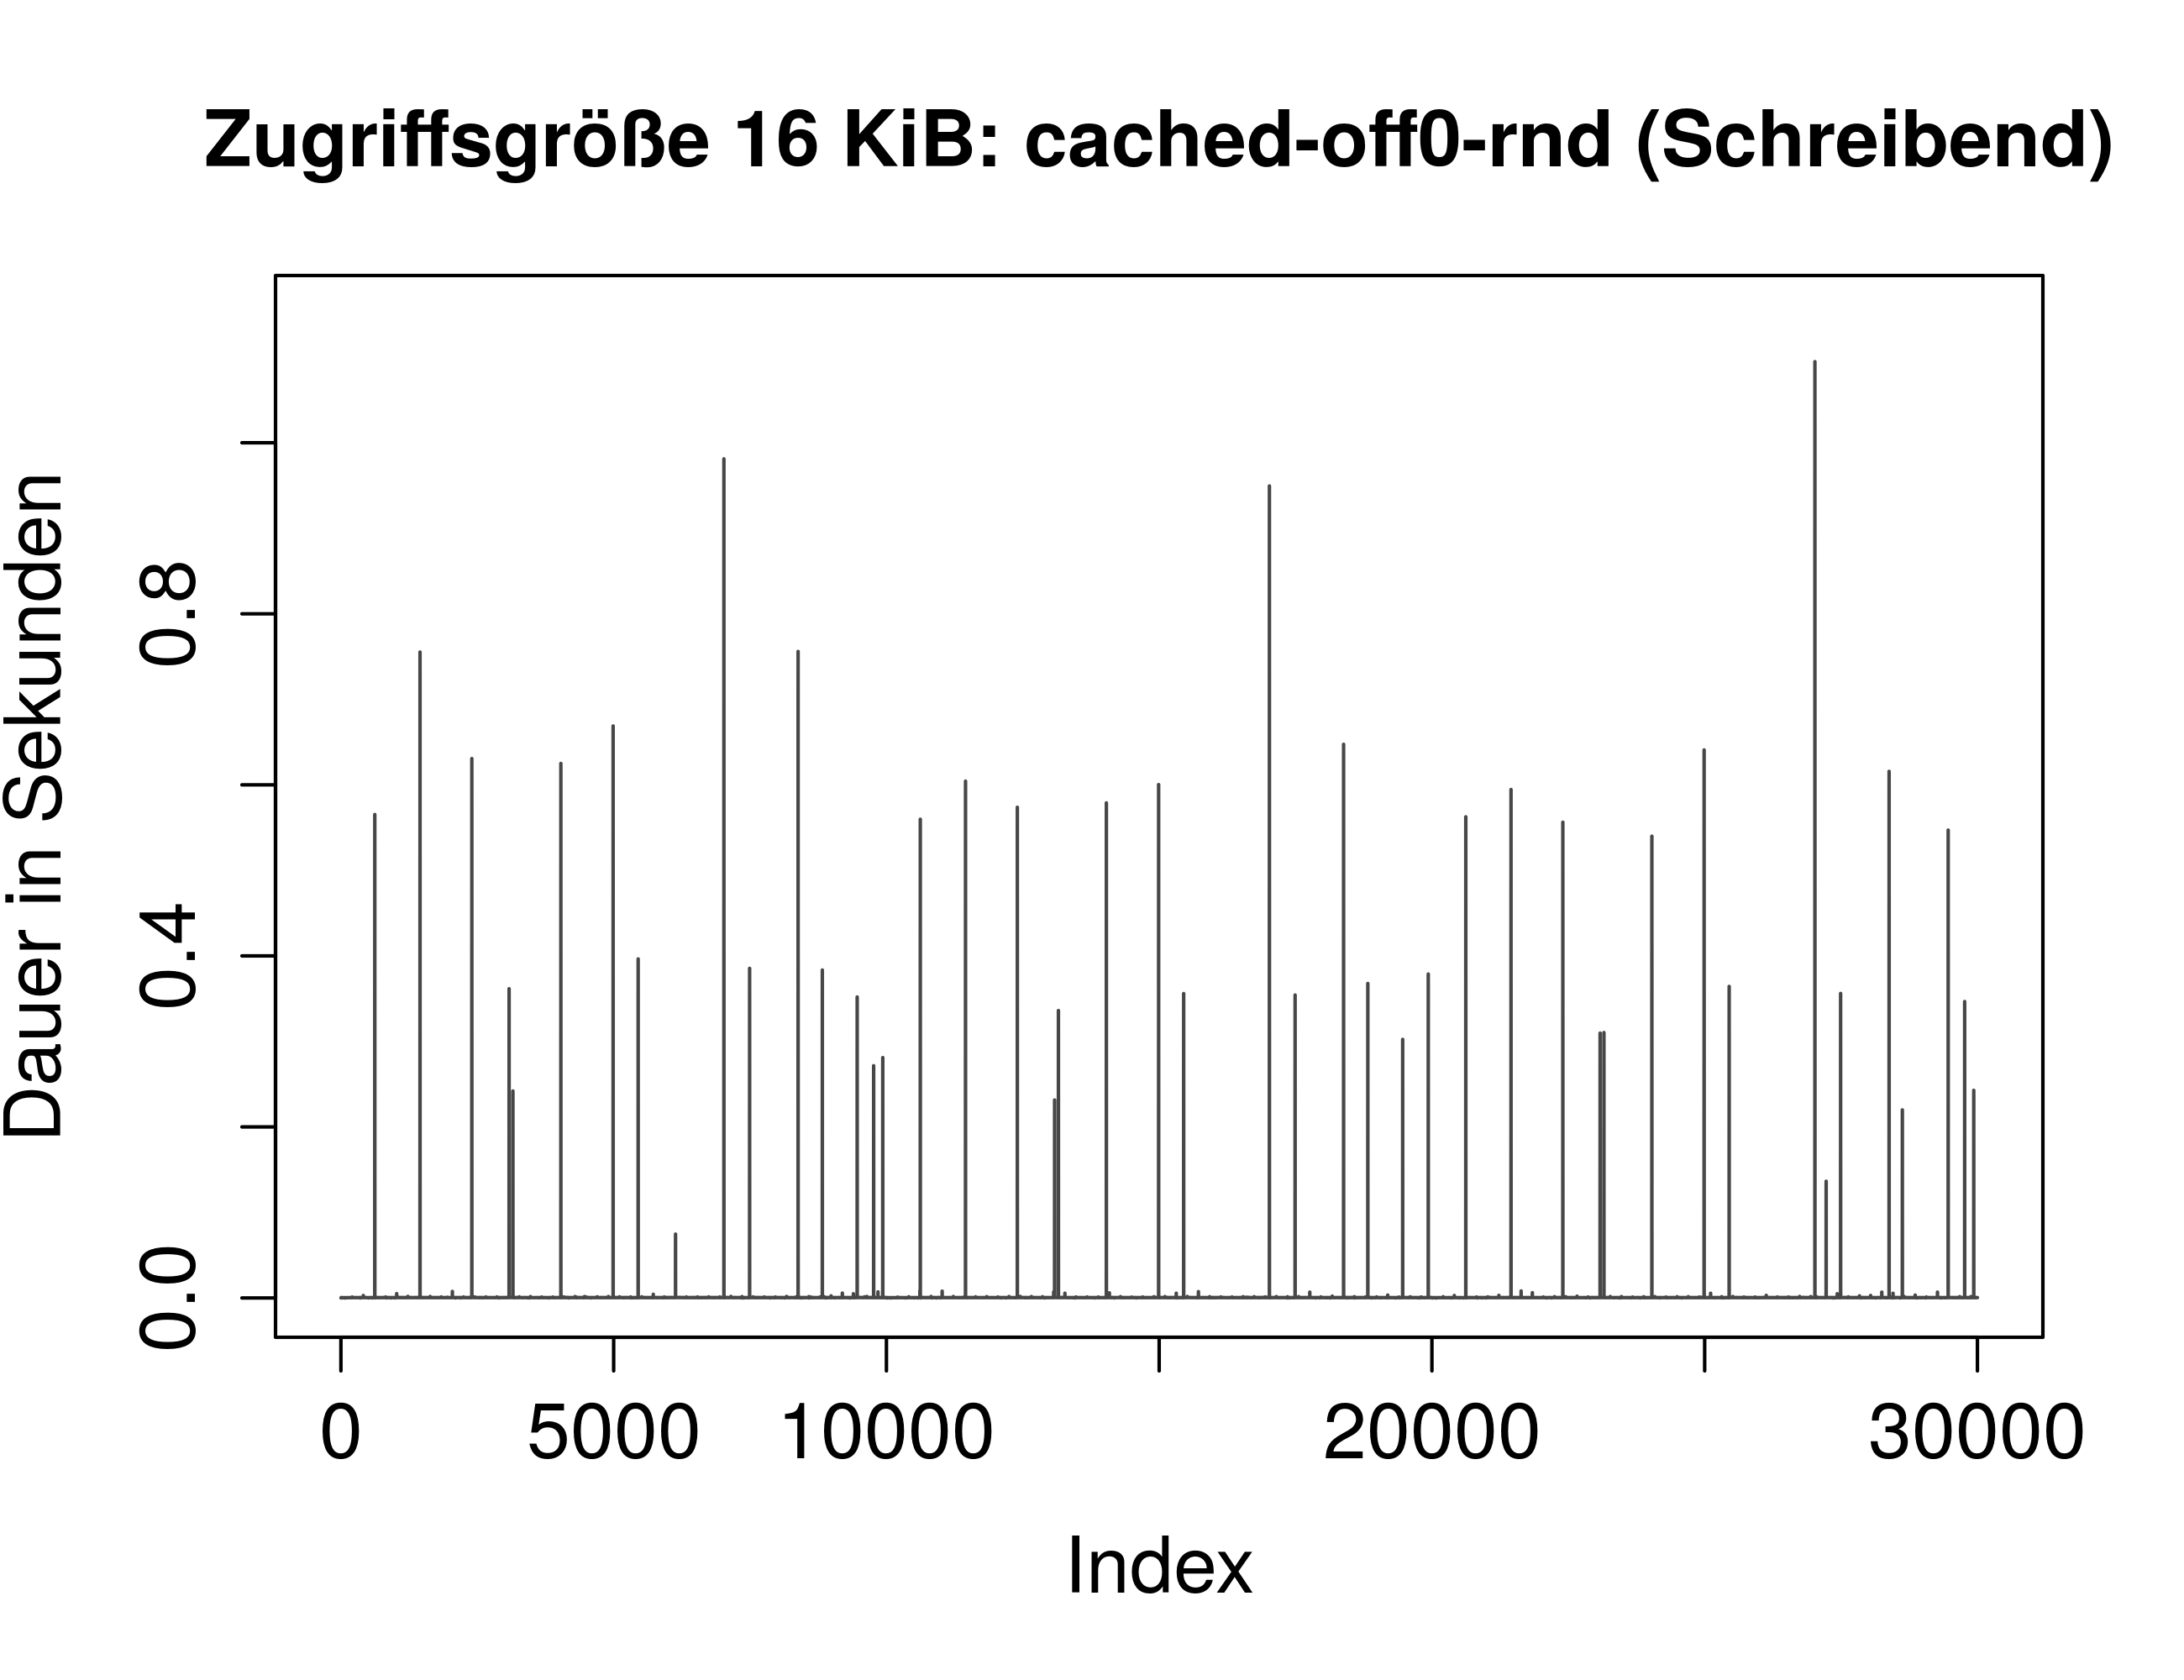
\includegraphics[width=.43\textwidth]{Bilder/Plots/exploration/plot_Size16384_write_rnd.png}
	}		
	\vspace*{-0.3cm}
	\caption{Detailbetrachtung aller Messungen mit Zugriffsgröße 16KiB}
	\label{fig:groesse16384}
\end{figure}
\begin{figure}
	\subfloat[Messungen mit Zugriffsgröße 2MiB auf SEQ-R]{
		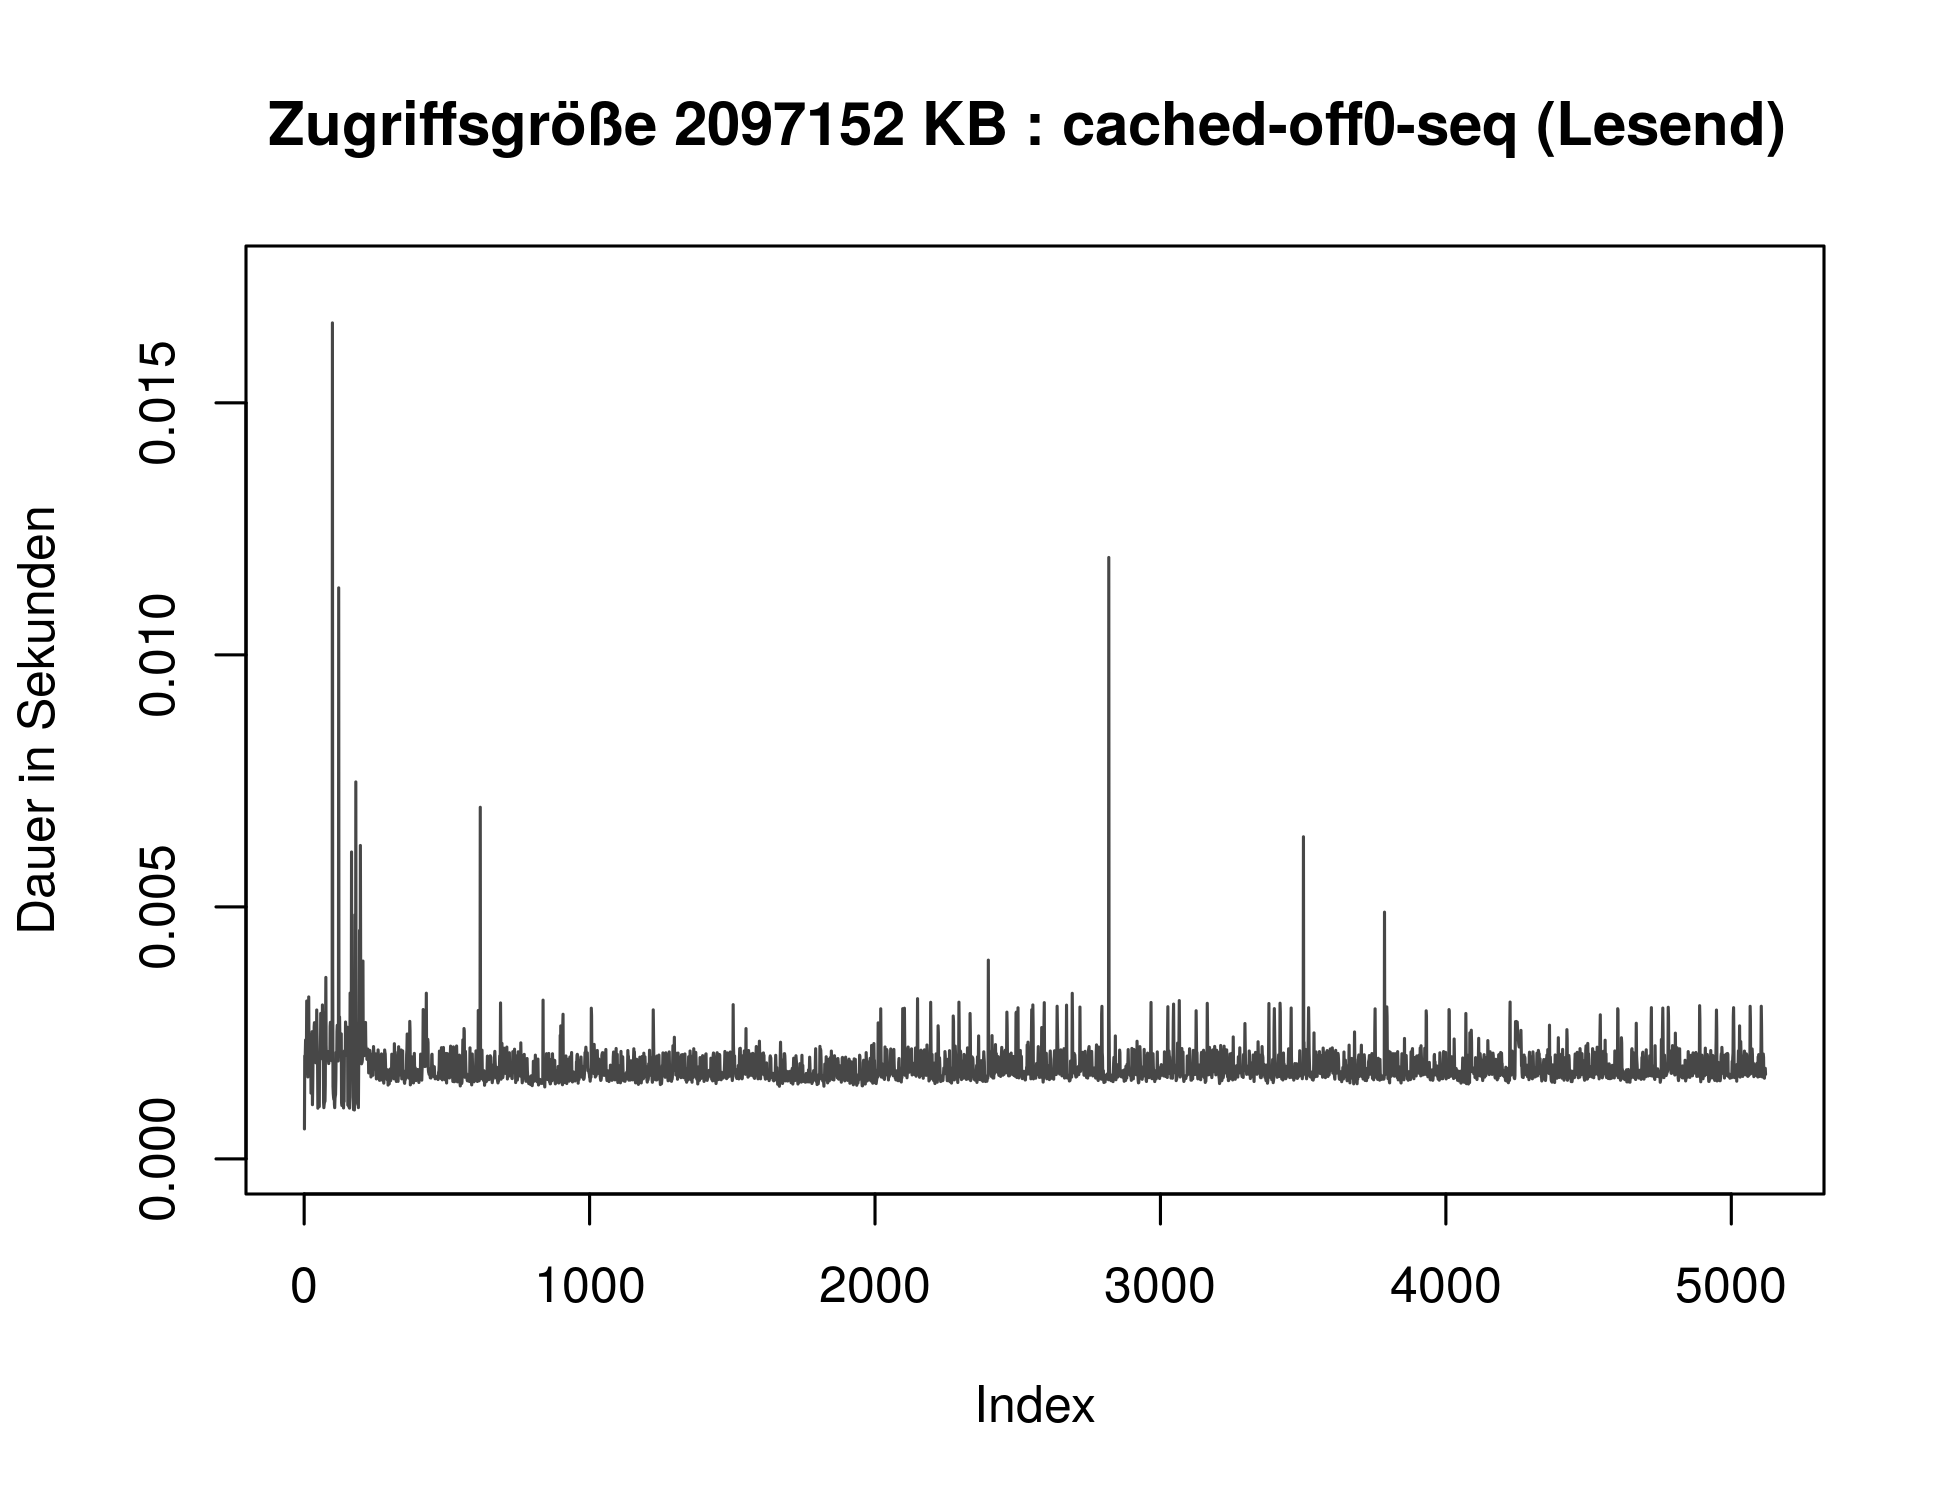
\includegraphics[width=.43\textwidth]{Bilder/Plots/exploration/plot_Size2097152_read_seq.png}
	}
	\hfill
	\subfloat[Messungen mit Zugriffsgröße 2MiB auf SEQ-W]{
		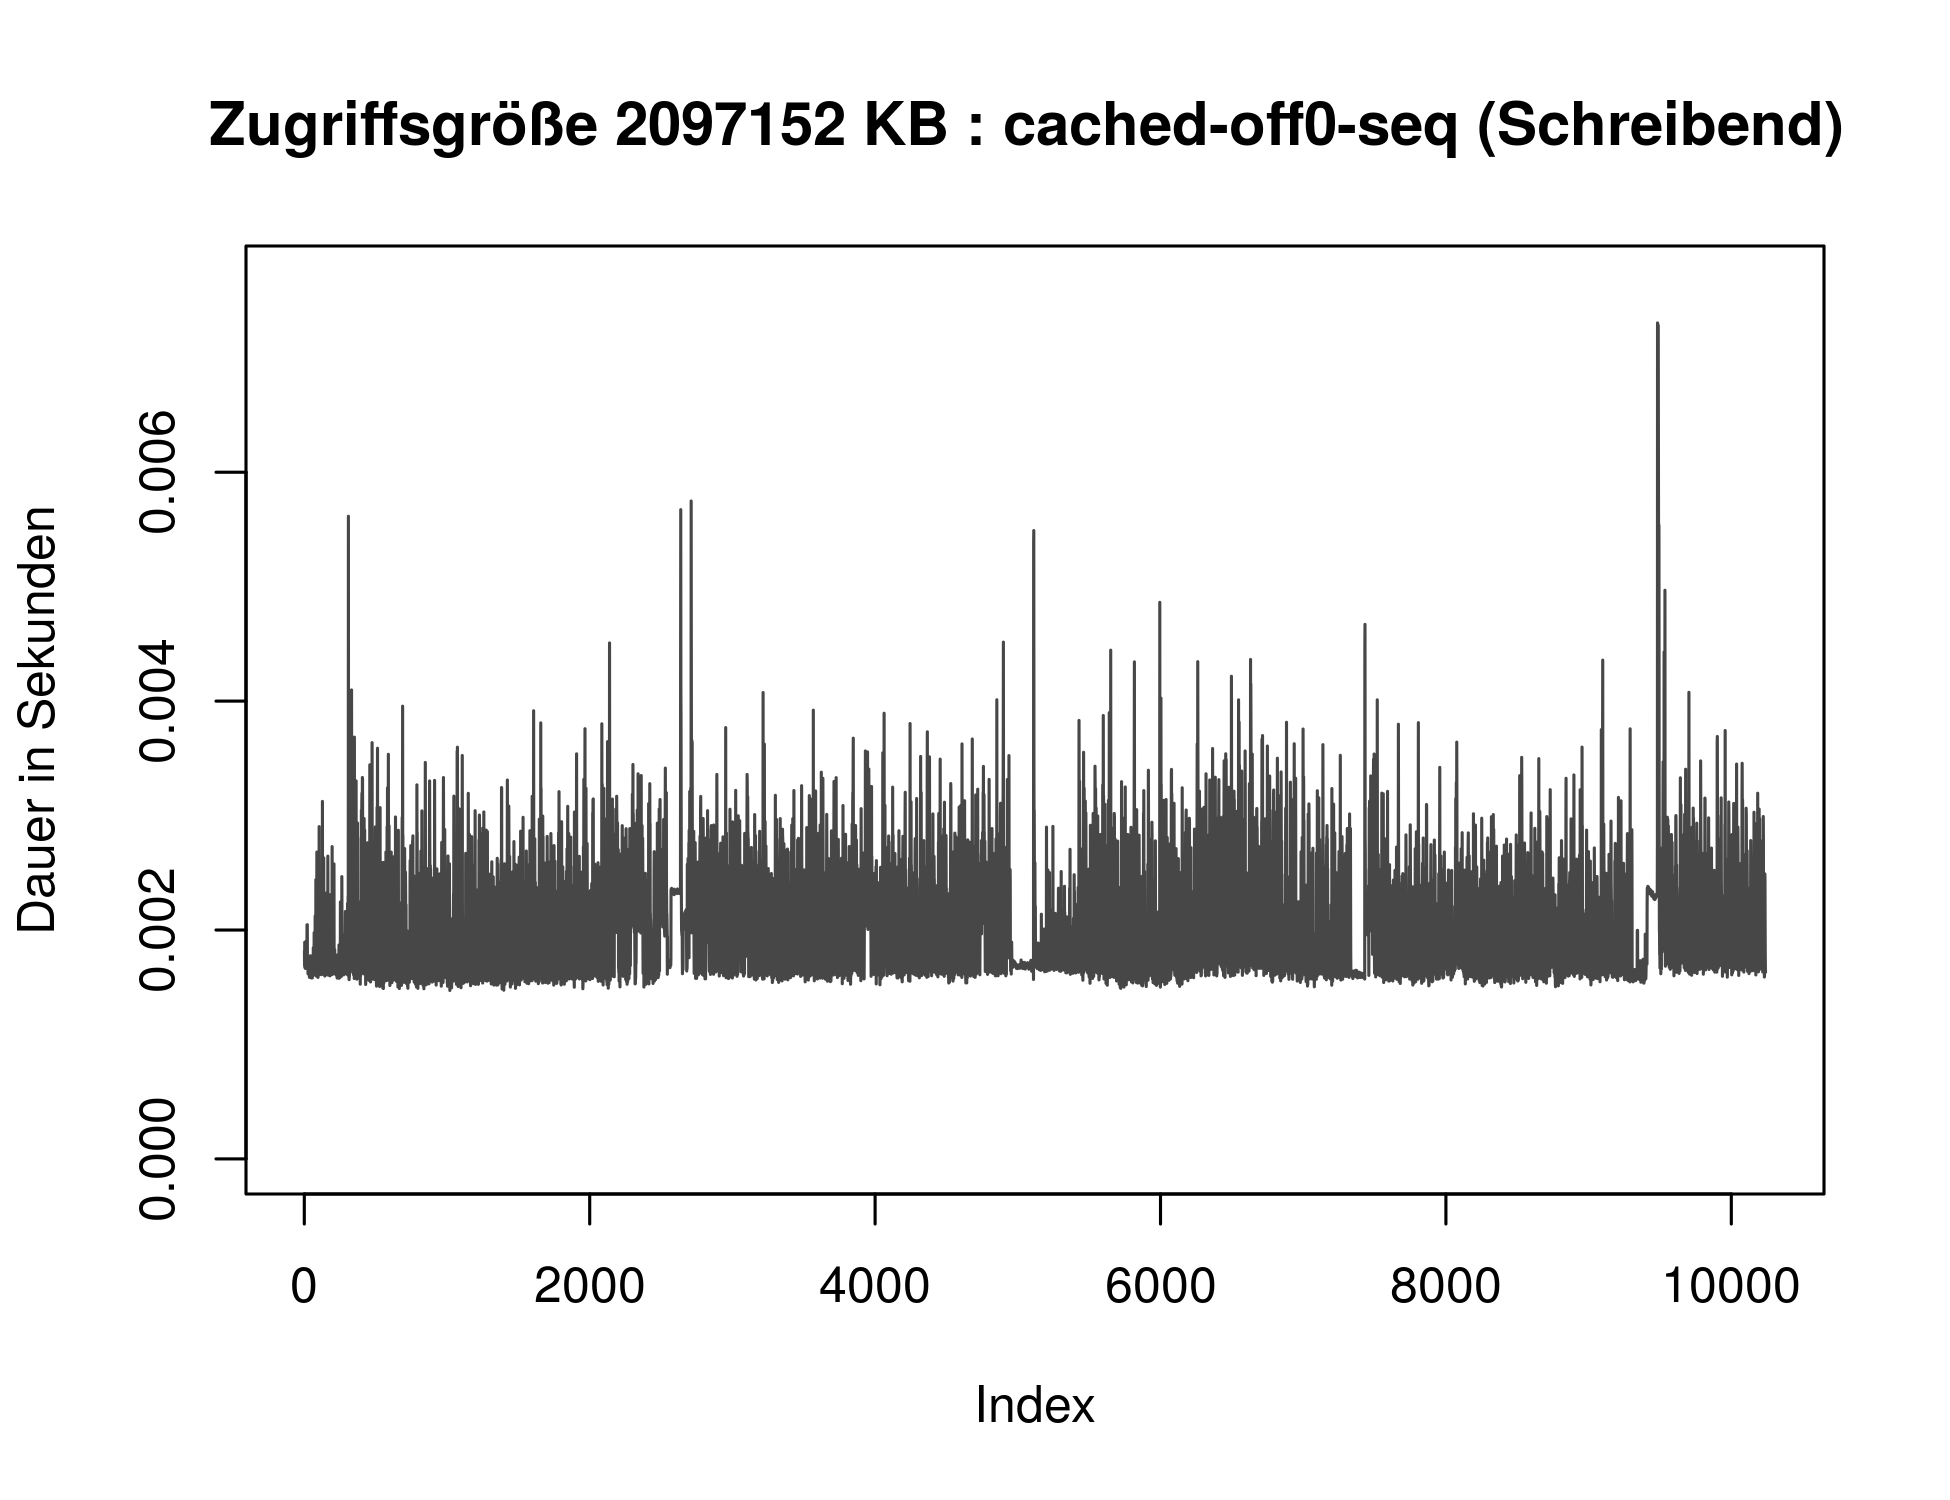
\includegraphics[width=.43\textwidth]{Bilder/Plots/exploration/plot_Size2097152_write_seq.png}
	}\\
	\subfloat[Messungen mit Zugriffsgröße 2MiB auf RND-R]{
		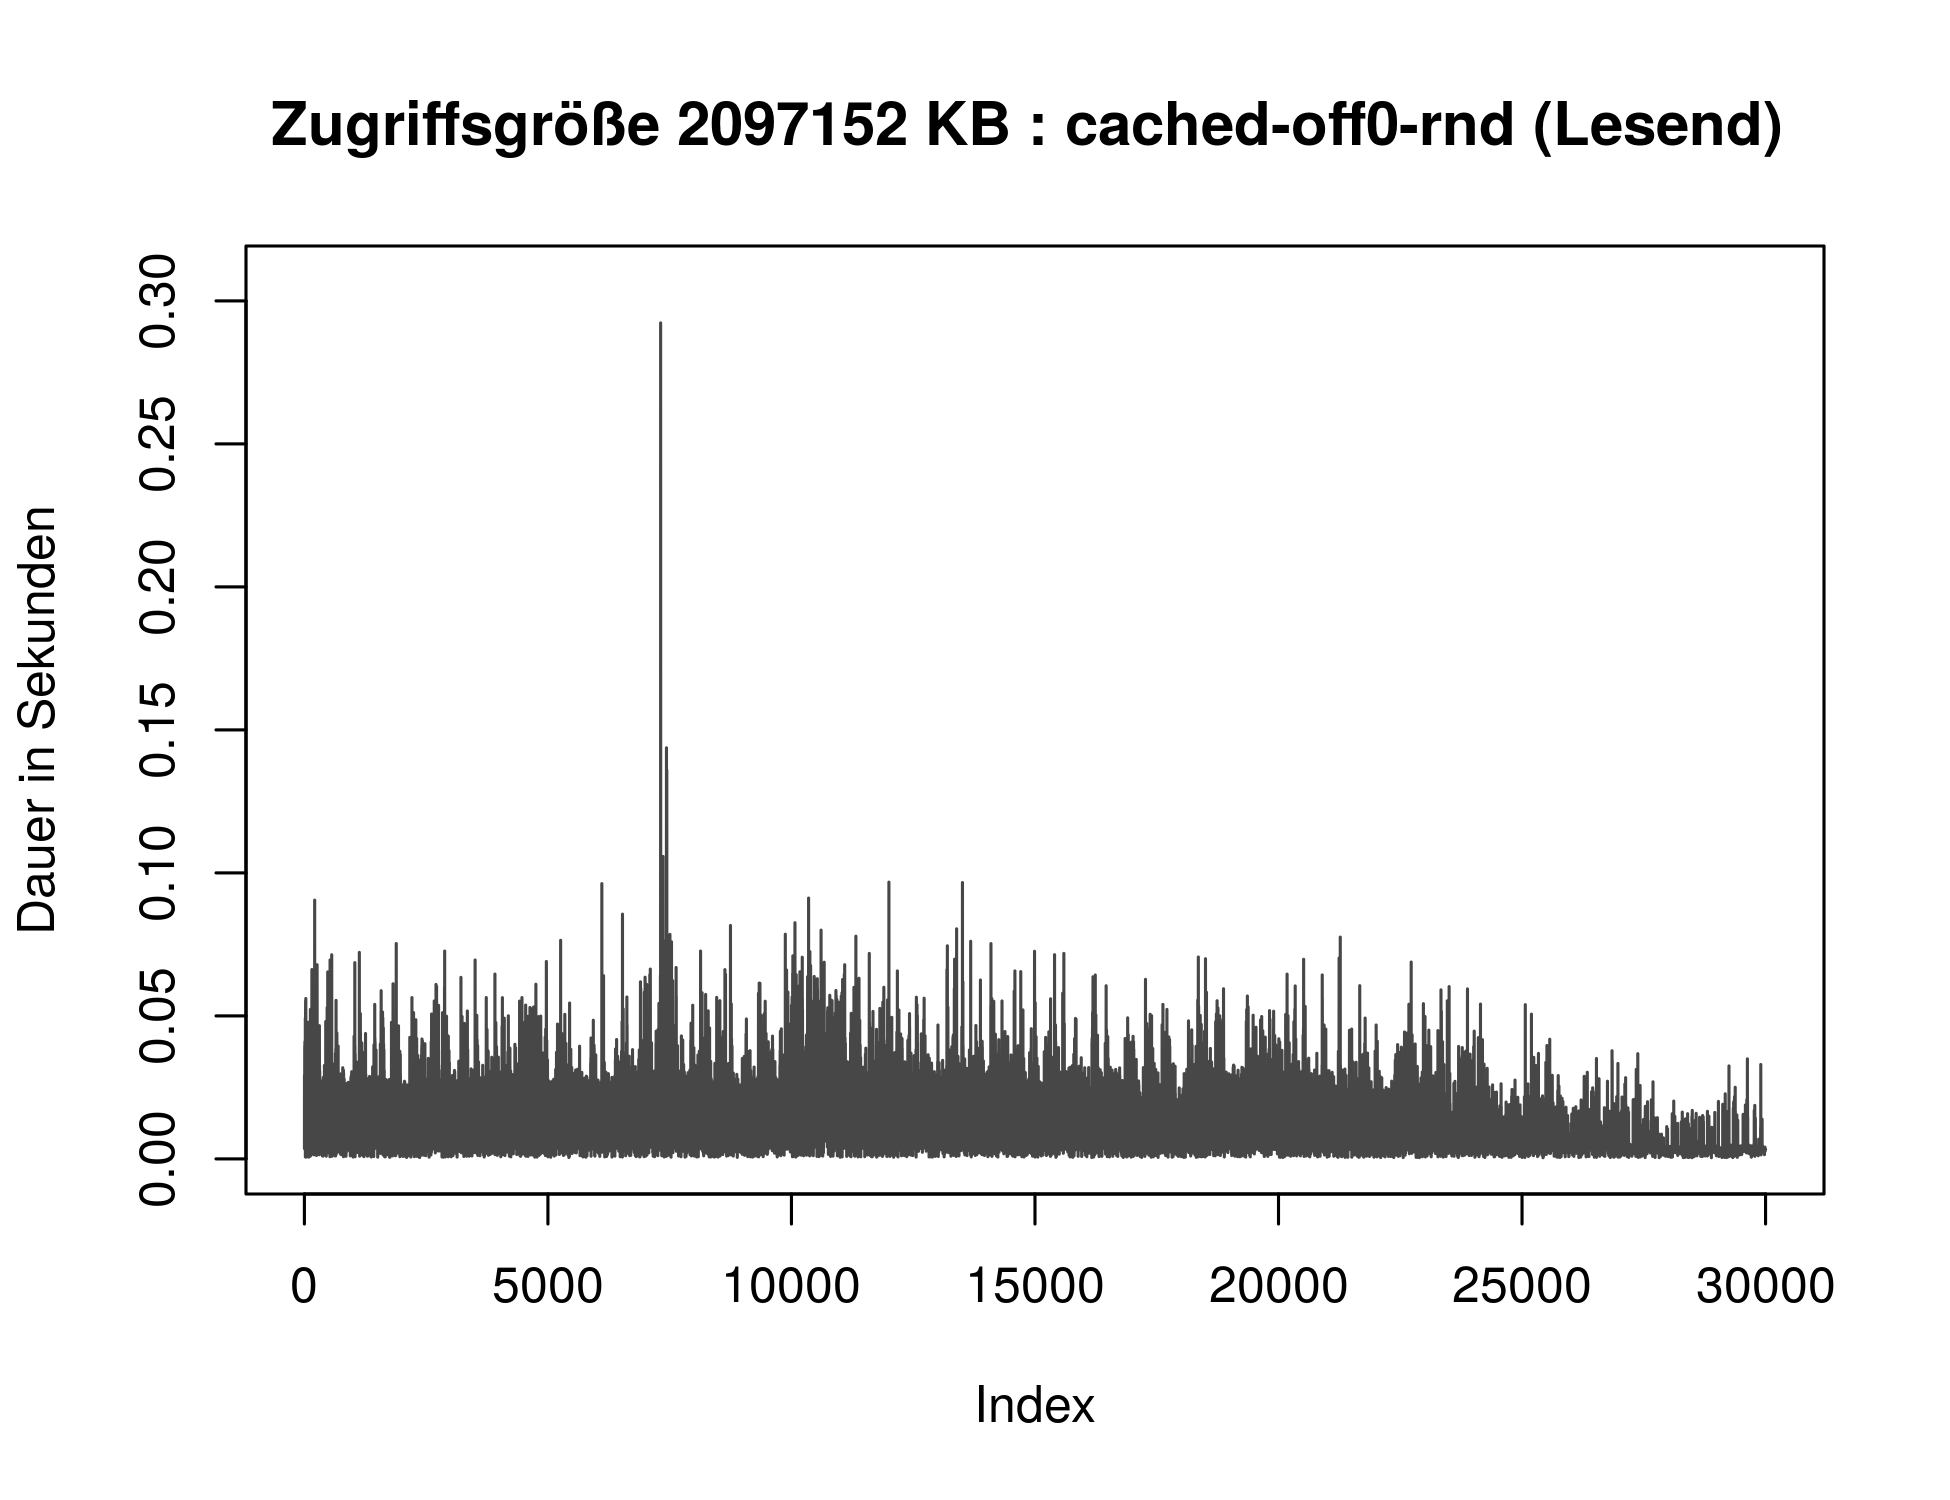
\includegraphics[width=.43\textwidth]{Bilder/Plots/exploration/plot_Size2097152_read_rnd.png}
	}
	\hfill
	\subfloat[Messungen mit Zugriffsgröße 2MiB auf RND-W]{
		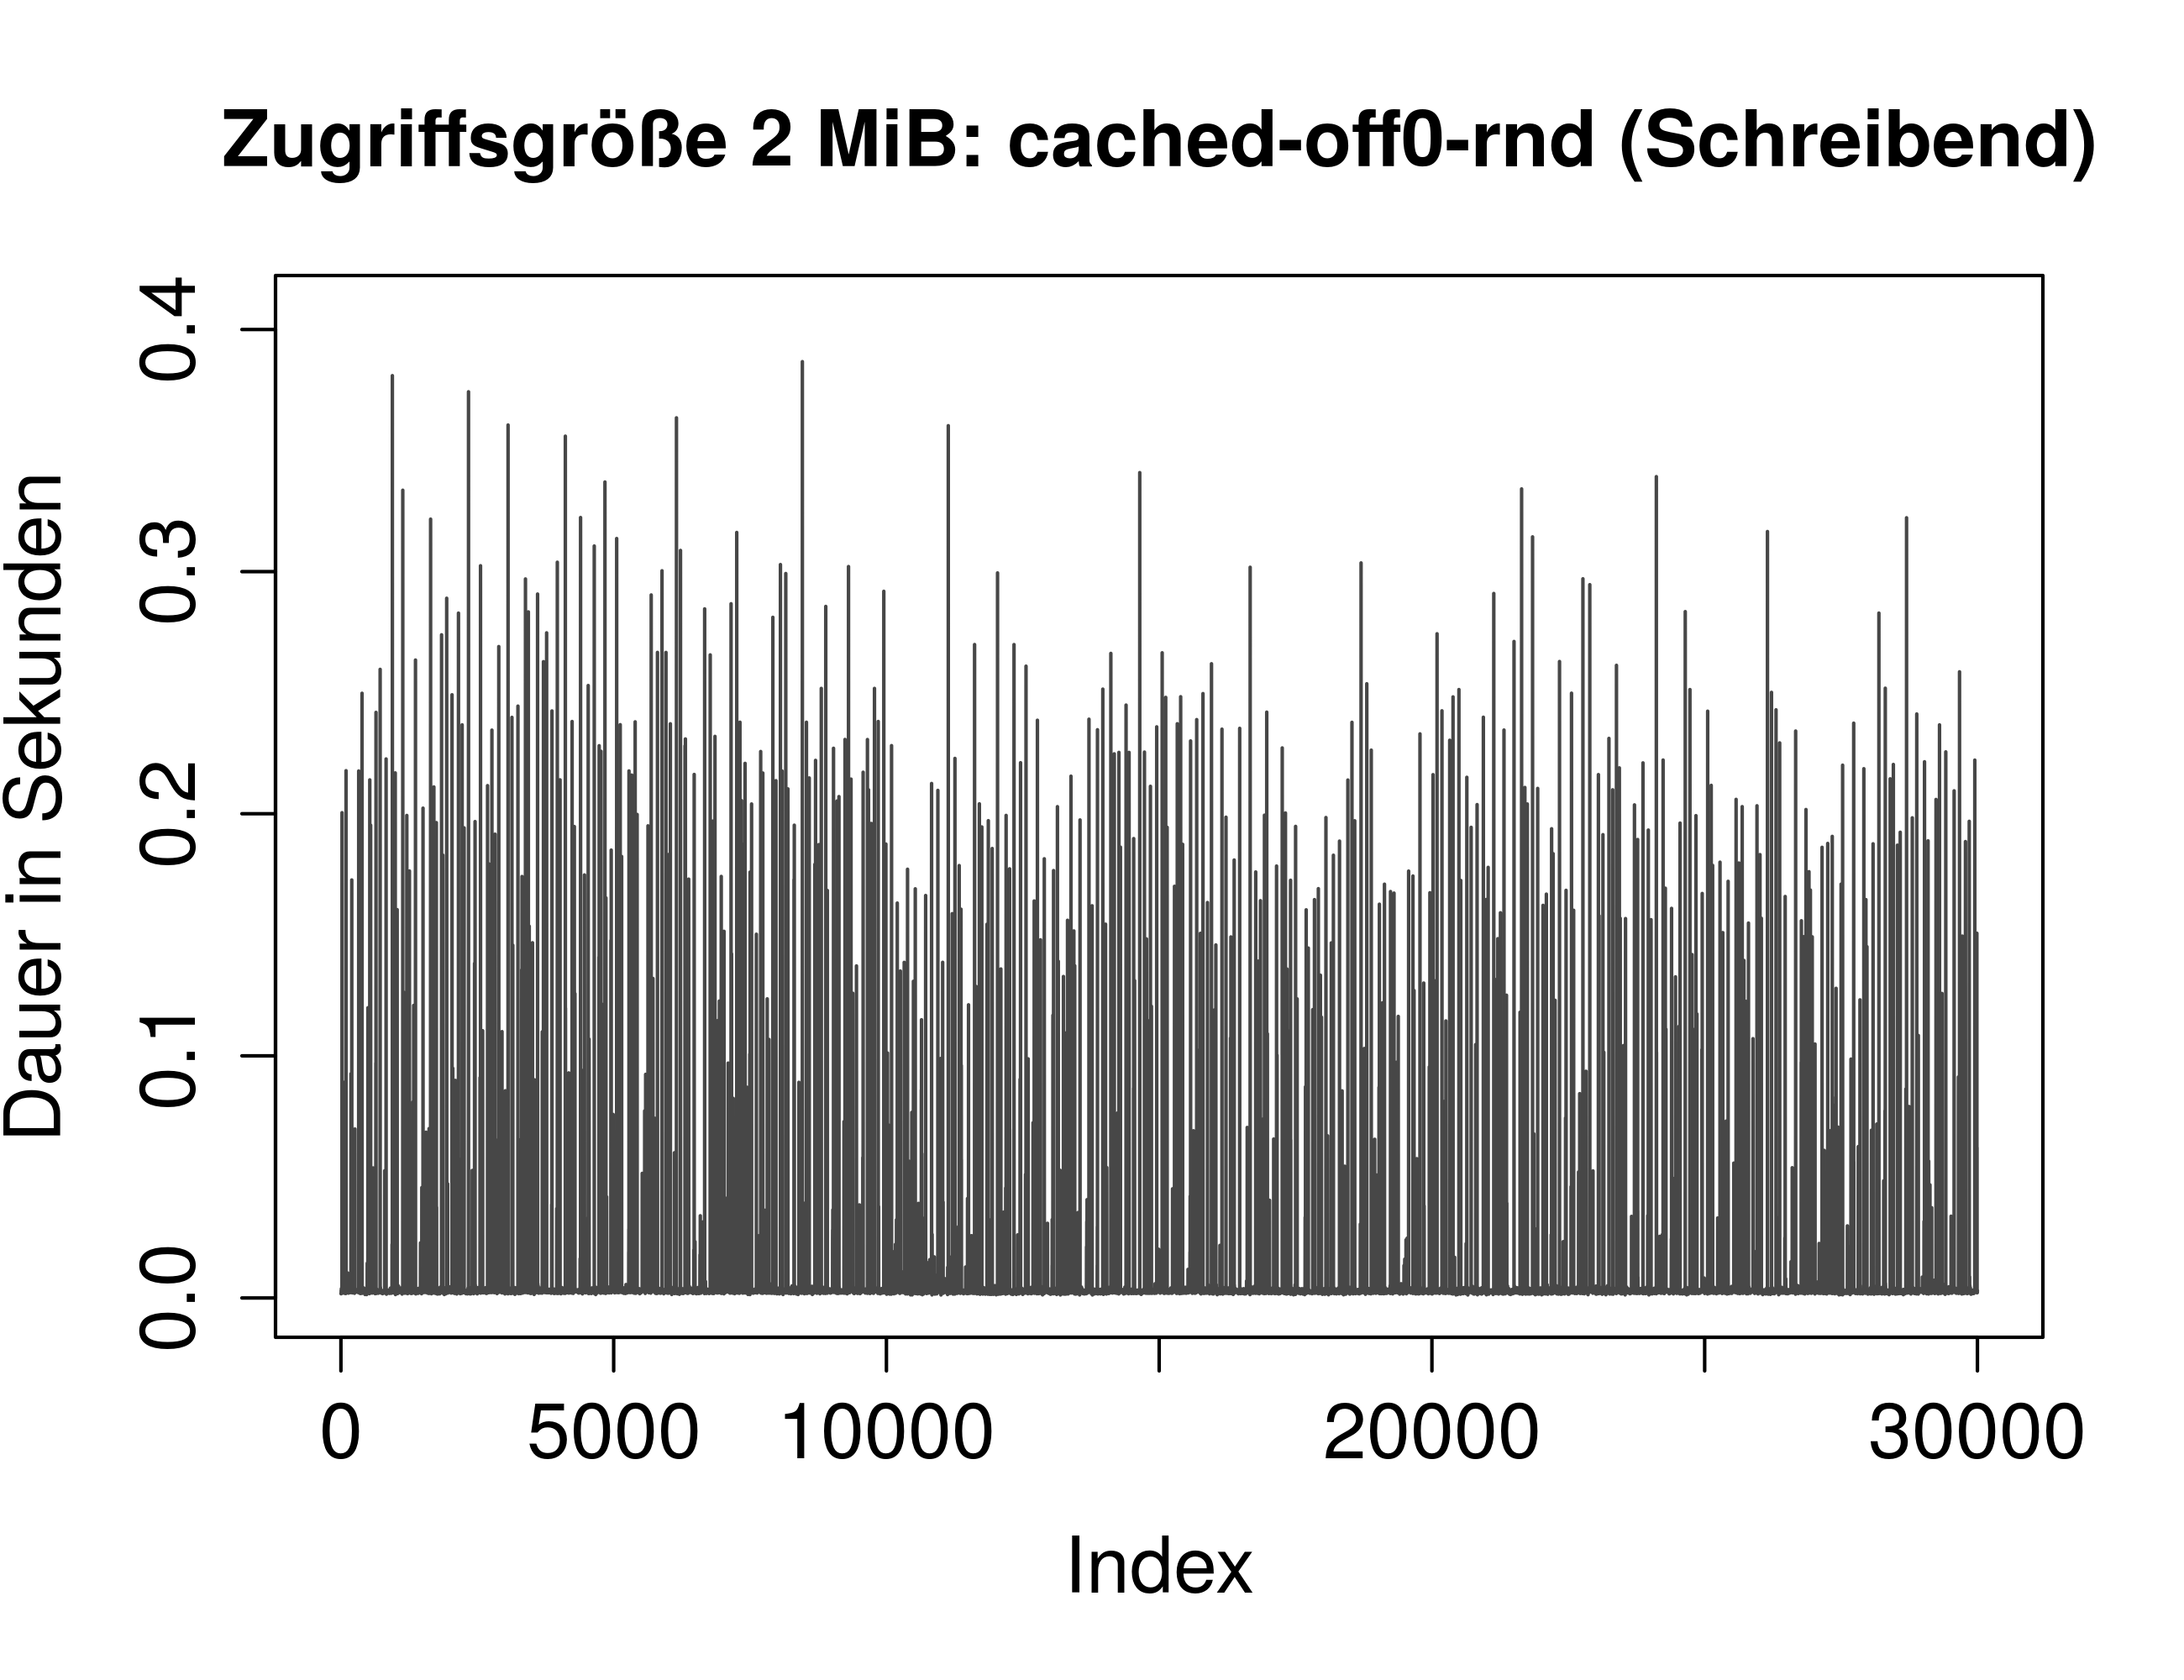
\includegraphics[width=.43\textwidth]{Bilder/Plots/exploration/plot_Size2097152_write_rnd.png}
	}		
	\vspace*{-0.3cm}
	\caption{Detailbetrachtung aller Messungen mit Zugriffsgröße 2MiB}
	\label{fig:groesse2097152}
\end{figure}
\clearpage
\subsubsection{Ausschnittweise Betrachtung der Messungen}
Um die Messdaten zur Untersuchung noch detaillierter darzustellen, müssen kleine Ausschnitte herausgegriffen werden. Zunächst betrachte ich die ersten $250$ Messungen jedes Experiments.
In der Abbildung \ref{fig:first250}b zum Datensatz SEQ-W eine gewisse Periodizität der Zugriffszeiten vorhanden zu sein. Etwa alle 45 Messungen gibt es einen größeren Sprung, alternierend sind die Laufzeiten jeweils etwas langsamer und schneller.
Nach genau $123$ Punkten scheint sich das Muster zu wiederholen, dort befindet sich der zweitgrößte Messwert der Laufzeit in diesem Ausschnitt.\\
Ein erstes simples Modell könnte es nun sein, eine Fortführung der augenscheinlichen Periodizität anzuwenden, indem die ersten $123$ Zugriffszeiten für die Laufzeiten 123 bis 246 vorhergesagt werden.
Wenn man diese Vorhersagen jedoch über die tatsächlichen Zugriffszeiten legt (siehe Abbildung \ref{fig:periodicity}), so erkannt man doch, dass der Verlauf der Messungen von dieser Periode abweicht.\\ 
Bei den anderen Graphen kann keine so simple Periodizität beobachtet werden.
In den Graphen \ref{fig:first250}a und \ref{fig:first250}c sind besonders starke Ausreißer nach oben in den Laufzeiten zu erkennen. In Abbildung \ref{fig:first250}d sind dagegen einige Ausreißer, die wesentlich schneller bearbeitet wurden.\\
Einzelne sehr starke Ausreißer, wie bei SEQ-R, sind vermutlich durch außergewöhnlich große queue-Zeiten entstanden, regelmäßigere Ausreißer sind ein Zeichen für systematisch anders behandelte E/A-Zugriffe, die sich vielleicht durch verschiedene E/A-Pfade unterscheiden.

\begin{figure}
	\subfloat[Die ersten 250 Messungen in SEQ-R]{
		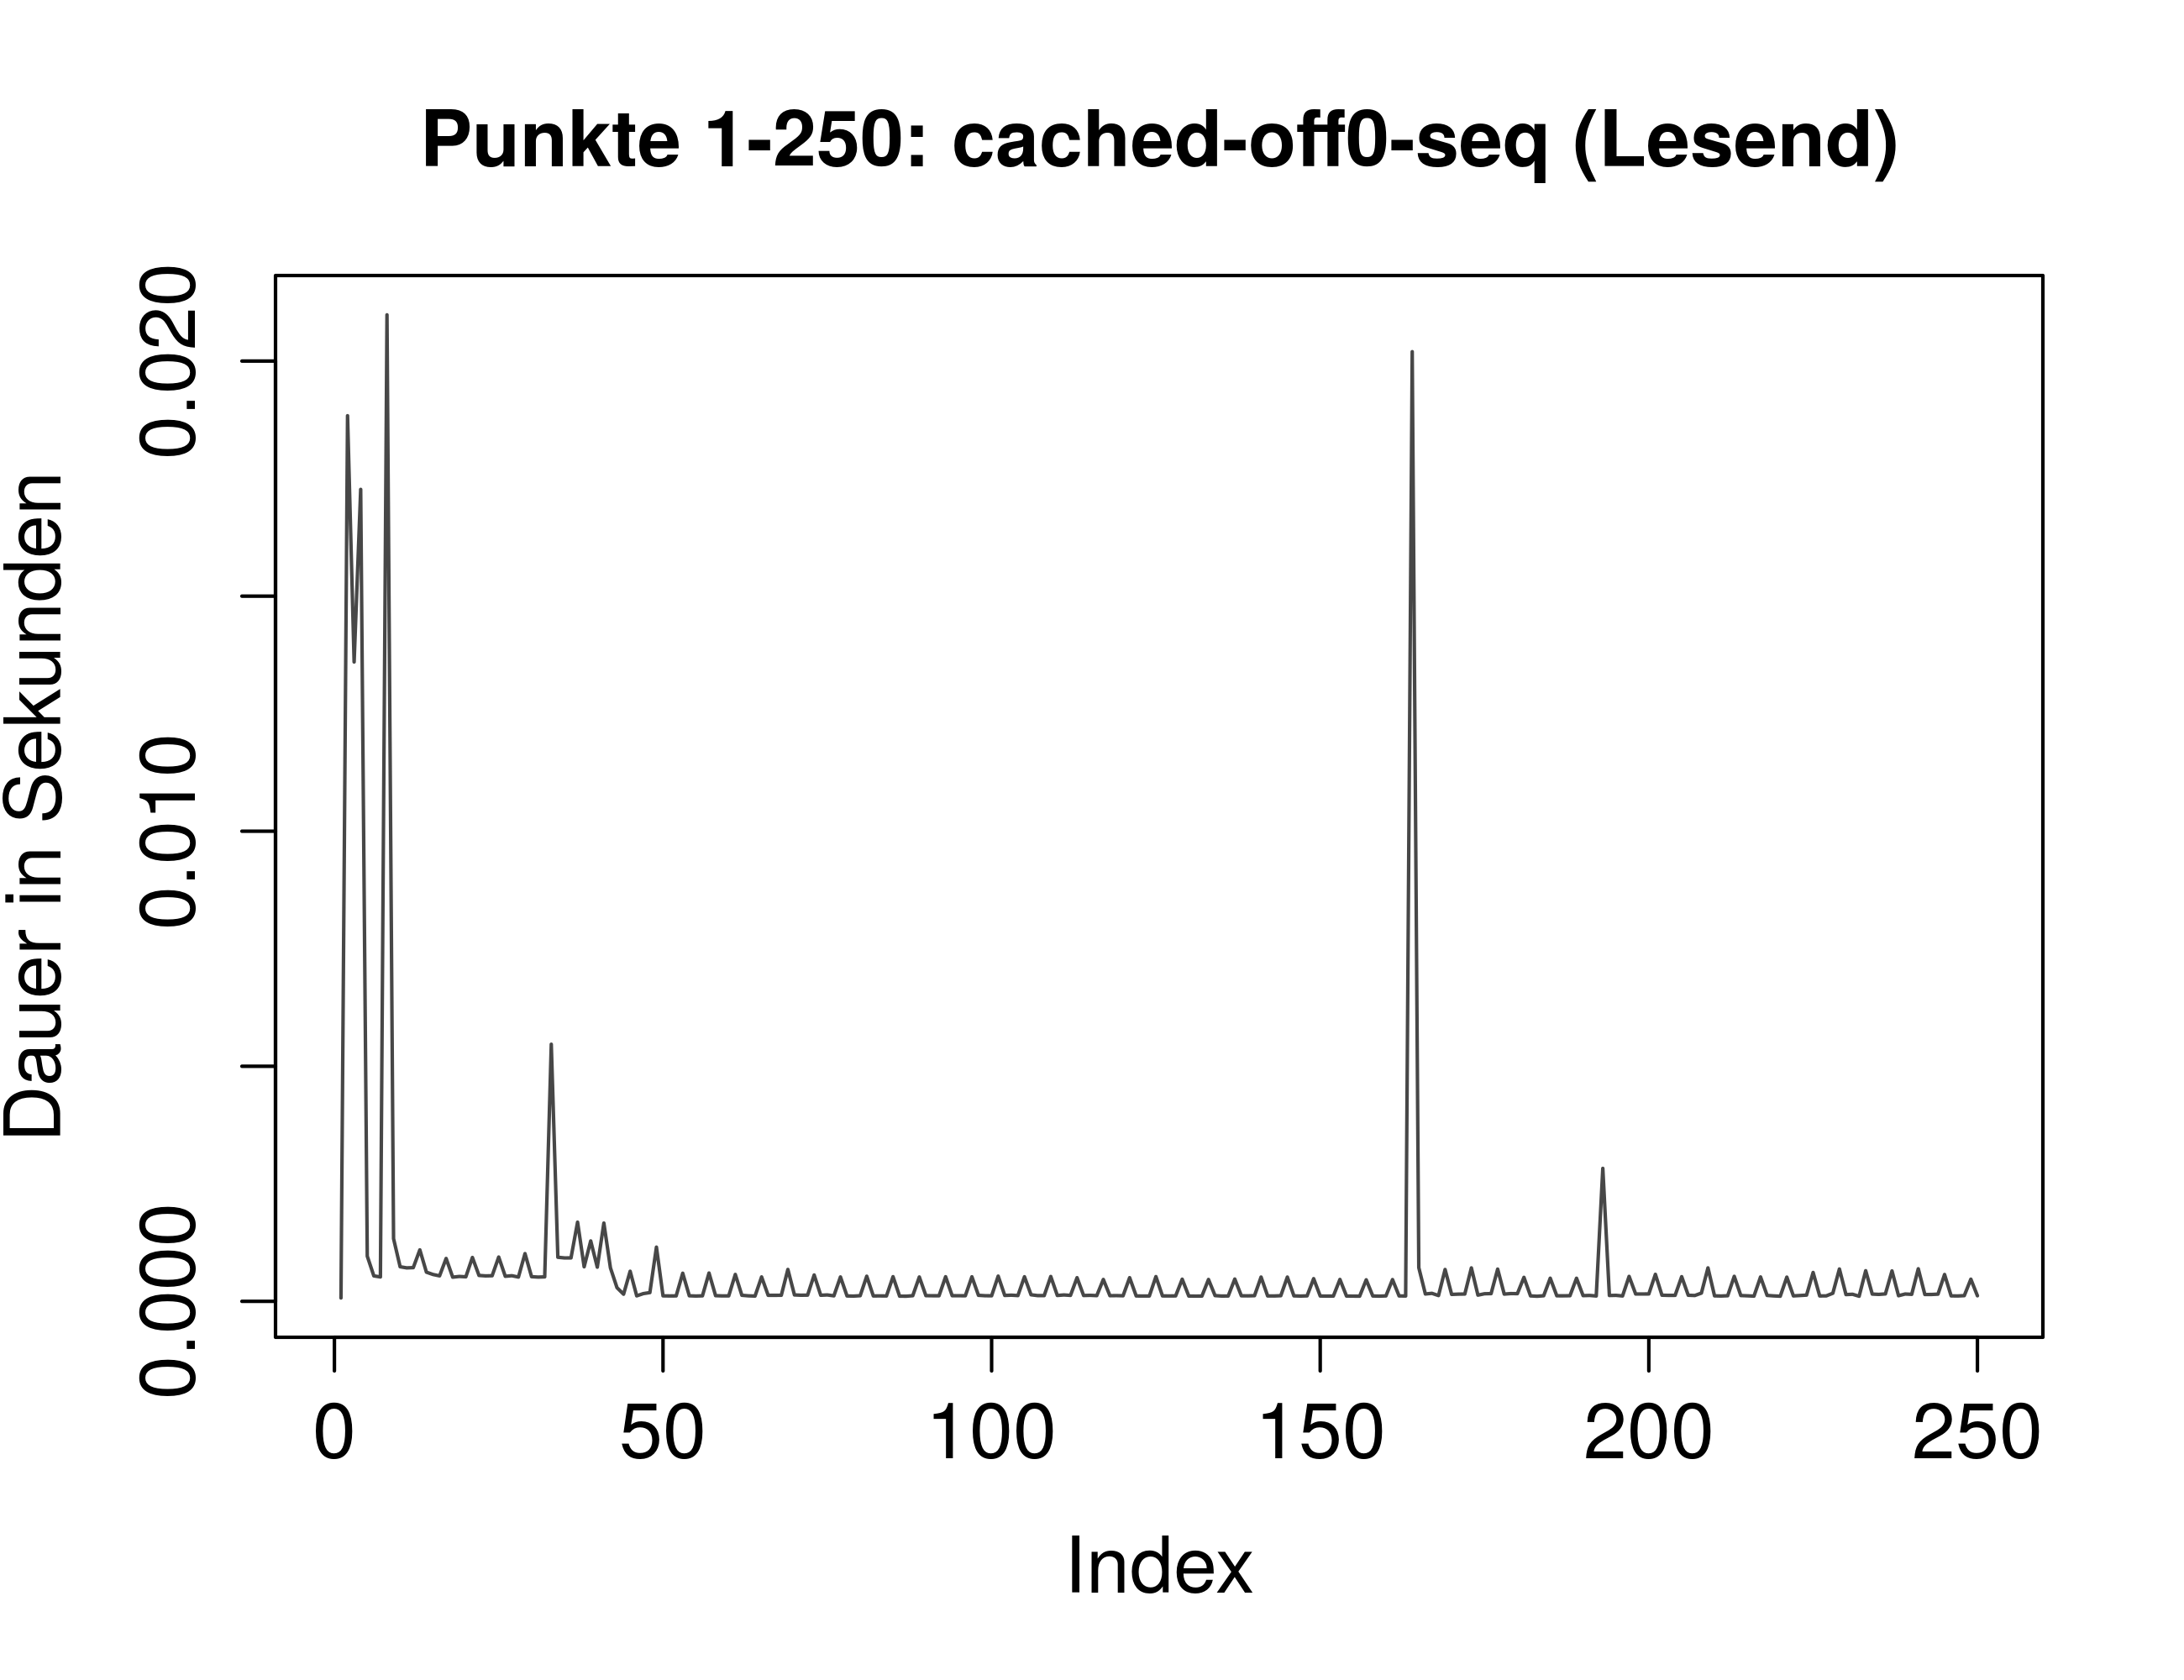
\includegraphics[width=.43\textwidth]{Bilder/Plots/exploration/plot_First250_read_seq.png}
	}
	\hfill
	\subfloat[Die ersten 250 Messungen in SEQ-W]{
		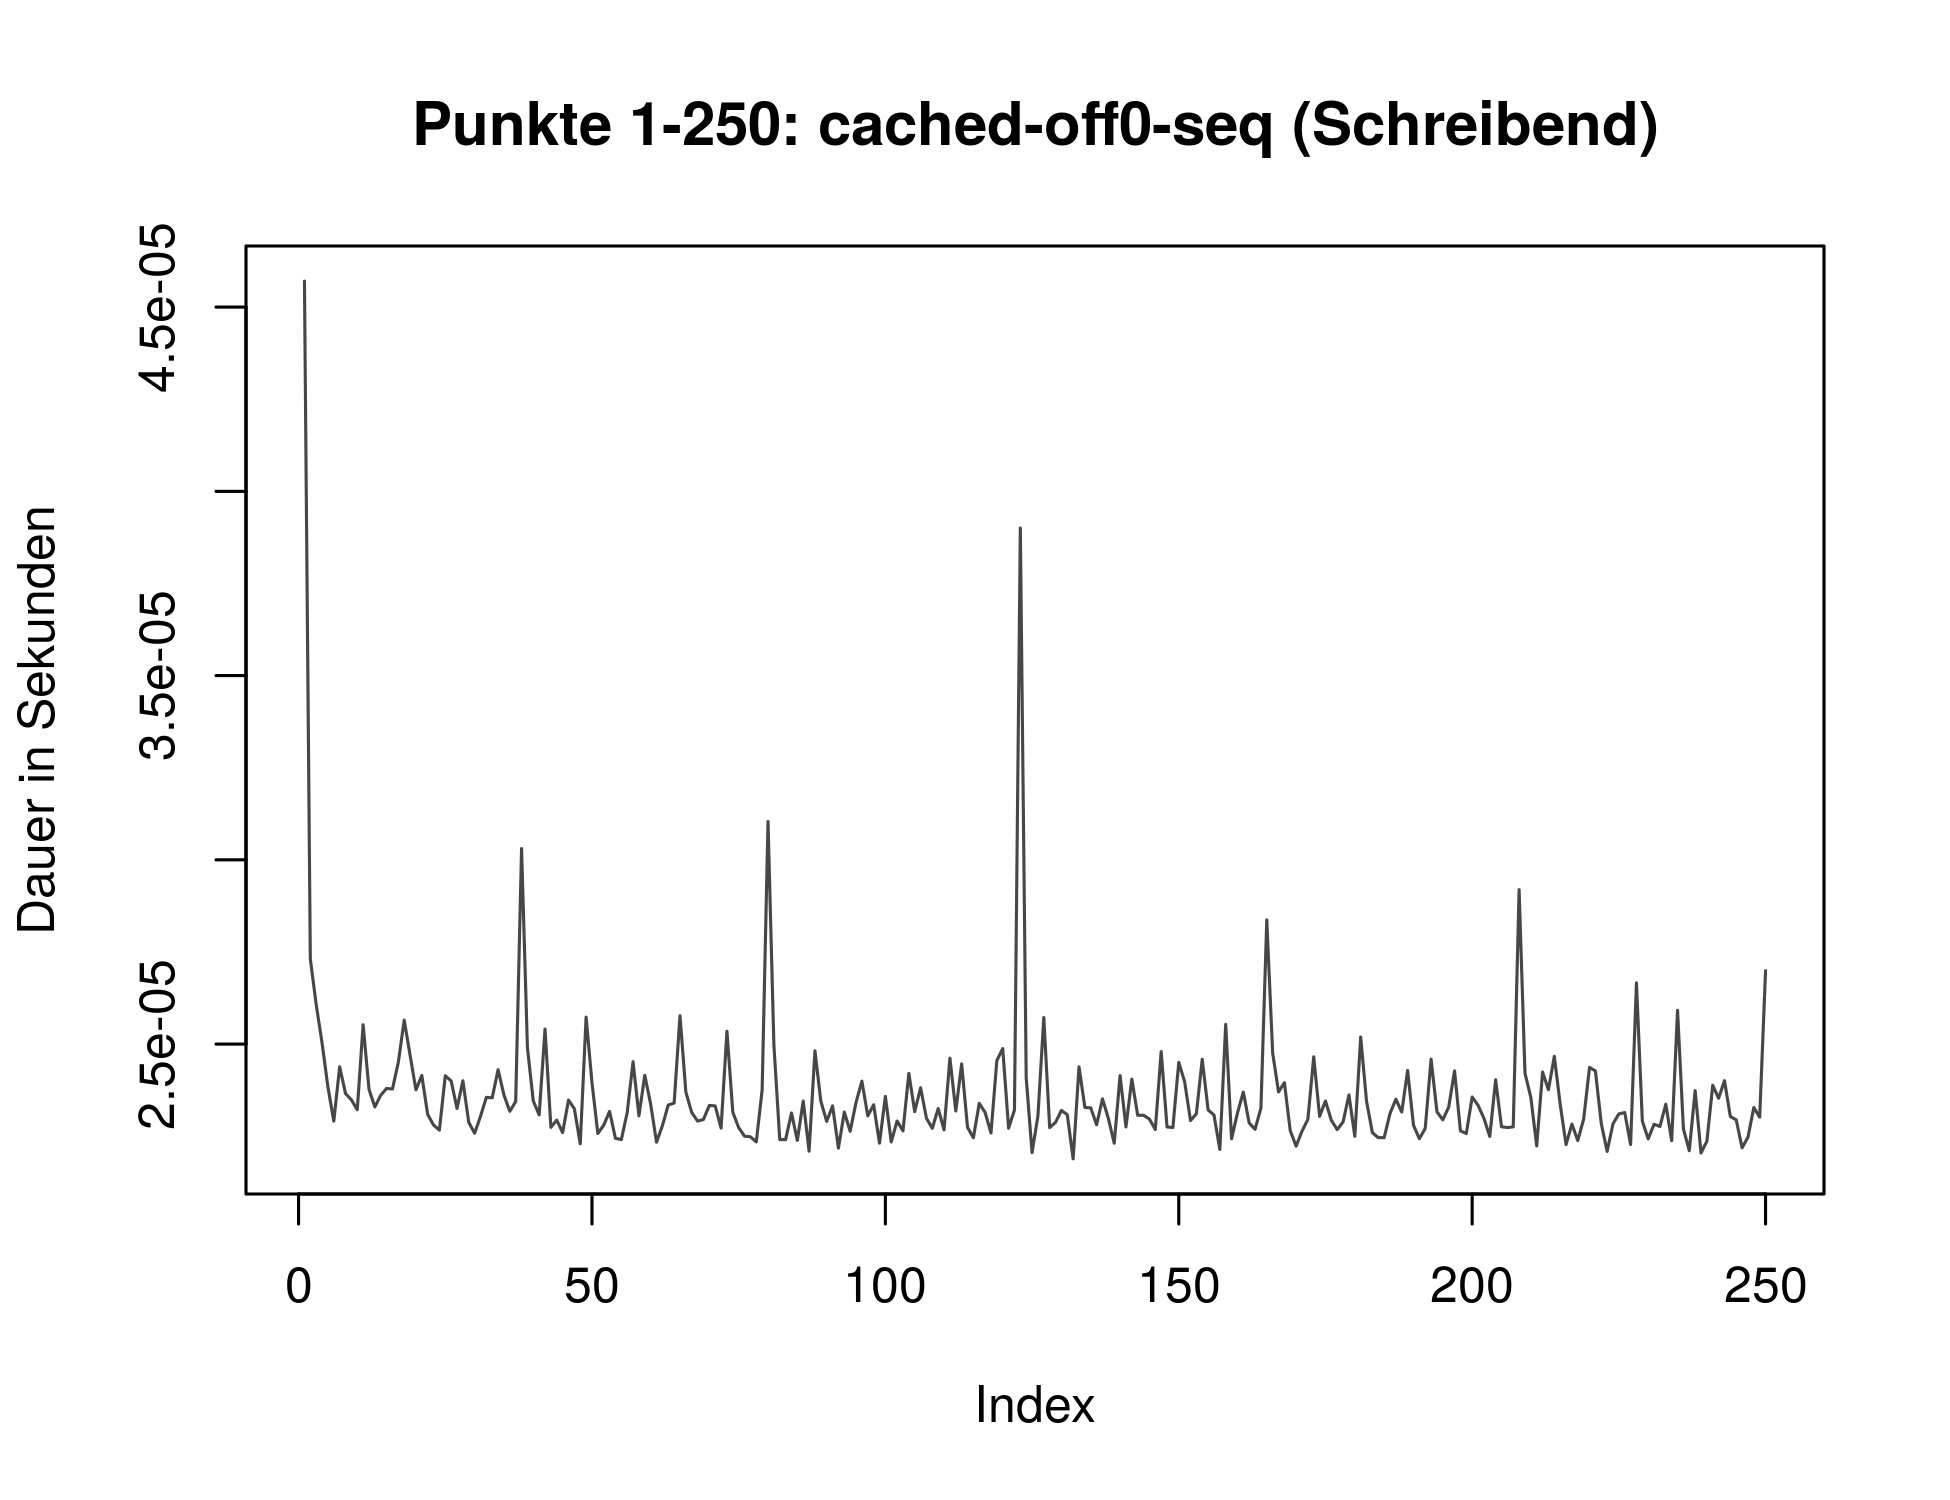
\includegraphics[width=.43\textwidth]{Bilder/Plots/exploration/plot_First250_write_seq.png}
	}\\
	\subfloat[Die ersten 250 Messungen in RND-R]{
		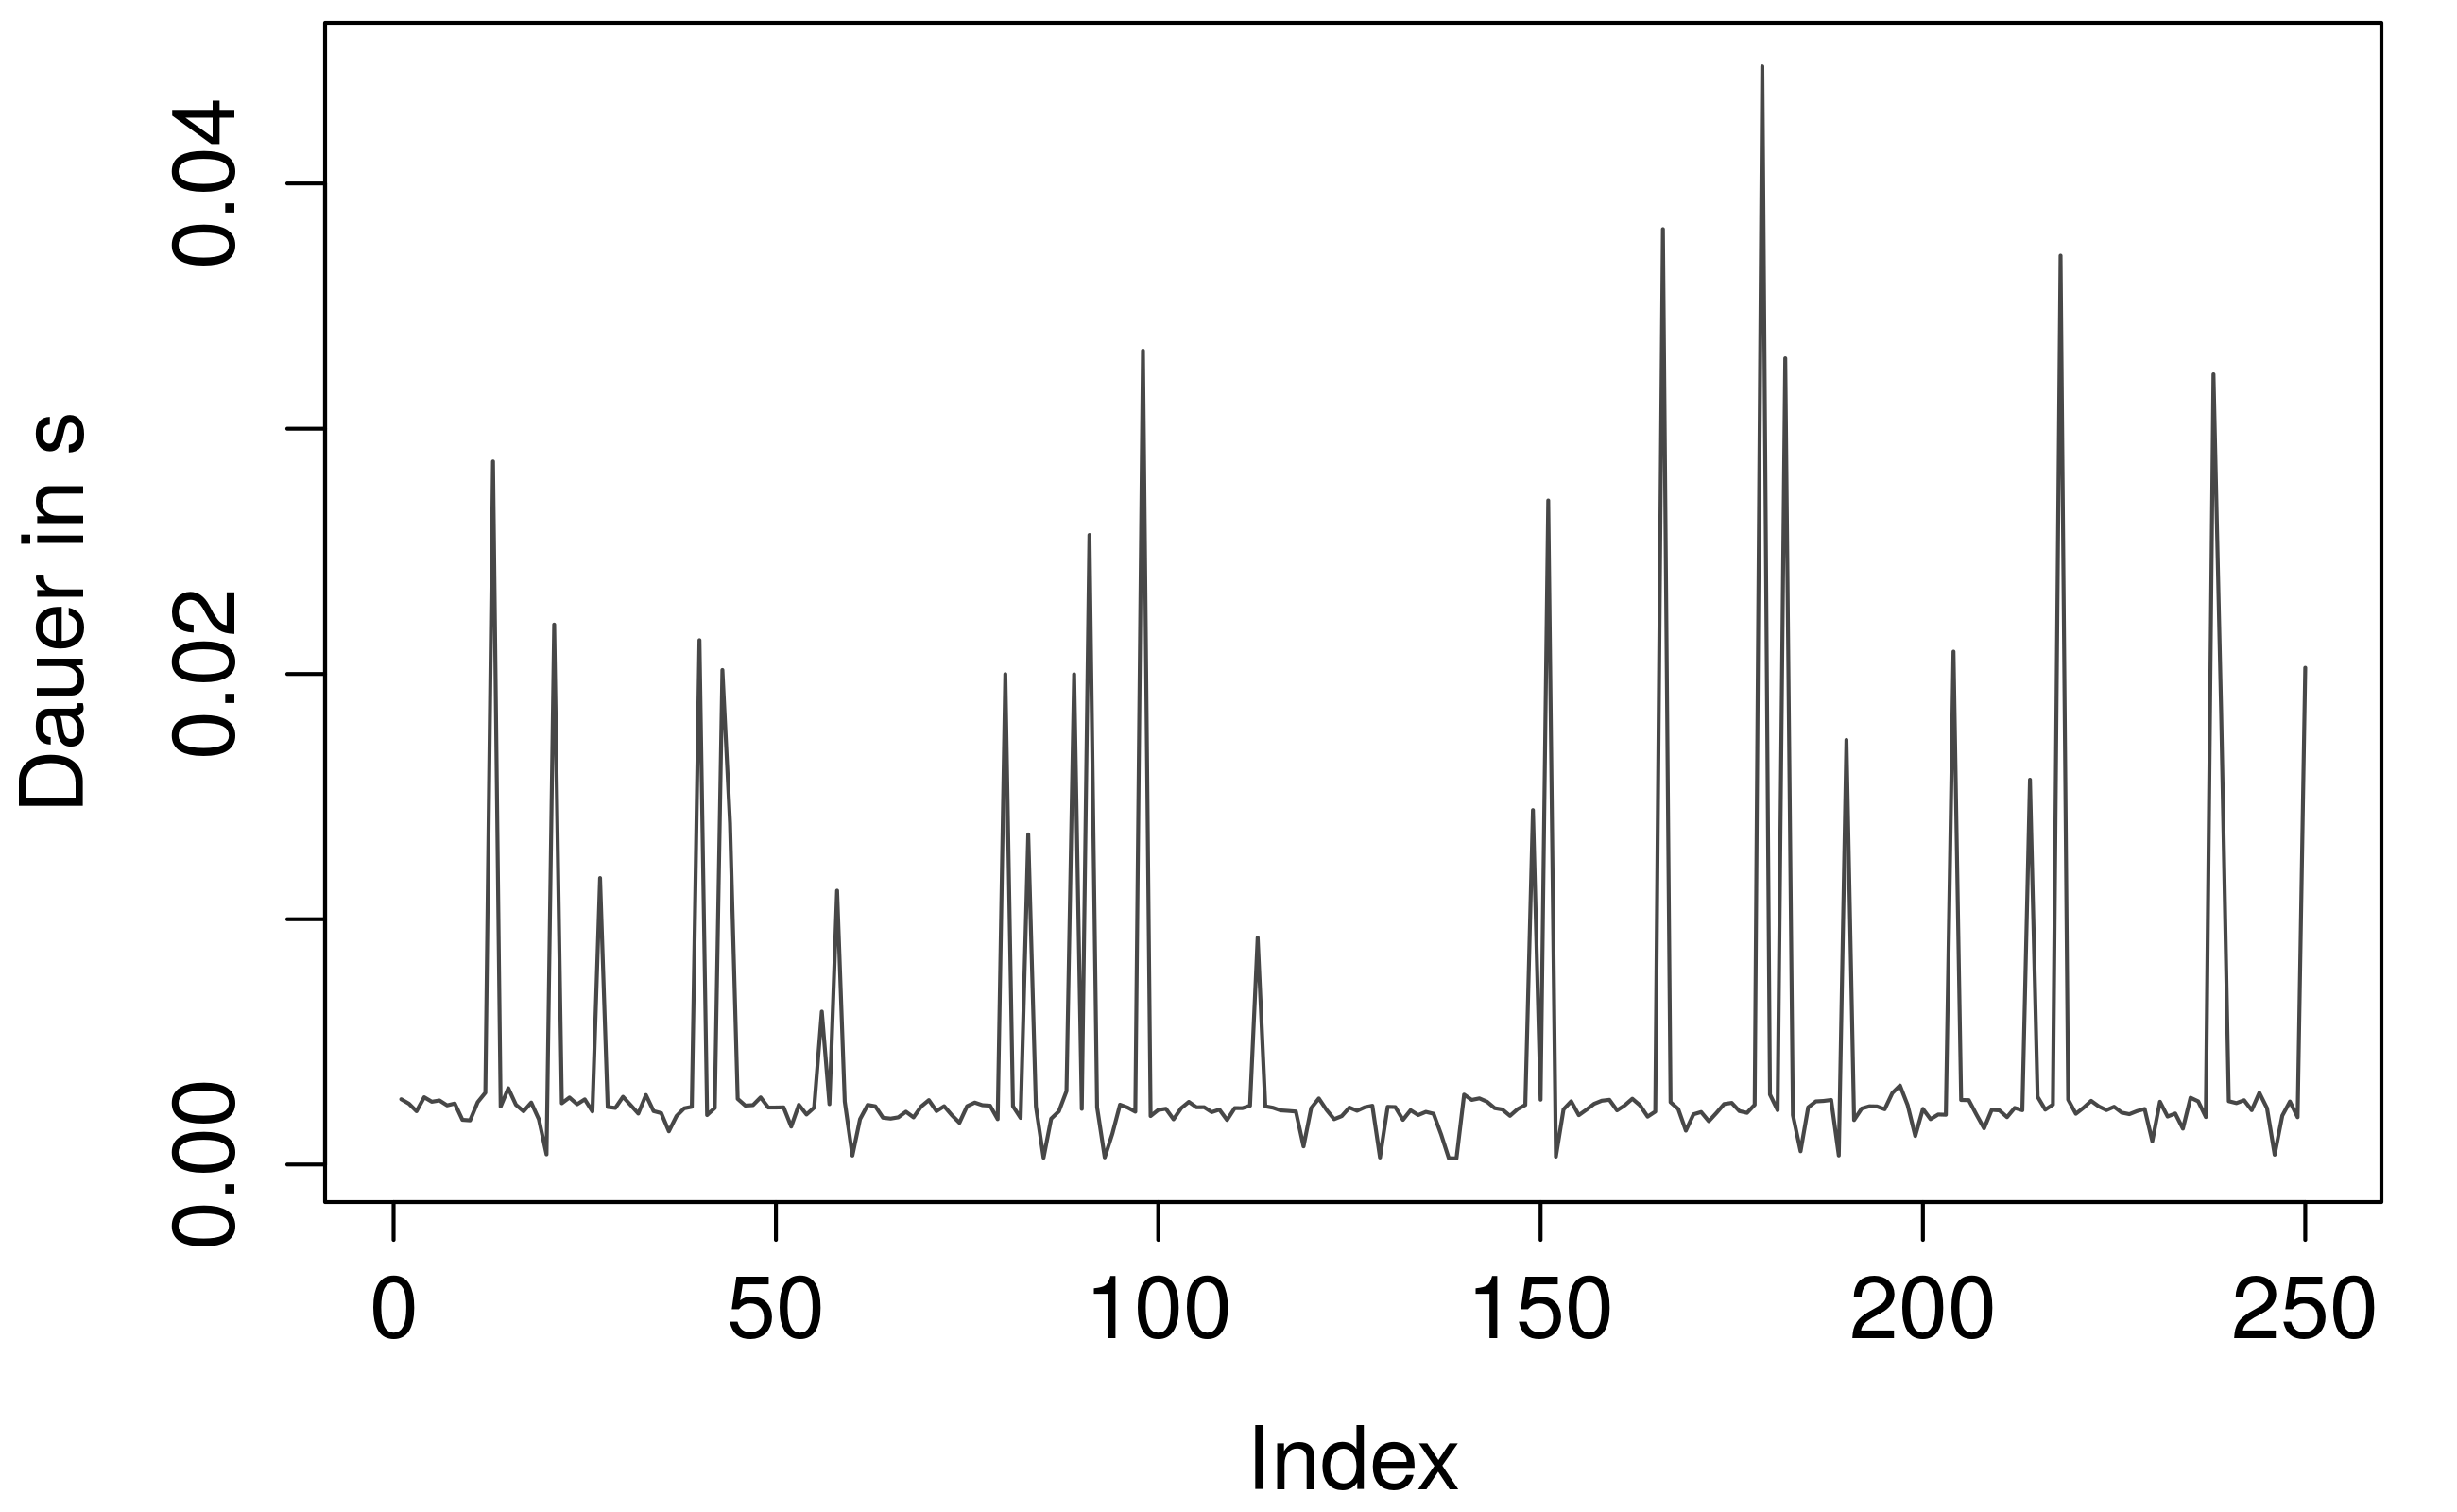
\includegraphics[width=.43\textwidth]{Bilder/Plots/exploration/plot_First250_read_rnd.png}
	}
	\hfill
	\subfloat[Die ersten 250 Messungen in RND-W]{
		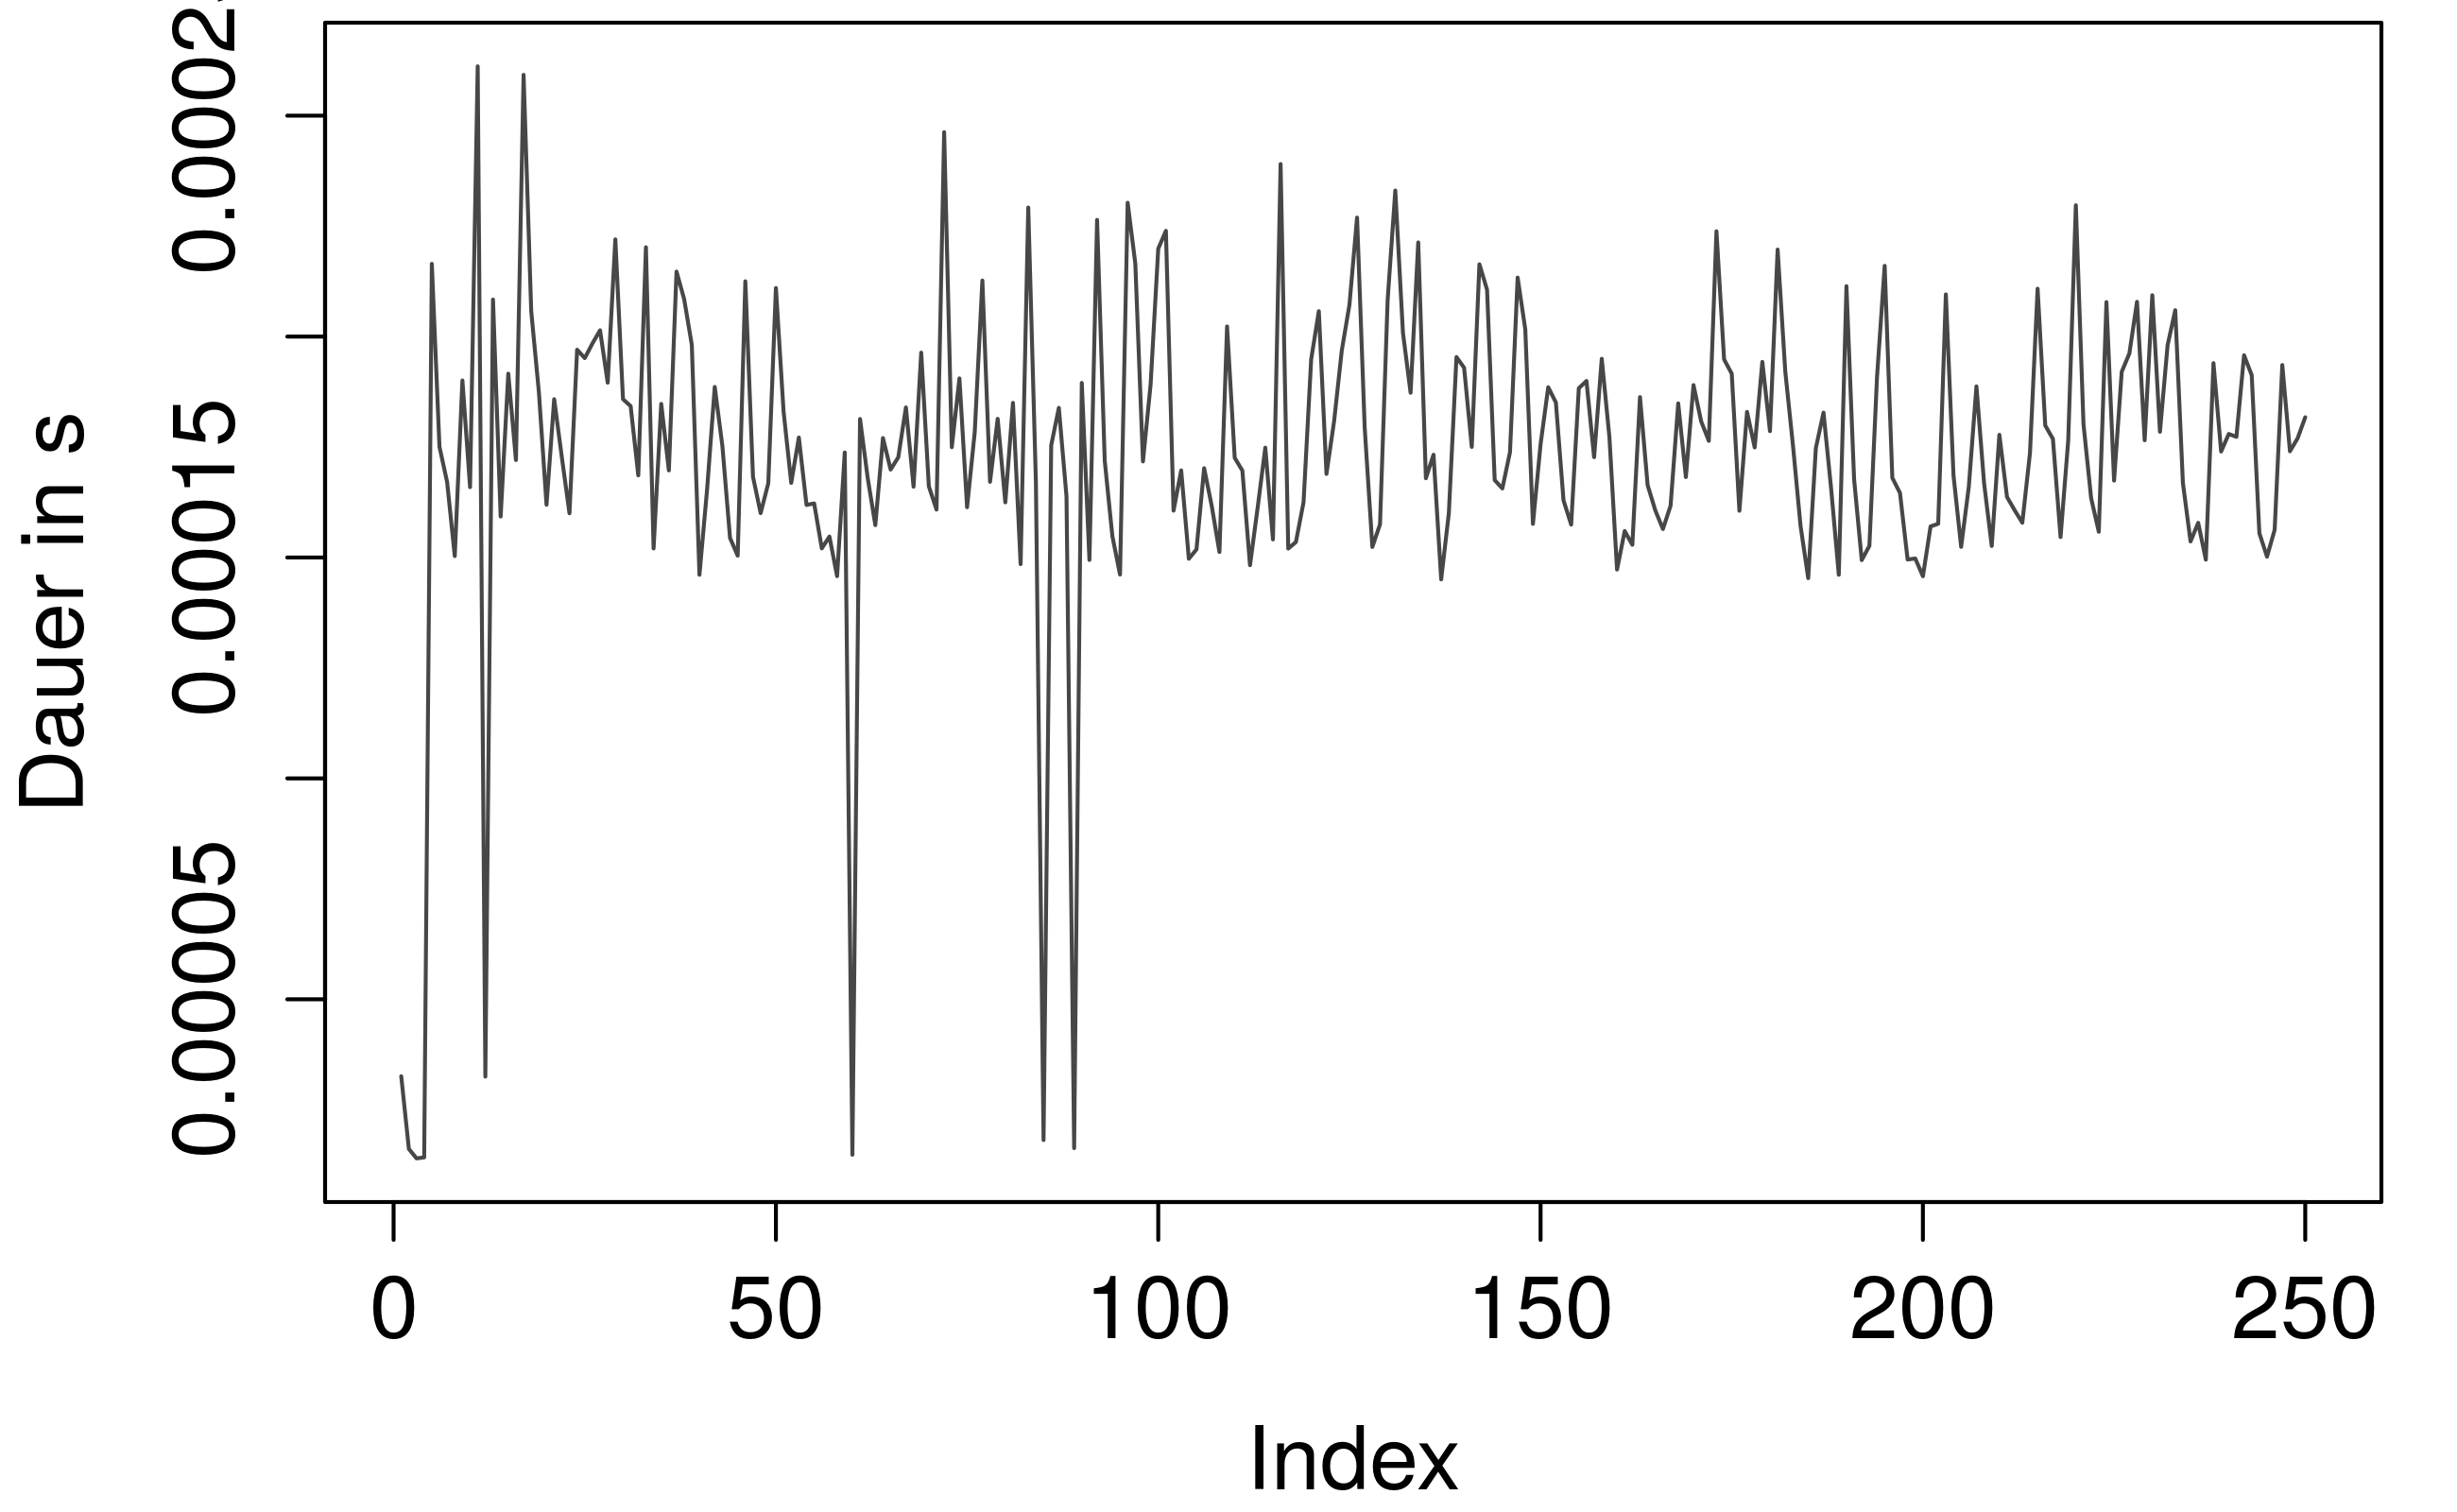
\includegraphics[width=.43\textwidth]{Bilder/Plots/exploration/plot_First250_write_rnd.png}
	}		
	\caption{Detailbetrachtung der ersten 250 Messungen}
	\label{fig:first250}
\end{figure} 

\begin{figure}
	\begin{center}
		\subfloat{
			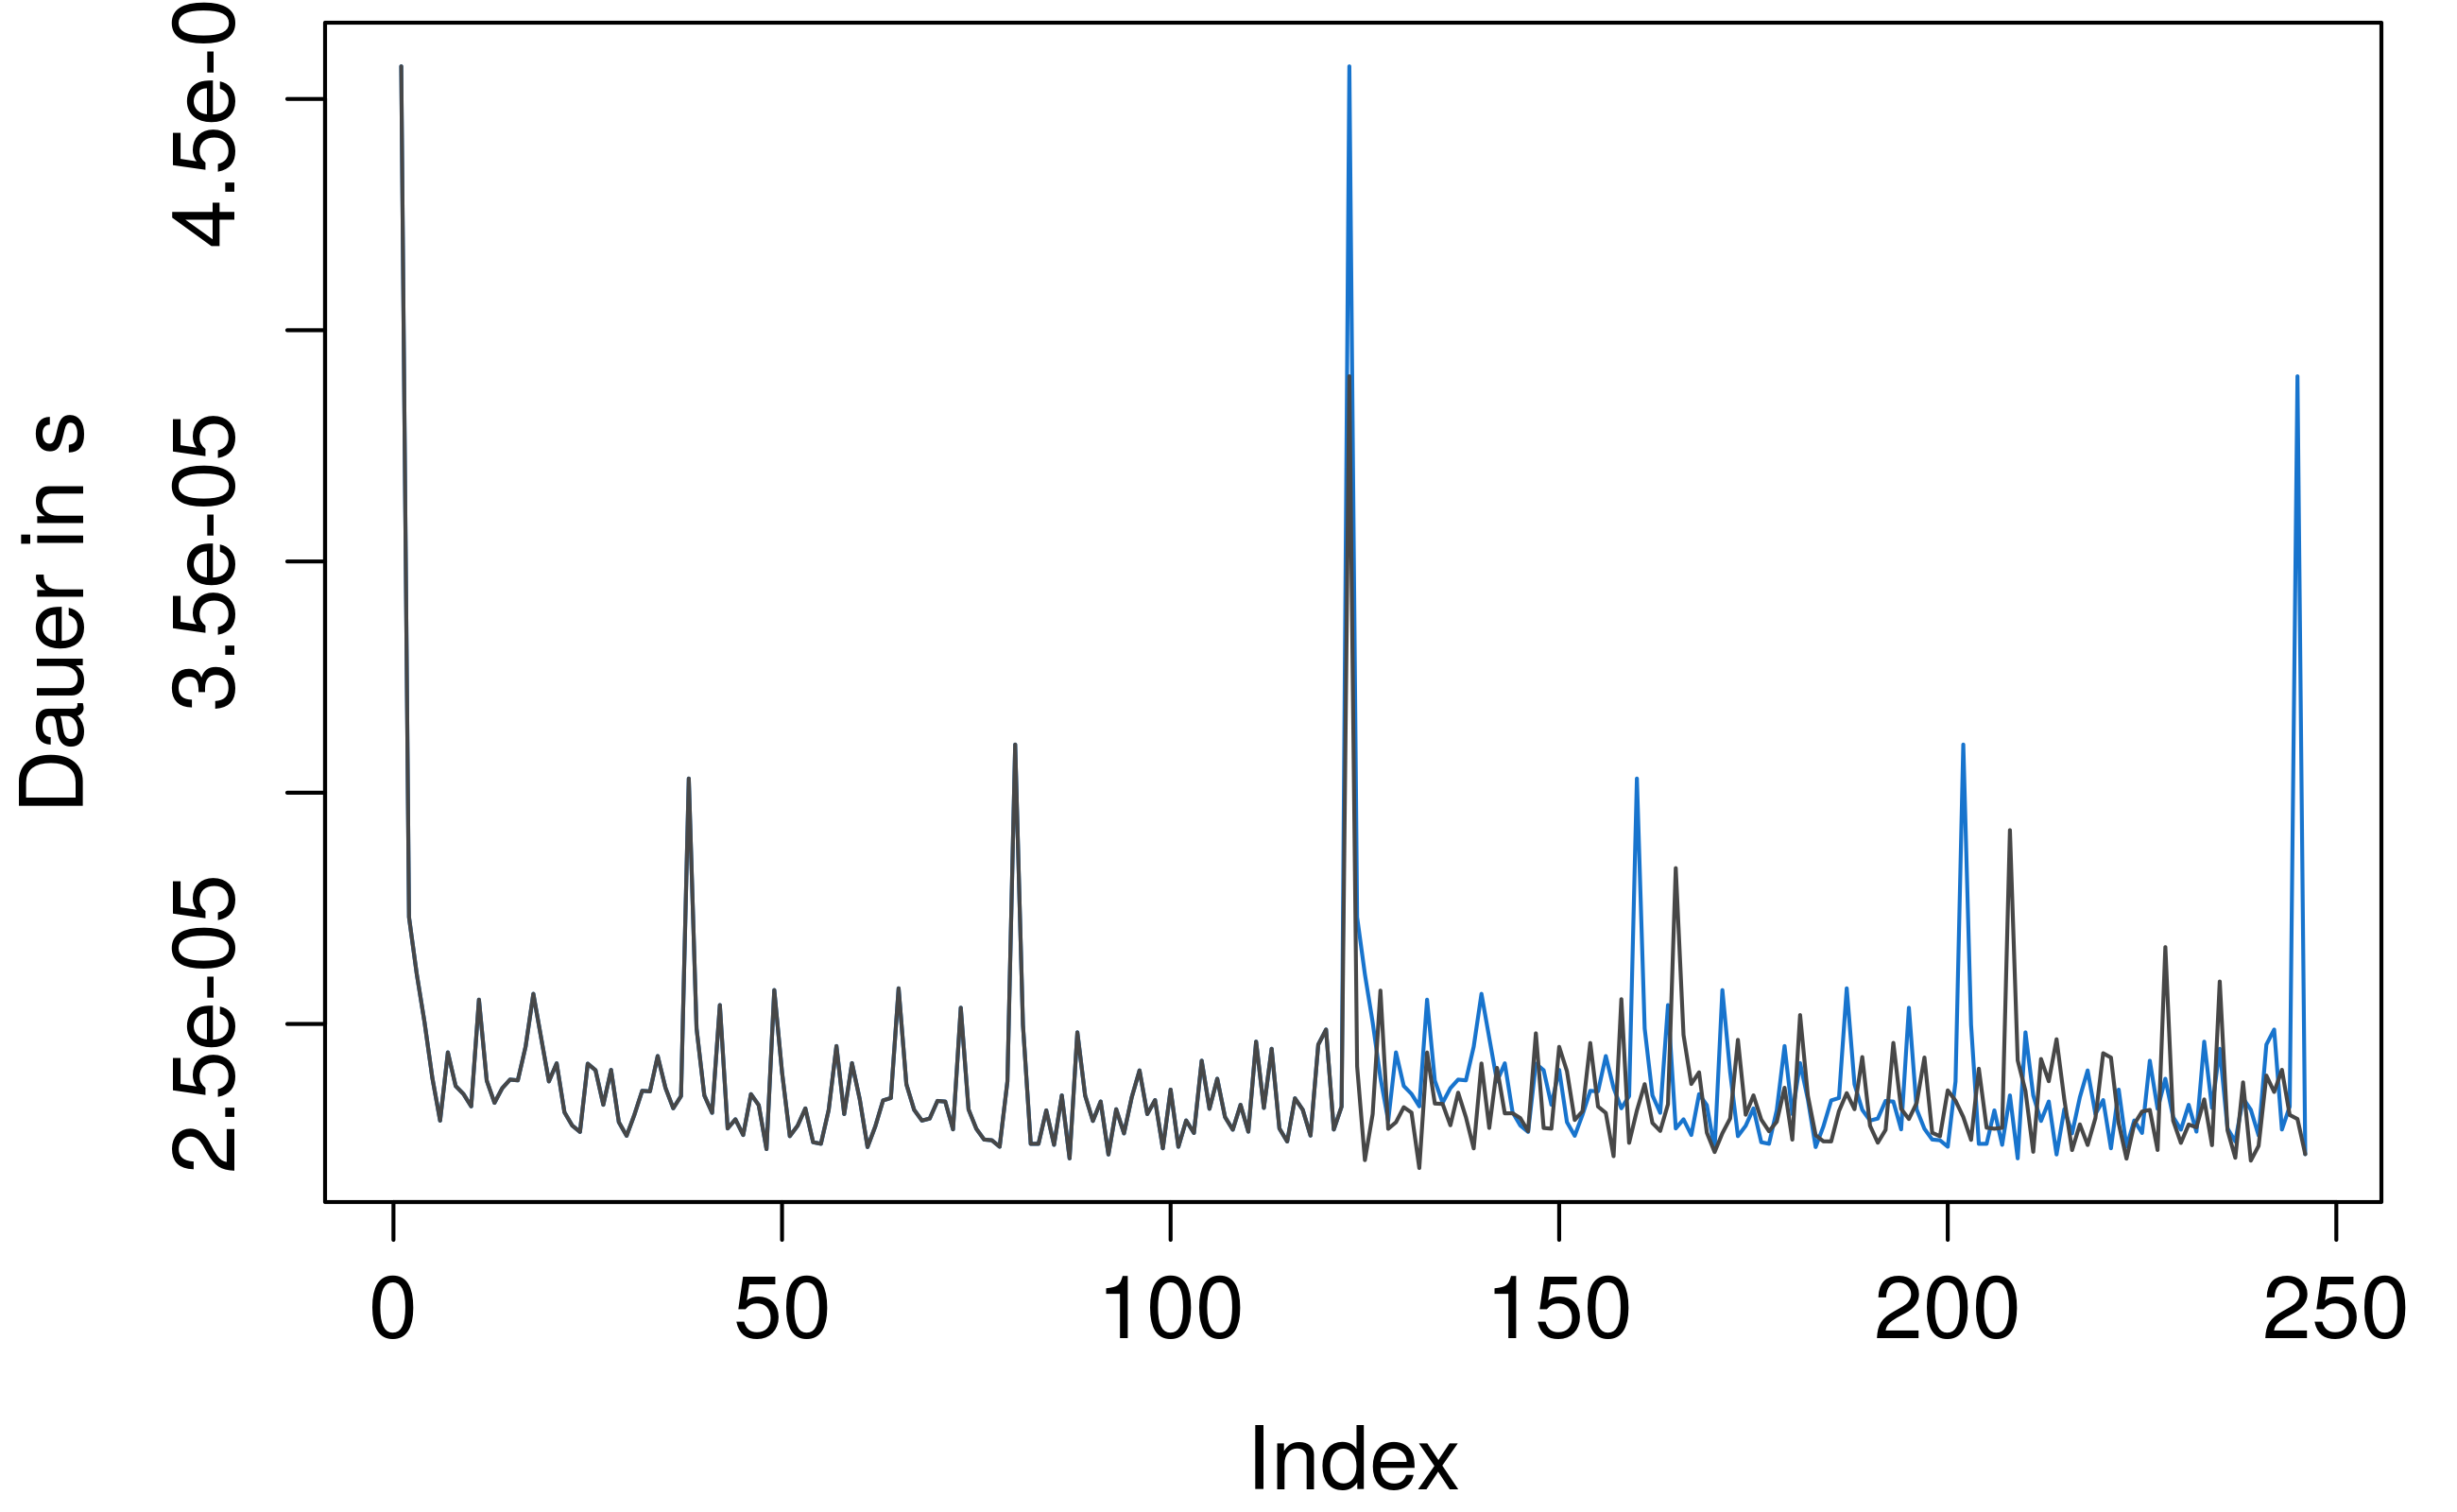
\includegraphics[width=0.6\textwidth]{Bilder/Plots/exploration/plot_periodicitywrite_seq.png}
		}	
		\caption{Ausnutzen des periodischen Verhaltens der Zugriffszeiten als erstes einfaches Modell}
		\label{fig:periodicity}
	\end{center}
\end{figure} 
\medskip

Eine weitere Detailbetrachtung mache ich willkürlich bei den Messungen 100001 bis 100250.
In diesem Fall scheint eine Periodizität in den Zugriffszeiten zu SEQ-R vorhanden zu sein. In Abbildung \ref{fig:periodicity100001} wurde eine Überlappung von Laufzeit und Vorhersage wie zuvor durchgeführt wird (diesmal werden die ersten 129 Messungen wiederholt). Man erkennt, dass dieses simple Modell die Ausreißer für diesen kleinen Ausschnitt tatsächlich exakt vorhersagen kann.\\
Im Allgemeinen kann dies jedoch offensichtlich nicht funktionieren.
Doch die Annahme einer gewissen Periodizität in der Leistung des E/A-Systems scheint gerechtfertigt zu sein.
Ein Modell, das versucht diese auszunutzen muss dabei eine komplexere Methode als schlichtes Übertragen vorheriger Leistungswerte ausnutzen, ansonsten kann es wohl nur in äußerst eingeschränktem Maße korrekte Leistung vorhersagen.

\begin{figure}
	\subfloat[Messungen 100001 bis 100250 in SEQ-R]{
		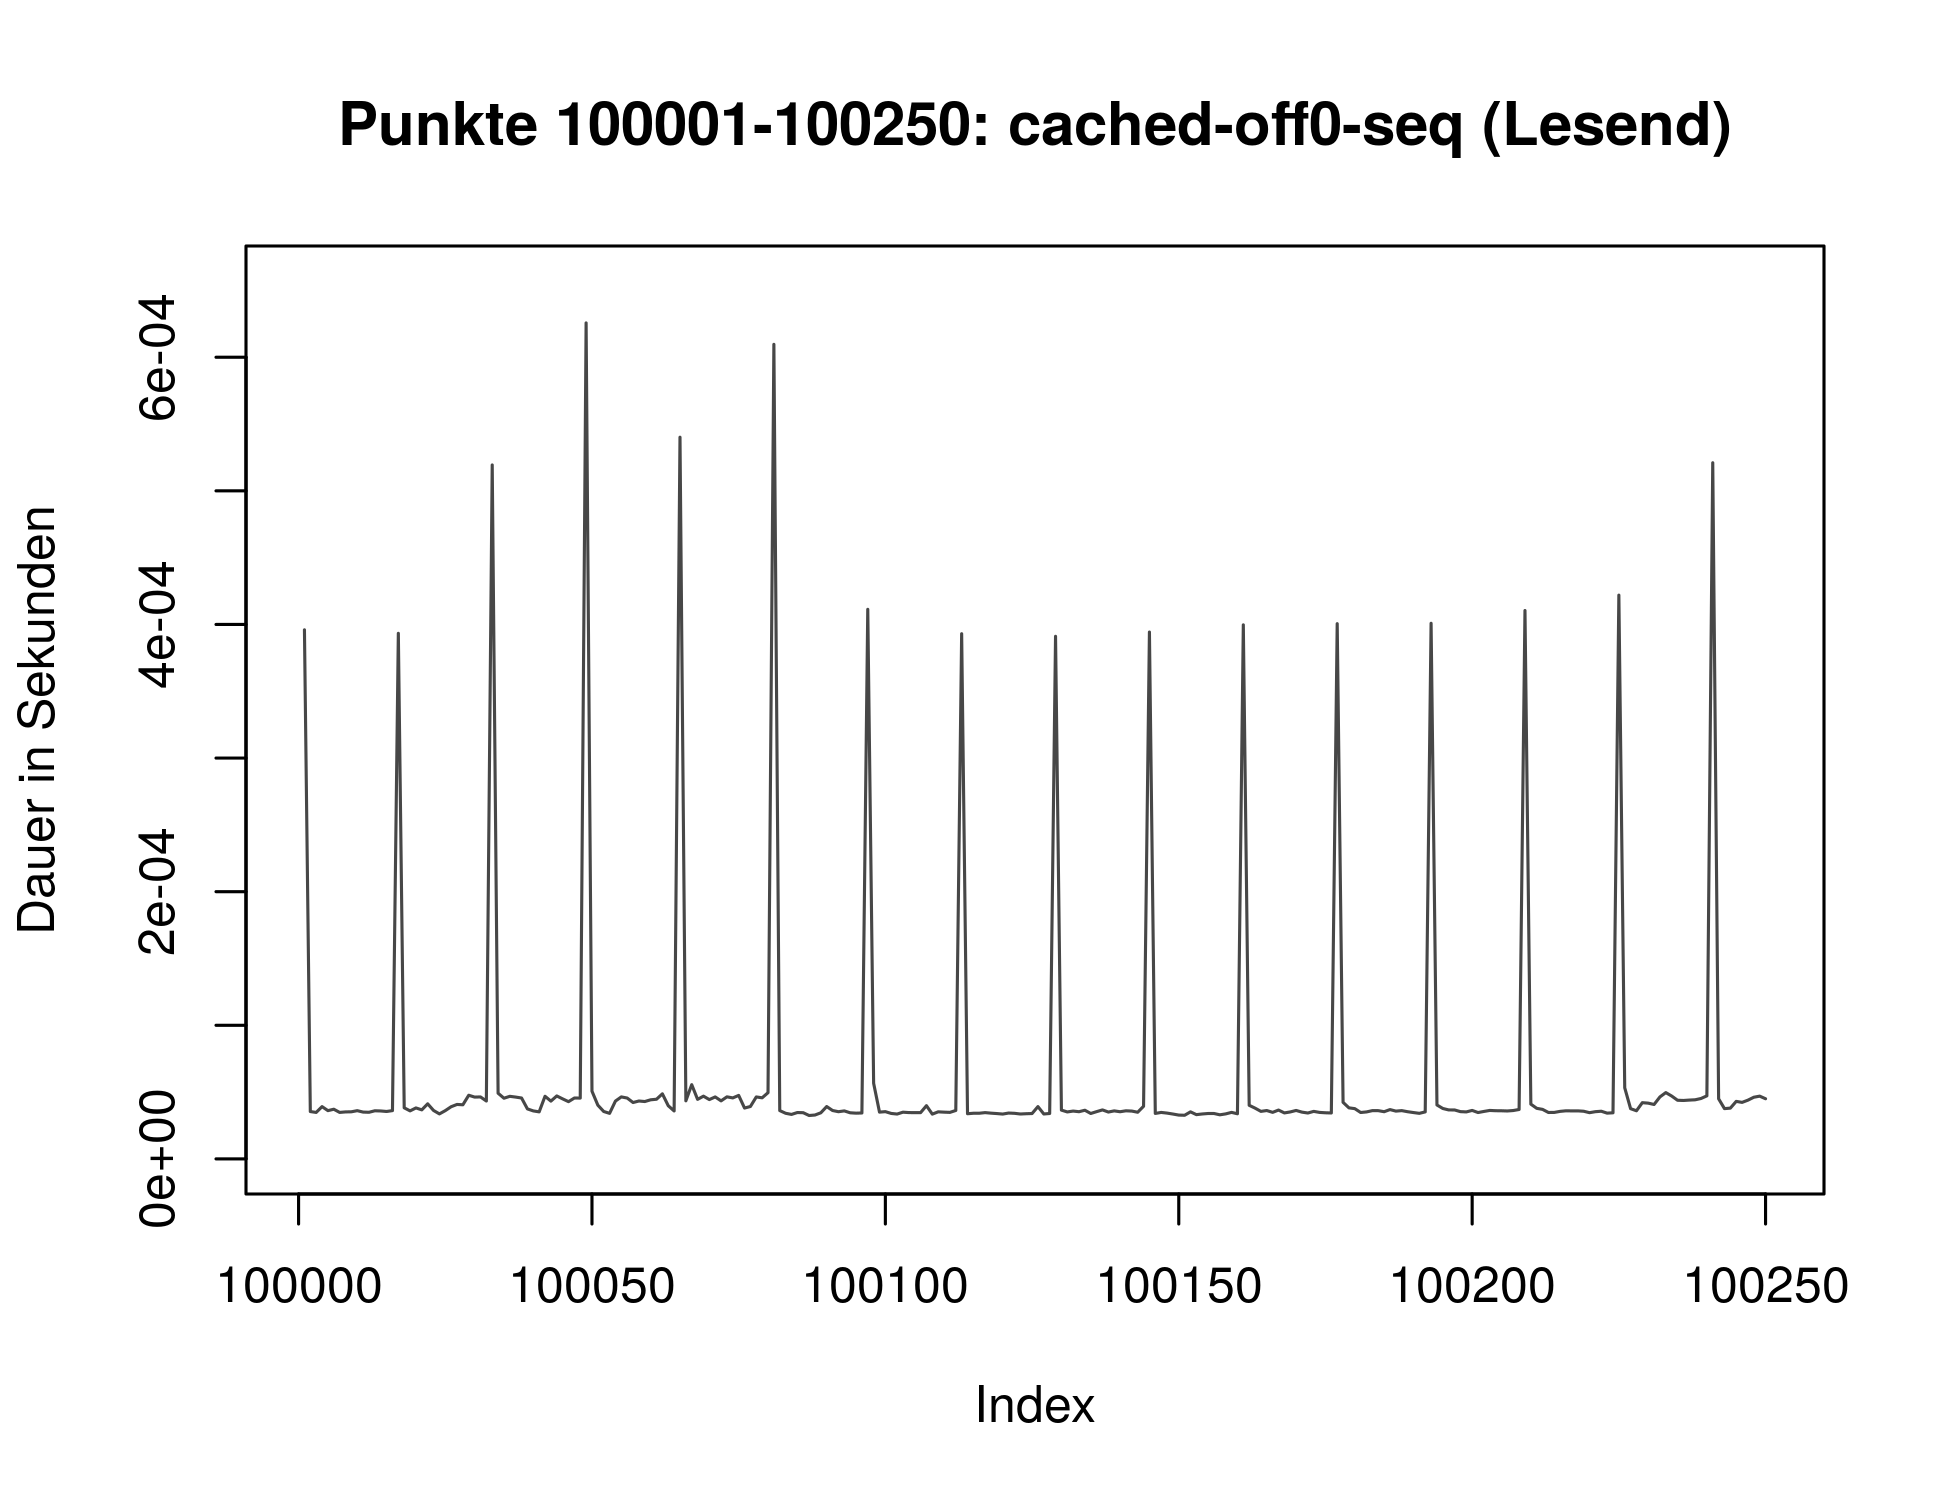
\includegraphics[width=.43\textwidth]{Bilder/Plots/exploration/plot_From100001to100250_read_seq.png}
	}
	\hfill
	\subfloat[Messungen 100001 bis 100250 in SEQ-W]{
		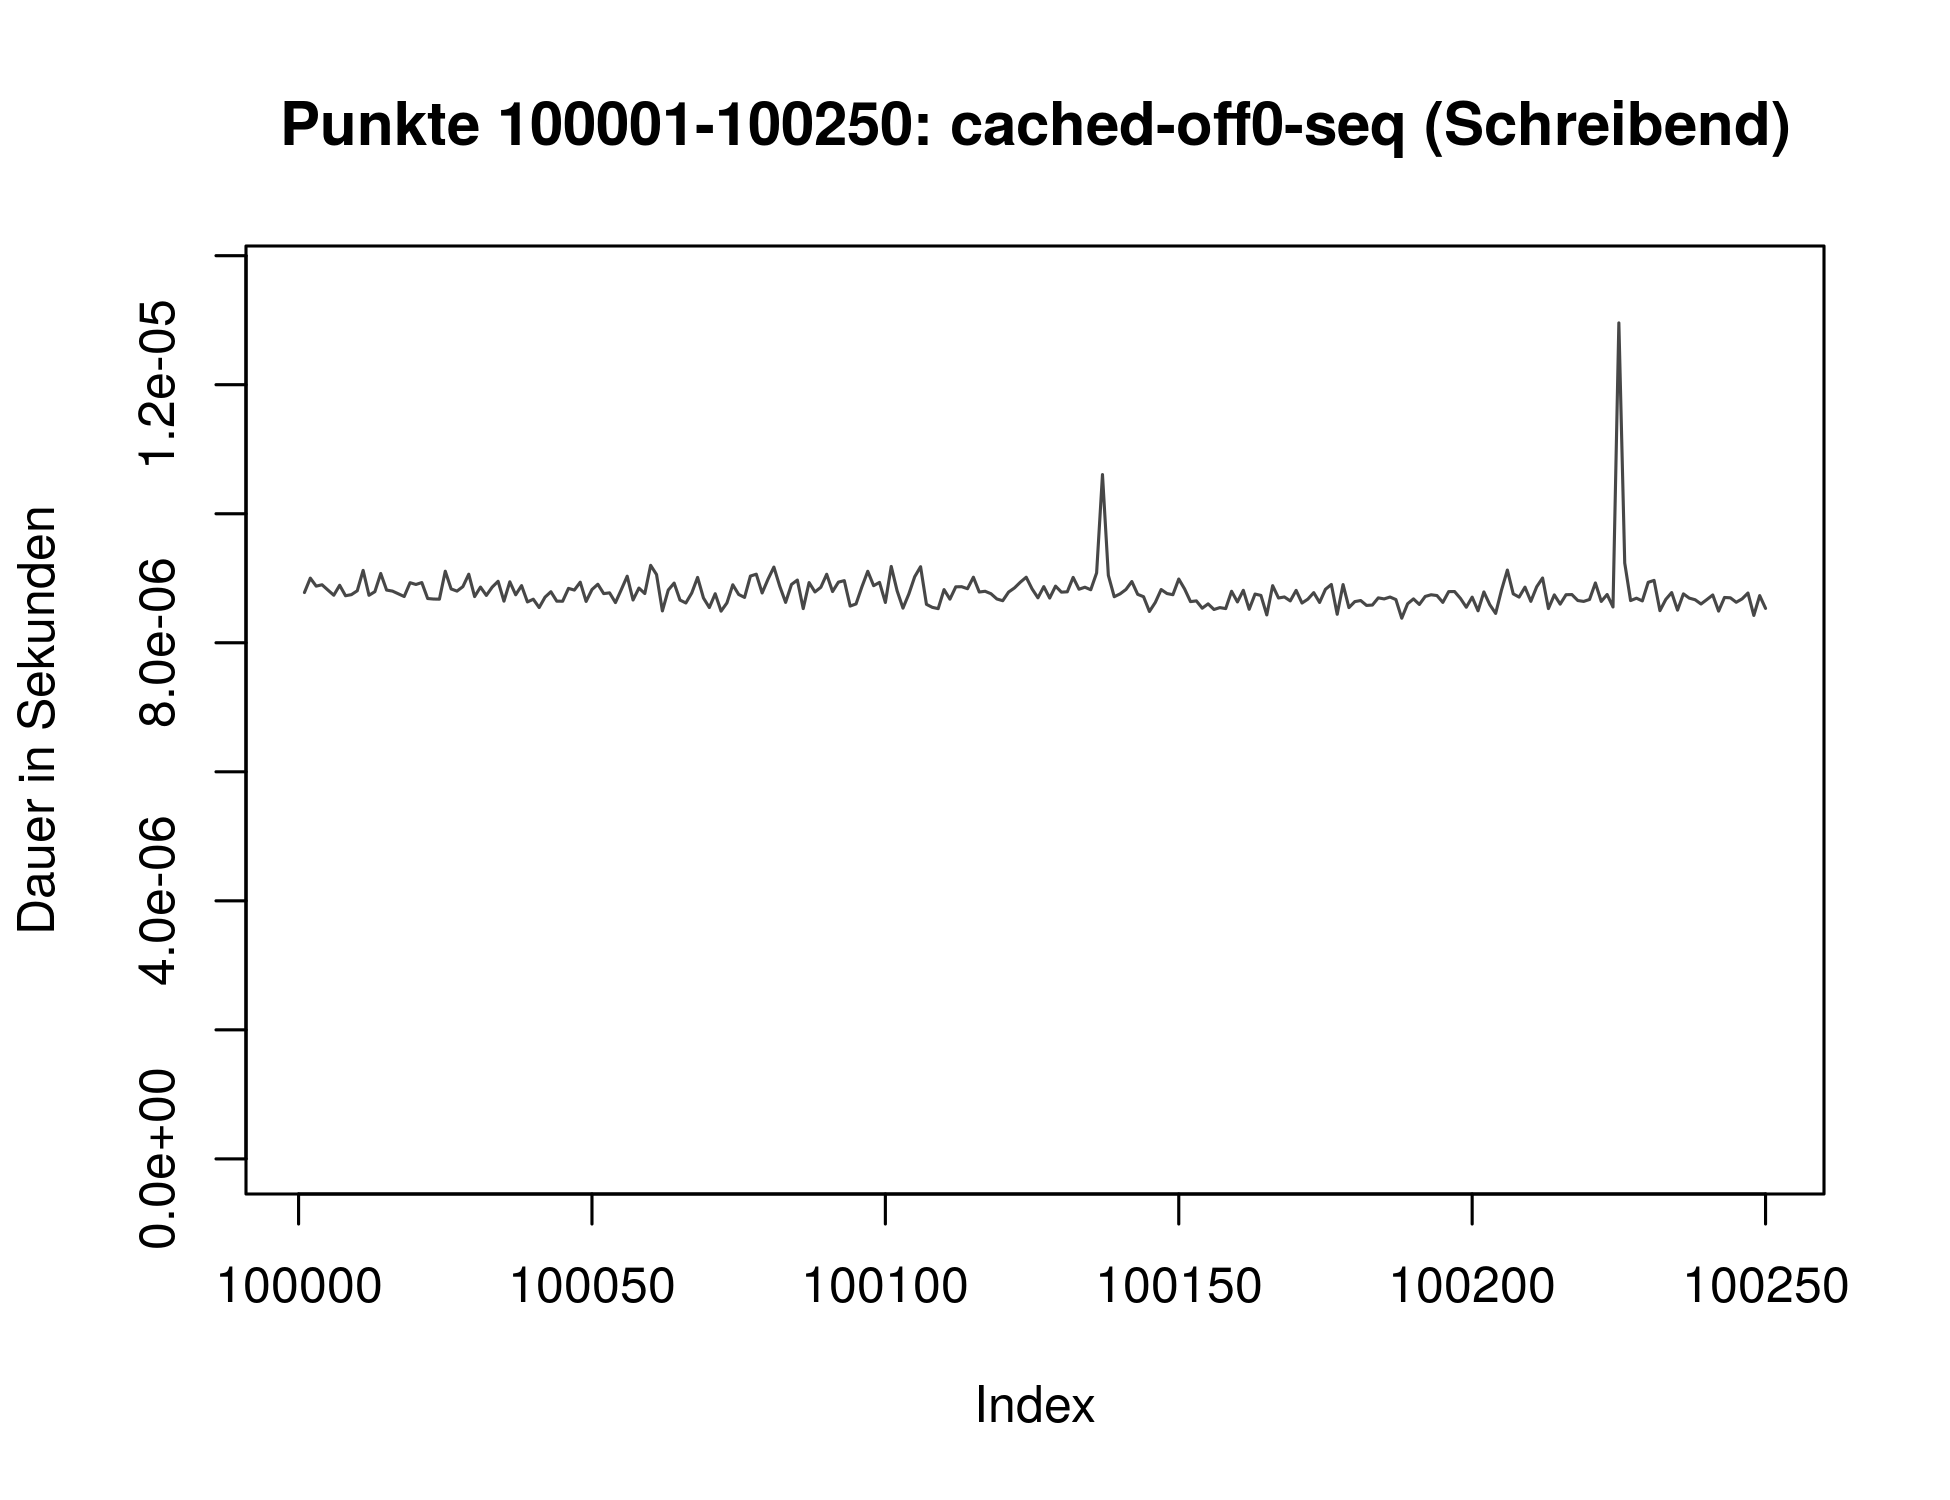
\includegraphics[width=.43\textwidth]{Bilder/Plots/exploration/plot_From100001to100250_write_seq.png}
	}\\
	\subfloat[Messungen 100001 bis 100250 in RND-R]{
		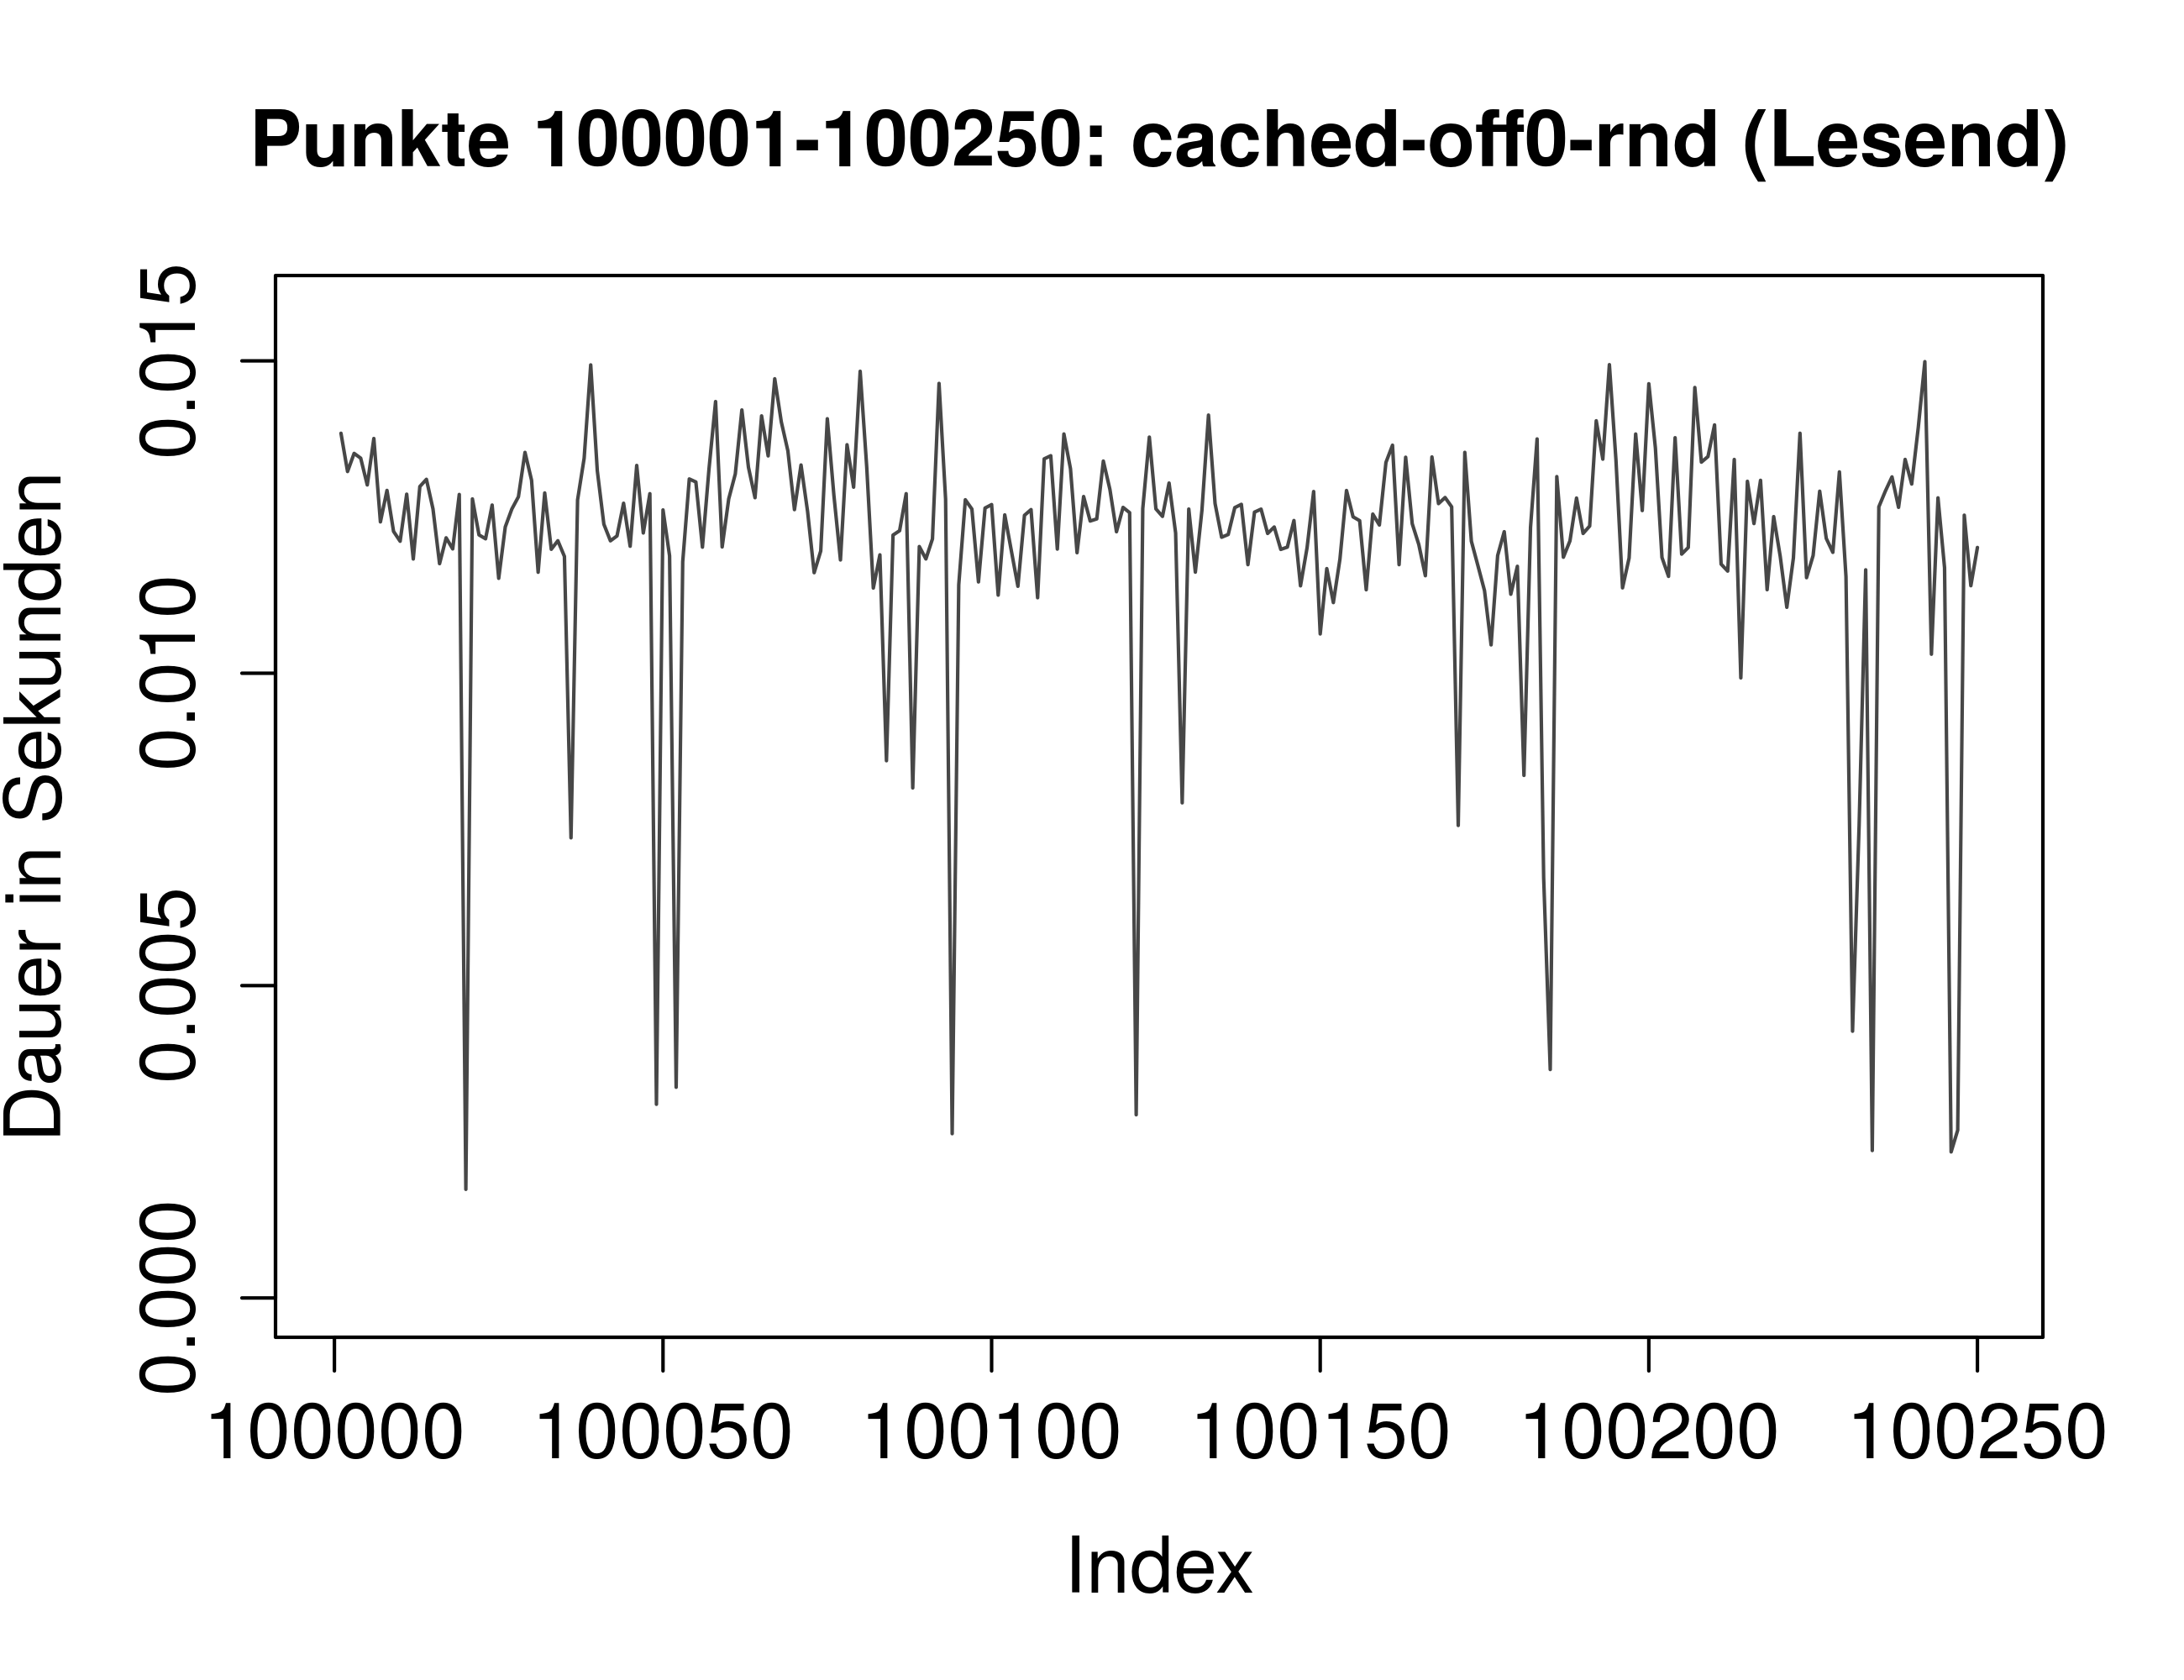
\includegraphics[width=.43\textwidth]{Bilder/Plots/exploration/plot_From100001to100250_read_rnd.png}
	}
	\hfill
	\subfloat[Messungen 100001 bis 100250 in RND-W]{
		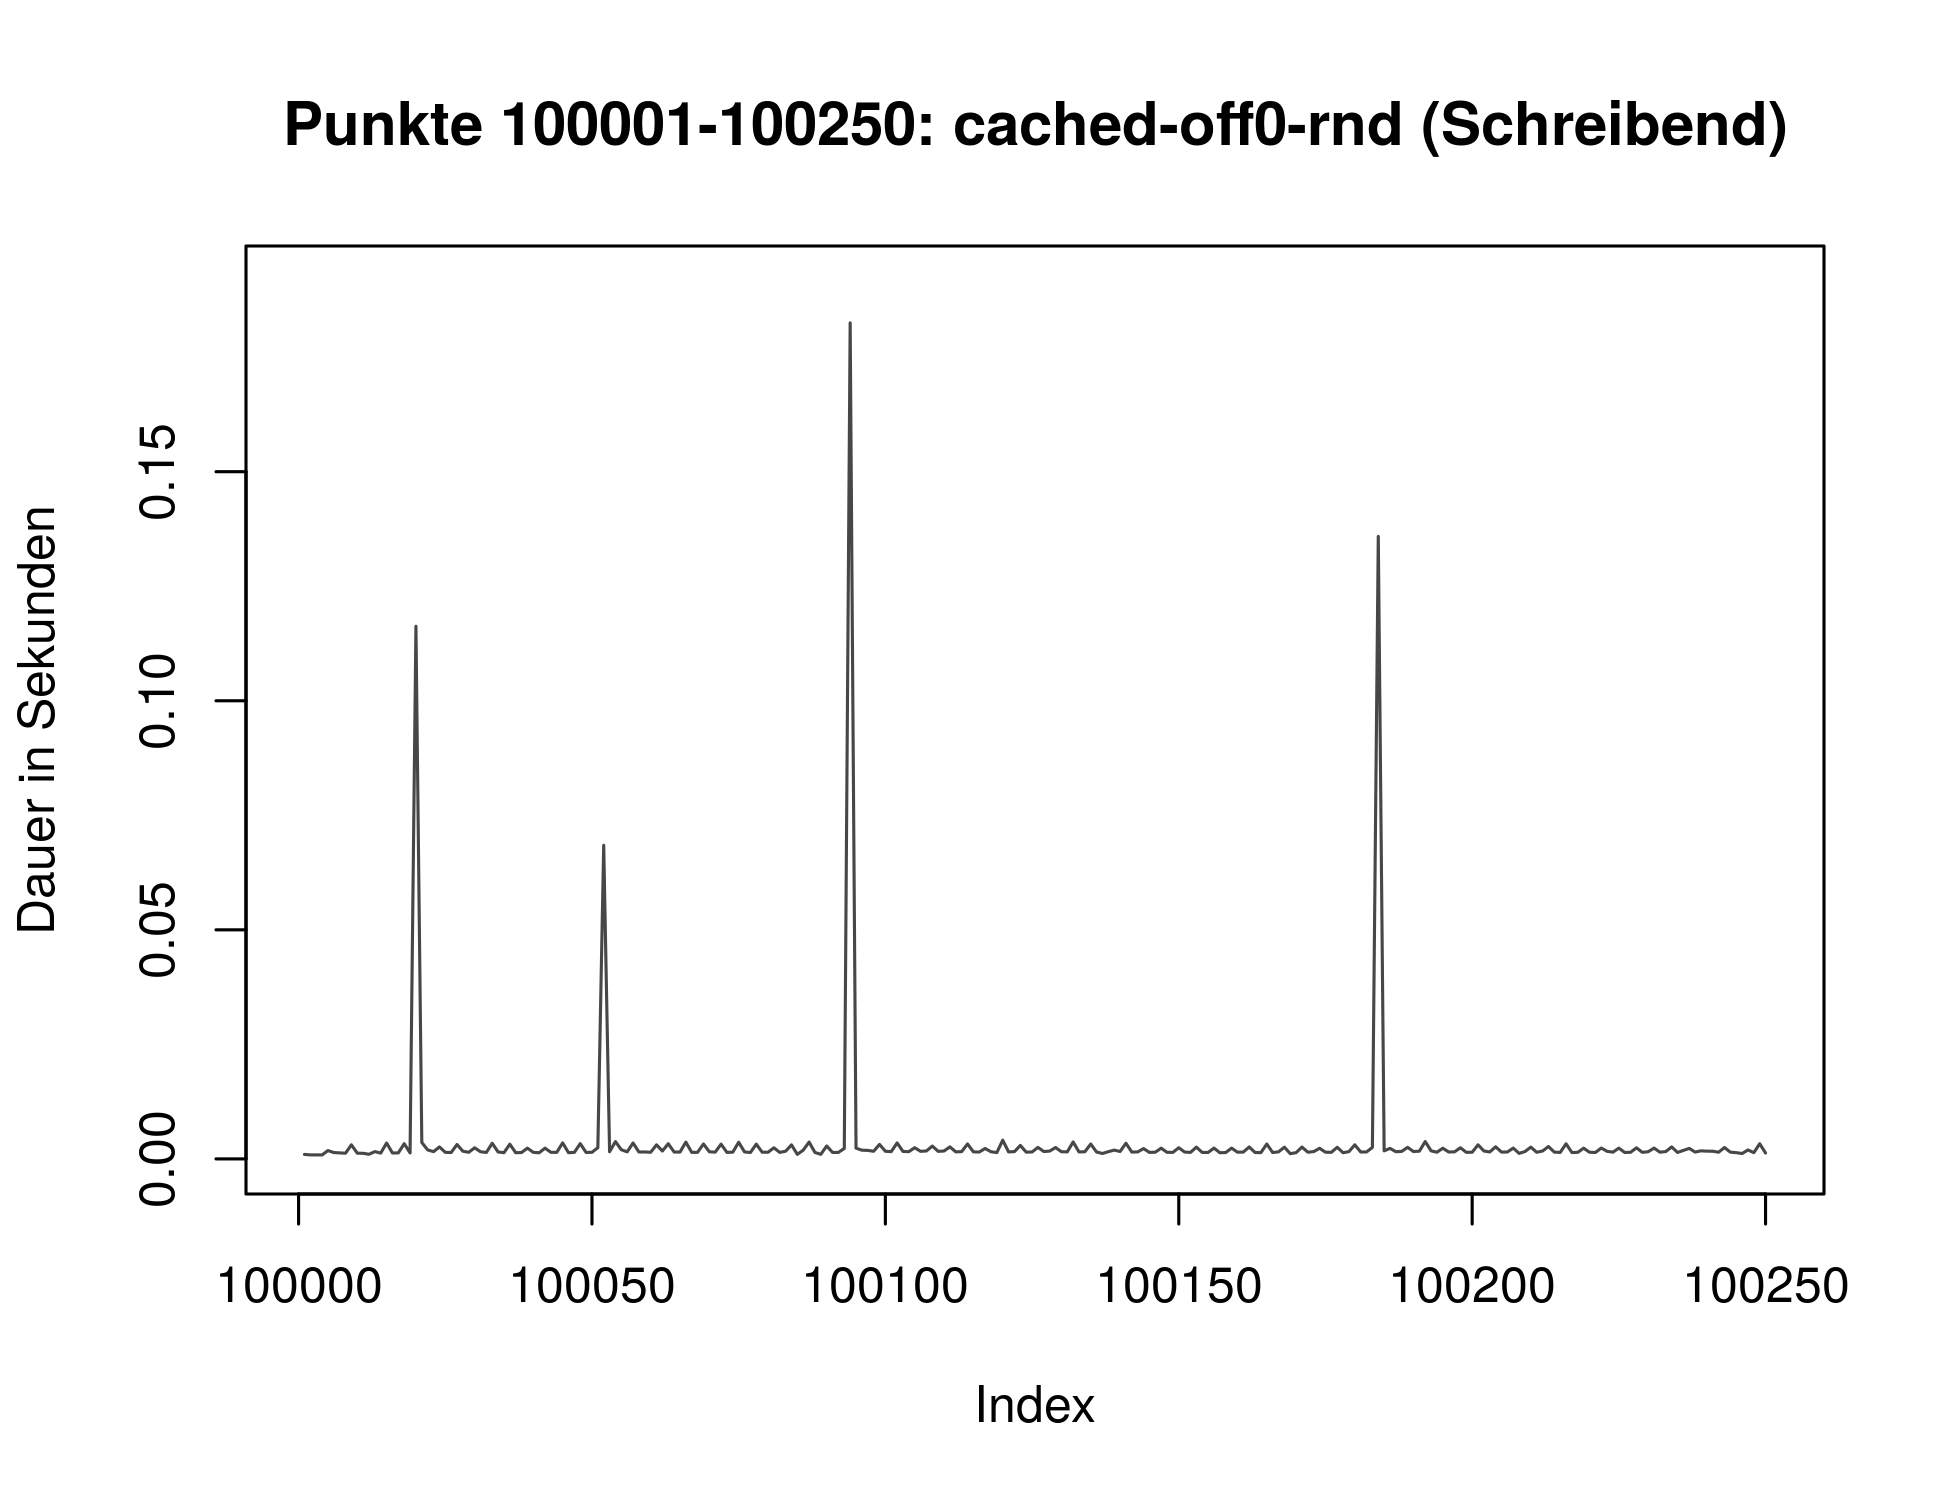
\includegraphics[width=.43\textwidth]{Bilder/Plots/exploration/plot_From100001to100250_write_rnd.png}
	}		
	\caption{Detailbetrachtung der Messungen 100001 bis 100250}
	\label{fig:from100001}
\end{figure} 

\begin{figure}
	\begin{center}
		\subfloat{
			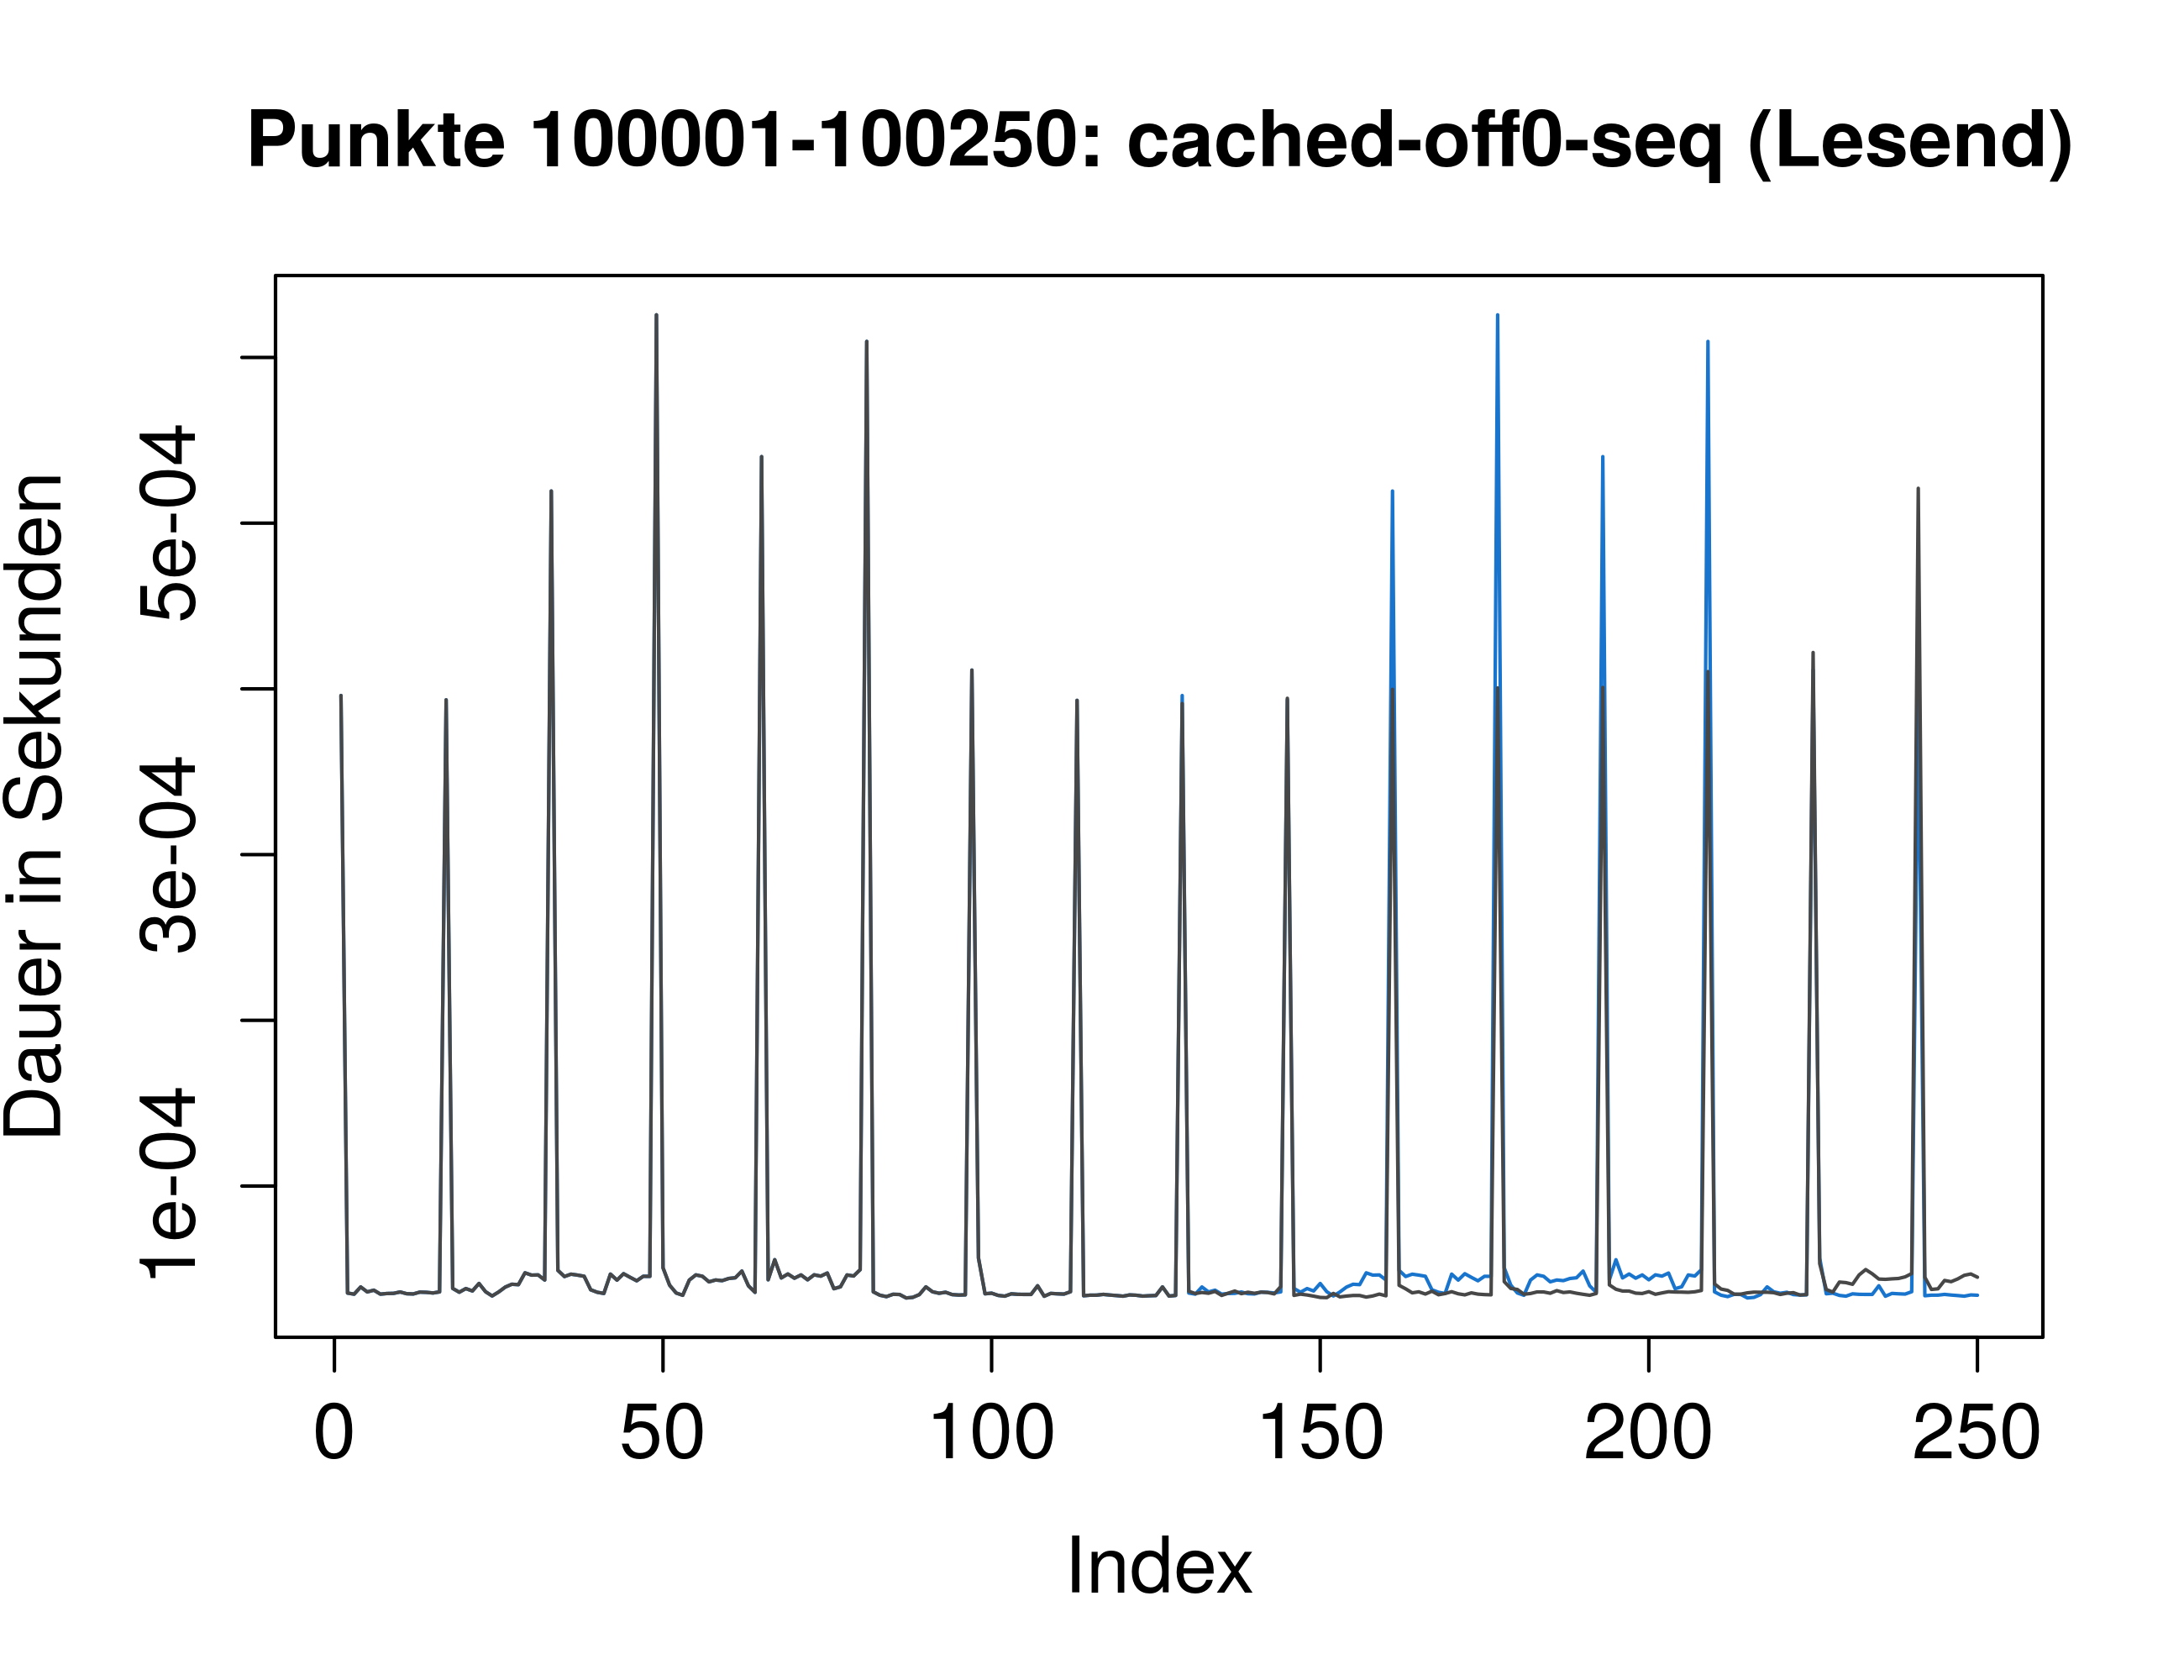
\includegraphics[width=.6\textwidth]{Bilder/Plots/exploration/plot_periodicity100001read_seq.png}
		}	
		\caption{Ausnutzen des periodischen Verhaltens der Zugriffszeiten als erstes einfaches Modell}
		\label{fig:periodicity100001}
	\end{center}
\end{figure} 
\clearpage

\section{Analyse der Fehlerklassen}
\label{eval:fk_analyse}
Alle Modelle werden auf den zusammengeführten Datensätzen aus lesenden und schreibenden Zugriffen angewendet. Daher gibt es im Folgenden nur noch jeweils eine Abbildung zu den sequentiellen und eine zu den Messungen mit zufälligem Dateizugriff.
Zunächst werden zu einer Zugriffsgröße alle Messreihen mit lesenden Aufrufen gezeichnet, danach kommen die schreibenden Zugriffe. 
Die in \ref{fk-modelle} eingeführten Fehlerklassen untersuche ich anhand der Ergebnisse, die aus der Clusteranalyse der Residuen von \textit{LinReg G} entstanden sind.\medskip

In \ref{fig:error_class_clustering_seq}a, sowie \ref{fig:error_class_clustering_rnd}a sind in Zeitreihe die Residuen aufgezeichnet, die \textit{LinReg G} auf den sequentiell, respektive randomisiert ausgeführten Messungen, mit seinen Vorhersagen gegenüber den tatsächlichen Laufzeiten erreicht hat.
Das Modell \textit{LinReg G} kann nicht zwischen den Operationsarten unterscheiden, auf SEQ führt dies zu etwa gleichen Modellabweichungen für lesende und schreibende Zugriffe, auf RND werden die weit verstreuten Laufzeiten zu lesenden Zugriffen schlechter approximiert.
Die absolute Abweichung wächst bei sequentiellen Zugriff mit der Größe der E/A-Aufrufe, für die zufälligen Zugriffe gilt dies nur bedingt. Auf den kleinsten Zugriffsgrößen werden kleine Fehler gemacht, danach bleibt der Betrag in etwa auf einem Niveau.
Ein Grund für höhere Abweichungen bei Messungen mit längeren Zugriffszeiten ist, dass ein bestimmter relativer Fehler zu entsprechend höheren absoluten Fehlern führt.
Für den plötzlichen und sehr starken Anstieg der Residuen auf höheren Zugriffsgrößen kann dies aber vermutlich nicht die einzige Erklärung sein.

\begin{figure}
	\centering
	\subfloat[Residuen von \textit{LinReg G} auf SEQ]{
		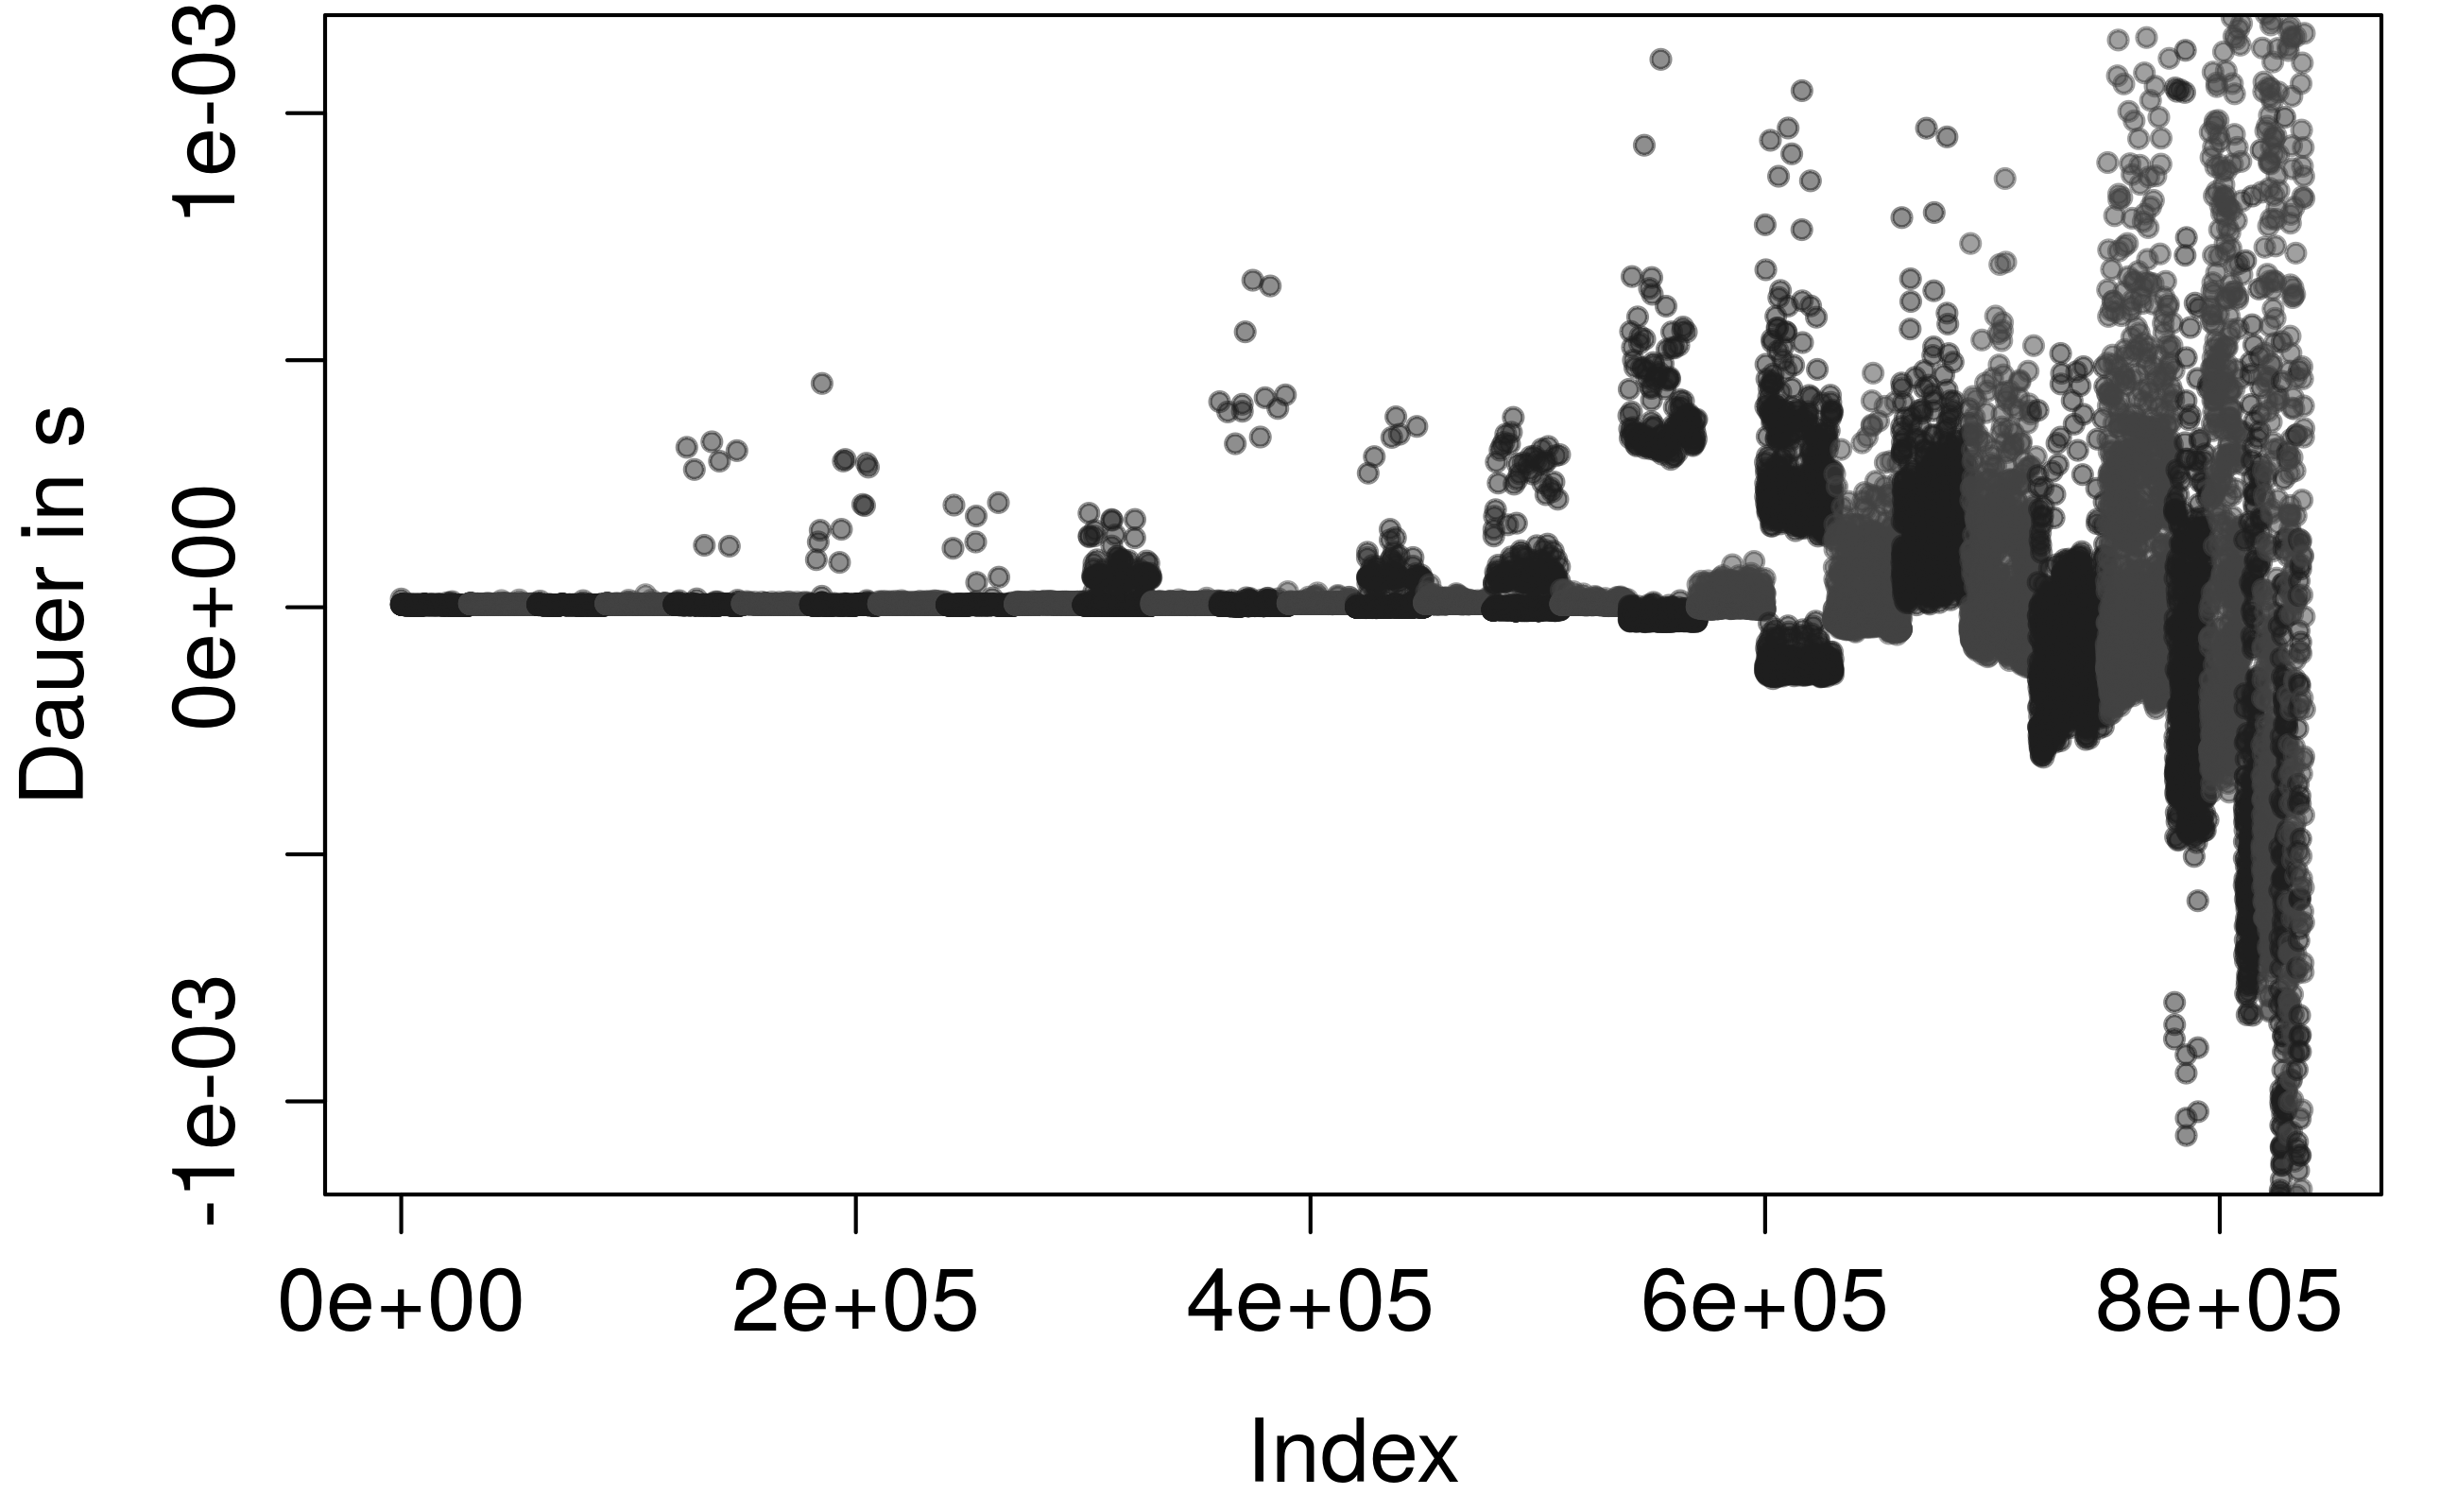
\includegraphics[width=.40\textwidth]{Bilder/Plots/error_class/exploration/linreg_error_seq_all.png}
	}\hfill
	\subfloat[Farblich markierte Fehlerklassen]{
		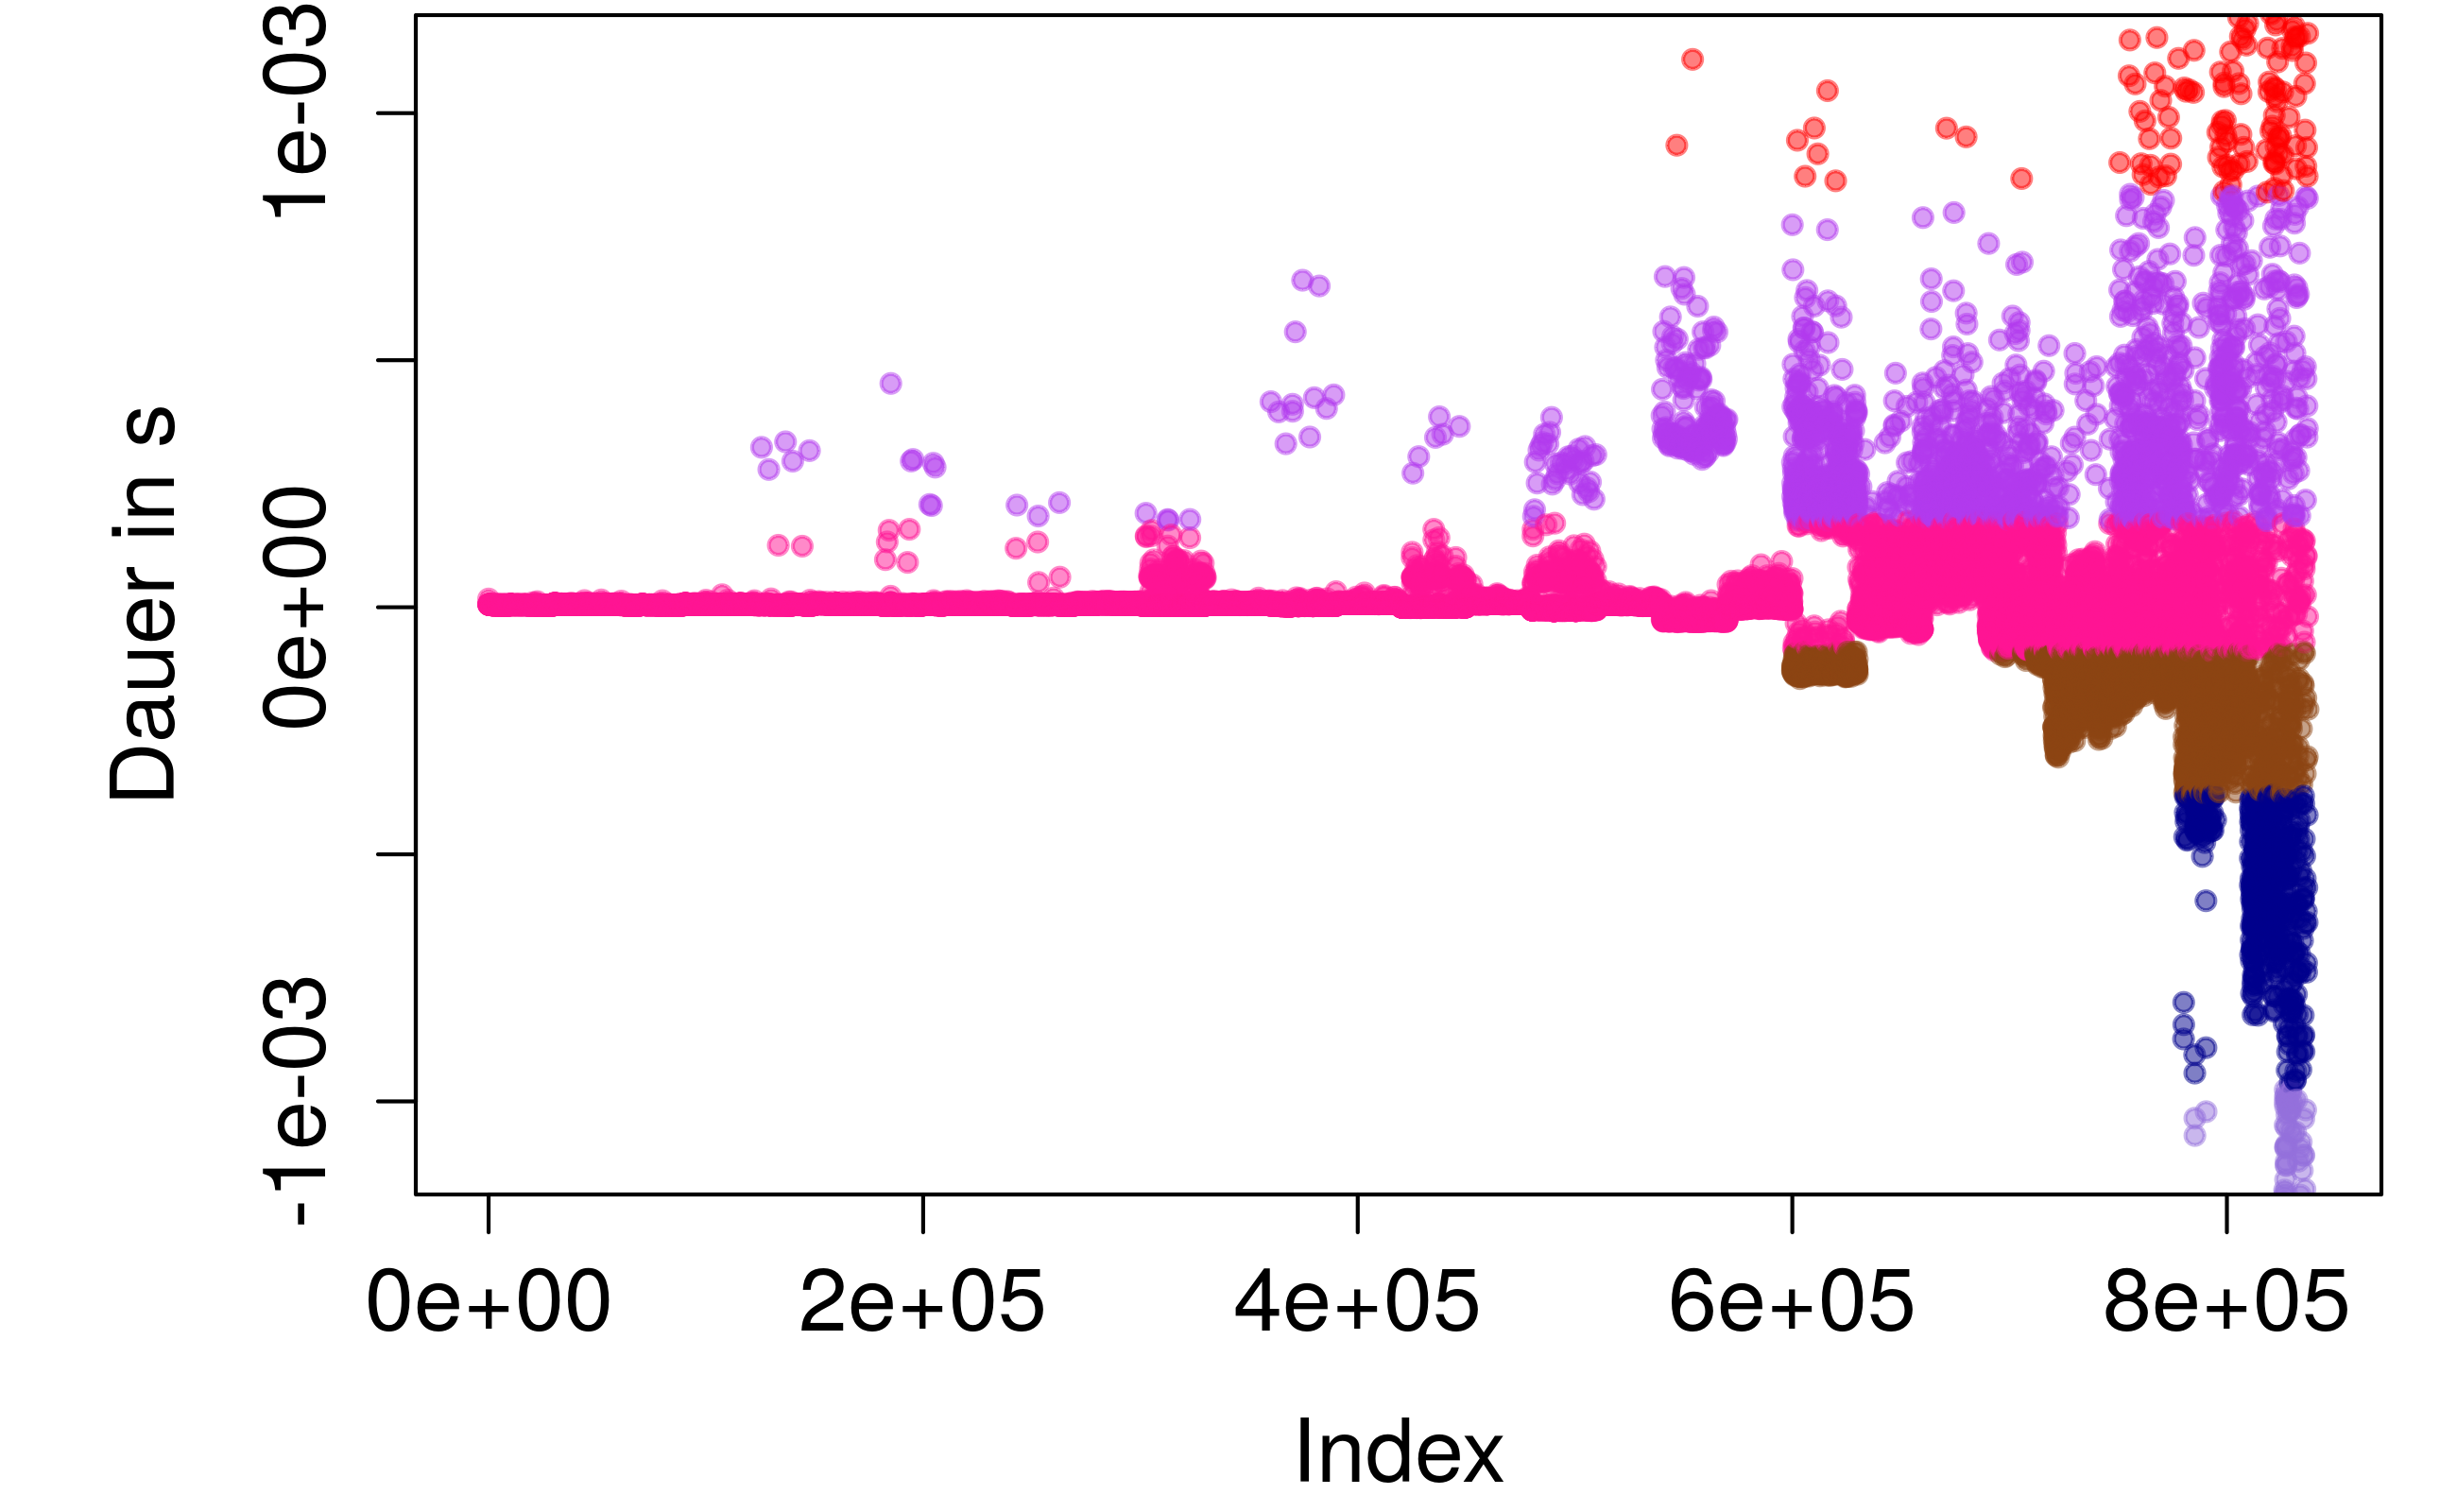
\includegraphics[width=.40\textwidth]{Bilder/Plots/error_class/exploration/linreg_error_clustering_seq_all.png}
	}\\
	\subfloat[Residuen sortiert nach Modellabweichung]{
		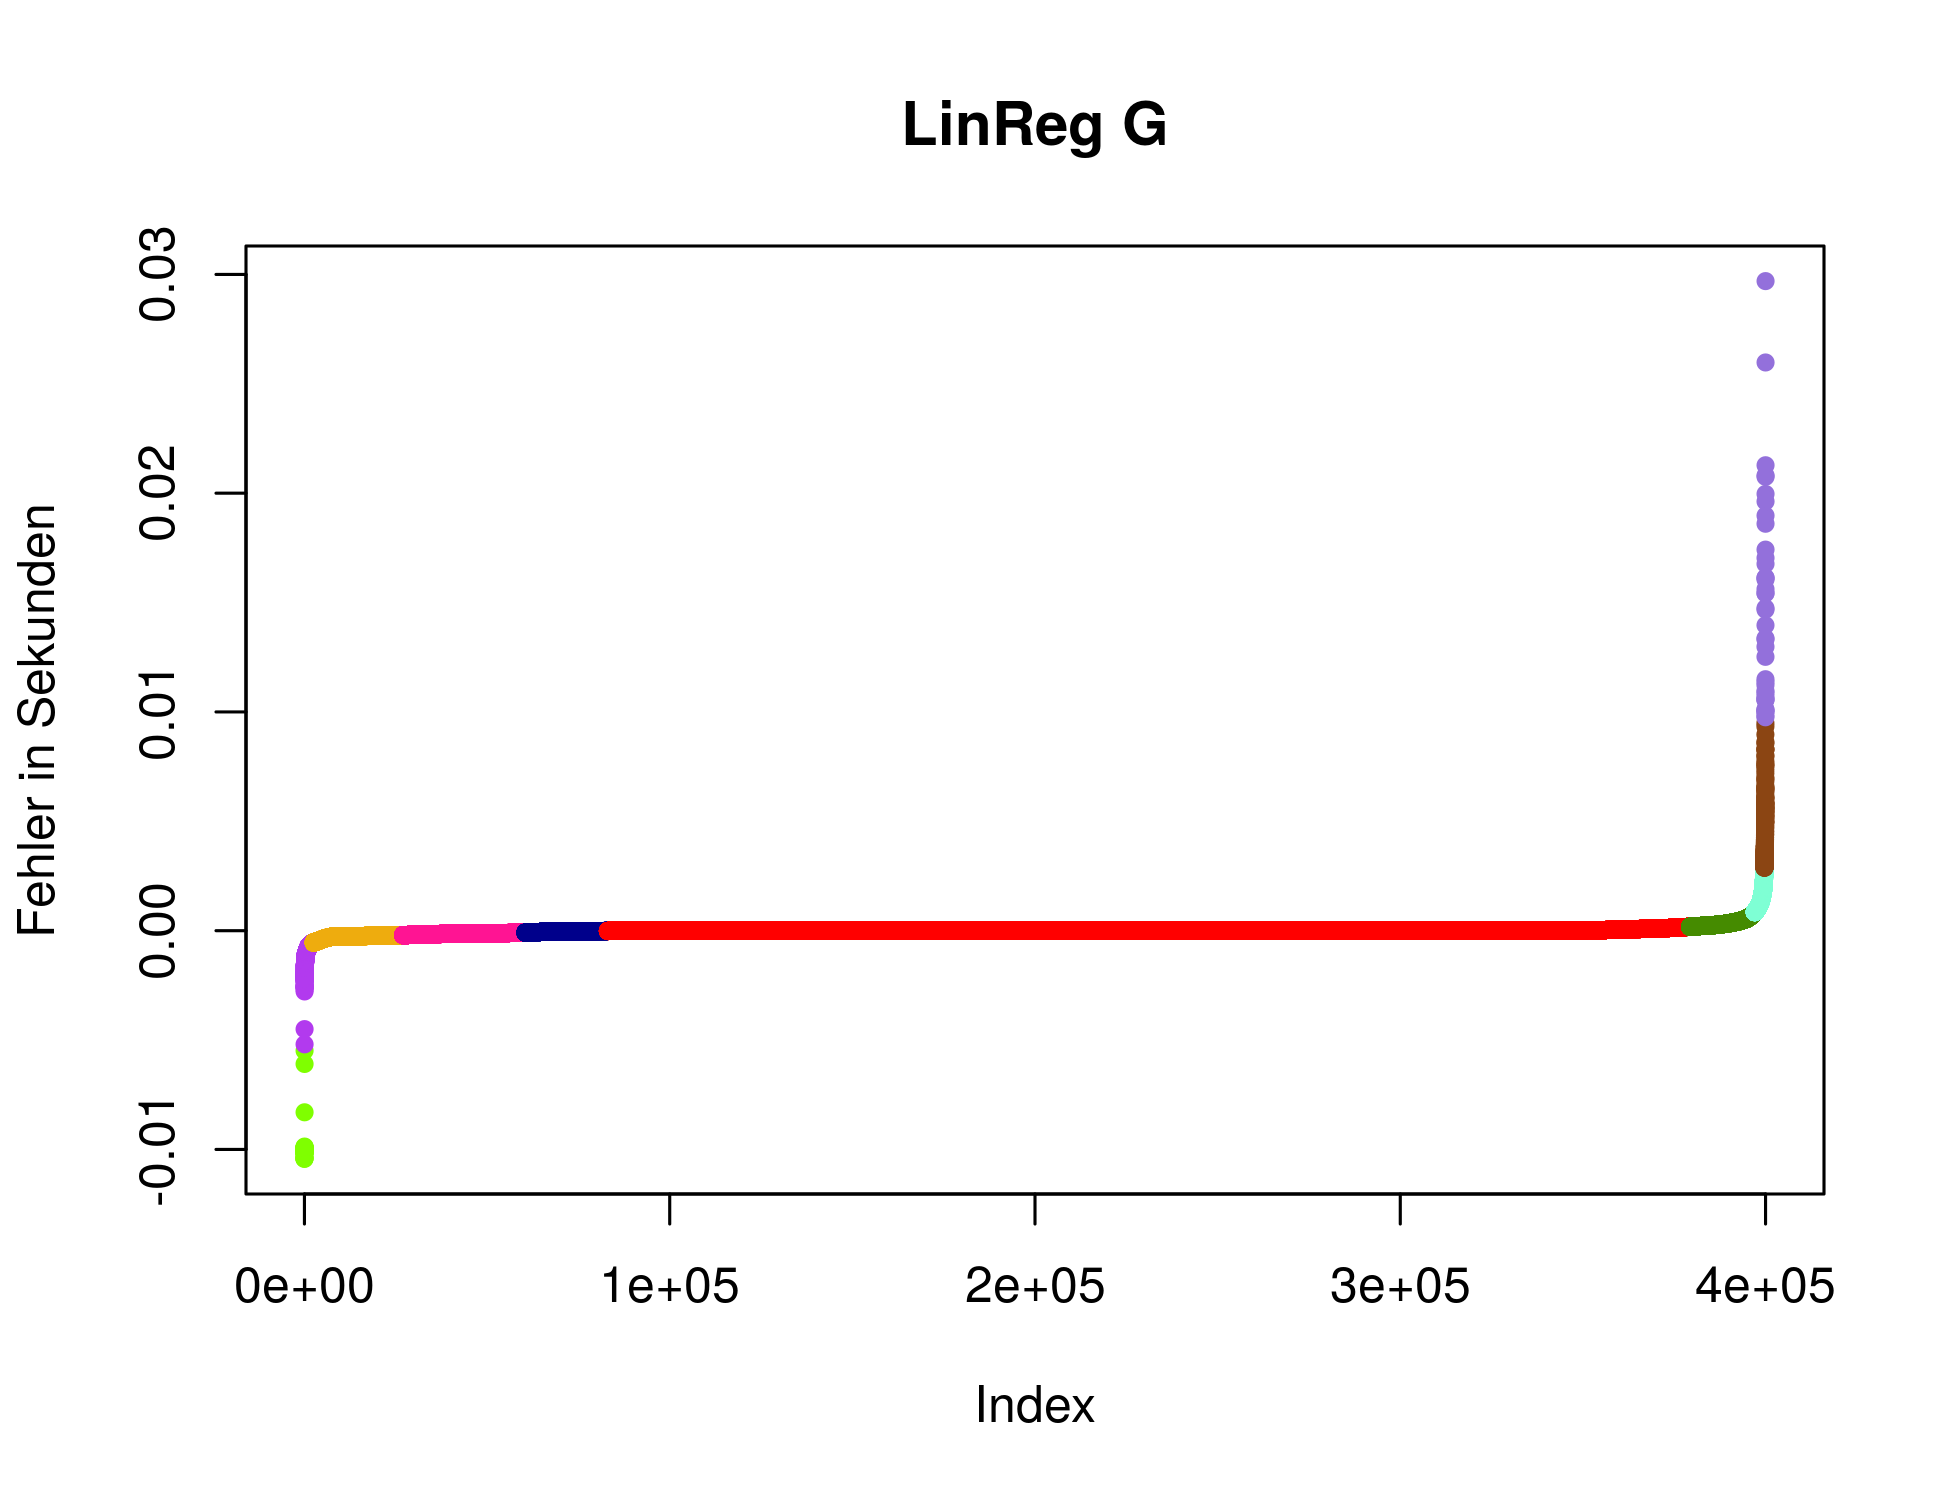
\includegraphics[width=.40\textwidth]{Bilder/Plots/error_class/exploration/linreg_error_sorted_clustering_seq.png}
	}\hfill
	\subfloat[Dichte der drei Klassen um den Nullpunkt]{
		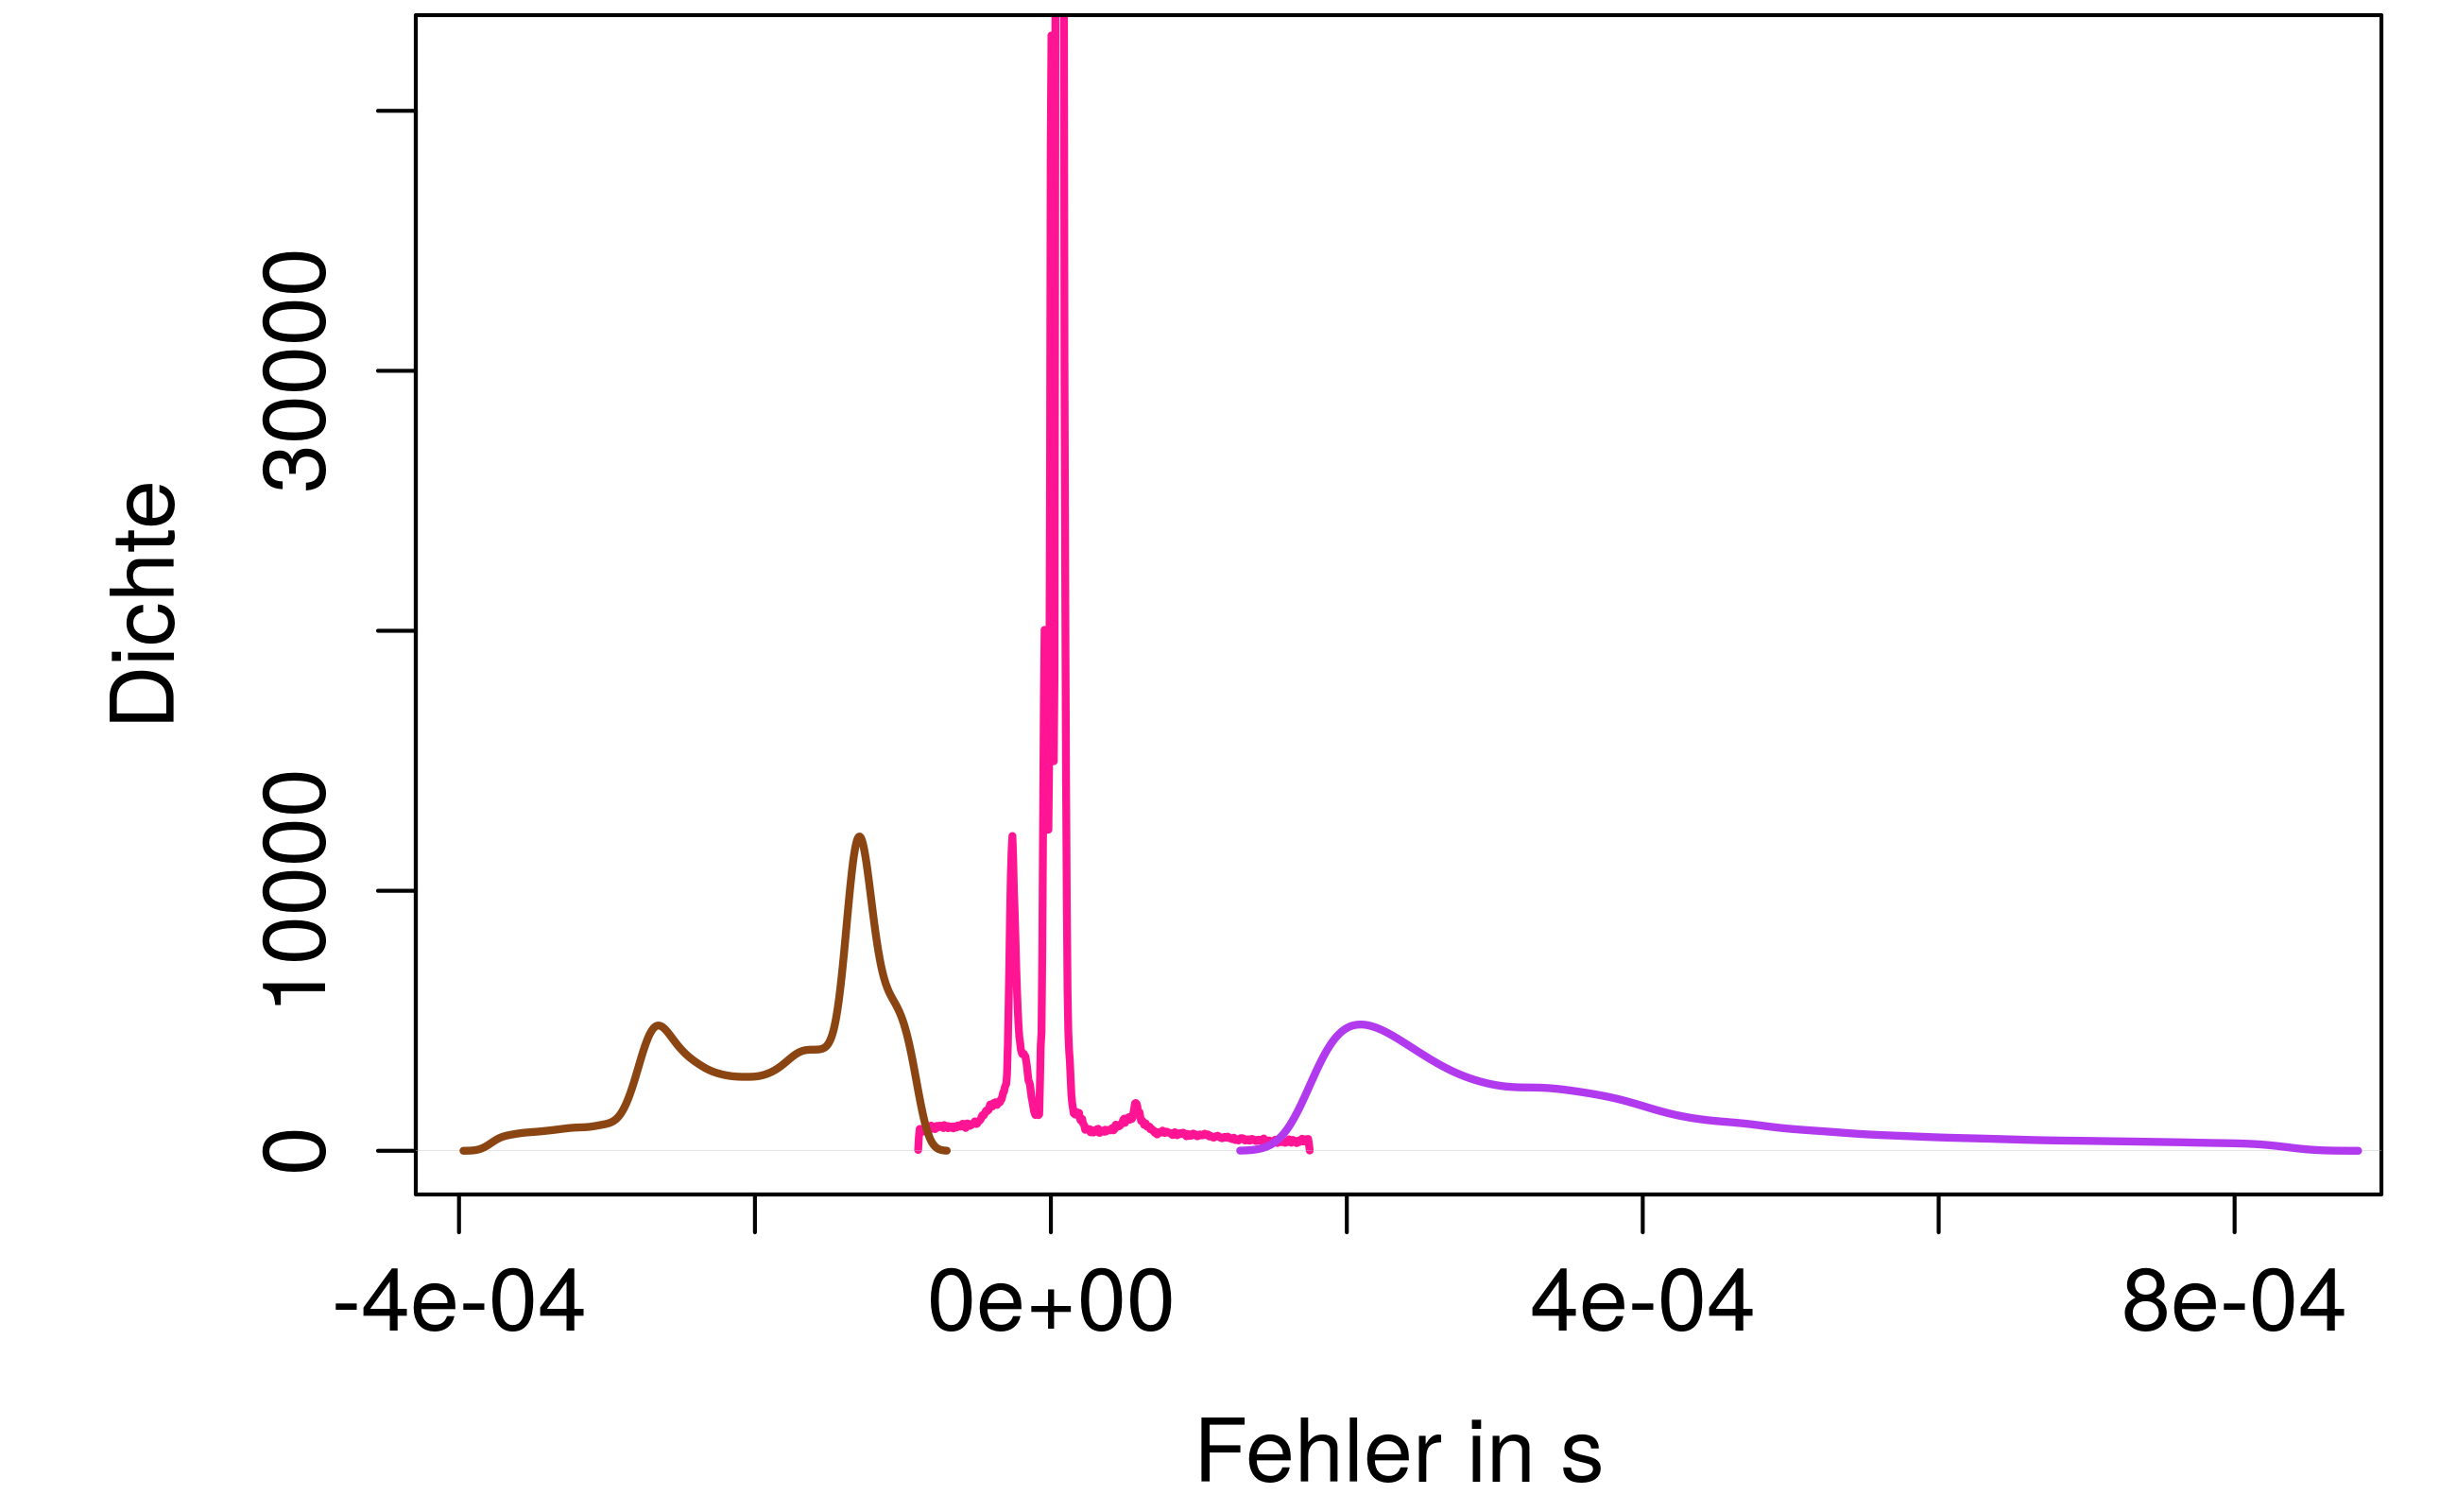
\includegraphics[width=.40\textwidth]{Bilder/Plots/error_class/exploration/density_of_fk_seq.png}
	}
	\vspace*{-0.3cm}
	\caption{Fehlerklassen, die aus den Residuen von \textit{LinReg G} auf SEQ durch Clustering erstellt wurden}
	\label{fig:error_class_clustering_seq}
\end{figure} 
\begin{figure}
	\centering
	\subfloat[Residuen von \textit{LinReg G} auf RND]{
		\includegraphics[width=.40\textwidth]{Bilder/Plots/error_class/exploration/linreg_error_rnd_all.png}
	}\hfill
	\subfloat[Farblich markierte Fehlerklassen]{
		\includegraphics[width=.40\textwidth]{Bilder/Plots/error_class/exploration/linreg_error_clustering_rnd_all.png}
	}\\
	\subfloat[Residuen sortiert nach Modellabweichung]{
		\includegraphics[width=.40\textwidth]{Bilder/Plots/error_class/exploration/linreg_error_sorted_clustering_rnd.png}
	}\hfill
	\subfloat[Dichte der drei Klassen um den Nullpunkt]{
		\includegraphics[width=.40\textwidth]{Bilder/Plots/error_class/exploration/density_of_fk_rnd.png}
	}
	\vspace*{-0.3cm}
	\caption{Fehlerklassen, die aus den Residuen von \textit{LinReg G} auf RND durch Clustering erstellt wurden}
	\label{fig:error_class_clustering_rnd}
\end{figure} \medskip

In den Graphen \ref{fig:error_class_clustering_seq}b und \ref{fig:error_class_clustering_rnd}b ist durch farbliche Markierung die Zugehörigkeit der Messpunkte zu ihren Fehlerklassen dargestellt.
Die Unterscheidung in verschiedene Klassen findet in horizontalen Linien statt.
Jede Klasse deckt einen bestimmten Bereich der Residuen ab.
Bei den sequentiellen Messungen werden nur die höheren Zugriffsgrößen durch Fehlerklassen differenziert, bei den zufälligen Zugriffen wird bereits bei kleineren Zugriffsgrößen unterschieden. Die auf RND gefunden Fehlerklassen beziehen sich größtenteils auf die lesenden Zugriffe, dies deckt sich mit der Beobachtung in Kapitel \ref{eval:exploration}, dass es in RND-R große Varianzen in den Laufzeiten zu einer Zugriffsgröße gibt.\medskip

Bei der Betrachtung der Graphen in denen nach Fehler sortiert wurde (Abbildung \ref{fig:error_class_clustering_seq}c und \ref{fig:error_class_clustering_rnd}c ), können die Anzahlen der jeweils zugeordneten Punkte zu den Klassen gut quantifiziert werden.
In beiden Fällen enthält eine Klasse den Großteil der Punkte.
Die Klassen, die Bereiche mit ähnlich großen Residuen abdecken, enthalten noch einen größeren Anteil der Messdaten. Den weiteren Fehlerklassen werden nur sehr wenige Messungen zugeordnet.
Es gibt recht wenig Messungen mit sehr hohen und niedrigen Residuen, die werden allerdings durch mehrere Klassen abgedeckt. So werden die obersten 5\% der Modellabweichungen vom sequentiellen Datensatz in 5 Klassen aufgeteilt.\medskip

Die beiden Abbildungen \ref{fig:error_class_clustering_seq}d und \ref{fig:error_class_clustering_rnd}d zeigen die Dichteverteilungen der Fehlerklasse, die den kleinsten Fehler abdeckt, sowie der nächst kleineren und größeren Fehlerklasse.\\
Idealerweise sollte die Dichte einer Fehlerklasse nur eine Spitze enthalten. Die Klasse repräsentiert dann genau einen Fehlerbetrag, der dann einem E/A-Pfad entsprechen sollte.\\
Auf den sequentiellen Daten weisen die Dichten klar voneinander unterscheidbare Spitzen auf.
Ebenso hat die Dichten der Fehlerklasse links vom Nullpunkt, sowie die um den Nullpunkt, auf RND klar definierte Spitzen. Die Verteilung der Dichte rechts vom Nullpunkt auf den randomisierten Daten weist allerdings keine Spitze auf. Diese Klasse stellt daher keinen E/A-Pfad da.\\
Die Fehlerklassen mit mehreren Spitzen hätten unter Umständen noch weiter unterteilt werden müssen, um die E/A-Pfade korrekt darzustellen.\\
Diese Beobachtungen könnten darauf hinweisen, dass auf den Messungen mit sequentiellen Zugriff eigentlich eine größere Anzahl Cluster-Gruppen benötigt worden wäre, um alle E/A-Pfade zu repräsentieren, während bei den Messungen mit zufälligen Dateizugriffen weniger genutzt werden müssten. \medskip

Das Modell \textit{LinReg G} scheint generell schon recht gut zu sein, da die Fehler sich für die Klassen mit dem kleinsten durchschnittlichen Fehler sammeln.
Es gibt allerdings einige Datenpunkte, die das Modell sehr schlecht vorhersagen konnte. Die Annahme ist nun, dass die Messergebnisse mit stark abweichenden Residuen im Allgemeinen unterschiedlich vom System verarbeitet wurden, sodass Fehlerklassen die unterschiedlichen E/A-Wege im System repräsentieren. 
Dabei muss immer beachtet werden, dass die Vorhersage von Messungen mit höheren Zugriffsgrößen auch zu größeren Abweichungen führt.\\
Ein Modell, dass eine Modellierung mit dem zusätzlichen Wissen dieser Klassenzuordnungen vornimmt, sollte die Ausreißer, die \textit{LinReg G} schlecht bestimmt hat, wesentlich besser vorhersagen können.
Für die Vorhersage der vielen Messungen, mit Residuen um den Nullpunkt herum, hat ein Modell mit Fehlerklasseninformationen jedoch keine weiteren Vorteile. 

\subsubsection{Detailbetrachtung der Fehlerklassen}
\begin{table}
	\scriptsize
	\subfloat[Fehlerklassen aus \textit{LinReg G} auf SEQ]{
		\begin{tabular}{|r|r|r|r|r|r|r|r|r|}\hline%
			Klasse & Durchsatz (B/s) & Größe (B) & Dauer (s) & Min (s) & Durchschnitt (s) & Max (s) & auf SEQ selbst & auf RND \\\hline\hline
			\csvreader[late after line=\\\hline]%
			{CSV/error_class/seq_linreg_classes_on_rnd.csv}{tp=\tp,idx = \idx,rndcount=\rndcount,minerror=\minerror, meanerror = \meanerror, maxerror = \maxerror, seqcount = \seqcount, size = \size, duration = \duration}%
			{\idx & \tp & \size & \duration & \minerror & \meanerror & \maxerror & \seqcount & \rndcount}%
		\end{tabular}
	}\\
	\subfloat[Fehlerklassen aus \textit{LinReg G} auf RND]{
		\begin{tabular}{|r|r|r|r|r|r|r|r|r|}\hline%
			Klasse & Durchsatz (B/s) & Größe (B) & Dauer (s) & Min (s) & Durchschnitt (s) & Max (s) & auf RND selbst & auf SEQ \\\hline\hline
			\csvreader[late after line=\\\hline]%
			{CSV/error_class/rnd_linreg_classes_on_seq.csv}{tp=\tp,idx = \idx,rndcount=\rndcount,minerror=\minerror, meanerror = \meanerror, maxerror = \maxerror, seqcount = \seqcount, size = \size, duration = \duration}%
			{\idx & \tp & \size & \duration & \minerror & \meanerror & \maxerror & \rndcount & \seqcount}%
		\end{tabular}
	}
	\caption{Fehlerklassen sortiert von kleinem zu großem durchschnittlichem Residuum}
	\label{tab:error_classes_switched}
\end{table}

In den Tabellen \ref{tab:error_classes_switched} wurden die Fehlerklassen nach dem arithmetischen Mittel der Residuen (Durchschnitt) der enthaltenen Datenpunkte sortiert.
Zu jeder Fehlerklasse wird der von ihnen abgedeckte Bereich der Residuen angegeben, dieser erstreckt sich von der ihm zugeordneten Messung mit dem kleinsten Fehler (Min) bis zu der Messung mit größten Fehler (Max).
Desweiteren ist zu jeder Klasse der mittlere Durchsatz in Byte pro Sekunde, die mittlere Zugriffsgröße in Bytes und die Mittlere Laufzeit in Sekunden.
Zuletzt wird die Anzahl Datenpunkte angegeben, die sich in dem abgedeckten Bereich der Klasse befinden, zum einen für den Datensatz auf dem sie erstellt wurden und auch für den jeweils anderen Datensatz.\medskip

An den Anzahlen der Messungen, die den Fehlerklassen zugeordnet wurden (\textit{auf SEQ selbst} bzw. \textit{auf RND selbst}) spiegelt sich wieder, was bereits zuvor beobachtet wurde.
Den Fehlerklassen im Bereich der kleinen Residuen werden sehr viele Messungen zugeordnet, umso größer der absolute Wert der abgedeckten Residuen ist, desto weniger Messungen gehören zu der Klasse.\medskip

Wenn die Fehlerklassen E/A-Pfade repräsentieren sollten sie sich durch einen spezifischen Durchsatz kennzeichnen.
Für die Fehlerklassen auf RND wird dies im Wesentlichen auch erreicht.
Den ansteigenden durchschnittlichen Residuen werden abnehmende Durchsätze zugeordnet, es gibt ein umgekehrt proportionales Verhalten zwischen Residuum und Durchsatz.
Die Fehlerklassen 4, 5 und 6 entsprechen alle etwa dem gleichen Durchsatz, hier scheint es eher eine Differenzierung nach Zugriffsgrößen gegeben zu haben.
Die Zuordnung von Durchsatz zum mittleren Residuum auf SEQ gelingt nicht so erfolgreich.\medskip

Ein Hinweis auf gute Unterscheidung von E/A-Pfaden durch Fehlerklassen ist es, wenn es mehrere Klassen mit gleichen Zugriffsgrößen, aber unterschiedlichen Durchsätzen gibt.
Dafür gibt es auf beiden Datensätzen positive und negative Beispiele.
So haben Klasse 4 und 7 auf SEQ mit $1.8\cdot 10^6$ und $1.6\cdot 10^6$ Bytes sehr ähnliche Zugriffsgrößen, aber mit $1.7\cdot 10^9$ und $6.8\cdot 10^8$ Bytes pro Sekunde einen wesentlich unterschiedlichen Durchsatz.
Klasse 4 und 8 auf RND weisen sogar die gleiche mittlere Zugriffsgröße auf.\\
Insgesamt scheint die Zuordnung von Fehlerklassen zu E/A-Pfaden durchaus zu gelingen, auf RND funktioniert es eventuell noch etwas besser als auf SEQ.

\subsubsection{Anwendung der Fehlerklassen auf dem jeweils anderen Datensatz}
Anhand einer weiteren Betrachtung der Fehlerklassen sollen die Unterschiede zwischen den Klassen auf den beiden Datensätzen analysiert werden.
Dazu werden die Fehlerklassen-Klassifikatoren auf einem Datensatz generiert und auf dem jeweils anderen Datensatz zur Zuordnung der Messungen genutzt.
Eine Skizze zu diesem Ablauf ist in Abbildung \ref{fig:switched_classificators}

\begin{figure}
	\begin{center}
		\subfloat{
			\includegraphics[width=.8\textwidth]{Dot/switched.png}
		}
		\caption{Anwendung der auf SEQ mit \textit{LinReg G} erstellten Fehlerklassen zur Klassifikation der Messungen in RND}
		\label{fig:switched_classificators}
	\end{center}
\end{figure} 

Die Neuzuordnung wurde ebenso durchgeführt, wie es der k-means-Algorithmus gemacht wird.
Für alle Klassen wurden die mittleren Residuen nach Zuordnung der Punkte auf dem ursprünglichen Datensatz berechnet und dann wurde jeder Datenpunkt im anderen Datensatz der Klasse mit dem mittleren Residuum zugeordnet, der am nächsten an seinem eigenen Residuum liegt.\medskip

Die Ergebnisse sind einerseits in Abbildung \ref{fig:error_classes_switched} dargestellt und andererseits in den letzten Spalten in den Tabellen \ref{tab:error_classes_switched}a und \ref{tab:error_classes_switched}b beziffert.\\
Für SEQ ist deutlich zu sehen, dass ein Großteil der Punkte der selben Fehlerklasse zugeordnet worden sind. Dadurch findet zwischen den Messungen in der Abbildung \ref{fig:error_classes_switched}a keine Unterscheidung mehr statt.
In der Abbildung \ref{fig:error_classes_switched}b mit sortierten Residuen ist zu erkennen, dass das gesamte Plateau aus Messungen mit Residuen um den Nullpunkt und die Fortsätze in beide Richtung zu dieser einen Klasse gehören.
Die Zahlen zu \textit{auf SEQ} in Tabelle \ref{tab:error_classes_switched}b bestätigen diese Erkenntnis.
Es befinden sich 836841 von von 837600 Messungen in der selben Klasse, wenn RND-Fehlerklassen auf SEQ genutzt werden.
Dies ist die Klasse mit kleinstem mittleren Residuum, der auch auf RND selbst ein Großteil der Messungen zugeordnet wurden.\medskip

Dagegen wird bei RND mit Fehlerklassen aus SEQ (Abbildungen \ref{fig:error_class_clustering_rnd}c und \ref{fig:error_class_clustering_rnd}d) in dem Bereich mit kleinerem Fehler nun stärker als zuvor differenziert, während alle Messungen mit größerem Residuum die selbe Klasse haben.
Die Fehlerklassen von SEQ sind so gesehen recht gut zur Differenzierung der Datenpunkte auf RND nutzbar.
Dies ist auch Tabelle \ref{tab:error_classes_switched}a den Werten für \textit{auf RND} zu entnehmen. Die meisten Messungen wurden Klasse 2 zugeordnet, allerdings wurden auch den anderen Klassen einige Messungen zugewiesen.
Dies ist dem Umstand geschuldet, dass die SEQ-Fehlerklassen in dem Bereich mit kleinem Residuum stärker differenziert als die RND-Fehlerklassen.
Da die aller meisten Messungen aus RND zur Klasse mit dem geringsten Residuum gehören, konnten diese Messungen nun etwas besser unterschieden werden.\medskip

Diese Beobachtungen ergeben sich, da die Aufrufe mit sequentiellen Dateizugriff im Allgemeinen erheblich kleinere Residuen haben, als die Aufrufe mit zufälligem Dateizugriff.

\begin{figure}
	\centering
	\subfloat[Klassen aus RND angewendet auf SEQ]{
		\includegraphics[width=.43\textwidth]{Bilder/Plots/error_class/exploration/rnd_linreg_classes_on_seq.png}
	}\hfill
	\subfloat[Sortiert nach Modellabweichung]{
		\includegraphics[width=.43\textwidth]{Bilder/Plots/error_class/exploration/rnd_linreg_classes_on_seq_sorted.png}
	}\\
	\subfloat[Klassen aus SEQ angewendet auf RND]{
		\includegraphics[width=.43\textwidth]{Bilder/Plots/error_class/exploration/seq_linreg_classes_on_rnd.png}
	}\hfill
	\subfloat[Sortiert nach Modellabweichung]{
		\includegraphics[width=.43\textwidth]{Bilder/Plots/error_class/exploration/seq_linreg_classes_on_rnd_sorted.png}
	}
	\caption{Darstellung der Fehlerklassen, die aus aus dem jeweils anderen Datensatz stammen}
	\label{fig:error_classes_switched}
\end{figure} 
\clearpage

\section{Leistungsvorhersage}
\label{eval:leistungsvorhersage}
Nachdem die Messdaten untersucht worden sind werden nun die verschiedenen Modelle auf die Daten angewendet. Die Modellabweichungen gegenüber den tatsächlich gemessen Werten können dazu genutzt werden weitere Aussagen über die Beschaffenheit der Messdaten zu machen und das E/A-System kann letztendlich besser verstanden werden.\medskip

Die Modelle werden jeweils auf den zwei Datensätzen der beiden getesteten Anwendungsfälle gelernt, also sowohl auf lesenden als auch auf schreibenden E/A-Zugriffen.
Die neuronalen Netze bekommen 1000 zufällig bestimmte Messungen pro Zugriffsgröße und Operationstyp als Trainingsdatensatz. Insgesamt stehen somit 34000 Datenpunkte zur Verfügung.
Dies sollte eine relevante Stichprobe der Messdaten sein, gleichzeitig bleibt der Trainingsaufwand für die Netze so in einem angemessen Rahmen von meist einigen Minuten bis wenigen Stunden.
Die restlichen Datenpunkte werden als Testdatensatz zur Berechnung der Fehlermetriken verwendet.

\subsection{Analyse der trivialen Modelle}
Die Ergebnisse der in \ref{impl:modelle} beschriebenen trivialen Modelle sind in \ref{tab:triv} zu sehen. Die Spalte \textit{Typ} gibt an, ob das Modell auf den aggregierten Daten (agg) oder auf den individuellen Messungen (Ind) in Zeitreihe gelernt wurden.
Eine positive Beobachtung in den Ergebnissen auf SEQ ist zunächst, dass alle Metriken einen ähnlichen Trend der  Modelle aufzeichnen.
Das gilt im Wesentlichen auch für RND, jedoch hat das Modell \textit{Median} einen sehr hohen maximalen Fehler. Dies führt entsprechend zu einem vergleichsweise hohen MSPE-Wert, obwohl der relative arithmetische Fehler noch recht gering ist.
Wie erwartet (\textbf{ABSCHNITT}) sind die Vorhersagen auf dem randomisierten Datensatz schwieriger zu machen, sodass die Modellabweichungen wesentlich höher sind.
Dies gilt insbesondere für die Modelle, die auf linearer Regression basieren.
Eine Ausnahme bilden die Fehlerklassen-Modelle, die Modelle können weiterhin sehr gute mittlere Vorhersagen treffen, einige Messungen können auf RND sehr schlecht vorhergesagt werden, sodass RMax und MSPE höher als bei sequentiellen Datensatz sind.

Allgemein sind die Ergebnisse bereits überraschend gut.
Die Modelle \textit{Median} und \textit{LinReg G} haben eine durchschnittliche Modellabweichung von 0.6-0.8 Millisekunden gegenüber den sequentiell durchgeführten Zugriffen und 16-44 Millisekunden gegenüber den zufälligen Dateizugriffen.
Ein durchschnittlicher relativer Fehler von $6-7\%$ auf den sequentiellen Messungen bzw. $8-12\%$ auf den randomisierten Messungen durch die Modelle, die Fehlerklassen ausnutzen, deutet daraufhin, dass die Vorgänge im E/A-System im Wesentlichen korrekt repräsentiert werden.
Ob über eine größere Messreihe ein wesentlich geringerer durchschnittlicher Fehler als einige Prozentpunkte überhaupt erreicht werden kann, ist fraglich, da das Messrauschen durch unvorhersehbare Ereignisse sowohl auf System-, als auch Bauteilebene, in diesen Bereichen eine zu große Bedeutung zukommt.
Die Modelle mit linearer Regression führen auf SEQ auch bereits zu zufriedenstellenden Ergebnissen, während sie auf RND kaum sinnvolle Vorhersagen zu machen scheinen.
\textit{Median} hat jeweils eine akzeptable Leistung, während \textit{Durchschnitt} durchweg ungenügende Residuen aufweist.
Interssant ist, dass Modelle mit linearer Regression auf dem sequentiellen Datensatz eine zufriedenstellende Vorhersage machen, während die Vorhersage auf dem randomisierten Messungen teilweise kaum besser als das Durschnitts-Modell ist. 
Das Modell, das immer die Durchschnittsdauer vorhersagt ist als absolute untere Grenze für angewendete Modelle zu verstehen, da hier praktisch keine Expertise über die Daten eingeht. 
Tatsächlich erreicht dieses Modell die schlechtesten Werte für die Fehlermetriken in beiden Testfällen. Die Ansätze der rechenintensiven halten diesem Anspruch also stand und sind soweit gerechtfertigt.
Aufgrund des geringen Nutzen der Attribute Abstand und OpTyp für die lineare Regression wird im Folgenden nur das Modell über die Zugriffsgröße betrachtet.
Da \textit{LinReg G} auf SEQ wesentlich bessere Werte mit Eingabedaten als individuelle Messungen hat, und die Leistung für \textit{Agg} und \textit{Ind} auf RND in etwa gleichauf sind, wird nur \textit{LinReg G} mit Zeitreihen-Daten berücksichtigt.

Die geringen Unterschiede in den Modellabweichungen von \textit{Median LinReg-FK} und \textit{Median Tupel1-FK}, sowie der in Tabelle \ref{tab:error_classes_switched2} festgestellten sehr ähnlichen Struktur beider Fehlerklassenzuweisungen rechtfertigen es, im Folgenden nur noch die Modelle zu beachten, die sich auf \textit{LinReg G}-Fehlerklassen beziehen.
(\textbf{Tupel1 FK in Tupel1 lernen ist problematisch ..})

\begin{table}
	\scriptsize
	\subfloat[cached-off0-seq]{
		\begin{tabular}{|r|r|r|r|r|r|r|}\hline%
			Modell & MAE (s)  & MAPE (\%) & MSPE (\%) & RQ3 (\%) & RMax (\%) & Typ \\\hline\hline
			\csvreader[late after line=\\\hline]%
			{CSV/baselines/latex_baseline_seq_results.csv}{Modell=\Model,MAF=\MAF,RMAF=\RMAF, RMQA = \RMQA, Q3 = \Q3, Max = \Max, Typ = \Typ}%
			{\Model & \MAF & \RMAF & \RMQA & \Q3 & \Max & \Typ}%
		\end{tabular}
	} \\
	\subfloat[cached-off0-rnd]{
		\begin{tabular}{|r|r|r|r|r|r|r|}\hline%
			Modell & MAE (s)  & MAPE (\%) & MSPE (\%) & RQ3 (\%) & RMax (\%) & Typ \\\hline\hline
			\csvreader[late after line=\\\hline]%
			{CSV/baselines/latex_baseline_rnd_results.csv}{Modell=\Model,MAF=\MAF,RMAF=\RMAF, RMQA = \RMQA, Q3 = \Q3, Max = \Max, Typ = \Typ}%
			{\Model & \MAF & \RMAF & \RMQA & \Q3 & \Max & \Typ}%
		\end{tabular}
	}
	\caption{Ergebnisse der trivialen Modelle}
	\label{tab:triv}
\end{table}
Um genauer zu verstehen, wie die trivialen Modelle die Messdaten annähern, ist es notwendig sich die vorhergesagten Werte gegenüber den tatsächlichen Werten anzuschauen.
Wie zuvor sind die Messdaten nach Zugriffsgröße und Operationstyp sortiert. 
Auf den Graphen zu den sequentiellen Daten \ref{fig:zeit_baselines_seq} lässt sich recht gut die Qualität der Modelle anhand der Stärke der Differenzierung zwischen den Zugriffsgrößen erkennen.
Während bei \textit{Durchschnitt} gar nicht differenziert wird, kann \textit{Median} natürlich alle Größen unterscheiden. 
\textit{LinReg G} kann einige Größen unterscheiden, versagt jedoch bei den kleinsten Zugriffen.
Sehr schön ist in  \ref{fig:zeit_baselines_seq}b die Problematik des linearen Modells zu beobachten, die aufwendigeren Zugriffe können recht gut als linear von der Zugriffsgröße abhängig modelliert werden, für die kleineren Größen gilt dies jedoch nicht mehr.
Das Modell mit Kenntnis von Fehlerklassen kann innerhalb einer Zugriffsgröße weitere Differenzierungen machen und erreicht entsprechend die besten Fehlerwerte.
Besonders die höheren Zugriffsgrößen können besser von \textit{Median LinReg-FK} modelliert werden. Das passt zu dem Bild, das wir von der Struktur der Fehlerklassen gewonnen haben. Auf SEQ wird fast ausschließlich für aufwendigere Zugriffe eine Aufteilung durch die Fehlerklassen vorgenommen. 
\begin{figure}
	\subfloat[Modell \textit{Durchschnitt}]{
		\includegraphics[width=.43\textwidth]{Bilder/Plots/baselines/plot_seq_mean_performance.png}
	}
	\hfill
	\subfloat[Modell \textit{LinReg G}; Obacht: verschobene Y-Achse]{
		\includegraphics[width=.43\textwidth]{Bilder/Plots/baselines/plot_seq_linreg_Size.png}
	}\\
	\subfloat[Modell \textit{Median}]{
		\includegraphics[width=.43\textwidth]{Bilder/Plots/baselines/plot_seq_median_Duration_aggregated.png}
	}
	\hfill
	\subfloat[Modell \textit{Median LinReg-FK}]{
		\includegraphics[width=.43\textwidth]{Bilder/Plots/baselines/plot_seq_median_Duration_with_linreg_error_class_aggregated.png}
	}
	\caption{Triviale Modelle auf SEQ; in Blau die vom Modell vorhergesagten Werte; lesende Zugriffe in dunkelgrau schreibende in hellgrau}
	\label{fig:zeit_baselines_seq}
\end{figure} 
Grob ergibt sich auch ein ähnliches Bild auf dem Datensatz mit zufälligen Dateizugriffen. Umso größer die Verteilung der Vorhersagen, desto besser das Modell  (\ref{fig:zeit_baselines_rnd}).
Die Probleme der linearen Regression werden auch hier sichtbar, da einer Größe genau ein Funktionswert zugewiesen wird, ist die Abstraktionsmöglichkeit für den randomisierten Datensatz, mit stärkerer Varianz der Laufzeiten, nicht mehr ausreichend.
Tatsächlich ist eine starke Ähnlichkeit der linearen Regression zum Durchschnitts-Modell erkennbar. Nur für die höheren Zugriffsgrößen, ähnlich wie bei SEQ, kann eine bessere Modellierung durch die Regression vorgenommen werden.

Um die Leistungsunterschiede zwischen \textit{Median} und den Fehlerklassen-Modellen zu erkennen versagt die Zeitreihe.
\textbf{Im sortierten Graphen ist dagegen klar zu sehe}n, dass \textit{Median} eine stärkere Streuung bei der Vorhersage der langsameren Datenpunkte aufweist. 
\begin{figure}
	\subfloat[Modell \textit{Durchschnitt}]{
		\includegraphics[width=.43\textwidth]{Bilder/Plots/baselines/plot_rnd_mean_performance.png}
	}
	\hfill
	\subfloat[Modell \textit{LinReg G}]{
		\includegraphics[width=.43\textwidth]{Bilder/Plots/baselines/plot_rnd_linreg_Size.png}
	}\\
	\subfloat[Modell \textit{Median}]{
		\includegraphics[width=.43\textwidth]{Bilder/Plots/baselines/plot_rnd_median_Duration_aggregated.png}
	}
	\hfill
	\subfloat[Modell \textit{Median LinReg-FK}]{
		\includegraphics[width=.43\textwidth]{Bilder/Plots/baselines/plot_rnd_median_Duration_with_linreg_error_class_aggregated.png}
	}
	\caption{Triviale Modelle auf RND; in Blau die vom Modell vorhergesagten Werte; lesende Zugriffe in dunkelgrau schreibende in hellgrau}
	\label{fig:zeit_baselines_rnd}
\end{figure} 
\begin{figure}
	\subfloat[Modell \textit{Median}]{
		\includegraphics[width=.43\textwidth]{Bilder/Plots/baselines/plot_rnd_DurationToPredSorted_median_Duration_aggregated.png}
	}
	\hfill
	\subfloat[Modell \textit{Median LinReg-FK}]{
		\includegraphics[width=.43\textwidth]{Bilder/Plots/baselines/plot_rnd_DurationToPredSorted_median_Duration_with_linreg_error_class_aggregated.png}
	}
	\caption{Triviale Modelle auf RND sortiert nach Laufzeit; jeder 250te Punkt gezeichent, in Blau die vom Modell vorhergesagten Werte}
	\label{fig:zeit_baselines_sorted_rnd}
\end{figure} 

Erneut kann untersucht werden, wie die unterschiedliche Qualität der Vorhersagen zu Stande kommt, indem kleinere Ausschnitte der Modell-Prognosen betrachtet werden.
In den Graphen in \ref{fig:densities_baselines_seq} ist die Dichte der Laufzeiten für jeweils ein spezifisches Attribut-Set dargestellt. Der angegebene Fehler ist der relative arithmetische Fehler des Modells auf dem Set.
Es gibt jeweils $N$ Messungen mit den Attributen aus diesem Set.
In \ref{fig:densities_baselines_seq}a ist die Vorhersage vom Modell \textit{Durchschnitt} zu dem Attribut-Set zu sehen, das von dem Modell mit am Besten modelliert wurde.
Die Vorhersage ist nicht sehr genau, der vom Modell geschätzte Wert ist wesentlich näher am 0.1 Quantil, als am tatsächlichen Mittelwert.
Die Vorhersage mit dem geringsten Fehler von \textit{LinReg G} ist in \ref{fig:densities_baselines_seq}b zu sehen.
Der vorhergesagte Wert befindet sich ziemlich genau am Maximum der Dichtefunktion. Entsprechend sagt dieses Modell für eine möglichst große Anzahl Messungen den richtigen Wert voraus. 
%Das im Modell \textit{Median} eben gerade der Median der Attribut-Sets vorhergesagt wird, statt z.B. dem arithmetischen Mittel, kommt in \ref{fig:densities_baselines_seq}c zu tragen. Würde das Modell das arith. Mittel vorhersagen, wäre die Vorhersage für dieses Set exakt an der Stelle der schwarzen Markierung. Dadurch wäre der Wert des Fehlermaßes  MAPE noch geringer, denn durch die Ausläufer der Messungen dieses Sets zu höheren Laufzeiten wird das arith. Mittel im Graph nach rechts gezogen. Stattdessen wird nun durch den Median ein Großteil der Messungen genauer vorhergesagt, nämlich die Messungen zu den Aufrufen mit der typischen Laufzeit, während die Ausreißer vernachlässigt werden.
Die Vorhersage von \textit{Median LinReg-FK} liegt auf dem in \ref{fig:densities_baselines_seq}c dargestellten Attribut-Set ziemlich genau auf dem Wert des arithmetischen Mittels, sodass der arithmetische Fehler hier gerade minimal wird.
Als letztes Beispiel soll der Verlauf der Laufzeit-Dichte eines Attribut-Sets gezeigt werden, zu dem das Modell \textit{Median} eine seiner größten Modellabweichungen hat.
Interessanterweise sind die Residuen für dieses Attribut-Set sehr groß, dabei ist der Vorhergesagte Wert des Modells in direkter Nähe des tatsächlichen arith. Mittelwerts.
Ein Modell, dass für alle Messungen eines Sets den selben Wert vorhersagt, kann dementsprechend zu den gemachten Messungen nicht immer kleine Modellabweichungen erreichen.
Eine weitere Unterscheidung von Messungen innerhalb eines Sets kann mit den verfügbaren Messdaten allerdings nur durch eine Betrachtung der zeitlichen Abhängigkeit des E/A-Aufrufs von den vorherigen gelingen. 
Alternativ kann ein Ansatz, wie die Fehlerklassen zur besseren Modellierung verwendet werden, dies ist aber natürlich \textit{unfair}, da in den Klassen Informationen über die tatsächliche Laufzeit der E/A-Aufrufe stecken.
 
 \begin{figure}
 	\centering
 	\subfloat[Modell \textit{Durchschnitt}; Mitt.-Fehler: 20.77\%, N = 29997, Zugriffsgröße = Delta-Abstand: 512KiB, OpTyp: W]{
 		\includegraphics[width=.43\textwidth]{Bilder/Plots/baselines/Dichten/plot_density_best_mean_performance.png}
 	}
 	\subfloat[Modell \textit{LinReg G}; Mitt.-Fehler: 6.74\%, N: 29997, Zugriffsgröße = Delta-Abstand: 64KiB, OpTyp: W]{
 		\includegraphics[width=.43\textwidth]{Bilder/Plots/baselines/Dichten/plot_density_best_linreg_Size.png}
 	}\\
 	\subfloat[Modell \textit{Median LinReg-FK}; Mitt. - Fehler: 2.6\%, N:3837, Zugriffsgröße = Delta-Abstand: 8MiB, OpTyp: W]{
 		\includegraphics[width=.43\textwidth]{Bilder/Plots/baselines/Dichten/plot_density_best_median_Duration_with_linreg_error_class_aggregated.png}
 	}
 	\subfloat[Modell \textit{Median}; Mitt. - Fehler: 68.65\%, N: 29997, Zugriffsgröße = Delta-Abstand: 512KiB, OpTyp: W]{
 		\includegraphics[width=.43\textwidth]{Bilder/Plots/baselines/Dichten/plot_density_worst_median_Duration_aggregated.png}
 	} 
 	\caption{Laufzeit-Dichte einiger trivialer Modelle auf SEQ; 90\% der Werte sind größer als die grüne, 10\% sind größer als die pinke Linie, die mittlere Dauer entspricht der schwarzen Linie, die blaue Linie ist die mittlere Vorhersage des Modells für dieses Set}
 	\label{fig:densities_baselines_seq}
 \end{figure} 

\clearpage

\subsection{Analyse der höheren Modelle}

Die Analyse zu den aufwendigeren Modellen, die auf neuronalen Netzen basieren, ist dreigeteilt. 
Zunächst eine kurze Betrachtung der Struktur des erfolgreichsten neuronalen Netzes zu dem Modell. 
Dann die Untersuchung der Qualität der Vorhersagen auf SEQ und RND.
Und zuletzt wird für die Anwendung auf SEQ zusätzlich die Ausreißer-Vorhersage genauer studiert.
Es wird zu jedem Modell das neuronale Netz angegeben, das bei der Untersuchung des Parameterraums gefunden wurde und den geringsten MSPE-Wert erzielt hat.
Informationen über die Struktur der Netze und den Aufwand des Trainingsprozesses finden sich in \ref{tab:model-stats}. Im Detail sind dies die Anzahl der verdeckten Schichten, sowie die Anzahl Neuronen, die jede Schicht enthält, die Anzahl Iterationen, die der Algorithmus gebraucht hat, bis der Schwellenwert für die Konvergenz erreicht war, und die Trainingsdauer, also wie lange die Berechnung des Netzes tatsächlich gedauert hat.
In Tabelle \ref{tab:results} sind für alle NN-Modelle die Werte der verschiedenen Fehlermetriken angegeben, zusätzlich sind zum Vergleich die Basis-Modelle \textit{Durchschnitt}, \textit{LinReg G} angewendet auf individuelle Messungen und \textit{Median LinReg-FK} aufgelistet.
Die Tabelle \ref{tab:outlier} wird für die Analyse der Ausreißer-Vorhersage betrachtet.

\begin{table}
	\scriptsize
	\subfloat[NN-Modelle auf SEQ]{
		\begin{tabular}{|r|r|r|r|r|}\hline%
			Modell & verdeckte Schichten & Neuronen & Iterationen & Trainingsdauer (s) \\\hline\hline
			\csvreader[late after line=\\\hline]%
			{CSV/models/latex_seq_net-stats.csv}{Modell=\Model,verdeckteSchichten=\verdeckteSchichten,Neuronen=\Neuronen, Iterationen = \Iterationen, Trainingsdauer = \Trainingsdauer}%
			{\Model & \verdeckteSchichten & \Neuronen & \Iterationen & \Trainingsdauer}%
		\end{tabular}
	} \\
	\subfloat[NN-Modelle auf RND]{
		\begin{tabular}{|r|r|r|r|r|}\hline%
			Modell & verdeckte Schichten & Neuronen & Iterationen & Trainingsdauer (s) \\\hline\hline
			\csvreader[late after line=\\\hline]%
			{CSV/models/latex_rnd_net-stats.csv}{Modell=\Model,verdeckteSchichten=\verdeckteSchichten,Neuronen=\Neuronen, Iterationen = \Iterationen, Trainingsdauer = \Trainingsdauer}%
			{\Model & \verdeckteSchichten & \Neuronen & \Iterationen & \Trainingsdauer}%
		\end{tabular}
	}
	\caption{Informationen über die erfolgreichsten Neuronalen Netze}
	\label{tab:model-stats}
\end{table}

\begin{table}
	\scriptsize
	\makebox[\textwidth][c]{
		\subfloat[Fehlermetriken auf SEQ]{
			\begin{tabular}{|r|r|r|r|r|r|r|r|r|}\hline%
				Modell & MAE (s) & Avg-MAPE (\%) & Train-MAPE (\%) &  MAPE (\%) & MSPE (\%) & RQ3 (\%) & RMax (\%) & Bereich (\%) \\\hline\hline
				\csvreader[late after line=\\\hline]%
				{CSV/models/latex_seq_results.csv}{Modell=\Model,MAF=\MAF,RMAF=\RMAF, RMQA = \RMQA, Q3 = \Q3, Max = \Max,RMAFTraining = \RMAFTraining, Bereich = \Bereich, RMAFavg = \RMAFavg}%
				{\Model & \MAF & \RMAFavg & \RMAFTraining & \RMAF & \RMQA & \Q3 & \Max & \Bereich}%
			\end{tabular}
		}
	}\\
	\makebox[\textwidth][c]{
		\subfloat[Fehlermetriken auf RND]{
			\begin{tabular}{|r|r|r|r|r|r|r|r|r|}\hline%
				Modell & MAE (s) & Avg-MAPE (\%) &  Train-MAPE (\%) & MAPE (\%) & MSPE (\%) & RQ3 (\%) & RMax (\%) & Bereich (\%) \\\hline\hline
				\csvreader[late after line=\\\hline]%
				{CSV/models/latex_rnd_results.csv}{Modell=\Model,MAF=\MAF,RMAF=\RMAF, RMQA = \RMQA, Q3 = \Q3, Max = \Max,RMAFTraining = \RMAFTraining, Bereich = \Bereich, RMAFavg = \RMAFavg}%
				{\Model & \MAF & \RMAFavg & \RMAFTraining & \RMAF & \RMQA & \Q3 & \Max & \Bereich}%
			\end{tabular}
		}
	}
	\caption{Ergebnisse der NN-Modelle und einiger Basis-Modelle}
	\label{tab:results}
\end{table}

\begin{table}
	\scriptsize
	\subfloat{
	\begin{tabular}{|r|r|r|r|r|r|r|}\hline%
		Modell & Q0.1-MAPE (\%) &Q0.1-MSPE (\%) & Q0.9-MAPE (\%) & Q0.9-MSPE (\%) & TP (\%) & FP (\%) \\\hline\hline
		\csvreader[late after line=\\\hline]%
		{CSV/models/latex_seq_outlier.csv}{Modell=\Model,QRMAF=\QRMAF,QRMQA=\QRMQA, LRMAF = \LRMAF, LRMQA = \LRMQA, Korrekt = \Korrekt, FalschPositiv = \FalschPositiv}%
		{\Model & \QRMAF & \QRMQA & \LRMAF & \LRMQA & \Korrekt & \FalschPositiv}%
	\end{tabular}
	}
	\caption{Informationen über die Ausreißervorhersage der NN-Modelle auf SEQ}
	\label{tab:outlier}
\end{table}

Als erstes wird das Modell \textit{Tupel1} untersucht. 
Das erfolgreichste neuronale Netz des Modells auf den sequentiellen Daten hat 12 verdeckte Schichten mit jeweils 8 Neuronen, es wurde über 24 Minuten in 1444 Iterationen entwickelt.
Trotz der höheren Varianz der Messdaten auf RND kommt das Modell hier mit 4 verdeckten Schichten mit 5 Neuronen aus, zudem wurde es schneller berechnet. Da die Leistungswerte des Modells gleichzeitig schlechter sind, scheint die Modellierung für dieses Problems nicht so erfolgreich zu sein, sodass ein simples abstrakteres Netz einem Komplexeren überlegen ist, das versuchen würde, die Datenstruktur detailreicher abzubilden.
Das Modell scheint stärker von der Tiefe der Schichten des neuronalen Netzes zu profitieren, als an der Anzahl Neuronen. 

Zu den sequentiell durchgeführten Messungen kann das Modell gut zwischen den Zugriffsgrößen und Operationstypen differenzieren (\ref{fig:tupel1_on_seq}a ). Recht zuverlässlich werden die Laufzeit-Häufungen zu den verschiedenen Attribut-Sets mit einem Wert innerhalb der Häufung approximiert.
Innerhalb eines Attribut-Sets kann das Modell jedoch keine weitere Differenzierung durchführen.
Stattdessen wird für eine Häufung immer der selbe Wert vorhergesagt.
Das zeigt sich auch am Wert für \textit{Bereich}, der angibt wie viele Vorhersagen zwischen den Quantilen 0.1 und 0.9 der Laufzeit des Attribut-Sets gelandet sind. Da das Modell nur eine Art Mittelwert vorhersagt, ist der Wert für \textit{Bereich} folgerichtig bei 100\%.
Dieses Verhalten entspricht dem des Basis-Modells \textit{Median}, tatsächlich ist der entsprechende Graph \ref{fig:zeit_baselines_rnd}c mit dem zu \textit{Tupel1} kaum zu unterscheiden.
Auch die Leistungswerte sind vergleichbar. Während \textit{Tupel1} einen etwas besseren MSPE mit 22\% zu 24\% hat, hat \textit{Median} mit einem MAPE von 11.1\% gegenüber 14.1\% leicht die Nase vorn. 
Dieses ähnliche Verhalten entspricht auch der Modellierung. \textit{Tupel1} stehen keine Informationen zur Unterscheidung der Attribut-Sets zur Verfügung, sodass intern ein möglichst guter Mittelwert zur Laufzeit jedes Sets gebildet werden muss. Dies gelingt \textit{Tupel1} mit dem kleinen Trainingsdatensatz in etwa genauso gut, wie \textit{Median} mit Kenntnis sämtlicher Messungen.
Der Modellierung entsprechend macht \textit{Tupel1} ungenaue Vorhersagen für Attribut-Sets, mit
großer Varianz in den Zugriffszeiten. 
Dies lässt sich in \ref{fig:tupel1_seq}c an der Markierung der nach oben gestreuten Laufzeiten erkennen.
Die besten Vorhersagen werden für Messungen gemacht, die möglichst der mittleren Dauer ihres Attribut-Sets entsprechen.
Das entwickelte neuronale Netz zeigt sich sehr zuverlässlich. Der \textit{MAPE} auf den Trainingsdatensatz und der durchschnittliche \textit{MAPE} über identische Netze ist sehr nah am \textit{MAPE} des betrachteten Netz.

\begin{figure}
	\centering
	\subfloat[Vorhersage der Laufzeiten]{
		\includegraphics[width=.43\textwidth]{Bilder/Plots/models/plot_onlyPred_tuple1_Duration_seq.png}
	}
	\hfill
	\subfloat[Vorhersagen der beiden Quantile 0.1 in grün und 0.9 in rot]{
		\includegraphics[width=.43\textwidth]{Bilder/Plots/models/plot_tuple1_Duration_seq.png}
	}\\
	\subfloat[Laufzeiten die mit höchster relativer Modellabweichung vorhergesagt wurden in rot]{
		\includegraphics[width=.43\textwidth]{Bilder/Plots/models/plot_biggest1_errors_tuple1_Duration_seq.png}
	}
	\hfill
	\subfloat[Laufzeiten geringster relativer Modellabweichung in grün]{
		\includegraphics[width=.43\textwidth]{Bilder/Plots/models/plot_smallest1_errors_tuple1_Duration_seq.png}
	}
	\caption{Modell \textit{Tupel1} auf SEQ}
	\label{fig:tupel1_seq}
\end{figure} 

Bei der Leistungsvorhersage auf cached-off0-rnd setzt sich Tupel1 mit 45\% MAPE und 122\% MSPE nun wesentlich vom linearen Modell mit 5019.1\% und 13188\% ab. Hier war LinReg G nicht mehr in der Lage die Häufungspunkte korrekt zu differenzieren. Tupel1 hingegen modelliert alle Häufungen korrekt (\ref{fig:tupel1_on_rnd}). Dadurch dass die Häufungen bei den randomisierten Messungen nicht mehr alle dem selben Attribut-Set angehören, sondern sich durch die Zugriffsort in der Datei unterscheiden, hat Tupel1 Informationen, um innerhalb einer Häufung verschiedene Vorhersagen zu treffen. Die Abhängigkeit der Laufzeit von Delta-Abstand ist jedoch sehr gering, sodass sich die Varianz der Vorhersagen in Grenzen halten. Die Stärken und Schwächen des Modells liegen
in den selben Bereichen, wie bei den sequentiellen Messungen.\\
Das Unvermögen innerhalb eines Attribut-Sets zu unterscheiden spiegelt sich auch darin wieder, dass 100\% der Vorhersagen von Tupel1 auf cached-off0-seq zwischen den tatsächlichen 0.1 und 0.9 Quantil des Sets liegt, idealerweise wenn alle Ausreißer richtig erkannt werden würden, wäre dieser Wert bei 80\%. Entsprechend sagt das Modell keine Ausreißer voraus, sodass TP und FP bei 0\% liegen. Auf cached-off0-rnd sind diese Werte nicht sehr Ausdrucksstark, denn zu jedem Attribut-Set gibt es jeweils nur ein bis drei Messungen, sodass die Quantile recht willkürlich sind.
Wie erwartet fällt die Vorhersage der Quantile auf cached-off0-seq leicht. Dort gibt es bloß 76 verschiedene Attribut-Sets, das Netz muss die entsprechenden Werte bloß \glqq merken\grqq{} und richtig zuordnen. Dies gelingt dem Netz mit wenigen Prozent Abweichung. 
Auf cached-off0-rnd dagegen gibt es 260 000 unterschiedliche Attribut-Sets, sodass das Netz mit seinem Trainingsdatenausschnitt von 40 000 Messungen nicht alle Sets gesehen hat und interpolieren muss. Die Fehlerwerte sind entsprechend ein vielfaches größer.\\
Insgesamt zeigt das Modell trotz seiner Einfachheit bereits eine gute Leistung bei der Vorhersage der Laufzeiten der E/A-Aufrufe. Es kann, ähnlich wie die Modelle mit linearer Regression, nicht innerhalb eines Attribut-Sets differenzieren, ist diesem aber durch die Modellierung nicht-linearer Zusammenhänge und durch ein besseres \glqq Erinnerungsvermögen\grqq{} überlegen. 

\begin{figure}
	\centering
	\subfloat[Vorhersage der Laufzeiten]{
		\includegraphics[width=.43\textwidth]{Bilder/Plots/models/plot_onlyPred_tuple1_Duration_rnd.png}
	}\\
	\subfloat[Laufzeiten die mit höchster relativer Modellabweichung vorhergesagt wurden in rot]{
		\includegraphics[width=.43\textwidth]{Bilder/Plots/models/plot_biggest1_errors_tuple1_Duration_rnd.png}
	}
	\hfill
	\subfloat[Laufzeiten geringster relativer Modellabweichung in grün]{
		\includegraphics[width=.43\textwidth]{Bilder/Plots/models/plot_smallest1_errors_tuple1_Duration_rnd.png}
	}
	\caption{Modell \textit{Tupel1} auf RND}
	\label{fig:tupel1_rnd}
\end{figure} 

\begin{figure}
	\centering
	\subfloat[Vorhersage der Laufzeiten]{
		\includegraphics[width=.43\textwidth]{Bilder/Plots/models/plot_onlyPred_aggregated_Duration_seq.png}
	}
	\subfloat[Vorhersagen der beiden Quantile 0.1 in grün und 0.9 in rot]{
		\includegraphics[width=.43\textwidth]{Bilder/Plots/models/plot_aggregated_Duration_seq.png}
	}\\
	\subfloat[Laufzeiten die mit geringster Modellabweichung vorhergesagt wurden]{
		\includegraphics[width=.43\textwidth]{Bilder/Plots/models/plot_biggest1_errors_aggregated_Duration_seq.png}
	}
	\subfloat[Laufzeiten mit höchster Modellabweichung]{
		\includegraphics[width=.43\textwidth]{Bilder/Plots/models/plot_smallest1_errors_aggregated_Duration_seq.png}
	}
	\caption{Modell \textit{Tupel1 Aggregiert} auf SEQ}
	\label{fig:aggregated_seq}
\end{figure} 

\begin{figure}
	\centering
	\subfloat[Vorhersage der Laufzeiten]{
		\includegraphics[width=.43\textwidth]{Bilder/Plots/models/plot_onlyPred_aggregated_Duration_rnd.png}
	}
	\subfloat[Vorhersagen der beiden Quantile 0.1 in grün und 0.9 in rot]{
		\includegraphics[width=.43\textwidth]{Bilder/Plots/models/plot_DurationToPredSorted_onlyPred_aggregated_Duration_rnd.png}
	}\\
	\subfloat[Laufzeiten die mit geringster Modellabweichung vorhergesagt wurden]{
		\includegraphics[width=.43\textwidth]{Bilder/Plots/models/plot_biggest1_errors_aggregated_Duration_rnd.png}
	}
	\subfloat[Laufzeiten mit höchster Modellabweichung]{
		\includegraphics[width=.43\textwidth]{Bilder/Plots/models/plot_smallest1_errors_aggregated_Duration_rnd.png}
	}
	\caption{Modell \textit{Tupel1 Aggregiert} auf RND}
	\label{fig:aggregated_rnd}
\end{figure}

\begin{figure}
	\centering
	\subfloat[Vorhersage der Laufzeiten]{
		\includegraphics[width=.43\textwidth]{Bilder/Plots/models/plot_onlyPred_throughput_ema_Duration_seq.png}
	}
	\subfloat[Vorhersagen der beiden Quantile 0.1 in grün und 0.9 in rot]{
		\includegraphics[width=.43\textwidth]{Bilder/Plots/models/plot_throughput_ema_Duration_seq.png}
	}\\
	\subfloat[Laufzeiten die mit geringster Modellabweichung vorhergesagt wurden]{
		\includegraphics[width=.43\textwidth]{Bilder/Plots/models/plot_biggest1_errors_throughput_ema_Duration_seq.png}
	}
	\subfloat[Laufzeiten mit höchster Modellabweichung]{
		\includegraphics[width=.43\textwidth]{Bilder/Plots/models/plot_smallest1_errors_throughput_ema_Duration_seq.png}
	}
	\caption{Modell \textit{Tupel1 EMA Durchsatz} auf SEQ}
	\label{fig:ema_seq}
\end{figure} 

\begin{figure}
	\centering
	\subfloat[Vorhersage der Laufzeiten]{
		\includegraphics[width=.43\textwidth]{Bilder/Plots/models/plot_onlyPred_aggregated_Duration_rnd.png}
	}
	\subfloat[Vorhersagen der beiden Quantile 0.1 in grün und 0.9 in rot]{
		\includegraphics[width=.43\textwidth]{Bilder/Plots/models/plot_aggregated_Duration_rnd.png}
	}\\
	\subfloat[Laufzeiten die mit geringster Modellabweichung vorhergesagt wurden]{
		\includegraphics[width=.43\textwidth]{Bilder/Plots/models/plot_biggest1_errors_aggregated_Duration_rnd.png}
	}
	\subfloat[Laufzeiten mit höchster Modellabweichung]{
		\includegraphics[width=.43\textwidth]{Bilder/Plots/models/plot_smallest1_errors_aggregated_Duration_rnd.png}
	}
	\caption{Modell \textit{Tupel1 EMA Durchsatz} auf RND}
	\label{fig:ema_rnd}
\end{figure}

\paragraph{Zusammenfassung:}
\textit{
	Lineare Modelle sind unzureichend, Vergleich von Tupel1 zu LinReg
	Wir haben gesehen, dass Ausreißer-Vorhersage nur auf den sequentiellen Messungen mit Hilfe der Quantile zu sinnvollen Ergebnissen geführt hat, da die Anzahl Messungen pro Attribut-Set für den randomisierten Datensatz nicht aussagekräftig sind.
	}
\clearpage

\paragraph{Zusammenfassung:}
\textit{2-5 Sätze, BLA In diesem Kapitel hab ich gesehen BLA und jetzt sehen wir Z. Wie hängen die Sections dieses Kapitels zusammen und warum brachte es was das zu lesen.}

\chapter{Fazit}
\label{Fazit}
Welche Modelle sind für welchen Fall erfolgsversprechend?\\
Eignen sich Neuronale Netze zum Vorhersagen von E/A-Leistung im HPC?\\
Was ist die Bedeutung der Ergebnisse aus den Fehlerklassen?\\
Wo könnten die Ergebnisse eingesetzt werden?\\
Was müsste als nächstes getan werden?\\

\bibliographystyle{alpha}
\bibliography{literatur}

\listoffigures

\listoftables

\lstlistoflistings

\begin{appendices}

\chapter{Anhangskapitel}

Lorem ipsum dolor sit amet, consetetur sadipscing elitr, sed diam nonumy eirmod tempor invidunt ut labore et dolore magna aliquyam erat, sed diam voluptua.
At vero eos et accusam et justo duo dolores et ea rebum.
Stet clita kasd gubergren, no sea takimata sanctus est Lorem ipsum dolor sit amet.

\end{appendices}

\newpage

\thispagestyle{empty}

\chapter*{}

\section*{Erklärung}

Hiermit  versichere  ich  an  Eides  statt,  dass  ich  die   vorliegende  Arbeit  im 
Studiengang  Computing  in  Science  selbstständig  verfasst  und  keine  anderen  als 
die  angegebenen  Hilfsmittel – insbesondere  keine  im  Quellenverzeichnis  nicht 
benannten  Internet-Quellen – benutzt  habe.  Alle  Stellen,  die  wörtlich  oder 
sinngemäß aus Veröffentlichungen entnommen wurden, sind als solche kenntlich 
gemacht.  Ich  versichere  weiterhin,  dass  ich  die  Arbeit  vorher  nicht  in  einem 
anderen  Prüfungsverfahren  eingereicht  habe  und  die  eingereichte  schriftliche 
Fassung der auf dem elektronischen 
Speichermedium entspricht.

\smallskip

\textbf{Optional:} Ich bin mit der Einstellung der Bachelor-Arbeit in den Bestand der Bibliothek des Fachbereichs Informatik einverstanden.

\bigskip
\bigskip
\bigskip

Hamburg, den 01.01.2012  \quad \dotfill

\end{document}
